\documentclass{cmspaper}
\usepackage{rotating}
\usepackage{graphicx}
\usepackage{amsmath}
\usepackage{amssymb}
\usepackage{subfigure}
\usepackage{multirow}
\usepackage[pdfborder=0 0 0,
            colorlinks,
            urlcolor = blue,
            linkcolor = black,
            citecolor = black,
            menucolor = black,]
           {hyperref}
%% \usepackage[colorlinks]{hyperref}
\usepackage{url}
\usepackage{lineno}
\usepackage[toc,page]{appendix}
\renewcommand{\appendixname}{Appendix}
%% \renewcommand{\appendixtocname}{List of appendices}

\newcommand{\CLs}{\ensuremath{CL_\mathrm{s}}}
\newcommand{\CLb}{\ensuremath{CL_\mathrm{b}}}
\newcommand{\CLsb}{\ensuremath{CL_\mathrm{s+b}}}

\newcommand{\GeV}{\ensuremath{\mathrm{Ge\kern -0.1em V}}}
\newcommand{\TeV}{\ensuremath{\mathrm{Te\kern -0.1em V}}}
\newcommand{\TeVcc}{\ensuremath{\,\mathrm{Te\kern -0.1em V\!/c}^2}}
\newcommand{\GeVcc}{\ensuremath{\,\mathrm{Ge\kern -0.1em V\!/c}^2}}
\newcommand{\MeVcc}{\ensuremath{\,\mathrm{Me\kern -0.1em V\!/c}^2}}
\newcommand{\GeVc}{\ensuremath{\mathrm{Ge\kern -0.1em V}\!/c}}
\newcommand{\nanob}{\mbox{{\rm ~nb}~}}
\newcommand{\fb}{\ensuremath{\mathrm{fb}}}
\newcommand{\pb}{\ensuremath{\mathrm{pb}}}
\newcommand{\ifb}{\ensuremath{\mathrm{fb^{-1}}}}
\newcommand{\ipb}{\ensuremath{\mathrm{pb^{-1}}}}
\newcommand{\grad}{\ensuremath{^{\circ}}}
%
% Special user made math symbols
%
\newcommand{\lsim}{\raisebox{-1.5mm}{$\:\stackrel{\textstyle{<}}{\textstyle{\sim}}\:$}}
\newcommand{\gsim}{\raisebox{-1.5mm}{$\:\stackrel{\textstyle{>}}{\textstyle{\sim}}\:$}}

% particles

\newcommand{\pipm}{\ensuremath{\pi^{\pm}}}
\newcommand{\pizero}{\ensuremath{\pi^{0}}}
\newcommand{\Hi}{\ensuremath{\mathrm{H}}}
\newcommand{\W}{\ensuremath{\mathrm{W}}}
\newcommand{\Wjets}{\ensuremath{\mathrm{W+jets}}}
\newcommand{\Zjets}{\ensuremath{\mathrm{Z+jets}}}
\newcommand{\Wt}{\ensuremath{\mathrm{Wt}}}
\newcommand{\Wstar}{\ensuremath{\mathrm{W}^{*}}}
\newcommand{\Wparenthesisstar}{\ensuremath{\mathrm{W}^{(*)}}}
\newcommand{\WW}{\ensuremath{\W^+\W^-}}
\newcommand{\Z}{\ensuremath{\mathrm{Z}}}
\newcommand{\Zstar}{\ensuremath{\mathrm{Z}^{*}}}
\newcommand{\ZZ}{\ensuremath{\Z\Z}}
\newcommand{\WZ}{\ensuremath{\W\Z}}
\newcommand{\E}{\ensuremath{\mathrm{e}}}
\newcommand{\Ep}{\ensuremath{\mathrm{e}^{+}}}
\newcommand{\Em}{\ensuremath{\mathrm{e}^{-}}}
\newcommand{\Epm}{\ensuremath{\mathrm{e}^{\pm}}}
\newcommand{\Emp}{\ensuremath{\mathrm{e}^{\mp}}}
\newcommand{\M}{\ensuremath{\mu}}
\newcommand{\Mp}{\ensuremath{\mu^{+}}}
\newcommand{\Mm}{\ensuremath{\mu^{-}}}
\newcommand{\Mpm}{\ensuremath{\mu^{\pm}}}
\newcommand{\Mmp}{\ensuremath{\mu^{\mp}}}
\newcommand{\Tau}{\ensuremath{\tau}}
\newcommand{\Nu}{\ensuremath{\nu}}
\newcommand{\Nubar}{\ensuremath{\bar{\nu}}}
\newcommand{\Lep}{\ensuremath{\ell}}
\newcommand{\Lepp}{\ensuremath{\ell^{+}}}
\newcommand{\Lepm}{\ensuremath{\ell^{-}}}
\newcommand{\Lprime}{\ensuremath{\Lep^{\prime}}}
\newcommand{\Prot}{\ensuremath{\mathrm{p}}}
\newcommand{\Pbar}{\ensuremath{\bar{\mathrm{p}}}}
\newcommand{\PP}{\Prot\Prot}
\newcommand{\PPbar}{\Prot\Pbar}
\newcommand{\ttbar}{\ensuremath{\mathrm{t}\bar{\mathrm{t}}}}
\newcommand{\qq}{\ensuremath{\mathrm{q}\mathrm{q}}}
%\newcommand{\bbbar}{\ensuremath{\mathrm{b}\bar{\mathrm{b}}}}
\newcommand{\Wtb}{\ensuremath{\W\mathrm{t}\mathrm{b}}}
\newcommand{\Top}{\ensuremath{\mathrm{t}}}
\newcommand{\Bot}{\ensuremath{\mathrm{b}}}
\newcommand{\Atop}{\ensuremath{\bar{\mathrm{t}}}}
\newcommand{\Abot}{\ensuremath{\bar{\mathrm{b}}}}
% arrow
\newcommand{\To}{\ensuremath{\rightarrow}}

% masses
\newcommand{\mHi}{\ensuremath{m_{\mathrm{H}}}}
\newcommand{\mW}{\ensuremath{m_{\mathrm{W}}}}
\newcommand{\mZ}{\ensuremath{m_{\mathrm{Z}}}}
\newcommand{\mll}{\ensuremath{m_{\Lep\Lep}}}

% kinematics
\newcommand{\pt}{\ensuremath{p_\mathrm{T}}}
\newcommand{\ptveto}{\ensuremath{\pt^\mathrm{veto}}}
\newcommand{\ptl}{\ensuremath{p_\perp^{\Lep}}}
\newcommand{\ptlmax}{\ensuremath{p_{\mathrm{T}}^{\Lep,\mathrm{max}}}}
\newcommand{\ptlmin}{\ensuremath{p_{\mathrm{T}}^{\Lep,\mathrm{min}}}}
\newcommand{\met}{\ensuremath{\Et^{\mathrm{miss}}}}
\newcommand{\delphill}{\ensuremath{\Delta\phi_{\Lep\Lep}}}
\newcommand{\deletall}{\ensuremath{\Delta\eta_{\Lep\Lep}}}
\newcommand{\delphimetl}{\ensuremath{\Delta\phi_{\met\Lep}}}
\newcommand{\Et}{\ensuremath{E_\mathrm{T}}}
\newcommand{\delR}{\ensuremath{\Delta R}}
\newcommand{\Eta}{\ensuremath{\eta}}
\newcommand{\mt}{M_{\rm{T}}}

%efficiencies
\newcommand{\effsig}{\ensuremath{\varepsilon_{\mathrm{bkg}}^{\mathrm{S}}}}
\newcommand{\effnorm}{\ensuremath{\varepsilon_{\mathrm{bkg}}^{\mathrm{N}}}}
\newcommand{\Nsig}{\ensuremath{N_{\mathrm{bkg}}^{\mathrm{S}}}}
\newcommand{\Nnorm}{\ensuremath{N_{\mathrm{bkg}}^{\mathrm{N}}}}

% processes
\newcommand{\dyee}{\ensuremath{Z/\gamma^*\to ee}}
\newcommand{\dymm}{\ensuremath{Z/\gamma^*\to\mu\mu}}
\newcommand{\dytt}{\ensuremath{Z/\gamma^*\to\tau\tau}}
\newcommand{\dyll}{\ensuremath{Z/\gamma^*\to\ell\ell}}
\newcommand{\dy}{\ensuremath{Z/\gamma^*}}
\newcommand{\zee}{\ensuremath{Z\to ee}}
\newcommand{\zmm}{\ensuremath{Z\to\mu\mu}}
\newcommand{\ztt}{\ensuremath{Z\to\tau\tau}}
%\newcommand{\ttbar}{\ensuremath{t\bar{t}}}
\newcommand{\ppww}{\ensuremath{pp \to W^+W^-}}
\newcommand{\ggww}{\ensuremath{gg \to W^+W^-}}
\newcommand{\qqww}{\ensuremath{q{\bar q} \to W^+W^-}}
\newcommand{\wwll}{\ensuremath{WW\to \ell^+\ell^-}}
\newcommand{\wwlnln}{\ensuremath{W^+W^-\to \ell^+\nu \ell^-\bar{\nu}}}
\newcommand{\ww}{\ensuremath{WW}}
\newcommand{\wwpm}{\ensuremath{W^+W^-}}
\newcommand{\hww}{\ensuremath{H\to W^+W^-}}
\newcommand{\hzz}{\ensuremath{H\to ZZ}}
\newcommand{\wz}{\ensuremath{WZ}}
\newcommand{\zz}{\ensuremath{ZZ}}
\newcommand{\wgamma}{\ensuremath{W\gamma}}
\newcommand{\wjets}{\ensuremath{W+}jets} 
\newcommand{\tw}{\ensuremath{tW}} 
\newcommand{\singletopt}{\ensuremath{t} ($t$-chan)} 
\newcommand{\singletops}{\ensuremath{t} ($s$-chan)} 

%other 
\def\fixme{({\bf FixMe})}
\newcommand{\ee}{\ensuremath{ee}}
\newcommand{\emu}{\ensuremath{e\mu}}
\def\mm{\ensuremath{\mu\mu}}

% integrated luminosity
\newcommand{\intlumi}{$19.7~\ifb$}


%%%%%%%%%%%
%
\newcounter{myfootertablecounter}

\newcommand\myfootnotemark{%
  %\refstepcounter{footnote}%
  \addtocounter{footnote}{1}%
  \footnotemark[\thefootnote]%
}%

\newcommand\myfootnotetext[1]{%
  \addtocounter{myfootertablecounter}{1}
  \footnotetext[\value{myfootertablecounter}]{#1}
}

% from now on, myfootnote has to be used rather than footnote to
% adapt the myfootercounter
\newcommand\myfootnote[1]{%
  \addtocounter{myfootertablecounter}{1}
  \footnote{#1}
}%



\setcounter{topnumber}{1}
\setcounter{bottomnumber}{1}

%===================================================================================================
\begin{document}
\begin{titlepage}

  \analysisnote{2015/120}

  \date{\today}

  \title{Search for Dark Matter produced in association with top quark pairs}

  \begin{Authlist}
%
T.~du Pree, P.~Harris, J.~Marrouche, N.~Wardle
\Instfoot{cern}{CERN}
%
K.~Burkett, M.~Cremonesi, O.~Gutsche, B.~Jayatilaka, J.~Lewis, N.~Tran
\Instfoot{fnal}{Fermi National Lab}
%
D.~Abercrombie, B.~Allen, K.~Bierwagen, Z.~Demiragli, L.~Di Matteo, G.~G\'omez-Ceballos, D.G.~Hsu, M.~Klute, D.~Kovalskyi, S.~Narayanan, C.~Paus, J.~Veverka
\Instfoot{mit}{Massachusetts Institute of Technology}
%
K.~Hahn, S.~Sevova, K.~Sung, M.~Trovato
\Instfoot{nu}{Northwestern University}
%
J.~Pazzini, M.~Zanetti, A.~Zucchetta
\Instfoot{padova}{University of Padova}
\end{Authlist}


  \begin{abstract}
    We present a search for dark matter produced in association with top quark pairs.
  \end{abstract} 

\end{titlepage}

\tableofcontents
%\listoftables
%\listoffigures
\newpage 
\linenumbers

%===================================================================================================
\section{Introduction}
\label{sec:introduction}

Numerous astronomical observations suggest the existence of a substance that permeates the universe, and which appears to only interact significantly with ordinary matter via gravity. Attempts to directly observe it have been unsuccessful, but this mysterious ``dark matter'' is estimated to make up over a quarter of the total mass-energy in the universe. It remains an open possibility that dark matter interacts with ordinary matter by other means besides gravitation, and implies dark matter may be produced directly by the LHC. If produced, dark matter particles are practically invisible to the detector and therefore manifest as missing energy in the event. This document describes a search for dark matter produced in association with $\ttbar$ in $13\:\TeV$ $\PP$ collisions with the CMS detector.

The simplest and most compelling model for dark matter production with $\ttbar$ proposes a spin-$0$ interaction between dark matter (DM) and Standard Model (SM) particles. At leading order, the process is gluon-induced and a $\ttbar$ pair is produced with a pair of DM fermions. The coupling to SM particles is taken to be Yukawa, and hence is proportional to mass and favoring $\Top$ quarks. The DM fermions can be Dirac or Majorana in nature with the difference being a factor of two in the cross section; they are taken to be Dirac fermions in the signal samples used in this analysis.

\subsection{Effective Field Theory}
\label{subsec:intro_eft}
The most basic theory of $\ttbar+$DM production describes a contact interaction between DM and SM particles. This model is valid under a few assumptions, the main one being that the exchanged mediator particle is too heavy to be produced by collisions. This theory is typically called the effective field theory (EFT) and is characterized by the mass of the DM fermion, $M_\chi$, and the interaction mass scale, $M_{*} = M_{\Phi}/\sqrt{g_q g_\chi}$, where $M_{\Phi}$ is the mass of the mediator, $g_q$ is the coupling of the mediator and SM particle, and $g_\chi$ is the coupling of the mediator and DM particle. The production cross section of $\ttbar+$DM is then proportional to $m_t^2/M_*^6$, where $m_t$ is the $\Top$-quark mass. Searches for $\ttbar+$DM in Run-1 were interpreted in the context of EFT.

\subsection{Simplified Model}
\label{subsec:intro_sms}
The EFT is limited in the range of dynamics and kinematics it can describe. A \emph{simplified model} for DM production can be constructed by relaxing the assumption of contact interaction and involving the mediator explicitly in the theory. The simplified model is then characterized by four parameters: $M_\Phi$, $M_\chi$, $g_q$, and $g_\phi$. A minimal set of benchmark simplified model points have been decided upon from the ATLAS-CMS Dark Matter Forum. The benchmarks consists of representative points to cover all the interesting kinematic features in phase space that would be relevant with $O(10\:\ifb)$ of integrated luminosity at $13\:\TeV$. The kinematics depend most strongly on $M_\Phi$ and $M_\chi$, while the couplings induce smaller or more subtle kinematic effects, therefore the benchmarks are a set of $\left(M_\chi,\,M_\Phi\right)$ combinations with couplings fixed at $g_q=g_\chi=1$. The benchmark points are listed in Table~\ref{tab:dmf}.

\begin{figure}[!htbp]
\begin{center}
  \subfigure[]{\label{subfig:eft}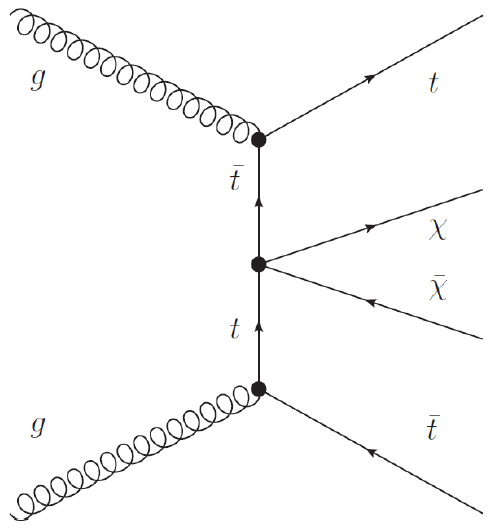
\includegraphics[width=0.30\textwidth]{figures/eft.png}}
  \hspace{2cm}
  \subfigure[]{\label{subfig:sms}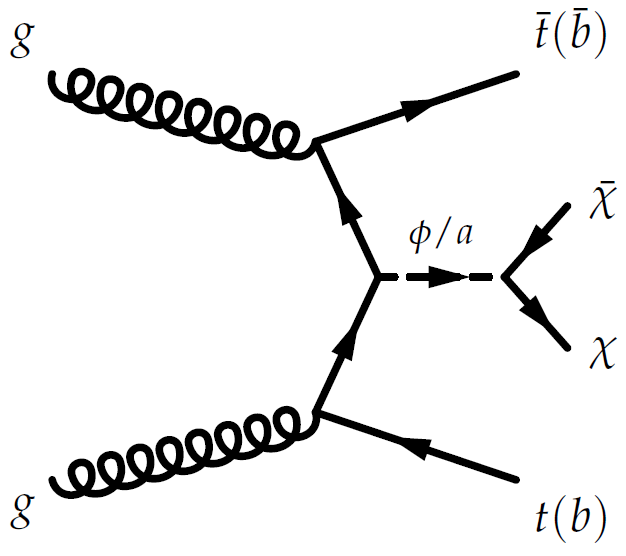
\includegraphics[width=0.35\textwidth]{figures/sms.png}}
  \caption{Diagrams for \subref{subfig:eft} effective field theory and \subref{subfig:sms} and simplified model.}
  \label{fig:ttdm_diagrams}
\end{center}
\end{figure}

\begin{table}[!ht]
\centering
\begin{tabular}{|l|ccccccccc|}
\hline
  \multicolumn{1}{|c|}{$M_{\chi}$ ($\GeV$)} & \multicolumn{9}{|c|}{$M_{\mbox{\scriptsize{med}}}$ ($\GeV$)} \\
\hline
  $1$    & $10$ & $20$ & $50$ & $100$ & $200$ & $300$ & $500$ & $1000$ & $10000$ \\
  $10$   & $10$ & $15$ & $50$ & $100$ &       &       &       &        & $10000$ \\
  $50$   & $10$ &      & $50$ & $95$  & $200$ & $300$ &       &        & $10000$ \\
  $150$  & $10$ &      &      &       & $200$ & $295$ & $500$ & $1000$ & $10000$ \\
  $500$  & $10$ &      &      &       &       &       & $500$ & $995$  & $10000$ \\
  $1000$ & $10$ &      &      &       &       &       &       & $1000$ & $10000$ \\
\hline
\end{tabular}
\caption{Simplified model benchmarks for $s$-channel simplified models with spin-$0$ mediators decaying to Dirac DM fermions.}
\label{tab:dmf}
\end{table}

\subsection{Analysis Strategy Overview}
\label{subsec:intro_anastrat}
This analysis approach is a categorized \met-shape fit, where the categories are formed based on resolved top tagging variables. As a reference, we also pursue a simple Poisson counting analysis with both categorized and uncategorized cases.


%\clearpage
 
\section{Samples}
\label{sec:datasets}

This analysis is based on the data sample recorded by CMS at the center-of-mass energy $\sqrt{s}=13\:\TeV\:$ during 2015 LHC operation. The dataset corresponds to an integrated luminosity of $1.27\:\ifb\:$. The dataset names are listed in Table~\ref{tab:data}.

\begin{table}[!ht]
\centering
\begin{tabular}{|l|l|}
\hline
Dataset \\
\hline
METRun2015D-PromptReco-v3 \\
METRun2015D-PromptReco-v4 \\
\hline
SingleMu2015D-PromptReco-v3 \\
SingleMu2015D-PromptReco-v4  \\
\hline
SingleEle2015D-PromptReco-v3 \\
SingleEle2015D-PromptReco-v4 \\
\hline
Photon2015D-PromptReco-v3   \\
Photon2015D-PromptReco-v4   \\
\hline
\end{tabular}
\caption{Datasets used in the presented analysis}
\label{tab:data}
\end{table}

Monte Carlo (MC) simulation samples used in this study come from the ``Spring15'' production campaign. The simulated beam conditions correspond to $25\,\mbox{ns}$ bunch crossings and 20 pileup interactions on average. For signal samples, both EFT signals and simplified models have been produced. The EFT models were generated with $M_*=1000\:\GeV$ and the various $M_\chi$ points that were produced are listed in Table~\ref{tab:ttdm_samples}. The simplified models were generated for various points ranging in $10\:\GeV\:<M_{\phi}<1\:\TeV\:$ for scalar and pseudo-scalar mediators and DM particles ranging in $1\:\GeV\:< M_{\chi}<150\:\GeV\:$ and are listed in Table~\ref{tab:ttdm_simplified}. Note that for the EFT model cross sections used to normalize the signal samples correspond to $M_*=100\:\GeV$, as this is closer to the limits from Run-1 results and allows better visualization of the signal when plotting.

\begin{table}[!ht]
\centering
\begin{tabular}{|l|l|}
\hline
  Sample name                                          & $\sigma$ [$\pb$] \\
\hline
  /TTDMDMJets\_M1GeV\_Tune4C\_13TeV-madgraph-tauola    & $1.320$ \\
  /TTDMDMJets\_M10GeV\_Tune4C\_13TeV-madgraph-tauola   & $1.322$ \\
  /TTDMDMJets\_M50GeV\_Tune4C\_13TeV-madgraph-tauola   & $1.187$ \\
  /TTDMDMJets\_M100GeV\_Tune4C\_13TeV-madgraph-tauola  & $0.9553$ \\
  /TTDMDMJets\_M200GeV\_Tune4C\_13TeV-madgraph-tauola  & $0.6301$ \\
  /TTDMDMJets\_M600GeV\_Tune4C\_13TeV-madgraph-tauola  & $0.1038$ \\
  /TTDMDMJets\_M1000GeV\_Tune4C\_13TeV-madgraph-tauola & $0.01585$ \\
\hline
\end{tabular}
\caption{EFT signal samples and cross sections. The cross sections correspond to $M_{*}=100\:\GeV$.}
\label{tab:ttdm_samples}
\end{table}


\begin{table}[!ht]
\centering
\begin{tabular}{|l|l|}
\hline
Sample name                                    & $\sigma$ [$\pb$]\\
\hline
/TTbarDMJets\_pseudoscalar\_Mchi-10\_Mphi-100\_TuneCUETP8M1\_13TeV-madgraphMLM-pythia8          & $0.1863543$ \\
/TTbarDMJets\_pseudoscalar\_Mchi-10\_Mphi-10\_TuneCUETP8M1\_13TeV-madgraphMLM-pythia8            & $0.0147397$ \\
/TTbarDMJets\_pseudoscalar\_Mchi-150\_Mphi-1000\_TuneCUETP8M1\_13TeV-madgraphMLM-pythia8      & $0.0003392$ \\
/TTbarDMJets\_pseudoscalar\_Mchi-150\_Mphi-200\_TuneCUETP8M1\_13TeV-madgraphMLM-pythia8      &  $0.0003856$ \\
/TTbarDMJets\_pseudoscalar\_Mchi-150\_Mphi-500\_TuneCUETP8M1\_13TeV-madgraphMLM-pythia8      & $0.0048655$ \\
/TTbarDMJets\_pseudoscalar\_Mchi-1\_Mphi-100\_TuneCUETP8M1\_13TeV-madgraphMLM-pythia8      & $0.1820882$ \\
/TTbarDMJets\_pseudoscalar\_Mchi-1\_Mphi-10\_TuneCUETP8M1\_13TeV-madgraphMLM-pythia8      &   $0.4689972$ \\
/TTbarDMJets\_pseudoscalar\_Mchi-1\_Mphi-200\_TuneCUETP8M1\_13TeV-madgraphMLM-pythia8      &  $0.0877421$ \\ 
/TTbarDMJets\_pseudoscalar\_Mchi-1\_Mphi-20\_TuneCUETP8M1\_13TeV-madgraphMLM-pythia8      &    $0.4134034$ \\
/TTbarDMJets\_pseudoscalar\_Mchi-1\_Mphi-300\_TuneCUETP8M1\_13TeV-madgraphMLM-pythia8      &  $0.0389858$ \\
/TTbarDMJets\_pseudoscalar\_Mchi-1\_Mphi-500\_TuneCUETP8M1\_13TeV-madgraphMLM-pythia8      &  $0.0047980$ \\
/TTbarDMJets\_pseudoscalar\_Mchi-1\_Mphi-50\_TuneCUETP8M1\_13TeV-madgraphMLM-pythia8      &  $0.3353931$ \\
/TTbarDMJets\_pseudoscalar\_Mchi-50\_Mphi-200\_TuneCUETP8M1\_13TeV-madgraphMLM-pythia8      &$0.0881722$ \\
/TTbarDMJets\_pseudoscalar\_Mchi-50\_Mphi-300\_TuneCUETP8M1\_13TeV-madgraphMLM-pythia8      &$0.0431273$ \\
/TTbarDMJets\_pseudoscalar\_Mchi-50\_Mphi-50\_TuneCUETP8M1\_13TeV-madgraphMLM-pythia8      &$0.0027793$ \\
\hline
/TTbarDMJets\_scalar\_Mchi-10\_Mphi-100\_TuneCUETP8M1\_13TeV-madgraphMLM-pythia8      &  $0.7014639$ \\
/TTbarDMJets\_scalar\_Mchi-150\_Mphi-200\_TuneCUETP8M1\_13TeV-madgraphMLM-pythia8      &$0.0001263$ \\
/TTbarDMJets\_scalar\_Mchi-1\_Mphi-1000\_TuneCUETP8M1\_13TeV-madgraphMLM-pythia8      &  $0.0003497$ \\
/TTbarDMJets\_scalar\_Mchi-1\_Mphi-10\_TuneCUETP8M1\_13TeV-madgraphMLM-pythia8      & $17.896528$ \\
/TTbarDMJets\_scalar\_Mchi-1\_Mphi-20\_TuneCUETP8M1\_13TeV-madgraphMLM-pythia8      & $10.532532$ \\
/TTbarDMJets\_scalar\_Mchi-1\_Mphi-500\_TuneCUETP8M1\_13TeV-madgraphMLM-pythia8      &$0.0048826$ \\
/TTbarDMJets\_scalar\_Mchi-1\_Mphi-50\_TuneCUETP8M1\_13TeV-madgraphMLM-pythia8      &$3.0348248$ \\
/TTbarDMJets\_scalar\_Mchi-50\_Mphi-300\_TuneCUETP8M1\_13TeV-madgraphMLM-pythia8      &$0.0312498$ \\
/TTbarDMJets\_scalar\_Mchi-50\_Mphi-50\_TuneCUETP8M1\_13TeV-madgraphMLM-pythia8      &$0.0027578$ \\
/TTbarDMJets\_scalar\_Mchi-1\_Mphi-100\_TuneCUETP8M1\_13TeV-madgraphMLM-pythia8      &$0.6906371$ \\
/TTbarDMJets\_scalar\_Mchi-50\_Mphi-200\_TuneCUETP8M1\_13TeV-madgraphMLM-pythia8      &$0.1109005$\\
\hline
\end{tabular}
\caption{Simplified model signal samples for scalar and pseudo-scalar $M_{\phi}$ and cross sections.}
\label{tab:ttdm_simplified}
\end{table}

The MC samples for SM processes and their respective cross section are listed in Table~\ref{tab:mc_samples}. %Note that diboson (\WW, \WZ, \ZZ) samples were not produced in Phys14.

\begin{sidewaystable}
%\begin{table}[!ht]
\centering
\begin{tabular}{|l|l|r|}
\hline
  Process & Sample name & $\sigma$ [$\pb$] \\
\hline
  \ttbar & Spring15\_a25ns\_TTJets\_madgraph\_MINIAOD & $831.76$ \\
           & Spring15\_a25ns\_TTJets\_amcatnlo\_MINIAOD   & $831.76$ \\
\hline
  \W\To\Lep\Nu & Spring15\_a25ns\_WJetsToLNu\_MINIAOD & $61526.7$ \\
  			& Spring15\_a25ns\_WJetsToLNu\_HT-100to200\_TuneCUETP8M1\_13TeV-madgraphMLM-pythia8\_MINIAOD & $1627.450$\\
			& Spring15\_a25ns\_WJetsToLNu\_HT-200to400\_TuneCUETP8M1\_13TeV-madgraphMLM-pythia8\_MINIAOD & $435.237$\\
			& Spring15\_a25ns\_WJetsToLNu\_HT-400to600\_TuneCUETP8M1\_13TeV-madgraphMLM-pythia8\_MINIAOD & $ 59.181$\\
			& Spring15\_a25ns\_WJetsToLNu\_HT-600to800\_TuneCUETP8M1\_13TeV-madgraphMLM-pythia8\_MINIAOD & $14.581$\\
			& Spring15\_a25ns\_WJetsToLNu\_HT-800to1200\_TuneCUETP8M1\_13TeV-madgraphMLM-pythia8\_MINIAOD & $6.656$\\
			& Spring15\_a25ns\_WJetsToLNu\_HT-1200to2500\_TuneCUETP8M1\_13TeV-madgraphMLM-pythia8\_MINIAOD & $1.608$ \\
			& Spring15\_a25ns\_WJetsToLNu\_HT-2500toInf\_TuneCUETP8M1\_13TeV-madgraphMLM-pythia8\_MINIAOD & $0.0389$ \\
%               & /WJetsToLNu\_HT-200to400\_Tune4C\_13TeV-madgraph-tauola & $580.068$ \\
  %             & /WJetsToLNu\_HT-400to600\_Tune4C\_13TeV-madgraph-tauola & $68.4$ \\
    %           & /WJetsToLNu\_HT-600toInf\_Tune4C\_13TeV-madgraph-tauola & $23.136$ \\
\hline
  \Z\To\Lep\Lep  & Spring15\_a25ns\_DYJetsToLL\_M-50\_TuneCUETP8M1\_13TeV-amcatnloFXFX-pythia8\_MINIAOD                & $6025.2$ \\
  			

  
  %& /DYJetsToLL\_M-50\_HT-100to200\_Tune4C\_13TeV-madgraph-tauola & $213.536$ \\
                %& /DYJetsToLL\_M-50\_HT-200to400\_Tune4C\_13TeV-madgraph-tauola & $57.412$ \\
                %& /DYJetsToLL\_M-50\_HT-400to600\_Tune4C\_13TeV-madgraph-tauola & $7.194$ \\
                %& /DYJetsToLL\_M-50\_HT-600toInf\_Tune4C\_13TeV-madgraph-tauola & $2.395$ \\
\hline
  \Z\To\Nu\Nu & Spring15\_a25ns\_ZJetsToNuNu\_HT-100To200\_13TeV-madgraph\_MINIAOD & $344.978$\\
			& Spring15\_a25ns\_ZJetsToNuNu\_HT-200To400\_13TeV-madgraph\_MINIAOD & $96.383$\\
			& Spring15\_a25ns\_ZJetsToNuNu\_HT-400To600\_13TeV-madgraph\_MINIAOD & $13.456$\\
			& Spring15\_a25ns\_ZJetsToNuNu\_HT-600ToInf\_13TeV-madgraph\_MINIAOD & $5.166$\\
  		     
  %& /ZJetsToNuNu\_HT-100to200\_Tune4C\_13TeV-madgraph-tauola & $409.487$ \\
     %         & /ZJetsToNuNu\_HT-200to400\_Tune4C\_13TeV-madgraph-tauola & $110.779$ \\
        %      & /ZJetsToNuNu\_HT-400to600\_Tune4C\_13TeV-madgraph-tauola & $13.177$ \\
           %   & /ZJetsToNuNu\_HT-600toInf\_Tune4C\_13TeV-madgraph-tauola & $4.52$ \\
\hline
  Single \Top & Spring15\_a25ns\_ST\_t-channel\_top\_4f\_leptonDecays\_13TeV-powheg-pythia8\_TuneCUETP8M1\_MINIAOD     & $ 136.02 $ \\
  			& Spring15\_a25ns\_ST\_t-channel\_antitop\_4f\_leptonDecays\_13TeV-powheg-pythia8\_TuneCUETP8M1\_MINIAOD   & $80.95  $ \\
			& Spring15\_a25ns\_ST\_tW\_top\_5f\_inclusiveDecays\_13TeV-powheg-pythia8\_TuneCUETP8M1\_MINIAOD	           & $35.6$ \\   
  			& Spring15\_a25ns\_ST\_tW\_antitop\_5f\_inclusiveDecays\_13TeV-powheg-pythia8\_TuneCUETP8M1\_MINIAOD             & $ 35.6$\\

  			
  % /TToLeptons\_t-channel-CSA14\_Tune4C\_13TeV-aMCatNLO-tauola     & $44.0802$ \\
            % & /TBarToLeptons\_t-channel\_Tune4C\_CSA14\_13TeV-aMCatNLO-tauola & $26.2343$ \\
             % & /TToLeptons\_s-channel-CSA14\_Tune4C\_13TeV-aMCatNLO-tauola     & $2.3328$ \\
             % & /TBarToLeptons\_s-channel-CSA14\_Tune4C\_13TeV-aMCatNLO-tauola  & $1.3478$ \\
             % & /T\_tW-channel-DR\_Tune4C\_13TeV-CSA14-powheg-tauola            & $35.6$ \\
             % & /Tbar\_tW-channel-DR\_Tune4C\_13TeV-CSA14-powheg-tauola         & $35.6$ \\ 
%\hline
 % \ttbar\W & & $ $\\%& /TTWJets\_Tune4C\_13TeV-madgraph-tauola & $0.72$ \\
 % \ttbar\Z  & & $ $\\%& /TTZJets\_Tune4C\_13TeV-madgraph-tauola & $0.70$ \\
\hline
  Diboson   & Spring15\_a25ns\_WWTo2L2Nu\_13TeV-powheg\_MINIAOD & $12.178$ \\	
  		 & Spring15\_a25ns\_WWToLNuQQ\_13TeV-powheg\_MINIAOD & $49.997$ \\
		 & Spring15\_a25ns\_WWTo4Q\_13TeV-powheg\_MINIAOD & $51.723$ \\	
  		 & Spring15\_a25ns\_WZ\_TuneCUETP8M1\_13TeV-pythia8\_MINIAOD & $ 48.4 $ \\ 
  		 & Spring15\_a25ns\_ZZ\_TuneCUETP8M1\_13TeV-pythia8\_MINIAOD & $ 19.3 $ \\
\hline
QCD &   Spring15\_a25ns\_QCD\_HT100to200\_TuneCUETP8M1\_13TeV-madgraphMLM-pythia8\_MINIAOD & $2.785\times10^{7}$\\
         &   Spring15\_a25ns\_QCD\_HT200to300\_TuneCUETP8M1\_13TeV-madgraphMLM-pythia8\_MINIAOD & $1.717\times10^{6}$\\
         &   Spring15\_a25ns\_QCD\_HT300to500\_TuneCUETP8M1\_13TeV-madgraphMLM-pythia8\_MINIAOD & $3.513\times10^{5}$\\
         &   Spring15\_a25ns\_QCD\_HT500to700\_TuneCUETP8M1\_13TeV-madgraphMLM-pythia8\_MINIAOD & $3.163\times10^{4}$\\
         &   Spring15\_a25ns\_QCD\_HT700to1000\_TuneCUETP8M1\_13TeV-madgraphMLM-pythia8\_MINIAOD & $6.802\times10^{3}$ \\
         &   Spring15\_a25ns\_QCD\_HT1000to1500\_TuneCUETP8M1\_13TeV-madgraphMLM-pythia8\_MINIAOD & $1.206\times10^{3}$\\
         &   Spring15\_a25ns\_QCD\_HT1500to2000\_TuneCUETP8M1\_13TeV-madgraphMLM-pythia8\_MINIAOD & $120.4$\\
         &   Spring15\_a25ns\_QCD\_HT2000toInf\_TuneCUETP8M1\_13TeV-madgraphMLM-pythia8\_MINIAOD     & $25.24$\\
  %QCD & /QCD\_HT\_250To500\_13TeV-madgraph (v1 \& ext1-v2)  & $670500$ \\
     % & /QCD\_HT-500To1000\_13TeV-madgraph (v1 \& ext1-v1)  & $26740$ \\
     % & /QCD\_HT\_1000ToInf\_13TeV-madgraph (v1 \& ext1-v1) & $769.7$ \\
\hline
\end{tabular}
\caption{MC samples and cross sections for SM processes.}
\label{tab:mc_samples}
\end{sidewaystable}
%\end{table}


\clearpage

\section{Physics Objects}
\label{sec:objects}

\subsection{Electrons}
\label{subsec:obj_electron}

Electrons are selected using cut-based strategies. ``Tight'' and ``Veto'' working points (WP) from the ``V1'' set of prescriptions tuned on Spring15 25 ns samples are applied in the analysis. ``Tight'' electrons are used to select events with semileptonic top-pairs, while ``Veto'' electrons are used for rejecting events with extra electrons. The variables and cuts defining the working points are listed in Table~\ref{tab:ele_wp}. The isolation quantity is based on PF-candidates within $R=0.3$ from the electron and pileup effects are mitigated using the effective area corrections listed in Table~\ref{tab:ea}. %$\Delta\beta$ method, which subtracts neutral contributions due to pileup -- this contribution is estimated as half the $\pt$ sum of charged particles not originating from the primary vertex. The isolation is computed as,
%\begin{equation}
%  I = I_{h^+} + \max\left(I_{h^0} + I_{\gamma} - 0.5*I_{\mbox{\scriptsize{pileup}}} , 0\right),
%\end{equation}
%where $I_{h^+}$, $I_{h^0}$, $I_{\gamma}$, and $I_{\mbox{\scriptsize{pileup}}}$ are the contributions from charged hadrons, neutral hadrons, photons, and charged hadrons from pileup, respectively.


\begin{table}[!ht]
\centering
\begin{tabular}{|c|c|c|c|c|}
\hline
  & \multicolumn{2}{|c|}{Veto WP} & \multicolumn{2}{|c|}{Tight WP} \\
  Variable                                                  & Barrel     & Endcap     & Barrel     & Endcap     \\
\hline
  $\sigma_{i\eta i\eta} <$               		& $0.0114$ & $0.0352$ & $0.0101$ & $0.0279$ \\
  $\Delta\eta_{\mbox{\scriptsize{in}}} <$ 	& $0.0152$ & $0.0113$ & $0.00926$   & $0.00724$ \\
  $\Delta\phi_{\mbox{\scriptsize{in}}} <$ 	& $0.216$   & $0.237$ &   $0.0336  $ & $0.0918$ \\
  $H/E$                                   			& $0.181$   & $0.116$ &   $0.0597  $ & $0.0615$ \\
  $|1/E - 1/p| <$                         			& $0.207$   & $0.174$ &   $0.012$ & $0.00999$ \\
  $|d_0|$ (cm) $<$                     			& $0.0564$ & $0.222$ &   $0.0111$ & $0.0351$ \\
  $|d_z|$ (cm) $<$                     			& $0.472$   & $0.921$ &   $0.0466$ & $0.417$ \\
  No. of missing expected hits $\leq$      & $2$           & $3$        &   $2$              & $1$        \\
  relative isolation $<$                             & $0.126$ & $0.144$ & $0.0354$ & $0.0646$ \\
  pass conversion veto                             & true       & true       & true       & true       \\
\hline
\end{tabular}
\caption{Variables and thresholds that define ``Veto'' and ``Tight'' electrons in the Spring15 25 ns ``V1'' cut-based selections \cite{electron} as per the official Run 2 recommendations. An electron is in the barrel if it has supercluster $|\eta|<1.479$, otherwise it is in the endcap.}
\label{tab:ele_wp}
\end{table}

\begin{table}[!ht]
\centering
\begin{tabular}{|c|c|}
\hline
$|\eta|$ range          &  $A_{eff}$ for $h_{0} + \gamma$ \\
\hline
$ 0.0 - 1.0$              &  0.1752 \\
\hline
$ 1.0 - 1.479$           &  0.8762 \\
\hline
$1.479 - 2.0$            &  0.1411 \\
\hline
$2.0 - 2.2$                & 0.1534 \\
\hline
$2.2 - 2.3$                & 0.1903 \\
\hline
$2.3 - 2.4$                & 0.2243 \\
\hline
\end{tabular}
\caption{Effective areas for electron ID PU correction as recommended \cite{EA}}
\label{tab:ea}
\end{table}

Electron selection efficiencies are measured with the tag-and-probe method. The efficiencies measured in data and the Drell-Yan MC sample are shown in Fig.~\ref{fig:elvetoeff} and Fig.~\ref{fig:eltighteff}. Data-to-MC tight electron selection efficiency scale factors are shown in Table ~\ref{tab:eletight_sf} and Fig.~\ref{fig:ele_sf}. Scale factors for the veto electron ID are shown in Table~\ref{tab:eleveto_sf} and Fig.~\ref{fig:ele_sf}. The ratio of efficiencies measured in data and MC is used to perform corrections to MC-derived yields for the search analysis.


\begin{table}[!ht]
\centering
\begin{tabular}{|c|c|c|c|c|}
\hline
&                          &                              &                                         &       \\
  & $0.0 < |\eta| < 1.4$ & $1.4 < |\eta| < 1.6$ & $1.6 < |\eta| < 2.1$ & $2.1 < |\eta| < 2.5$ \\
  &                          &                              &                                         & \\
\hline	
$30 < \pt <  40$ &  $0.981 \pm  0.002$  & $ 0.929 \pm  0.010$  &  $0.971 \pm  0.008$  &  $0.998 \pm  0.007$ \\
\hline
$40 < \pt <  50$ & $ 0.975 \pm  0.002 $ &  $0.968 \pm  0.007$  &  $0.987 \pm  0.005$  &  $1.008 \pm  0.006$ \\
\hline 
$50 < \pt < 100$ &  $0.976 \pm  0.003 $ &  $0.996 \pm  0.013$  &  $0.981 \pm  0.013$  &  $1.010 \pm  0.015$ \\
\hline
$100 < \pt < 150$ &  $0.977 \pm  0.011$  &  $0.983 \pm  0.044$  &  $0.996 \pm  0.025$  &  $0.985 \pm  0.050$ \\
\hline    
      $\pt > 150$ &  $1.008 \pm  0.021$  &  $1.045 \pm  0.080$  &  $0.977 \pm  0.047$  &  $0.823 \pm  0.073$ \\
\hline
\end{tabular}	
\caption{Tight electron selection efficiency scale factors for electrons with $\pt>30\:\GeV\:$}
\label{tab:eletight_sf}
\end{table}

\begin{table}[!ht]
\centering
\begin{tabular}{|c|c|c|c|c|}
\hline
&                             &                            &                             &                           \\
 & $0.0 < |\eta| < 1.4$ & $1.4 < |\eta| < 1.6$ & $1.6 < |\eta| < 2.1$ & $2.1 < |\eta| < 2.5$ \\
&                             &                            &                             &                           \\
\hline
 $10 < \pt <  15$ &  $0.992 \pm  0.015$  & $ 0.882 \pm  0.102$  &  $1.059 \pm  0.055  $&  $1.071 \pm  0.039 $\\
\hline
 $15 < \pt <  20$ &  $0.990 \pm  0.003 $ &  $0.739 \pm  0.052 $ &  $0.972 \pm  0.072  $&  $1.024 \pm  0.020 $\\
\hline
 $20 < \pt <  25$ &  $0.989 \pm  0.003 $ &  $0.907 \pm  0.038 $ &  $0.995 \pm  0.011  $&  $1.014 \pm  0.012 $\\
 \hline
 $25 < \pt <  30$ &  $0.982 \pm  0.004 $ &  $0.940 \pm  0.044 $ &  $1.005 \pm  0.002  $&  $1.018 \pm  0.009 $ \\
 \hline
 $30 < \pt <  40$ &  $0.993 \pm  0.001 $ &  $0.959 \pm  0.005 $ &  $1.014 \pm  0.005  $&  $1.010 \pm  0.004 $\\
 \hline
 $40 < \pt <  50$ &  $0.992 \pm  0.001 $ &  $0.986 \pm  0.002 $ &  $1.016 \pm  0.002  $&  $1.012 \pm  0.003 $\\
 \hline
 $50 < \pt < 100$ & $ 0.993 \pm  0.004 $ & $ 0.990 \pm  0.009 $ & $ 1.006 \pm  0.012 $ & $ 1.017 \pm  0.007$ \\
\hline
$100 < \pt < 150$ & $ 0.996 \pm  0.007 $ & $ 1.010 \pm  0.031 $ & $ 1.013 \pm  0.016 $ & $ 0.998 \pm  0.020 $\\
 \hline 
  $    \pt > 150$ & $ 0.988 \pm  0.007 $ &  $0.988 \pm  0.044 $ & $ 1.006 \pm  0.036 $ & $ 0.990 \pm  0.990 $\\
\hline
\end{tabular}	
\caption{Veto electron ID efficiency scale factors for electrons with $\pt>10\:\GeV\:$}
\label{tab:eleveto_sf}
\end{table}

\begin{figure}[htbp]
\begin{center}
  \subfigure[]{\label{sub fig:eletightsf}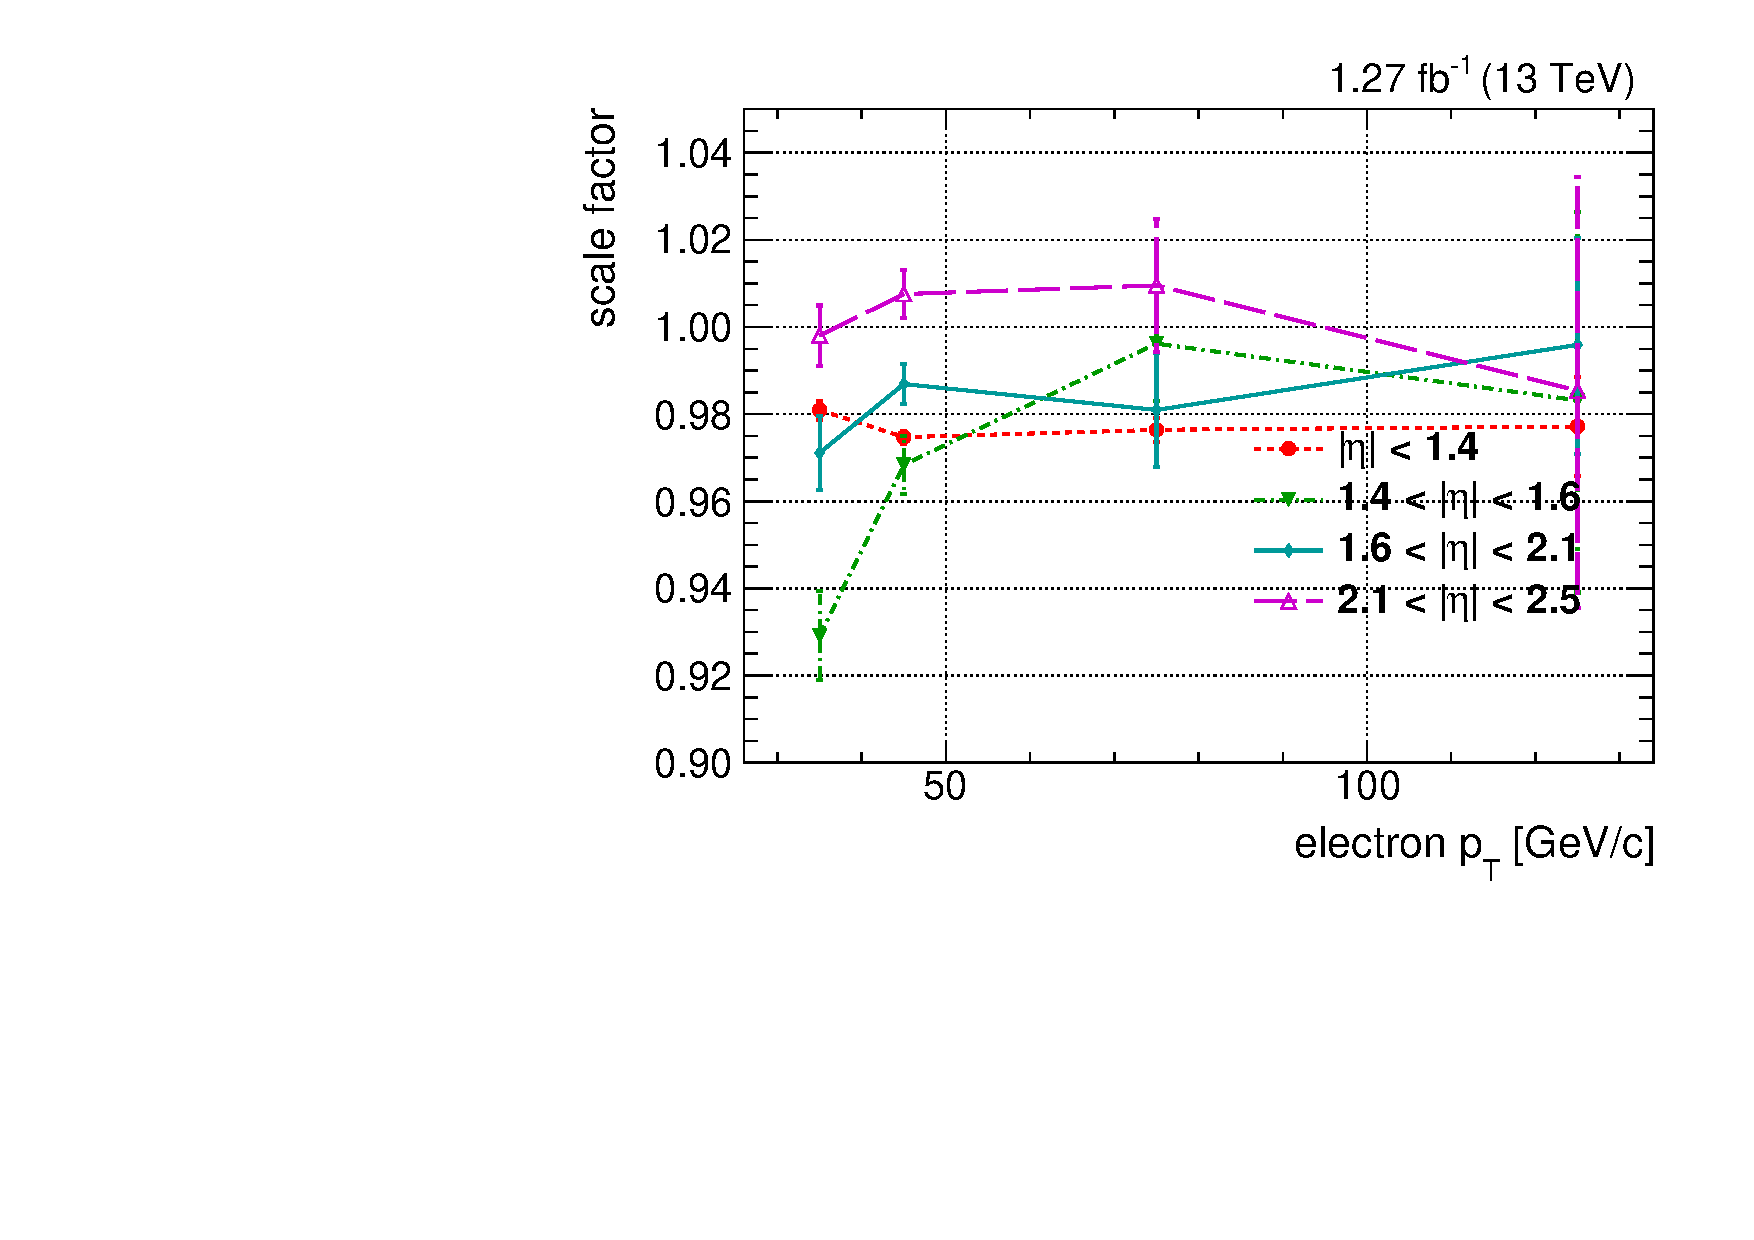
\includegraphics[width=0.48\textwidth]{figures/eletight_sfetapt.pdf}}
  \subfigure[]{\label{sub fig:eleloosesf}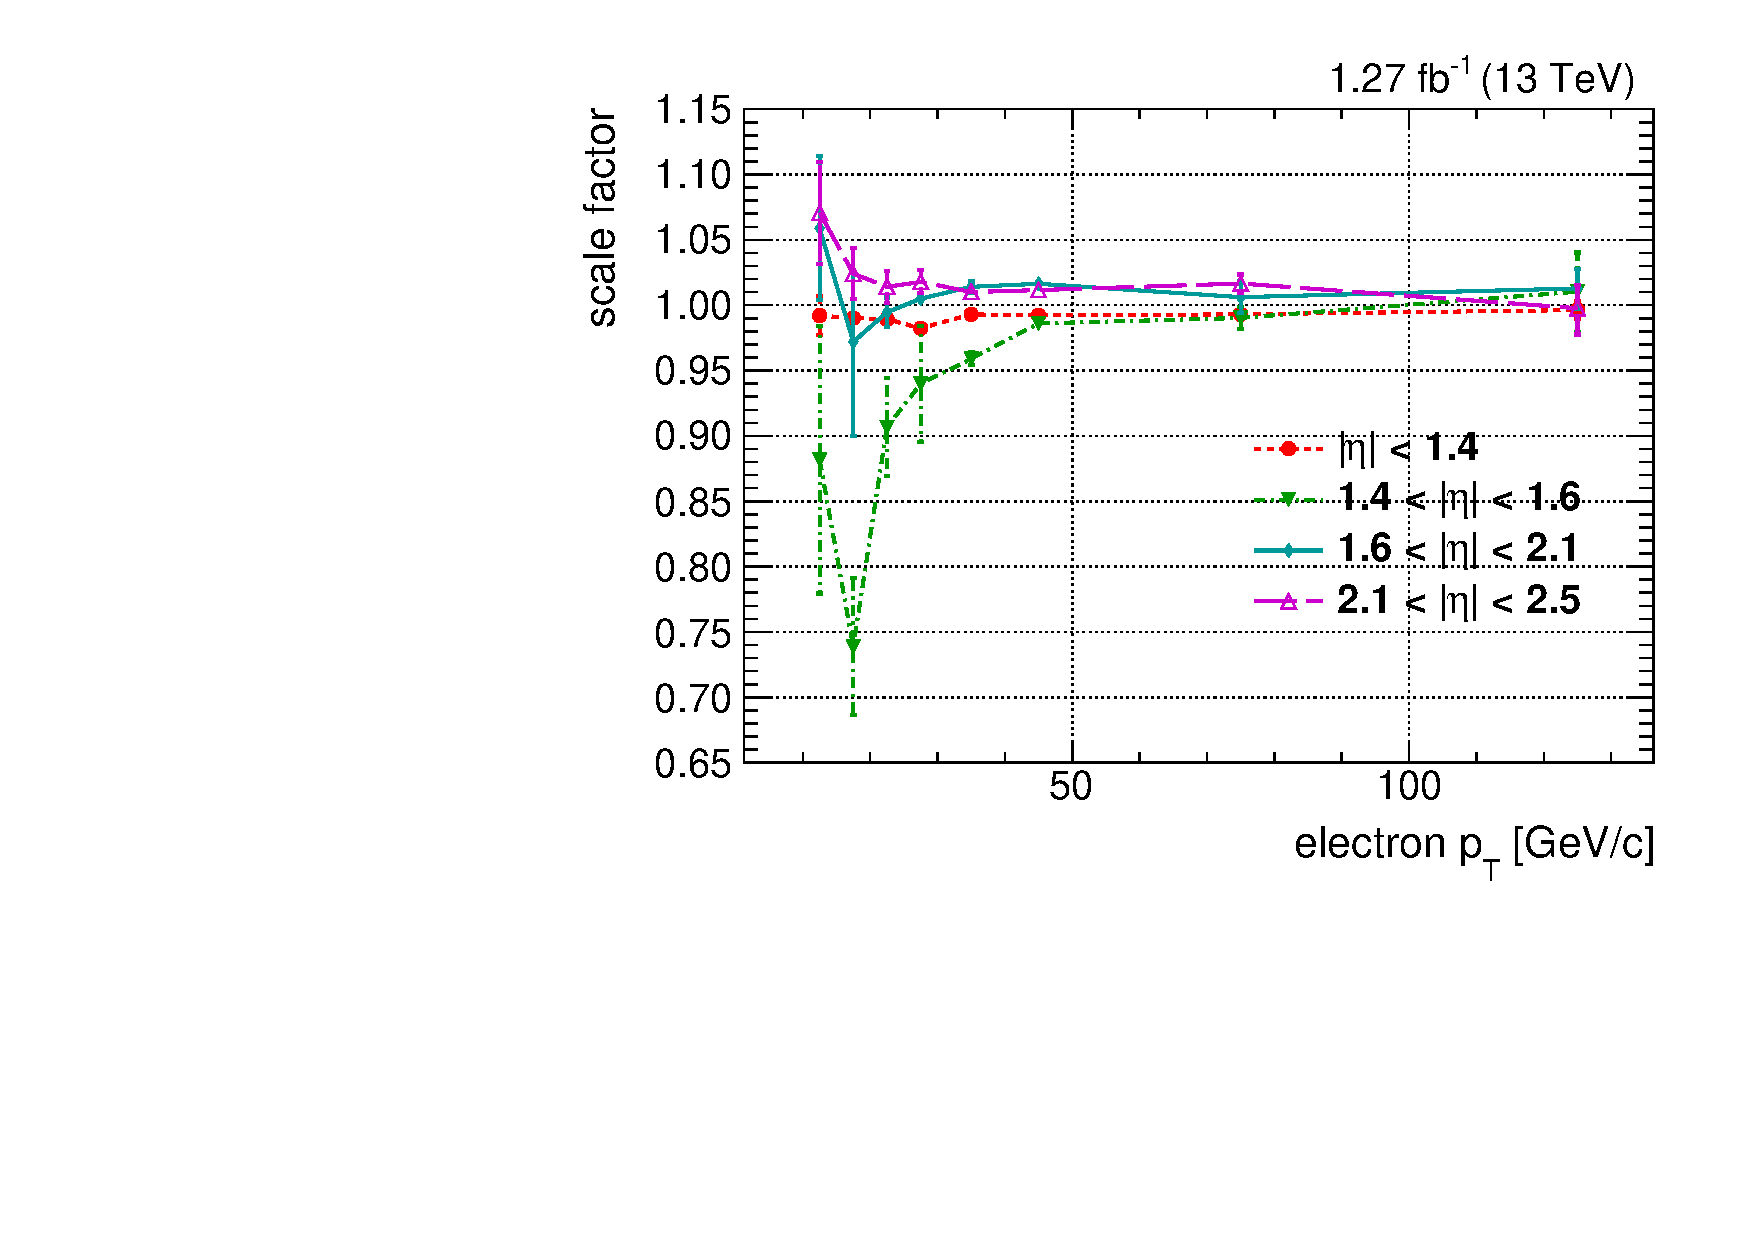
\includegraphics[width=0.48\textwidth]{figures/elveto_sfetapt.pdf}}
  \caption{Electron ``Tight" WP (left) and ``Veto" WP (right) data-to-MC efficiency scale factors as a function of electron $\pt$ for various $|\eta|$ bins.}
  \label{fig:ele_sf}	
\end{center}
\end{figure}

\begin{figure}[htbp]
\begin{center}
  \subfigure[]{\label{subfig:elvetoeffeta}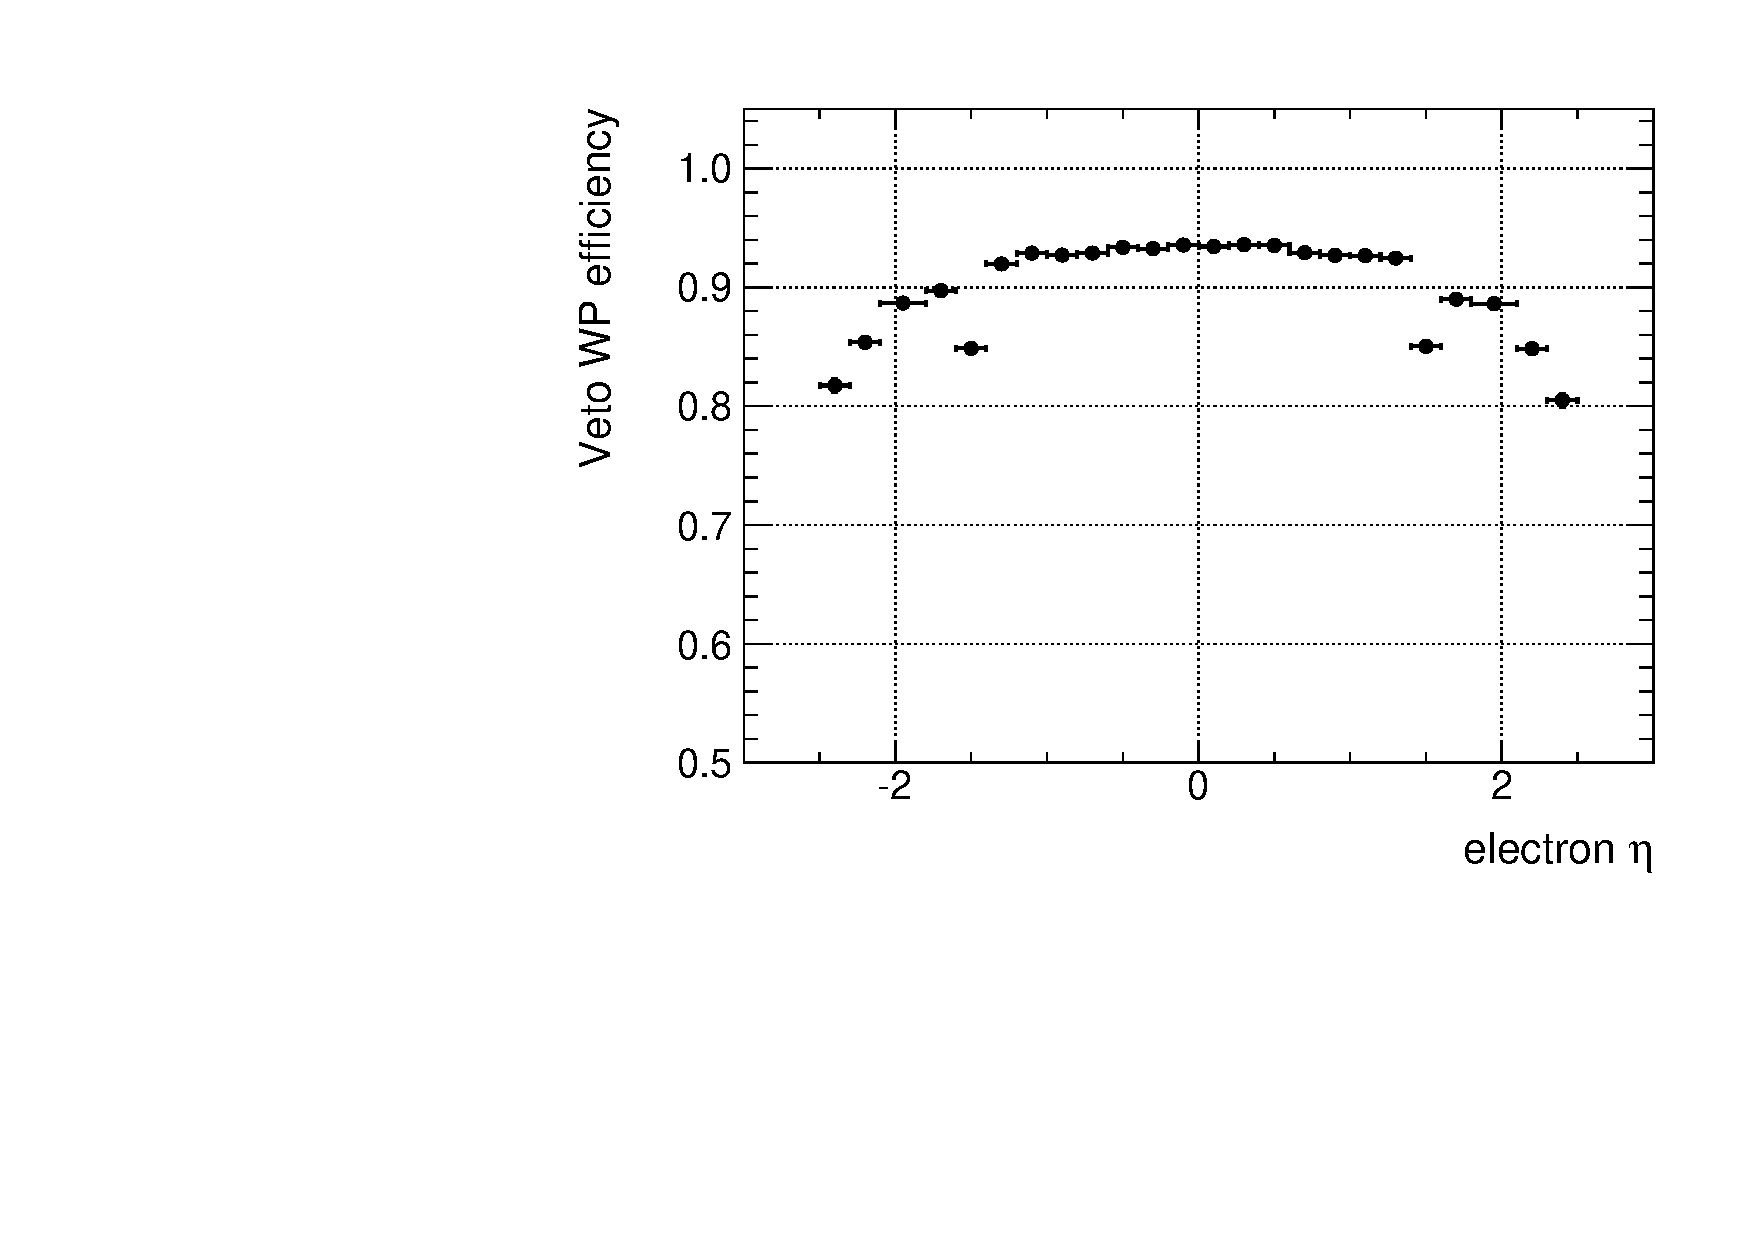
\includegraphics[width=0.48\textwidth]{figures/elveto_effeta.pdf}}
  \subfigure[]{\label{subfig:elvetoeffpt}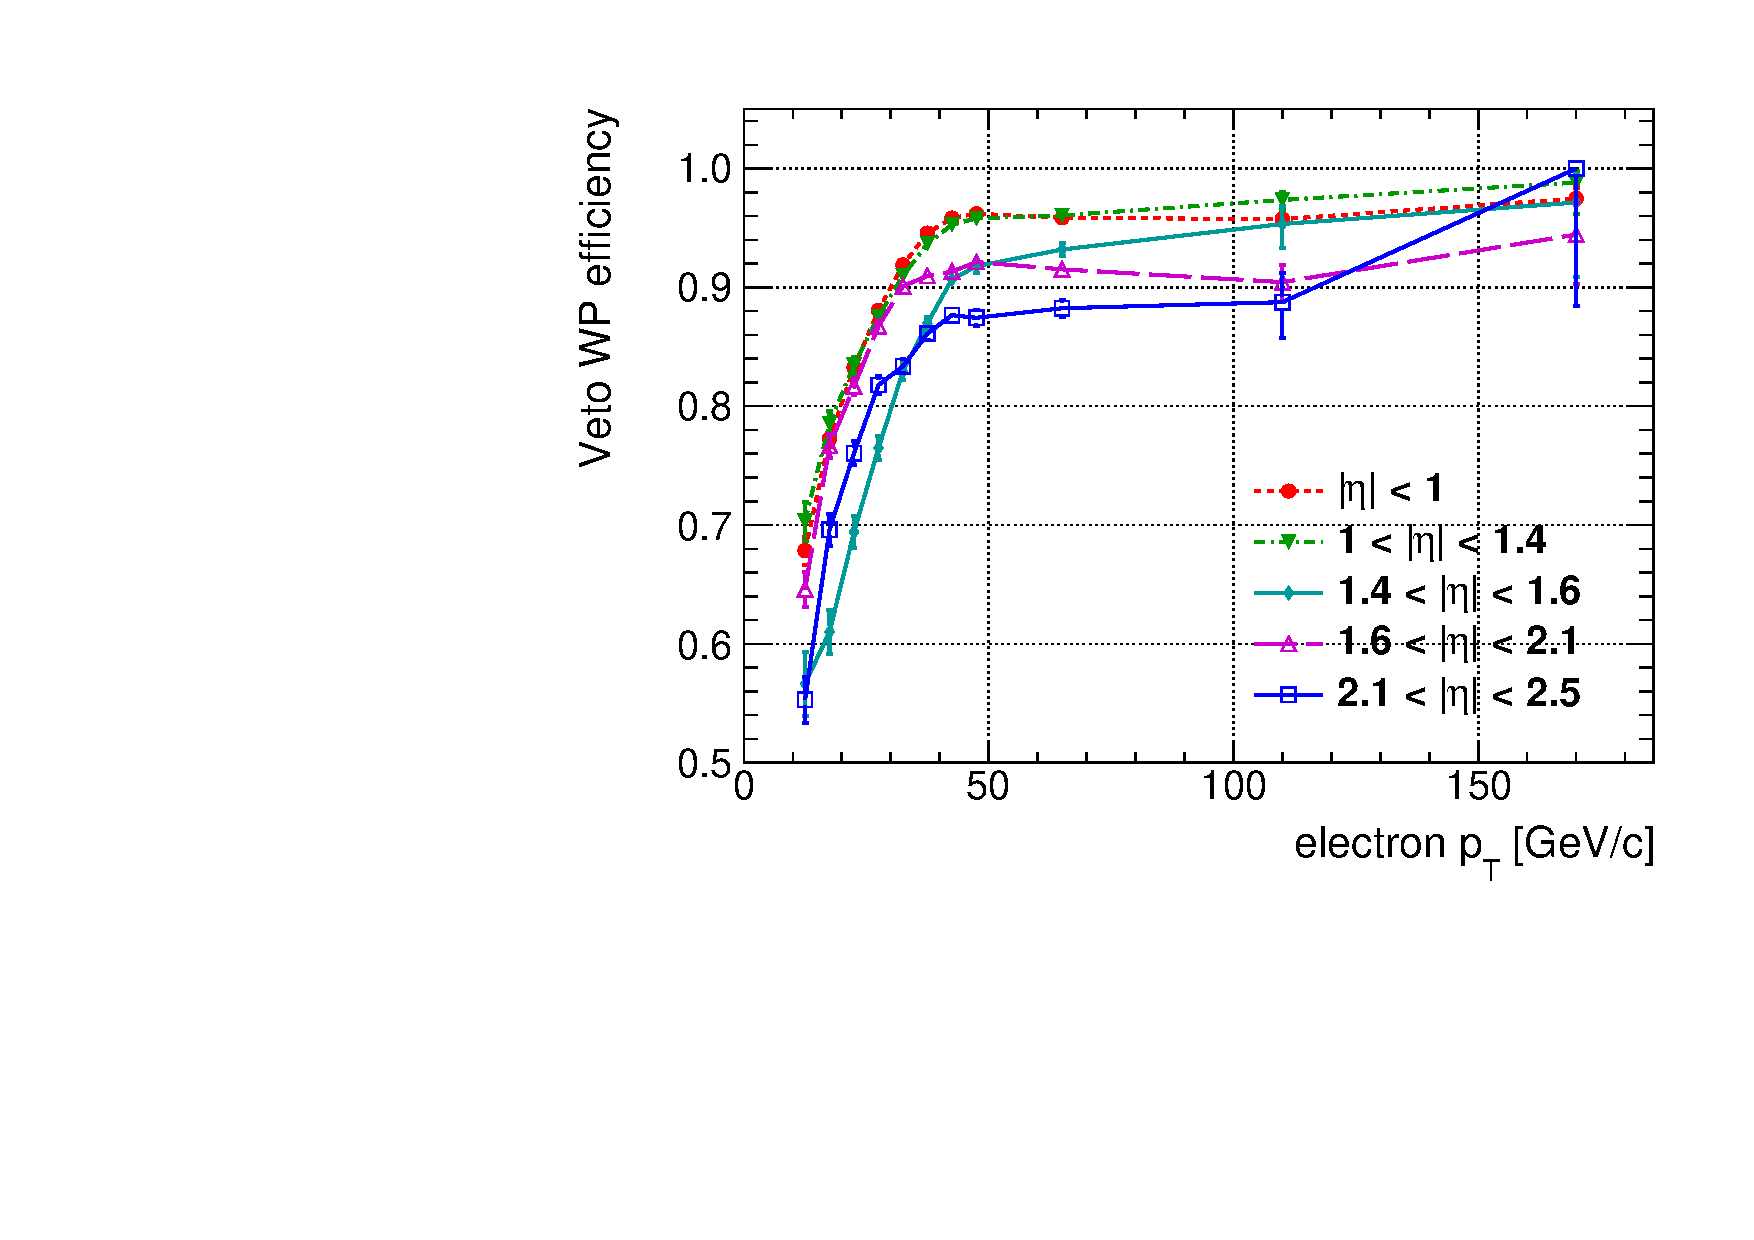
\includegraphics[width=0.48\textwidth]{figures/elveto_effetapt.pdf}}
  \caption{Electron ``Veto'' WP efficiencies with respect to \subref{subfig:elvetoeffeta} $\eta$ and \subref{subfig:elvetoeffpt} $\pt$ in different $|\eta|$-regions.}\textcolor{red}{Plots to be updated}
  \label{fig:elvetoeff}
\end{center}
\end{figure}

\begin{figure}[htbp]
\begin{center}
  \subfigure[]{\label{subfig:eltighteffeta}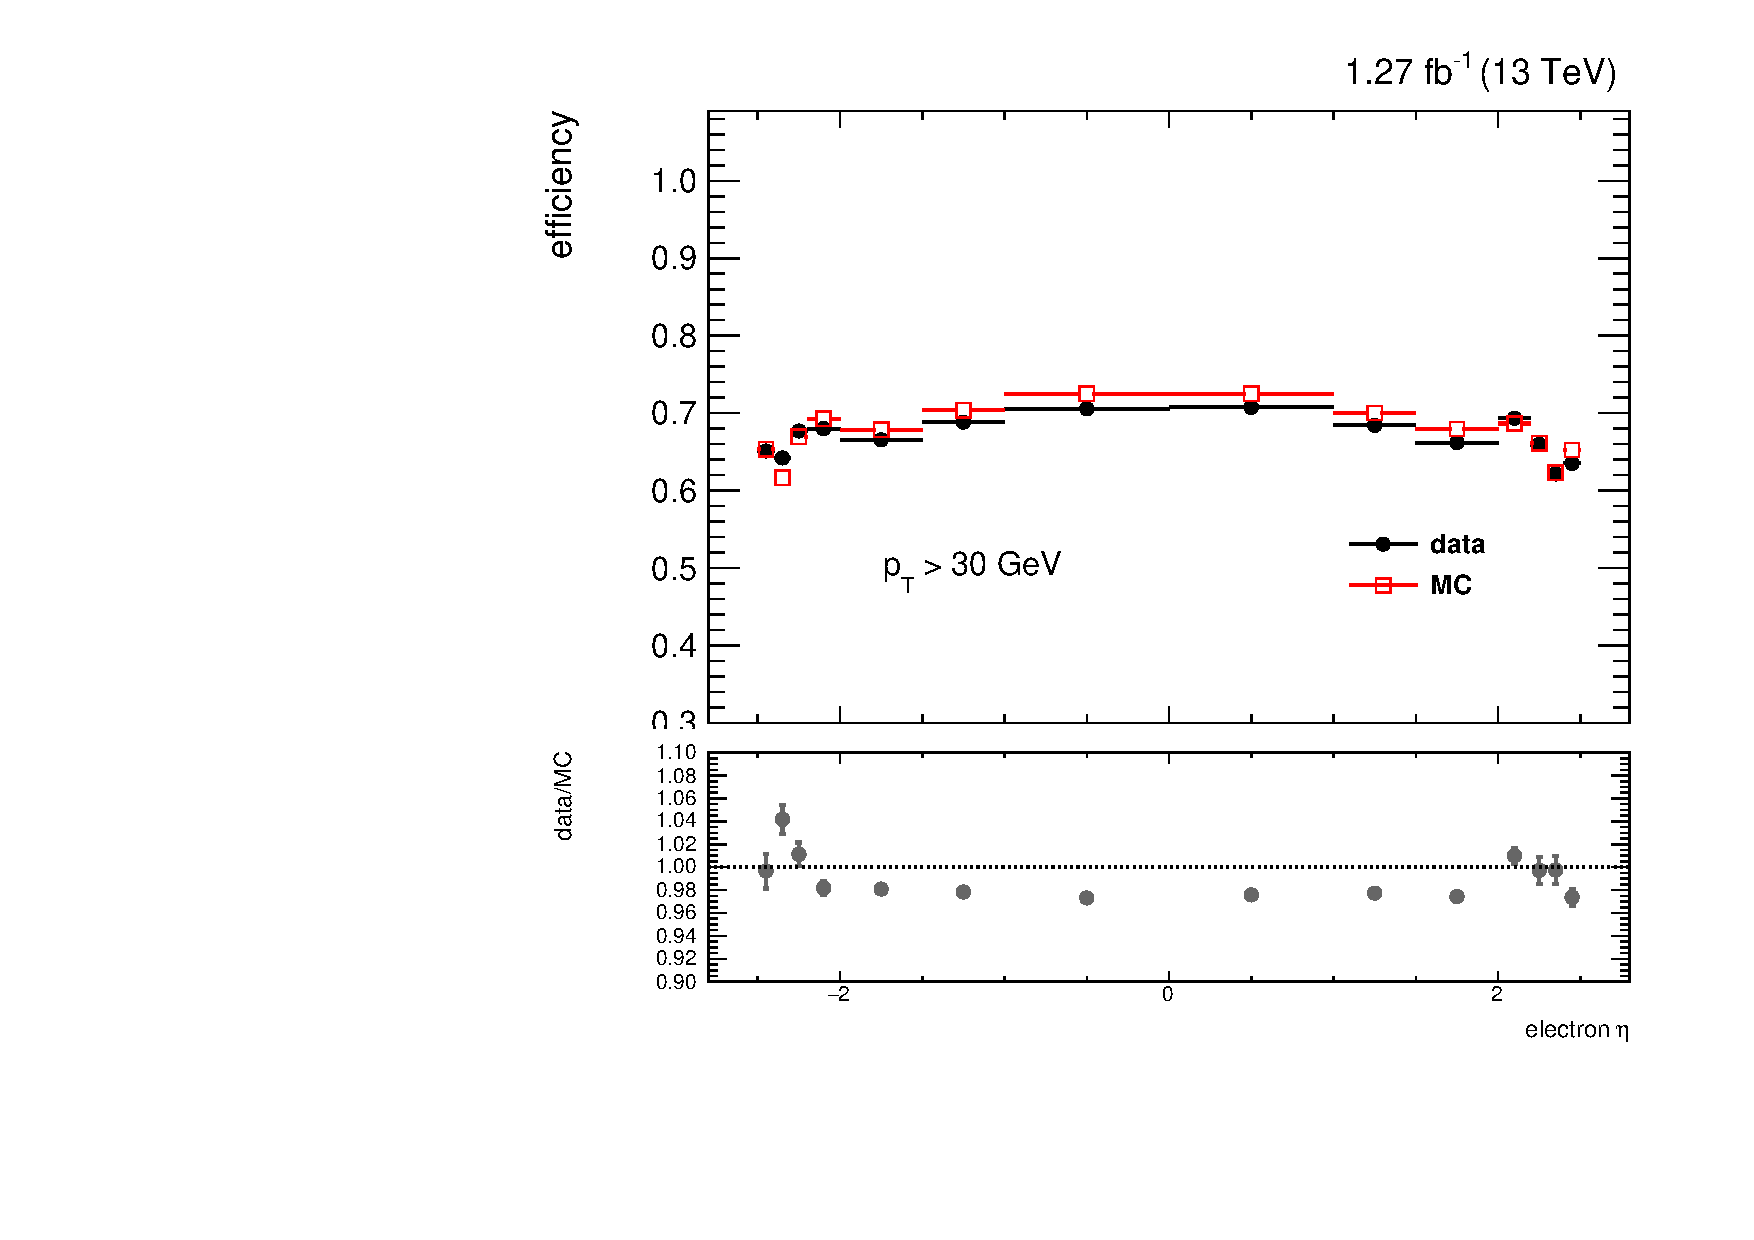
\includegraphics[width=0.48\textwidth]{figures/eltight_effeta_dataMC.pdf}}
  \subfigure[]{\label{subfig:eltighteffnpv}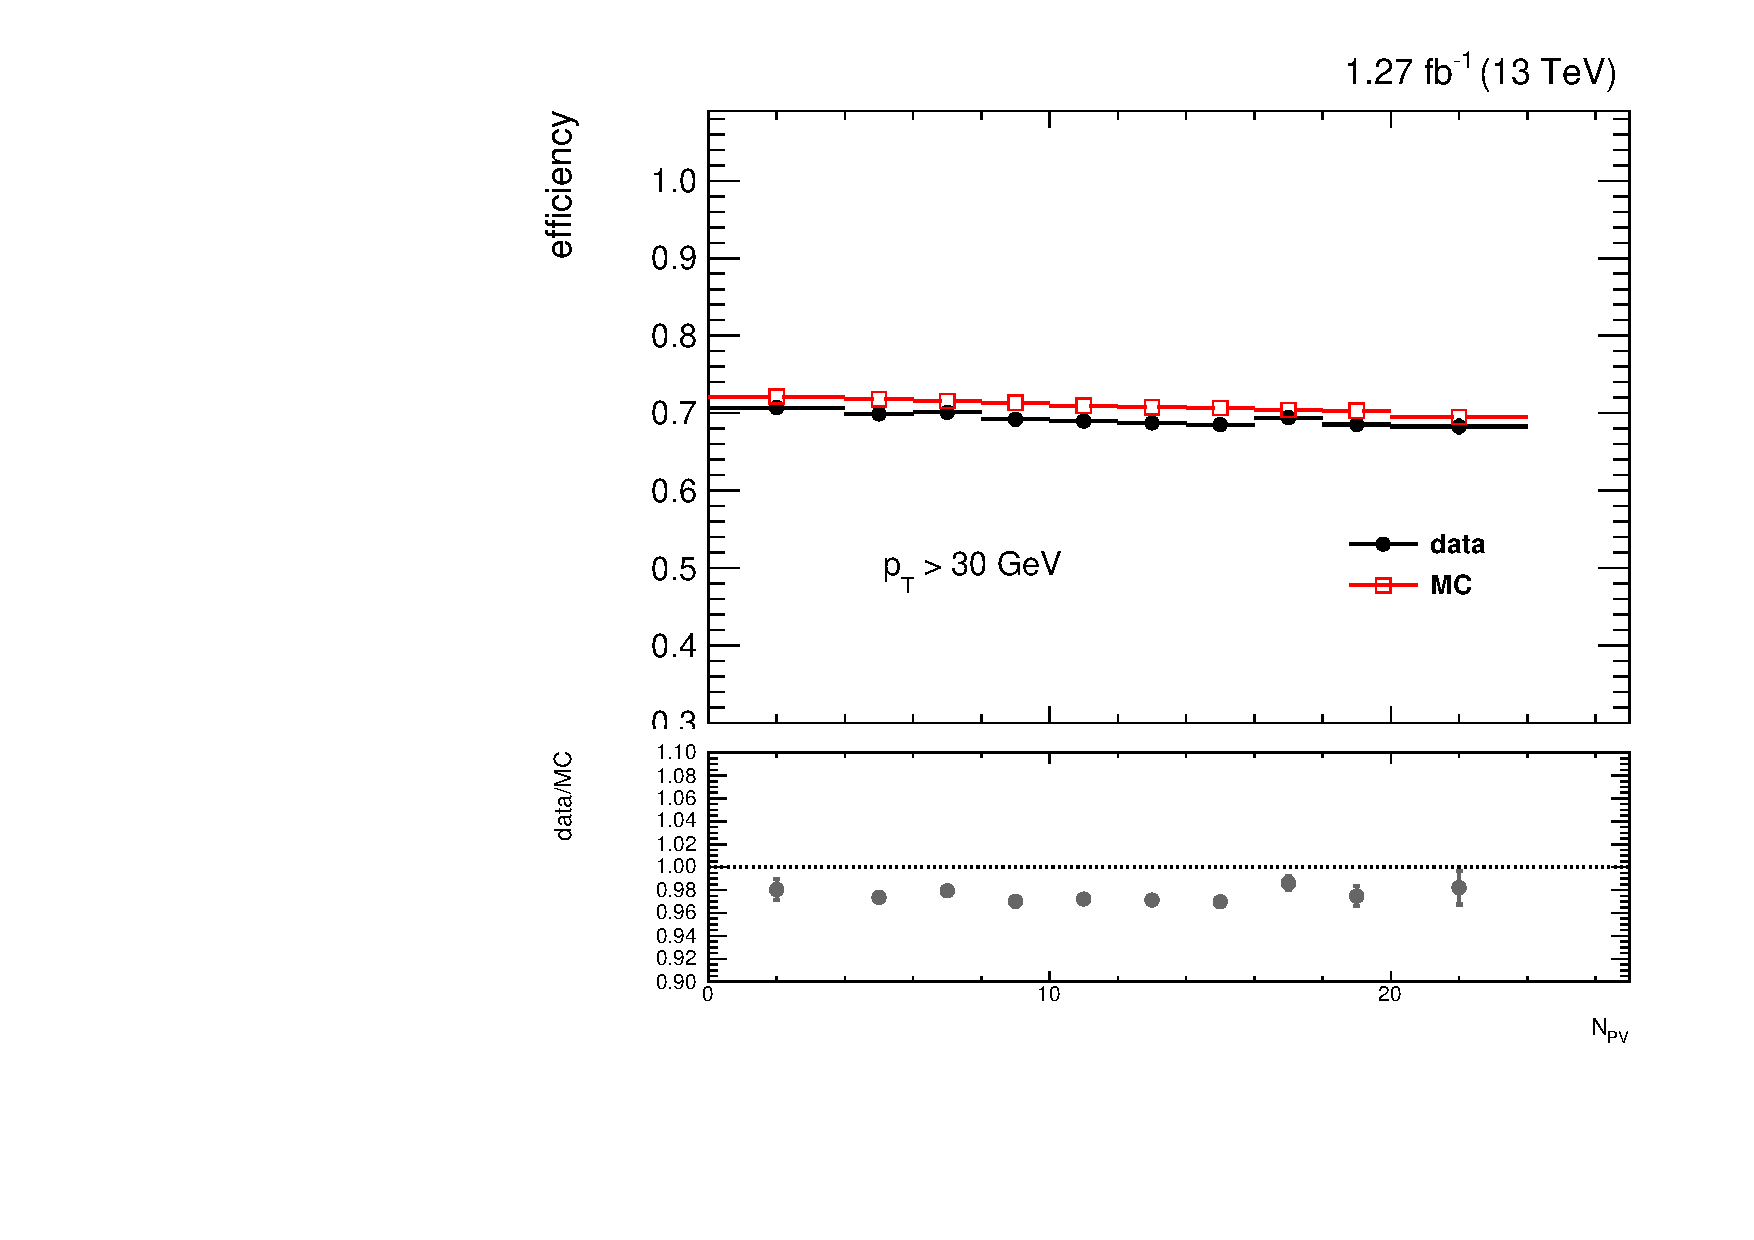
\includegraphics[width=0.48\textwidth]{figures/eltight_effnpv_dataMC.pdf}}
  \caption{Electron ``Tight'' WP efficiencies with respect to \subref{subfig:eltighteffeta} $\eta$ and \subref{subfig:eltighteffnpv} $N_{PV}$.}
  \label{fig:eltighteff}
\end{center}
\end{figure}

\subsection{Muons}
\label{subsec:obj_muon}


Muons are selected using the ``Tight'' and ``Loose'' offline cut-based definitions. Similar to electrons, ``Tight'' muons are used for semileptonic top-pair selection and ``Loose'' muons are used to veto events with extra muons. The variables and cuts defining the selections are listed in Table~\ref{tab:tightmuon}. PF-based isolation with $R=0.4$ and $\Delta\beta$ correction is used.

\begin{table}[!ht]
\centering
\begin{tabular}{|c|c|c|}
\hline
  Variable                                          & Loose WP & Tight WP \\
\hline
  PF-muon                                           & true     & true   \\
  global muon                                       & -        & true   \\
  global OR tracker muon                            & true     & -      \\
  $\chi^2/$ndof of global muon fit $<$              & -        & $10$   \\
  No. of muon chamber hit in global muon fit $\geq$ & -        & $1$    \\
  No. of muon stations with muon segments $\geq$    & -        & $2$    \\
  $|d_0|$ (cm) $<$                                  & -        & $0.2$  \\
  $|d_z|$ (cm) $<$                                  & -        & $0.5$  \\
  No. of pixel hits $>$                             & -        & $0$    \\
  No. of tracker layers with hits $>$               & -        & $5$    \\
  relative isolation $<$                            & $0.2$    & $0.12$ \\
\hline
\end{tabular}
\caption{Variables and thresholds that define ``Loose'' and ``Tight'' muons. ``-'' indicates the variable is not considered for that working point.}
\label{tab:tightmuon}
\end{table}

Muon selection efficiencies measured with the tag-and-probe method in data and in the Drell-Yan MC sample are shown in Fig.~\ref{fig:mulooseeff} and Fig.~\ref{fig:mutighteff}. The data-to-MC tight muon selection efficiency scale factors for muons with $\pt>30\:\GeV\:$ are computed in $\pt$-$|\eta|$ bins and are shown in Table~\ref{tab:mutight_sf} and Fig.~\ref{fig:mu_sf}. Scale factors for the loose muon selection are shown in Table~\ref{tab:muloose_sf} and Fig.~\ref{fig:mu_sf}, and computed down to the $10\:\GeV\: \pt$ range. The point with large uncertainty in the $100\:\GeV\: \pt$ bin is due to the small number of events contained in the MC failing ``probes" sample, with the negative weights causing an overall negative yield. We will proceed to handle this by specifying a minimum allowable yield of 0 events.


 \begin{table}[!ht]
 \centering
 \begin{tabular}{|c|c|c|c|}
 \hline
 &                          &                              &                           \\
 & $0.0 < |\eta| < 1.2$ & $1.2 < |\eta| < 2.1$ & $2.1 < |\eta| < 2.4$ \\
  &                          &                              &                           \\
 \hline
 $30 < \pt <  40$ &  $0.997 \pm  0.001$  &  $0.999 \pm  0.001$  &  $0.990 \pm  0.002$ \\
 \hline
 $40 < \pt <  50$ &  $0.994 \pm  0.001$  &  $0.995 \pm  0.001$  &  $0.991 \pm  0.002$ \\
 \hline
 $50 < \pt < 100$ &  $0.992 \pm  0.001$  &  $0.993 \pm  0.001$  &  $0.982 \pm  0.008$ \\
\hline
$100 < \pt < 150 $&  $0.985 \pm  0.005$  &  $0.986 \pm  0.006$  &  $1.001 \pm  0.017$ \\
 \hline
  $    \pt > 150$ &  $0.984 \pm  0.009$  &  $0.960 \pm  0.012$  &  $0.904 \pm  0.040$ \\
\hline
\end{tabular}
\caption{Tight muon selection efficiency scale factors for muons with $\pt>30\:\GeV\:$}
\label{tab:mutight_sf}
\end{table}

\begin{table}[!ht]
 \centering
 \begin{tabular}{|c|c|c|c|}
 \hline
 &                          &                              &                           \\
 & $0.0 < |\eta| < 1.2$ & $1.2 < |\eta| < 2.1$ & $2.1 < |\eta| < 2.4$ \\
  &                          &                              &                           \\
 \hline
 $10 < \pt <  15$ &  $1.012 \pm  0.012 $ &  $0.994 \pm  0.011$  &  $0.992 \pm  0.019$ \\
 \hline
 $15 < \pt<  20$ &  $0.982 \pm  0.007$  &  $0.981 \pm  0.007$  &  $0.993 \pm  0.013$ \\
 \hline
 $20 < \pt <  25$ &  $0.998 \pm  0.004$  &  $1.007 \pm  0.005$  &  $1.007 \pm  0.008$ \\
 \hline
 $25 <  \pt<  30$ &  $0.999 \pm  0.002$  &  $1.001 \pm  0.002$  &  $1.010 \pm  0.004$ \\
 \hline
 $30 < \pt<  40$ &  $1.002 \pm  0.001$  &  $1.002 \pm  0.001$  &  $1.001 \pm  0.001$ \\
 \hline
 $40 < \pt <  50$ &  $1.001 \pm  0.001$  &  $1.000 \pm  0.001$  &  $1.002 \pm  0.001 $\\
 \hline
 $50 <\pt < 100$ &  $1.000 \pm  0.001$  &  $0.999 \pm  0.001$  &  $1.001 \pm  0.001$ \\
 \hline
$100 < \pt< 150$ & $ 0.997 \pm  0.003$  &  $0.997 \pm  0.003$  &  $0.999 \pm  0.999$ \\
\hline
$\pt> 150$ &  $1.004 \pm  0.004$  &  $0.987 \pm  0.007 $ &  $1.000 \pm  0.008$ \\
\hline
\end{tabular}
\caption{Loose muon selection efficiency scale factors for muons with $\pt>10\:\GeV\:$}
\end{table}


\begin{figure}[htbp]
\begin{center}
  \subfigure[]{\label{sub fig:mutightsf}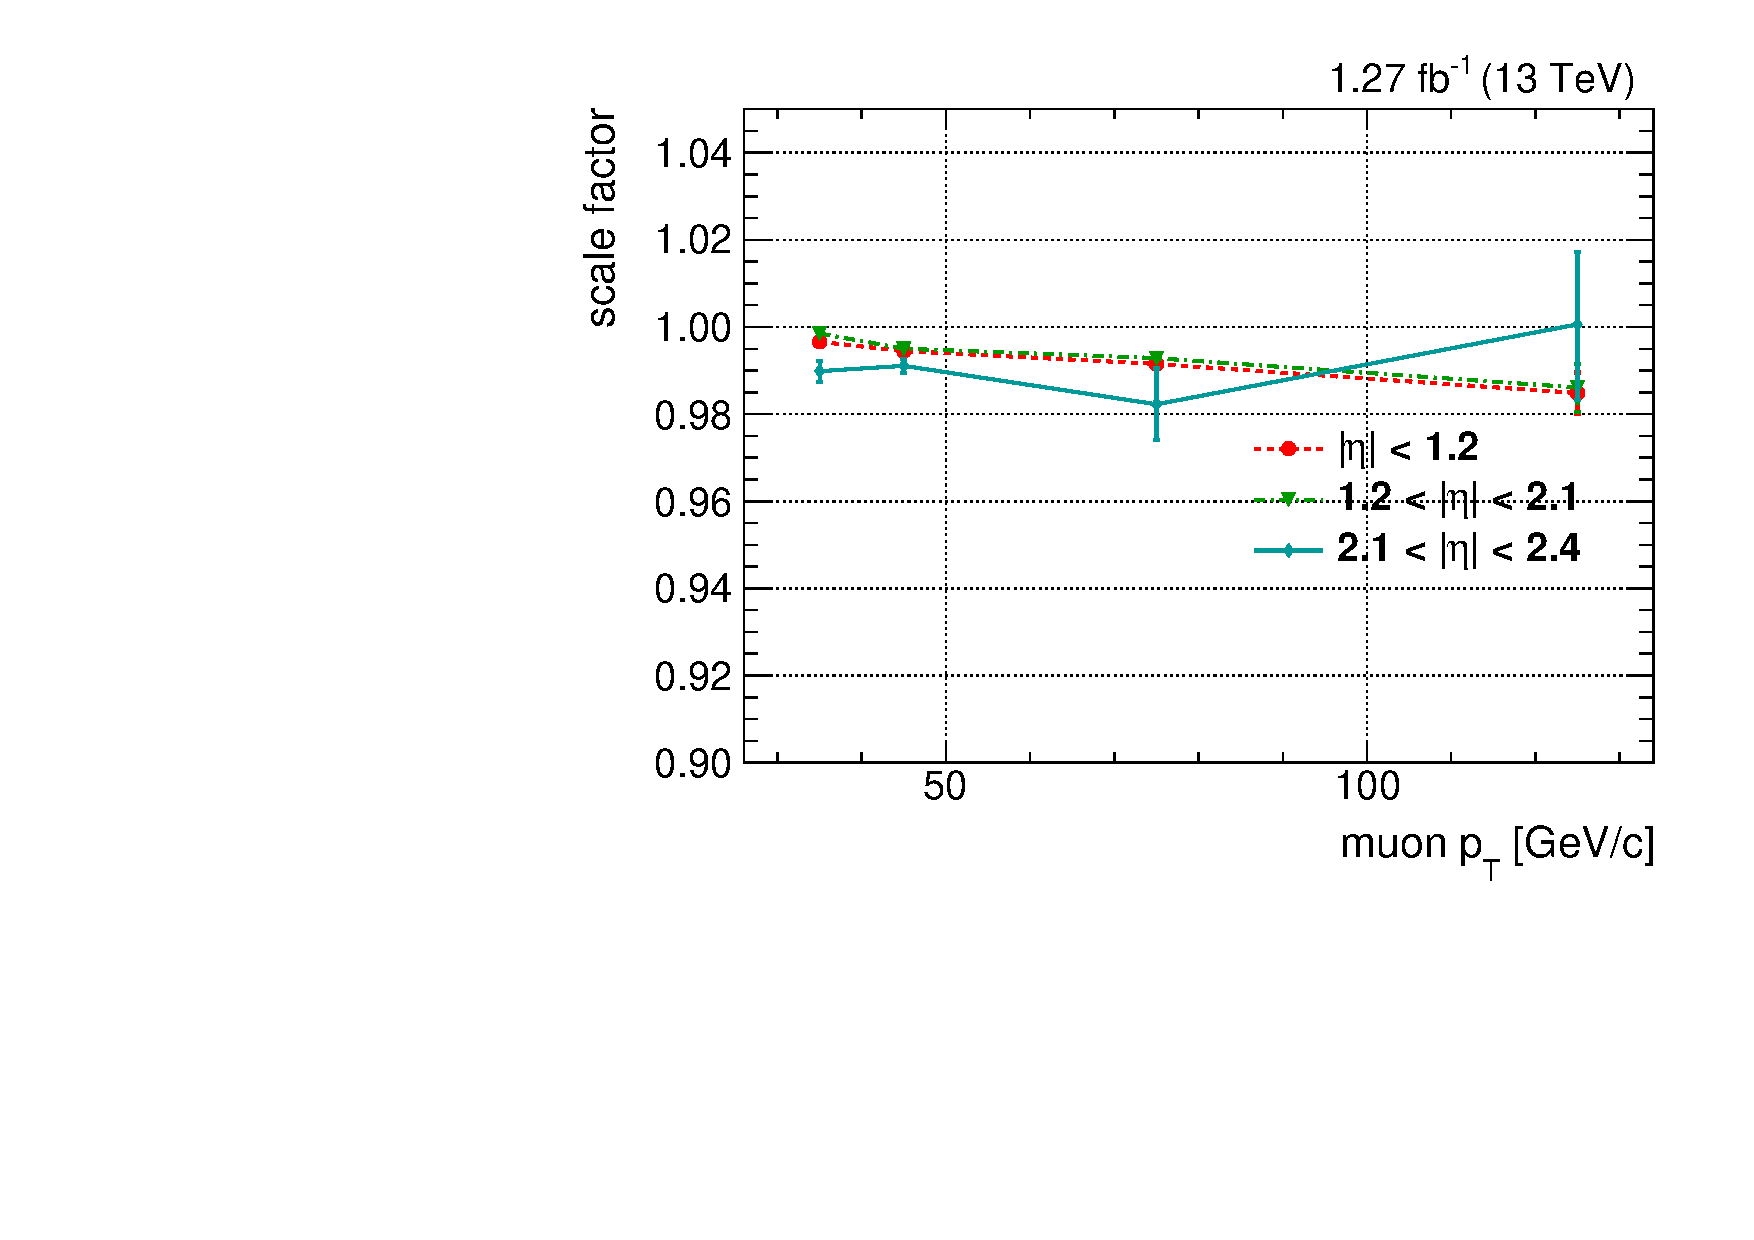
\includegraphics[width=0.48\textwidth]{figures/mutight_sfetapt.pdf}}	
  \subfigure[]{\label{sub fig:muloosesf}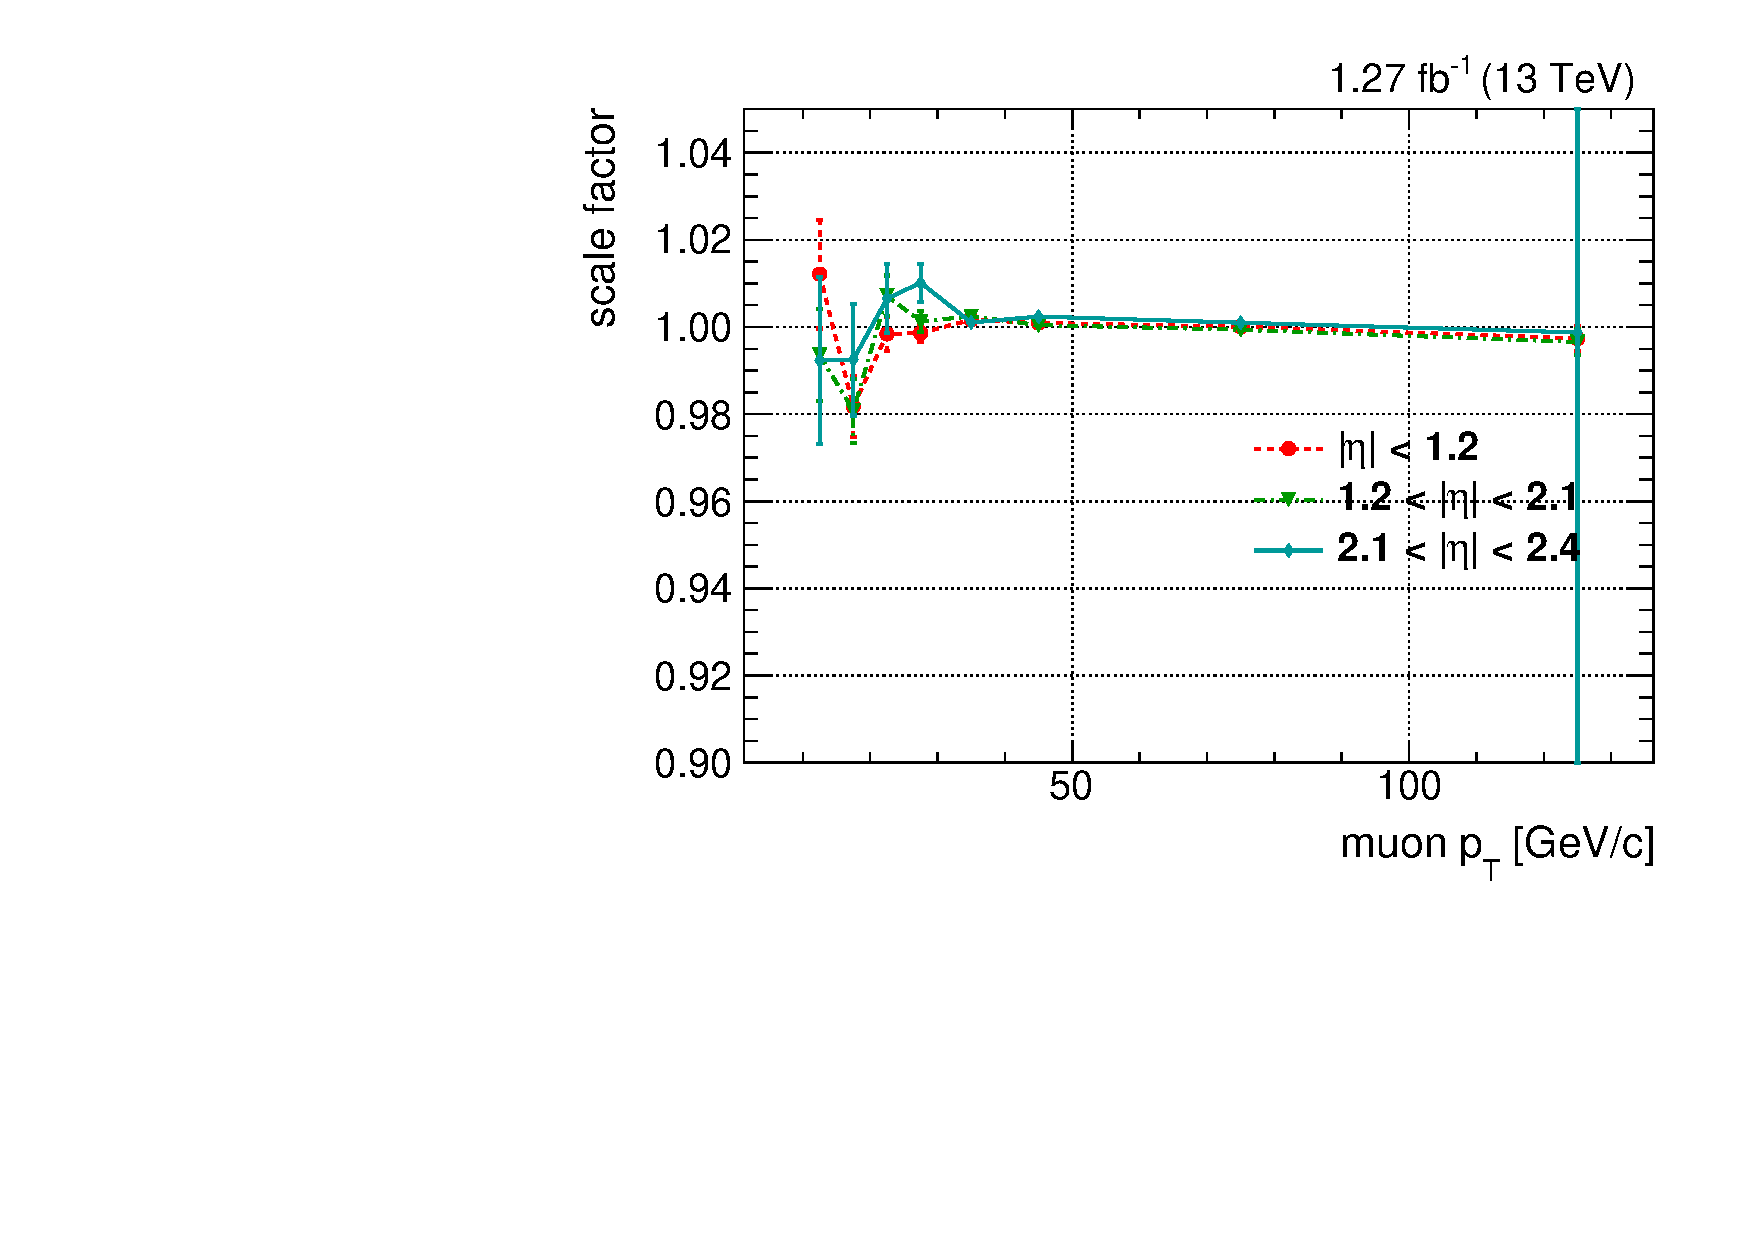
\includegraphics[width=0.48\textwidth]{figures/muloose_sfetapt.pdf}}
  \caption{Muon ``Tight" WP (left) and ``Loose" WP (right) data-to-MC efficiency scale factors as a function of muon $\pt$ for various $|\eta|$ bins.}
  \label{fig:mu_sf}
\end{center}
\end{figure}


\begin{figure}[htbp]
\begin{center}
  \subfigure[]{\label{subfig:mulooseeffeta}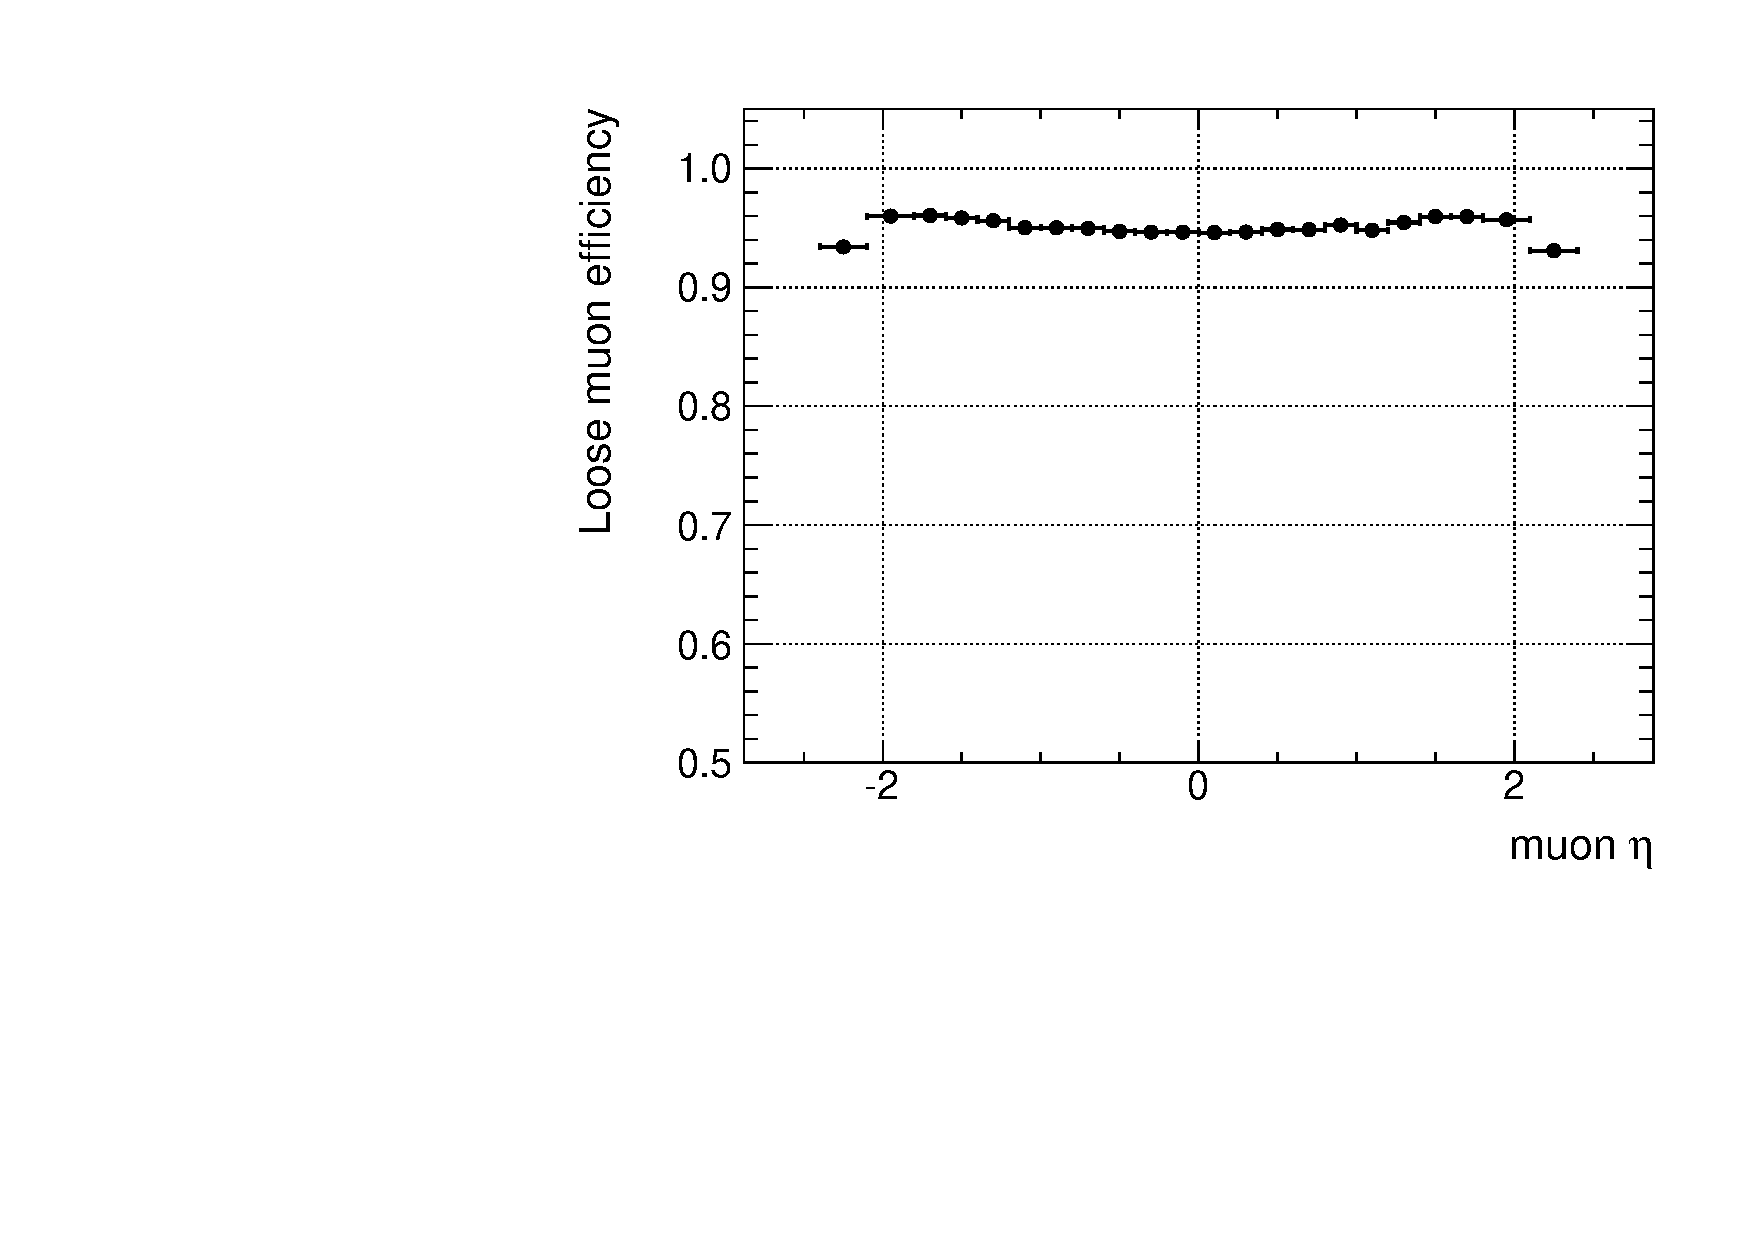
\includegraphics[width=0.48\textwidth]{figures/muloose_effeta.pdf}}
  \subfigure[]{\label{subfig:mulooseeffpt}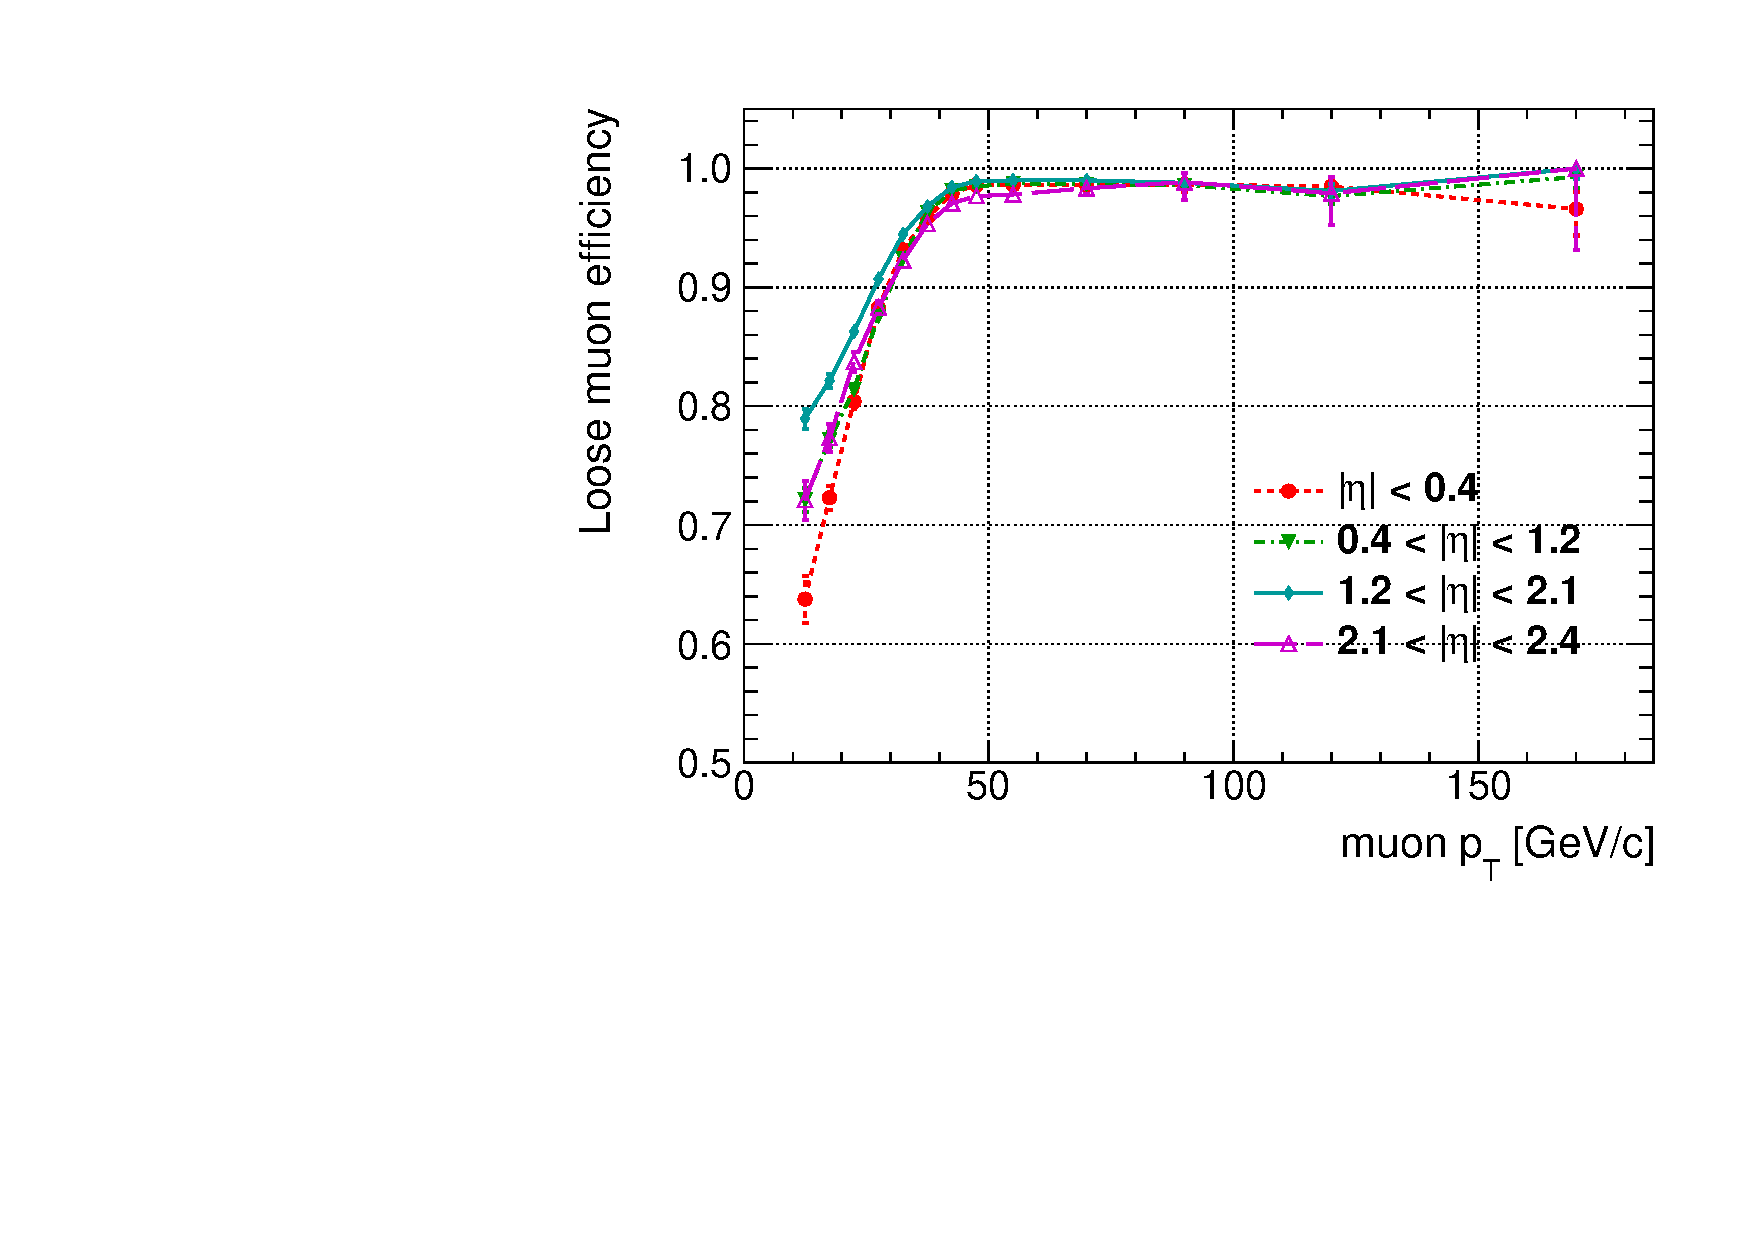
\includegraphics[width=0.48\textwidth]{figures/muloose_effetapt.pdf}}
  \caption{Muon ``Loose'' WP efficiencies with respect to \subref{subfig:mulooseeffeta} $\eta$ and \subref{subfig:mulooseeffpt} $\pt$ in different $|\eta|$-regions.\textcolor{red}{Plots to be updated}}
  \label{fig:mulooseeff}
\end{center}
\end{figure}

\begin{figure}[htbp]
\begin{center}
  \subfigure[]{\label{subfig:mutighteffeta}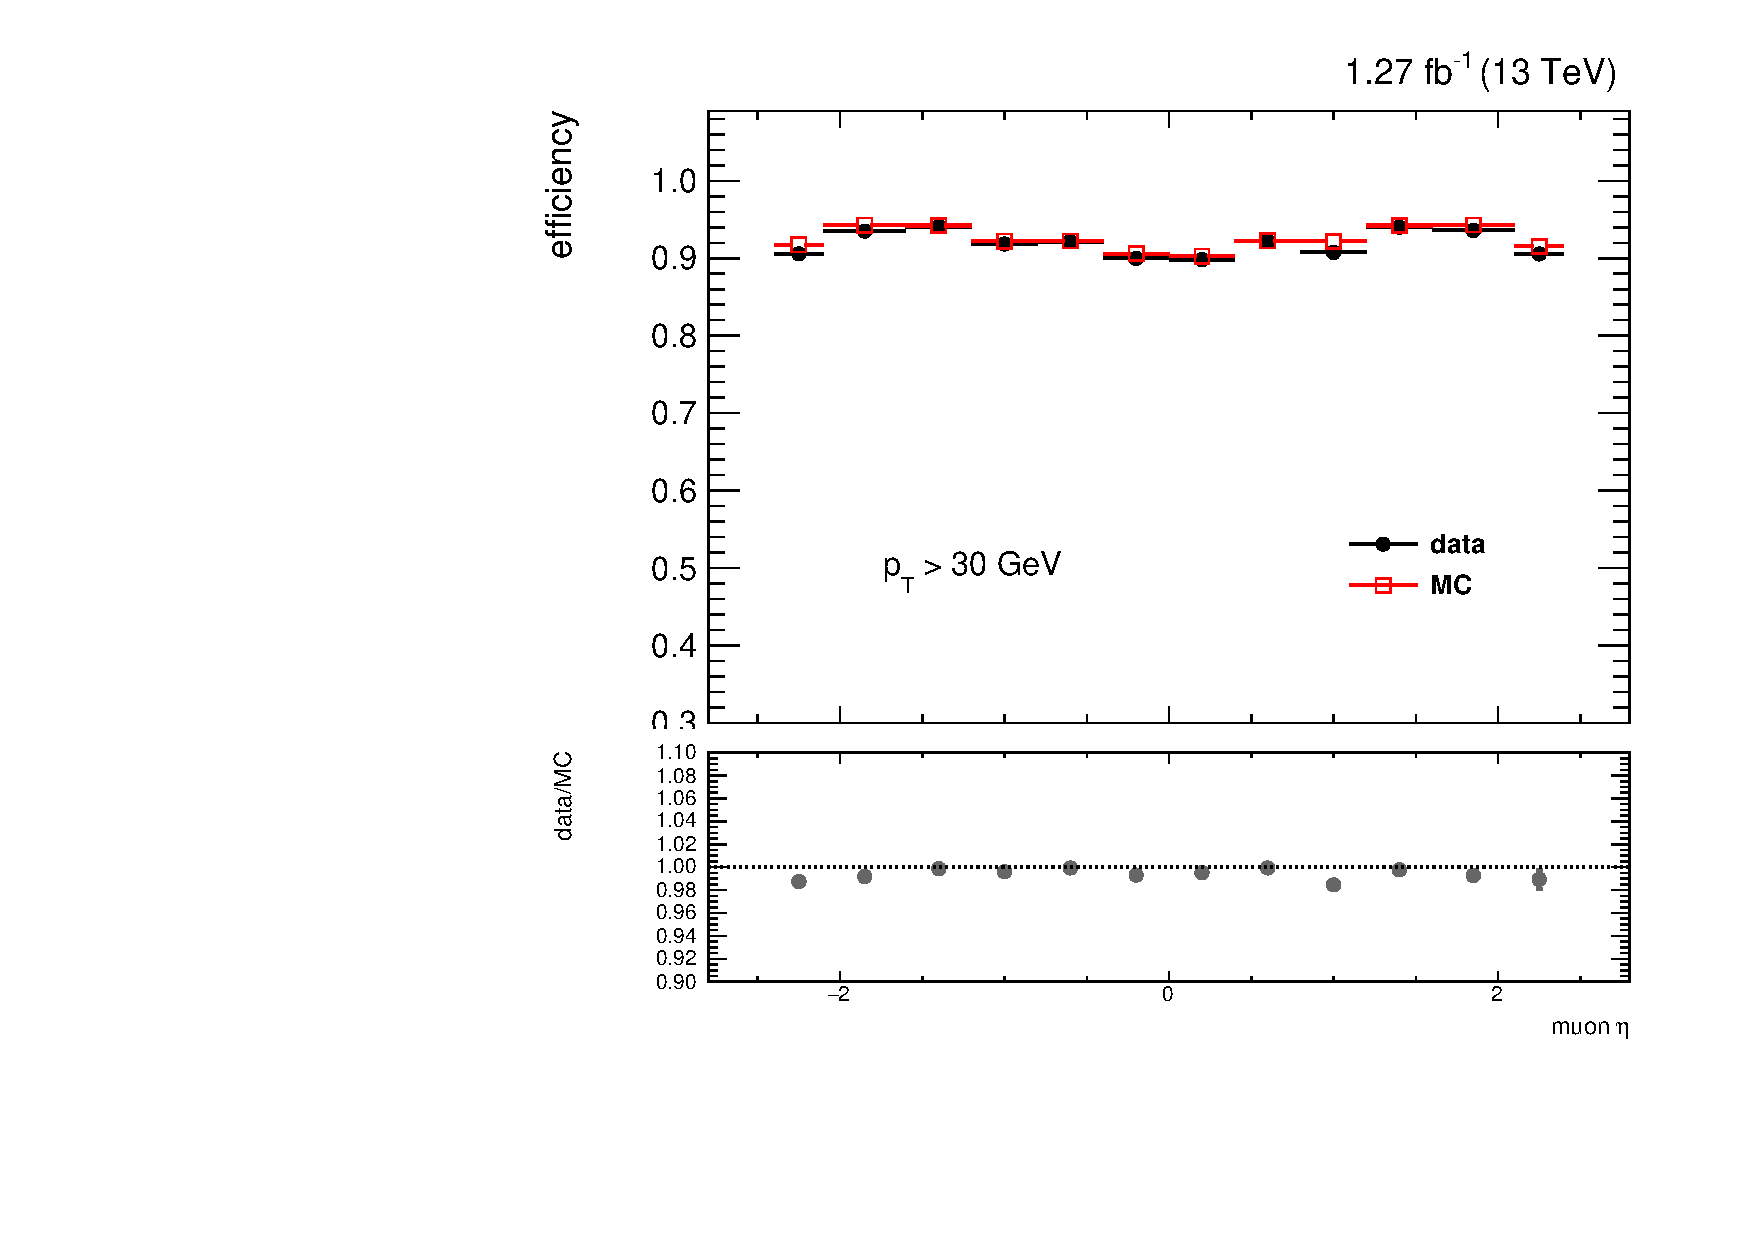
\includegraphics[width=0.48\textwidth]{figures/mutight_effeta_dataMC.pdf}}
  \subfigure[]{\label{subfig:mutighteffpt}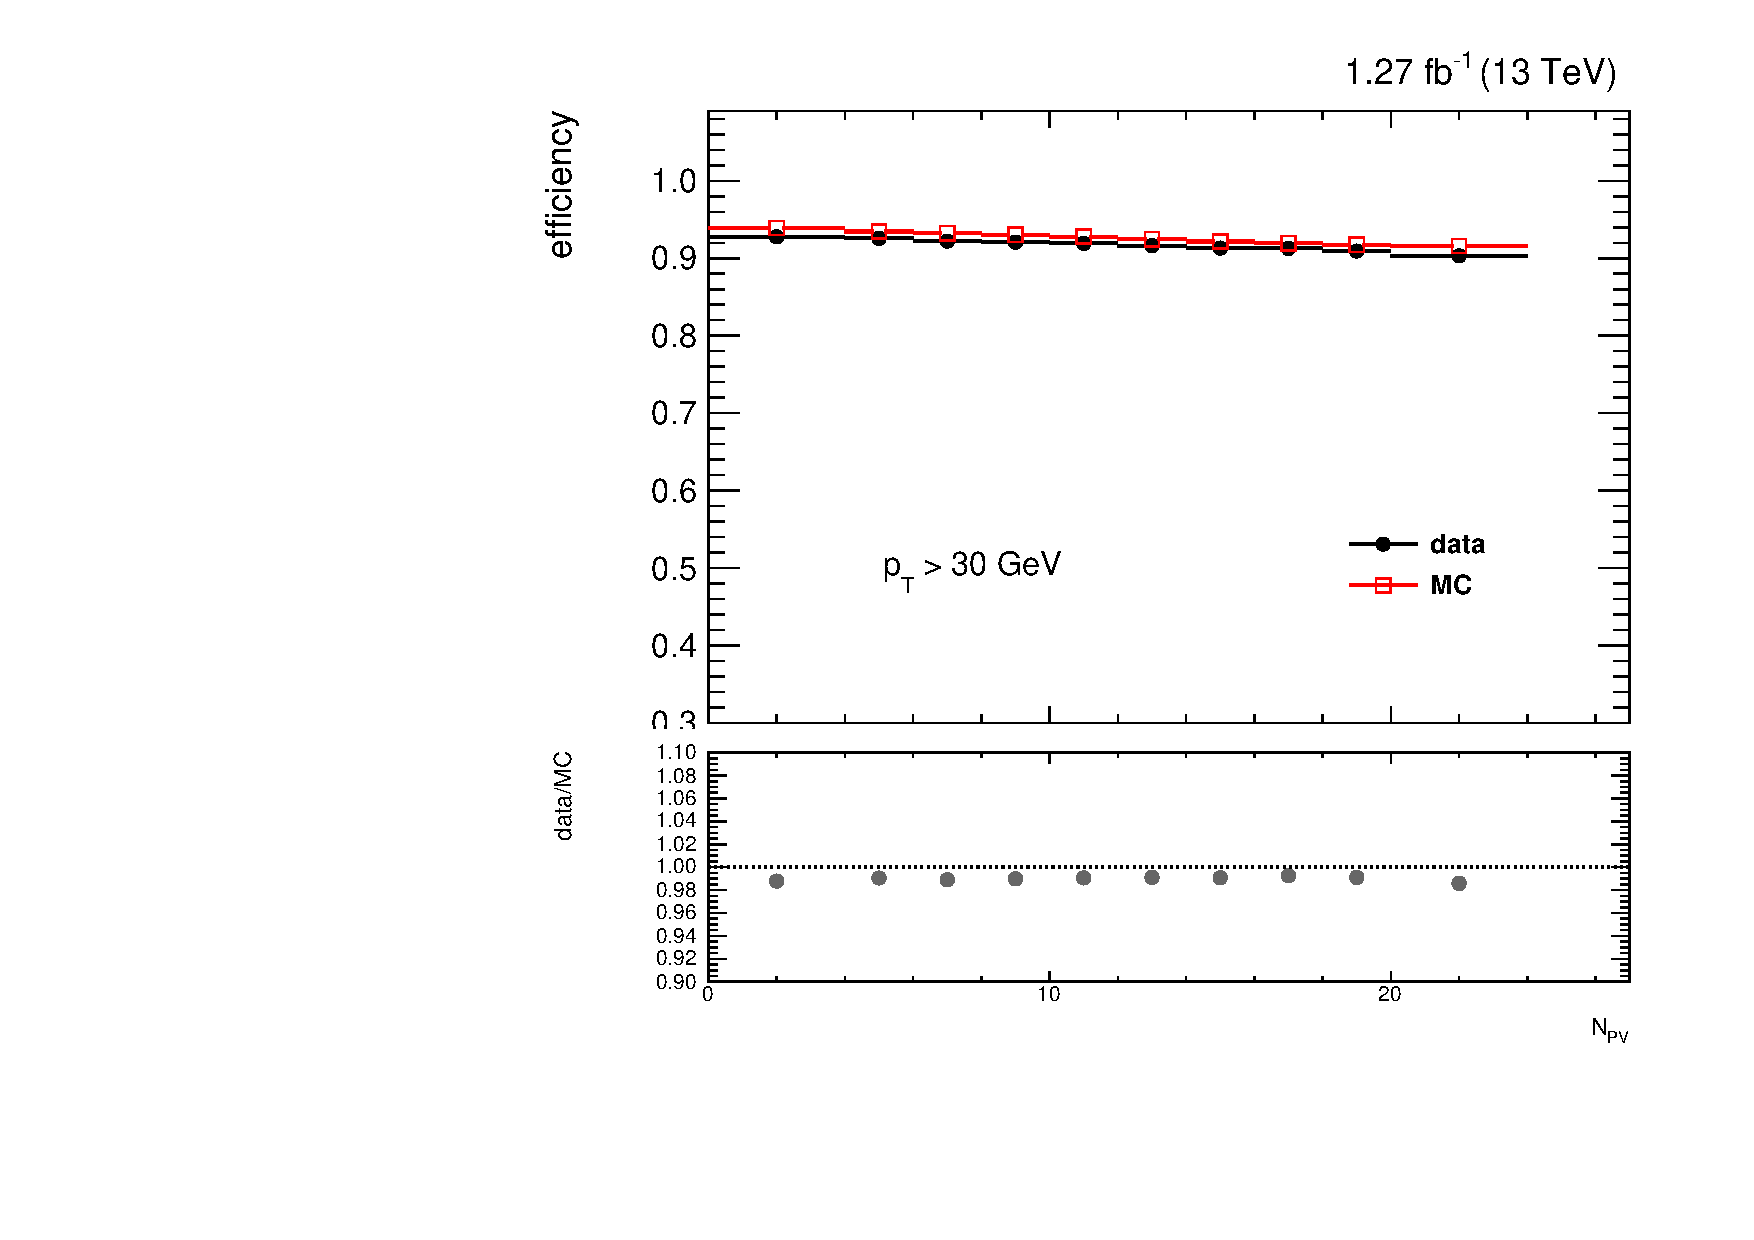
\includegraphics[width=0.48\textwidth]{figures/mutight_effnpv_dataMC.pdf}}
  \caption{Muon ``Tight'' WP efficiencies with respect to \subref{subfig:mutight_effeta_dataMC} $\eta$ and \subref{subfig:mutight_effnpv_dataMC} $N_{PV}$ in data and MC for muons with $\pt>30\:\GeV\:$.}
  \label{fig:mutighteff}
\end{center}
\end{figure}

\clearpage
%\input{obj_tau}
\subsection{Jets}
\label{subsec:obj_jets}

Jets are reconstructed by clustering PF-candidates. The jet collection used in this analysis are clustered with the anti-$k_T$ algorithm with size parameter, $R=0.4$. This jet collection employs charged hadron subtraction (CHS) to reduce pileup contamination. The anti-$k_T$ collection will be denoted as \emph{AK4CHS}. Jets must pass the ``Loose PF Jet ID'' requirements listed in Table~\ref{tab:jetid}.  %Two jet collections are used in this analysis: jets from clustering with the anti-$k_T$ algorithm with size parameter, $R=0.4$, and jets from clustering with the Cambridge-Aachen (CA) algorithm with $R=1.5$. The collection of $R=1.5$ jets are used to tag boosted, hadronically decaying tops by applying jet substructure techniques. Both jet collections employ charged hadron subtraction (CHS) to reduce pileup contamination. The anti-$k_T$ and CA jet collections will be denoted as \emph{AK4CHS} and \emph{CA15CHS} respectively. Jets from either collection must pass the ``Loose PF Jet ID'' requirements listed in Table~\ref{tab:jetid}.

\begin{table}[!ht]
\centering
\begin{tabular}{|c|c|}
\hline
  Variable                     &  Threshold \\
\hline
  Neutral Hadron Fraction $<$  & $0.99$     \\
  Neutral EM Fraction $<$      & $0.99$     \\
  Number of Constituents $>$   & $1$        \\
  %Muon Fraction $<$            & $0.8$      \\
\hline
  \multicolumn{2}{|c|}{\emph{Additional cuts for $|\eta|<2.4$}} \\
\hline
  Charged Hadron Fraction $>$  & $0$        \\
  Charged Multiplicity $>$     & $0$        \\
  Charged EM Fraction $<$      & $0.99$     \\
\hline
\end{tabular}
\caption{Variables and thresholds that define the ``Loose PF Jet ID''.}
\label{tab:jetid}
\end{table}

Standard jet energy corrections (JEC), corresponding to the official Run 2 V5 global tag, are applied. %In the case of CA15CHS jets, the JEC for anti-$k_T$ $R=0.8$ jets with CHS are used because this is the largest size parameter with corrections available.

To tag jets that originate from $\Bot$-quarks, the \emph{CSVv2+IVF} discriminator is used with the recommended medium working point. An AK4CHS jet is considered a $\Bot$-jet if $\mbox{CSVv2+IVF} > 0.814$.

\subsection{\texorpdfstring{$\met$}{MET}}
\label{subsec:obj_met}

The missing transverse energy ($\met$) is computed from the negative vector sum of momenta over all PF-candidates. The ``Type-1'' correction is applied, which accounts for the JEC.

Differences in the calorimeter response to hadronic activity between simulation and data accounts for much of the difference in $\met$ scale and resolution between MC and data. A residual correction to $\met$ can be derived by calibrating the response and resolution of the hadronic recoil using $\Zjets$ and $\gamma+$jets events data \cite{recoil}. The distributions of the recoil components (parallel and perpendicular to the boson $\pt$ direction) are fit and subsequently polynomials are fit to the extracted mean and width of the recoil distributions as functions of the boson $\pt$. The mean resolutions of the parallel and perpendicular components are shown in Fig.~\ref{fig:met_MR}.


\begin{figure}[htbp]
\centering
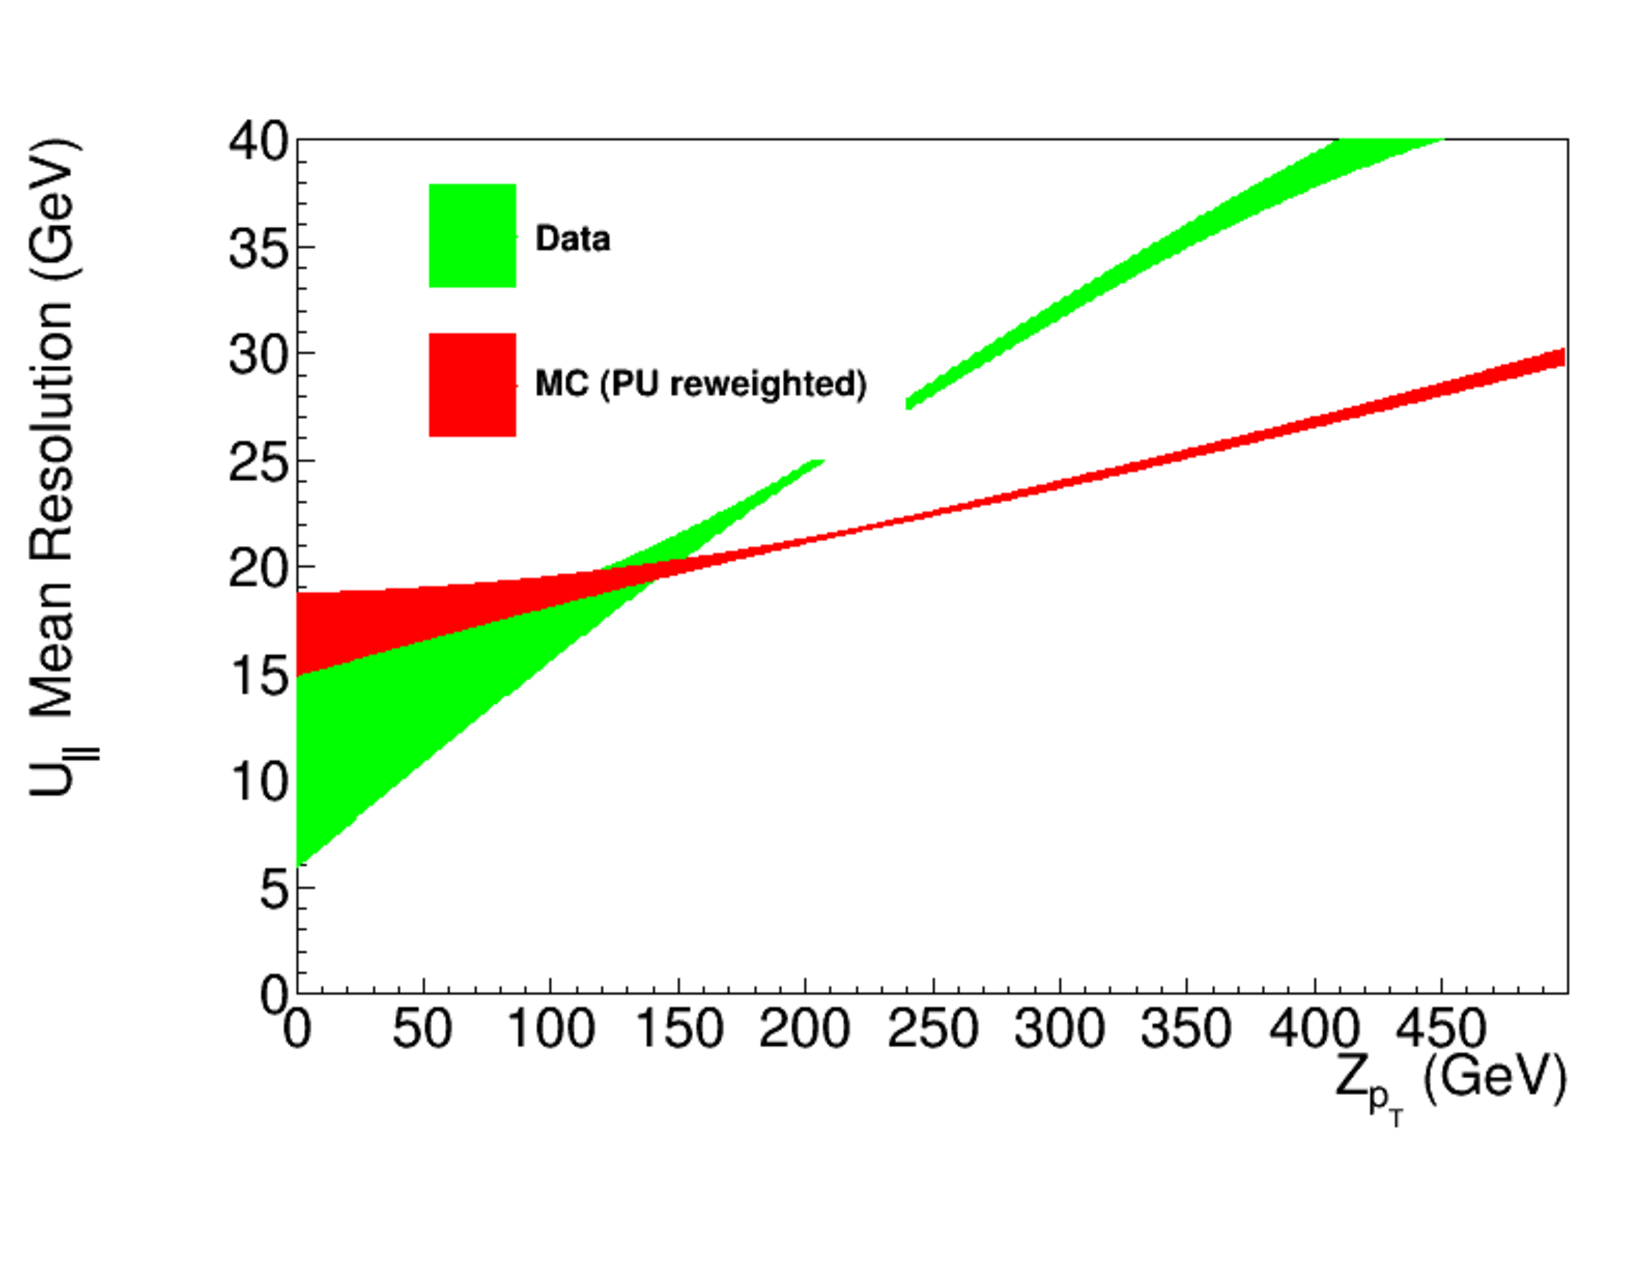
\includegraphics[width=0.48\textwidth]{figures/u1MR.pdf}
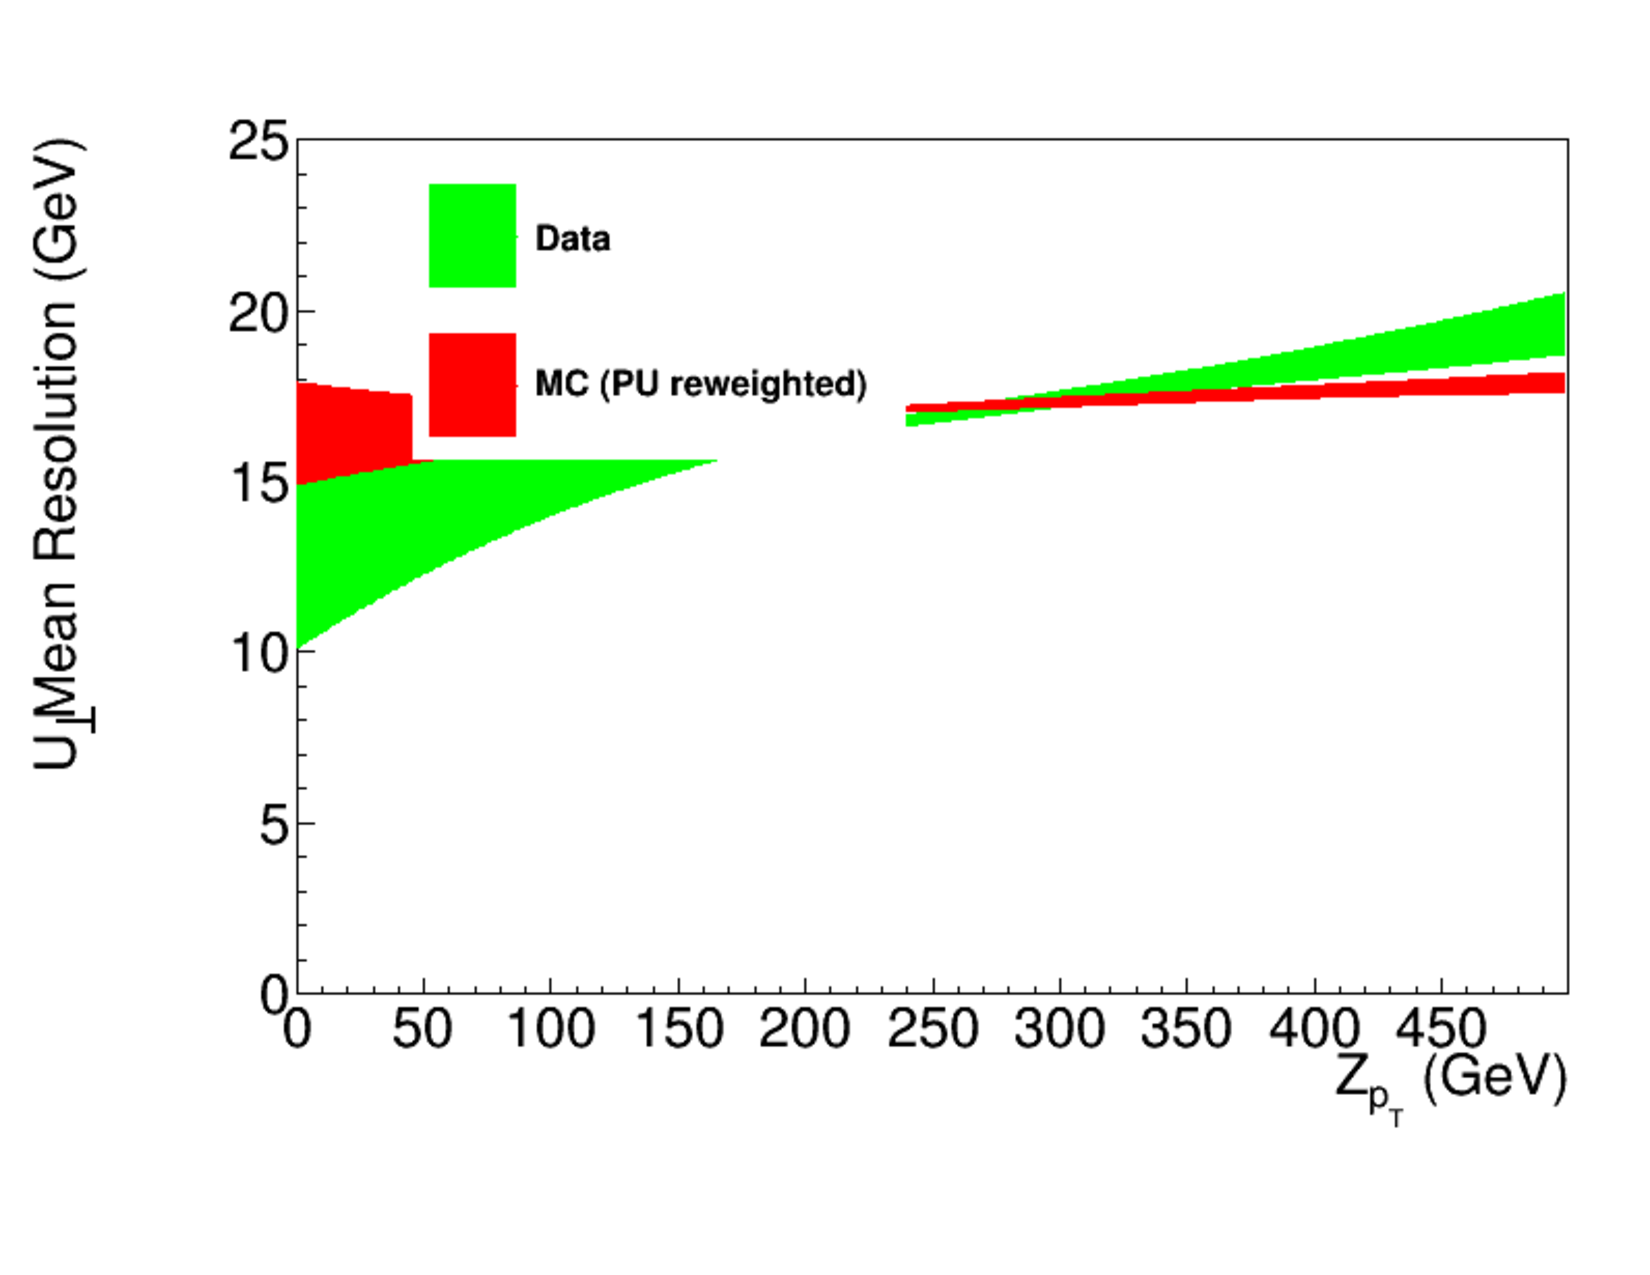
\includegraphics[width=0.48\textwidth]{figures/u2MR.pdf}
\caption{Mean resolution of hadronic recoil components that are parallel (left) and perpendicular (right) to boson $\pt$ in $\Zjets$ and $\gamma+$jets data and MC events.}
\label{fig:met_MR}.
\end{figure}



\subsection{Photons}
\label{subsec:obj_photon}

Photons are selected to obtain a control sample to model the $\Z\To\Nu\Nu$ background. A cut-based selection at the ``Medium'' WP from the ``V2'' prescriptions derived from Phys14 samples is used; the variables and cuts are described in Table~\ref{tab:photon_id}. Isolation quantities are computed from PF-candidates within a cone of $R=0.3$ around the photon. The pileup contribution to each type of isolation quantity is estimated by multiplying the effective area, $A_{\mbox{\scriptsize{eff}}}$, with the energy density, $\rho$, where $\rho$ is assigned to the quantity called, ``fixedGridRhoFastjetAll''. The effective areas are $\eta$-dependent and are listed in Table~\ref{tab:effarea}. For each type of isolation, the pileup corrected isolation is,
\begin{equation}
  I'_{k} = \max\left(I_k - A_{\mbox{\scriptsize{eff}},k}\cdot\rho, 0\right),
\end{equation}
where the $k$ index denotes $h^+$, $h^0$, or $\gamma$.

\begin{table}[!ht]
\centering
\begin{tabular}{|c|c|c|c|c|}
\hline
  Variable                              & Barrel                                            & Endcap \\
\hline
  single tower $H/E <$                  & $0.012$                                           & $0.023$  \\
  $\sigma_{i\eta i\eta} <$              & $0.0100$                                          & $0.0267$ \\
  charged hadron isolation (\GeV) $<$   & $1.79$                                            & $1.09$ \\
  neutral hadron isolation (\GeV) $<$   & $0.16 + \exp\left(0.0028\cdot\pt + 0.5408\right)$ & $4.31+0.0172\cdot\pt$ \\
  photon isolation (\GeV) $<$           & $1.90+0.0014\cdot\pt$                             & $1.90+0.0091\cdot\pt$ \\ 
\hline
\end{tabular}
\caption{Variables and thresholds that define ``Medium'' photons in the Phys14 ``V2'' cut-based selections. A photon is in the barrel if it has supercluster $|\eta|<1.479$, otherwise it is in the endcap.}
\label{tab:photon_id}
\end{table}

\begin{table}[!ht]
\centering
\begin{tabular}{|rcl|c|c|c|}
\hline
                          &&& $h^+$    & $h^0$    & $\gamma$ \\
\hline
 $0     \leq$ & $|\eta_{\mbox{\scriptsize{SC}}}|$ & $< 1$     & $0.0234$ & $0.0053$ & $0.0780$ \\
 $1     \leq$ & $|\eta_{\mbox{\scriptsize{SC}}}|$ & $< 1.479$ & $0.0189$ & $0.0103$ & $0.0629$ \\
 $1.479 \leq$ & $|\eta_{\mbox{\scriptsize{SC}}}|$ & $< 2$     & $0.0171$ & $0.0057$ & $0.0264$ \\
 $2     \leq$ & $|\eta_{\mbox{\scriptsize{SC}}}|$ & $< 2.2$   & $0.0129$ & $0.0070$ & $0.0462$ \\
 $2.2   \leq$ & $|\eta_{\mbox{\scriptsize{SC}}}|$ & $< 2.3$   & $0.0110$ & $0.0152$ & $0.0740$ \\
 $2.4   \leq$ & $|\eta_{\mbox{\scriptsize{SC}}}|$ & $< 2.4$   & $0.0074$ & $0.0232$ & $0.0924$ \\
 $2.4   \leq$ & $|\eta_{\mbox{\scriptsize{SC}}}|$ &           & $0.0035$ & $0.1709$ & $0.1484$ \\
\hline
\end{tabular}
\caption{Effective areas for pileup mitigation in the Phys14 ``V2'' cut-based isolation for photons.}
\label{tab:effarea}
\end{table}


\clearpage

\section{Event Selection}
\label{sec:selection}

Events with signatures consistent with $\ttbar$ production and large $\met$ are selected. An excess in the tails of the $\met$ distribution over SM expectations could indiciate the production of DM particles. Two final states have been studied,
\begin{itemize}
\item \textbf{Hadronic:} jets$+\met$ final state where the $\W$ daughters from the tops decay hadronically,
\item \textbf{Semileptonic:} $\Lep+$jets$+\met$ final state where one of the $\W$ daughters from the tops decay leptonically into a muon or electron and neutrino.
\end{itemize}

%Recent developments in jet substructure have established effective techniques for identifying highly boosted $\Top$ quarks that decay hadronically such that all decay products fall within a single jet. This allows definitions of signal region categories with higher purity in the kinematic regime of boosted tops. Therefore, two general selection strategies are presented:
Two exclusive categories are presented:
\begin{itemize}

\item \textbf{Inclusive:} a single signal category that does not target any kinematic region in particular.
\item \textbf{Top-tagged:} the signal region is comprised of resolved top tags.%divided into several categories based on the number of boosted top tags.
\end{itemize}

\subsection{Inclusive Selection: Hadronic channel}
\label{subsec:sel_incl_hadronic}
%\textcolor{red}{To be updated from Phys14 to Spring15 studies before full stats}
Events for the hadronic channel are obtained with two triggers. For events from runs before 254227, the trigger used is HLT\_PFMET170\_NoiseCleaned\_PFMHTNoMu120\_IDTight, while for subsequent runs, the trigger is HLT\_PFMETNoMu120\_JetIdCleaned\_PFMHTNoMu120\_IDTight. The efficiency of these triggers with respect to offline $\met$ in the single electron and single muon channels is shown in Fig.~\ref{fig:meteff_0}. Discrepancies in the turn-on curves between the two channels are under investigation. Overall efficiencies at the plateau in both channels are in agreement between data and MC (comparing the fit parameter $\epsilon_{0}$ and the fit).This dictates the use of a unity scale factor for data-to-MC $\met$ corrections.

\begin{figure}[htbp]
\centering
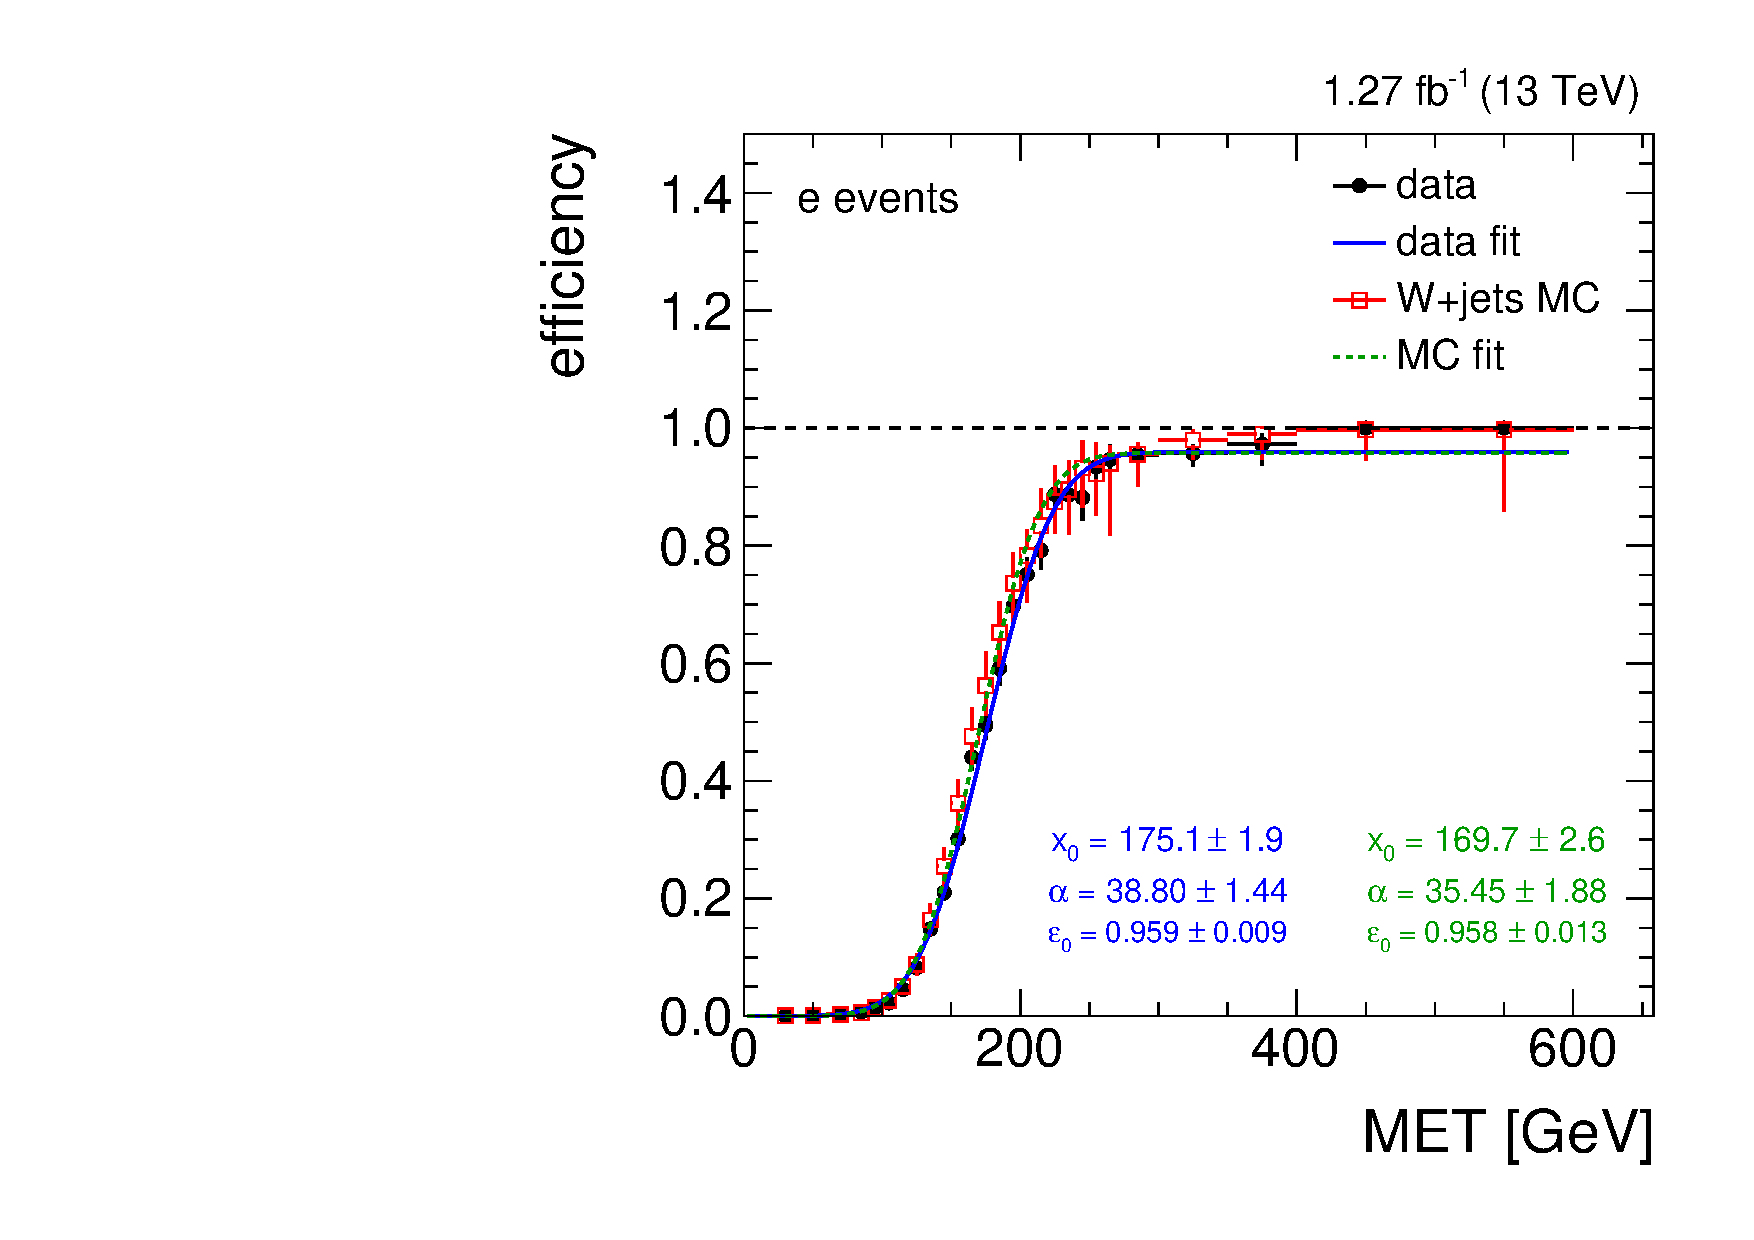
\includegraphics[width=0.48\textwidth]{figures/meteff_e_1.pdf}
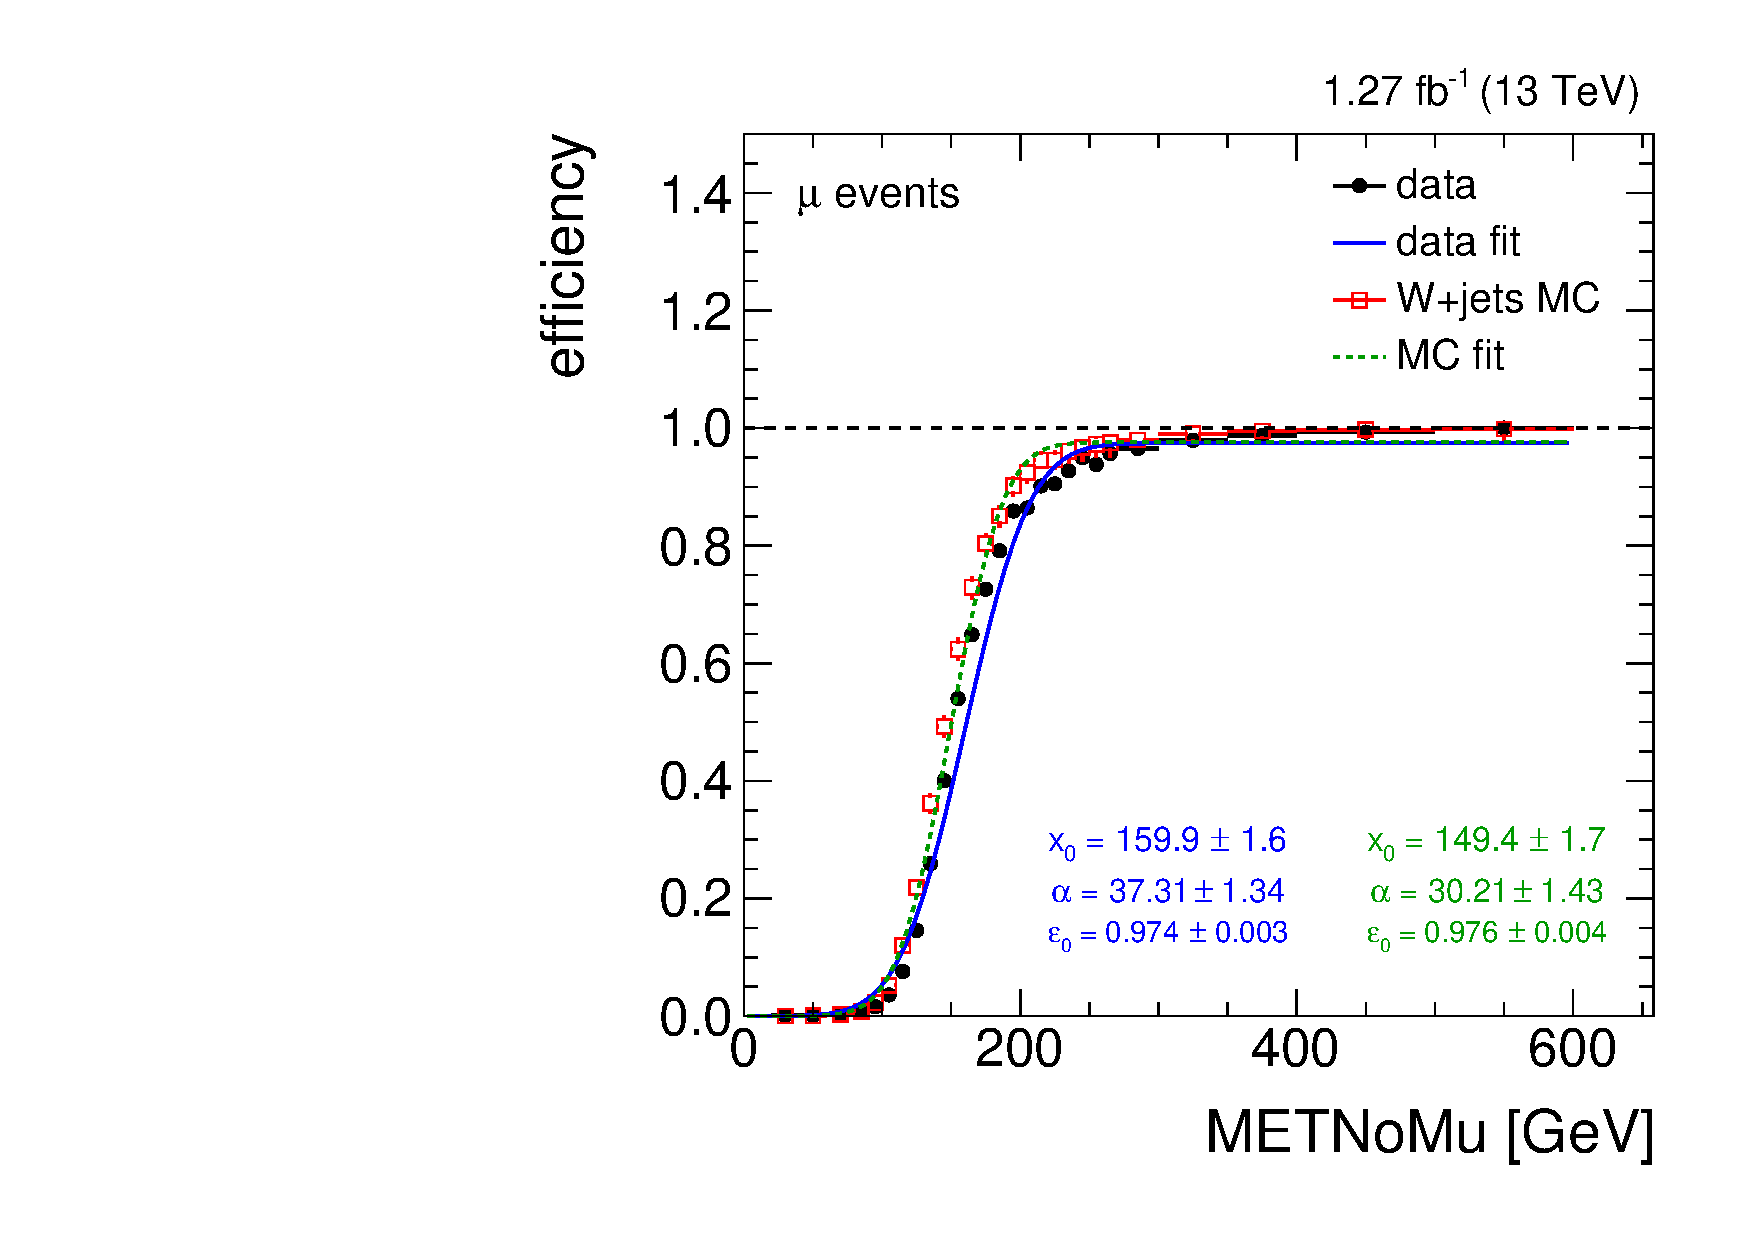
\includegraphics[width=0.48\textwidth]{figures/meteff_m_1.pdf}
\caption{Efficiency turn-on curves of HLT\_PFMET170\_NoiseCleaned\_PFMHTNoMu120\_IDTight and HLT\_PFMETNoMu120\_JetIdCleaned\_PFMHTNoMu120\_IDTight for electron events (left) and muon events (right). Events are required to have at least four jets.}
\label{fig:meteff_0}
\end{figure}

\begin{figure}[htbp]
  \centering
  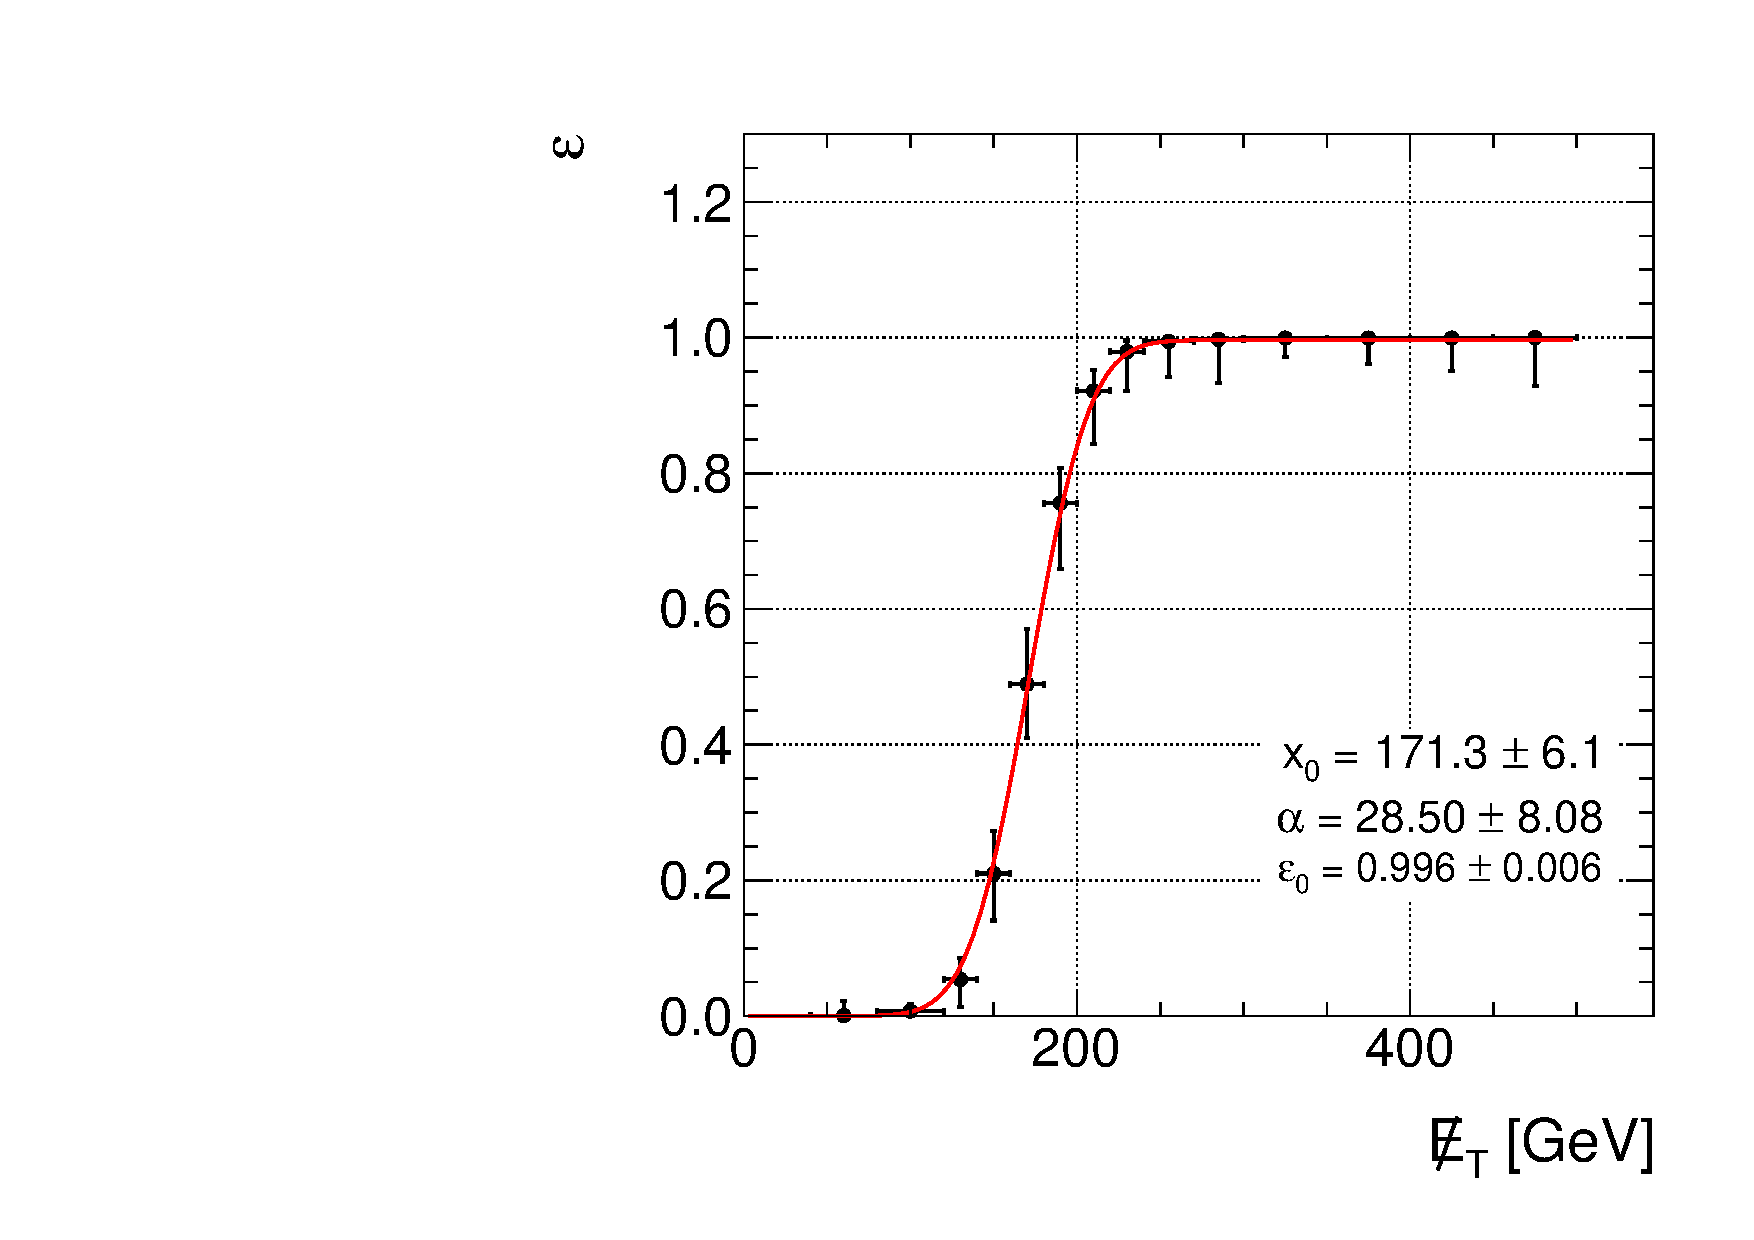
\includegraphics[width=0.48\textwidth]{figures/ttdm1-meteff.pdf}
  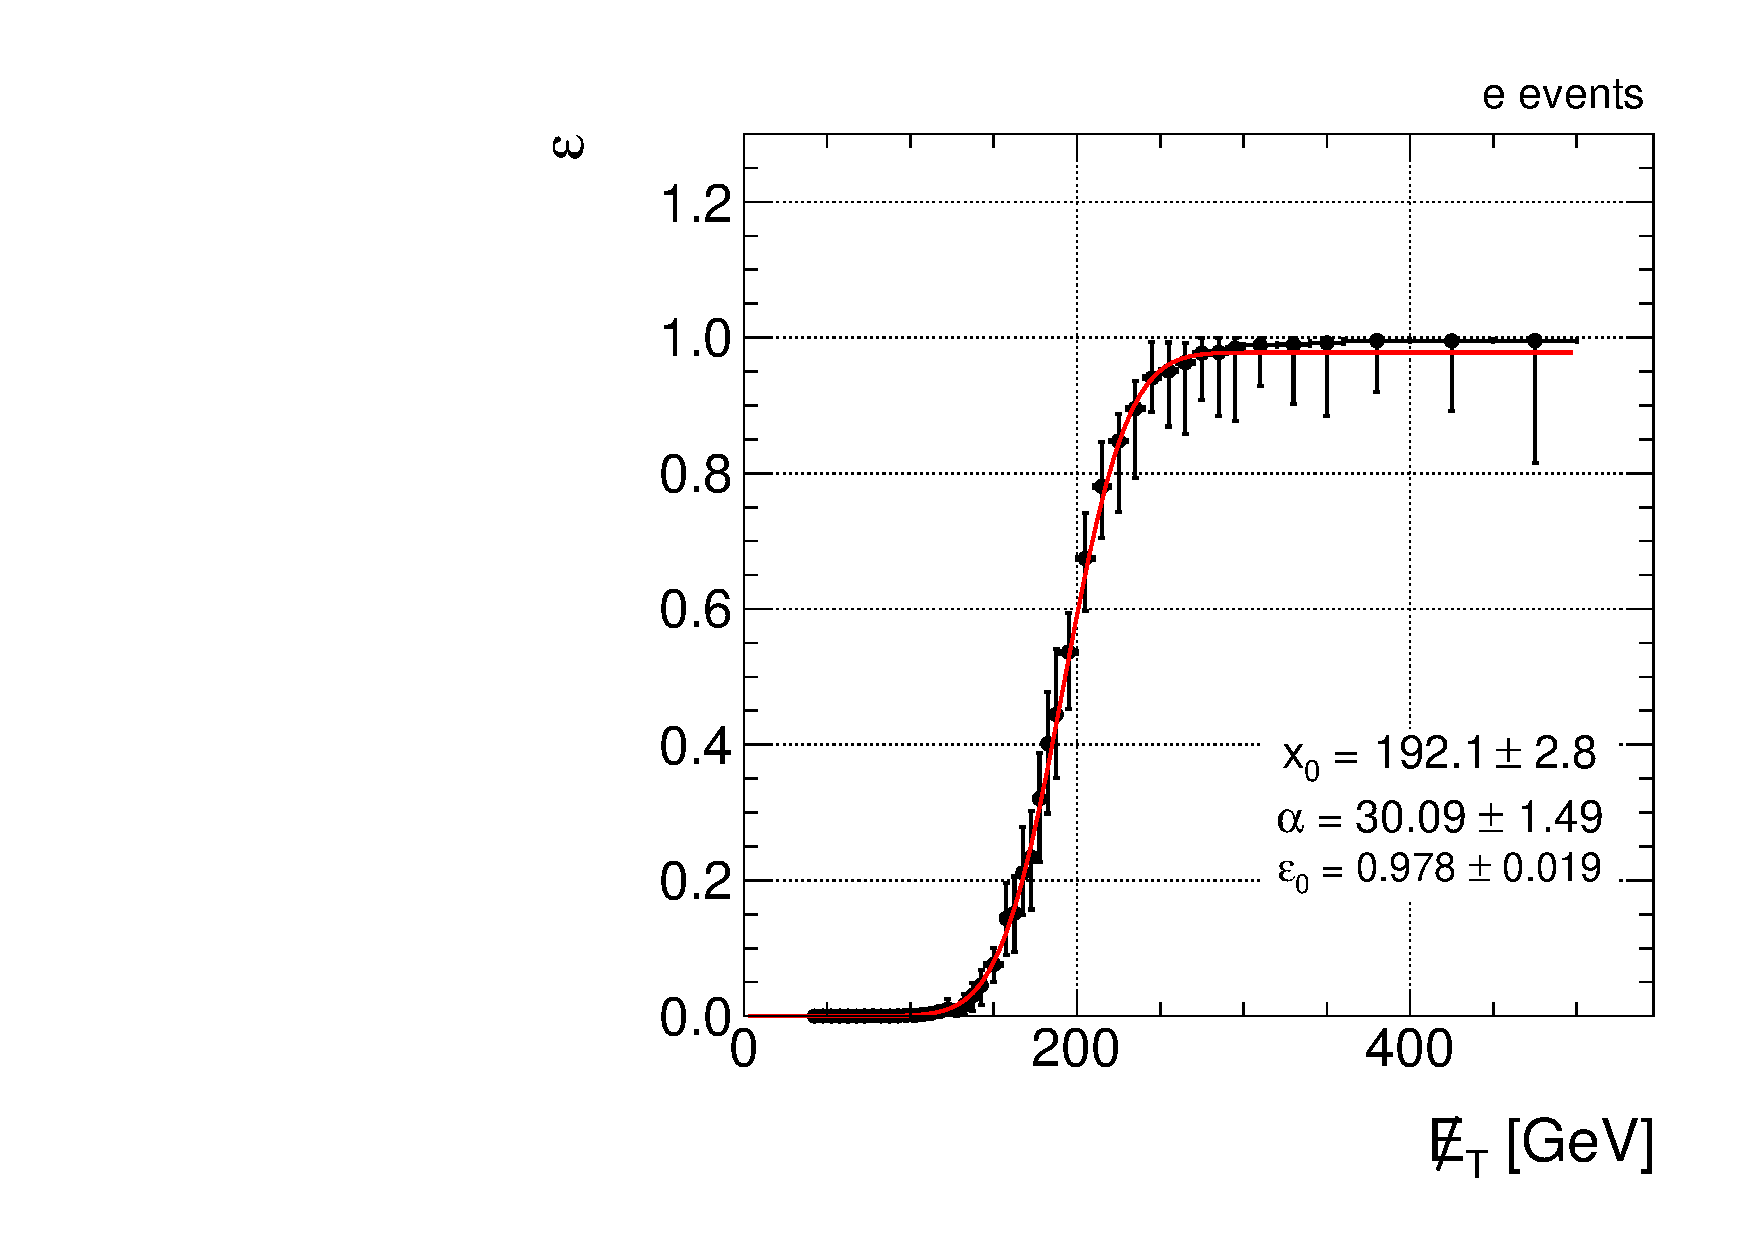
\includegraphics[width=0.48\textwidth]{figures/wjets-e-meteff.pdf}
  \caption{Efficiency turn-on curves of HLT\_PFMET170\_NoiseCleaned for $\ttbar+$DM EFT signal with $M_{\chi}=1$ (left), and for electron events in $\Wjets$ passing a single electron trigger (right). Events are required to have at least four jets.}
  \label{fig:meteff_1}
\end{figure}

The offline event selection requires,
\begin{itemize}
\item $\met > 250\:\GeV$, to be on the plateau of the efficiency turn-on curve,
\item at least $4$ AK4CHS jets with $\pt>30\:\GeV$ and $|\eta|<4$,
  \begin{itemize}
  \item at least $2$ of which have $|\eta|<2.4$ and $\Bot$-tagged,
  \end{itemize}
\item no muons passing ``Loose'' selection with $\pt>10\:\GeV$ and $|\eta|<2.4$,
\item no electrons passing ``Veto'' selection with $\pt>10\:\GeV$ and $|\eta|<2.5$,
\item $\min_{i=1,\ldots,6}\Delta\phi\left(j_i,\met\right)>1$, the minimum $\Delta\phi$ between jet and $\met$ considering up to the sixth leading jet.
\end{itemize}

The $\min_{i=1,\ldots,6}\Delta\phi\left(j_i,\met\right)$ distribution after all other selection cuts is shown in Fig.~\ref{fig:dphijetmet6}. The cut on this variable reduces the QCD multi-jets background to negligible levels. It also reduces the $\ttbar$ background, which is predominantly semileptonic.%, because events with high $\met$ have a boosted $\Top$ quark and therefore the neutrino and $\Bot$ jet will be close to each other. 
It was studied that considering $\Delta\phi$ for up to the sixth leading jet performs better than considering fewer number of jets and better than considering all jets. These studies are presented in Appendix~\ref{app:dphijetmet}.

\begin{figure}[htbp]
  \centering
  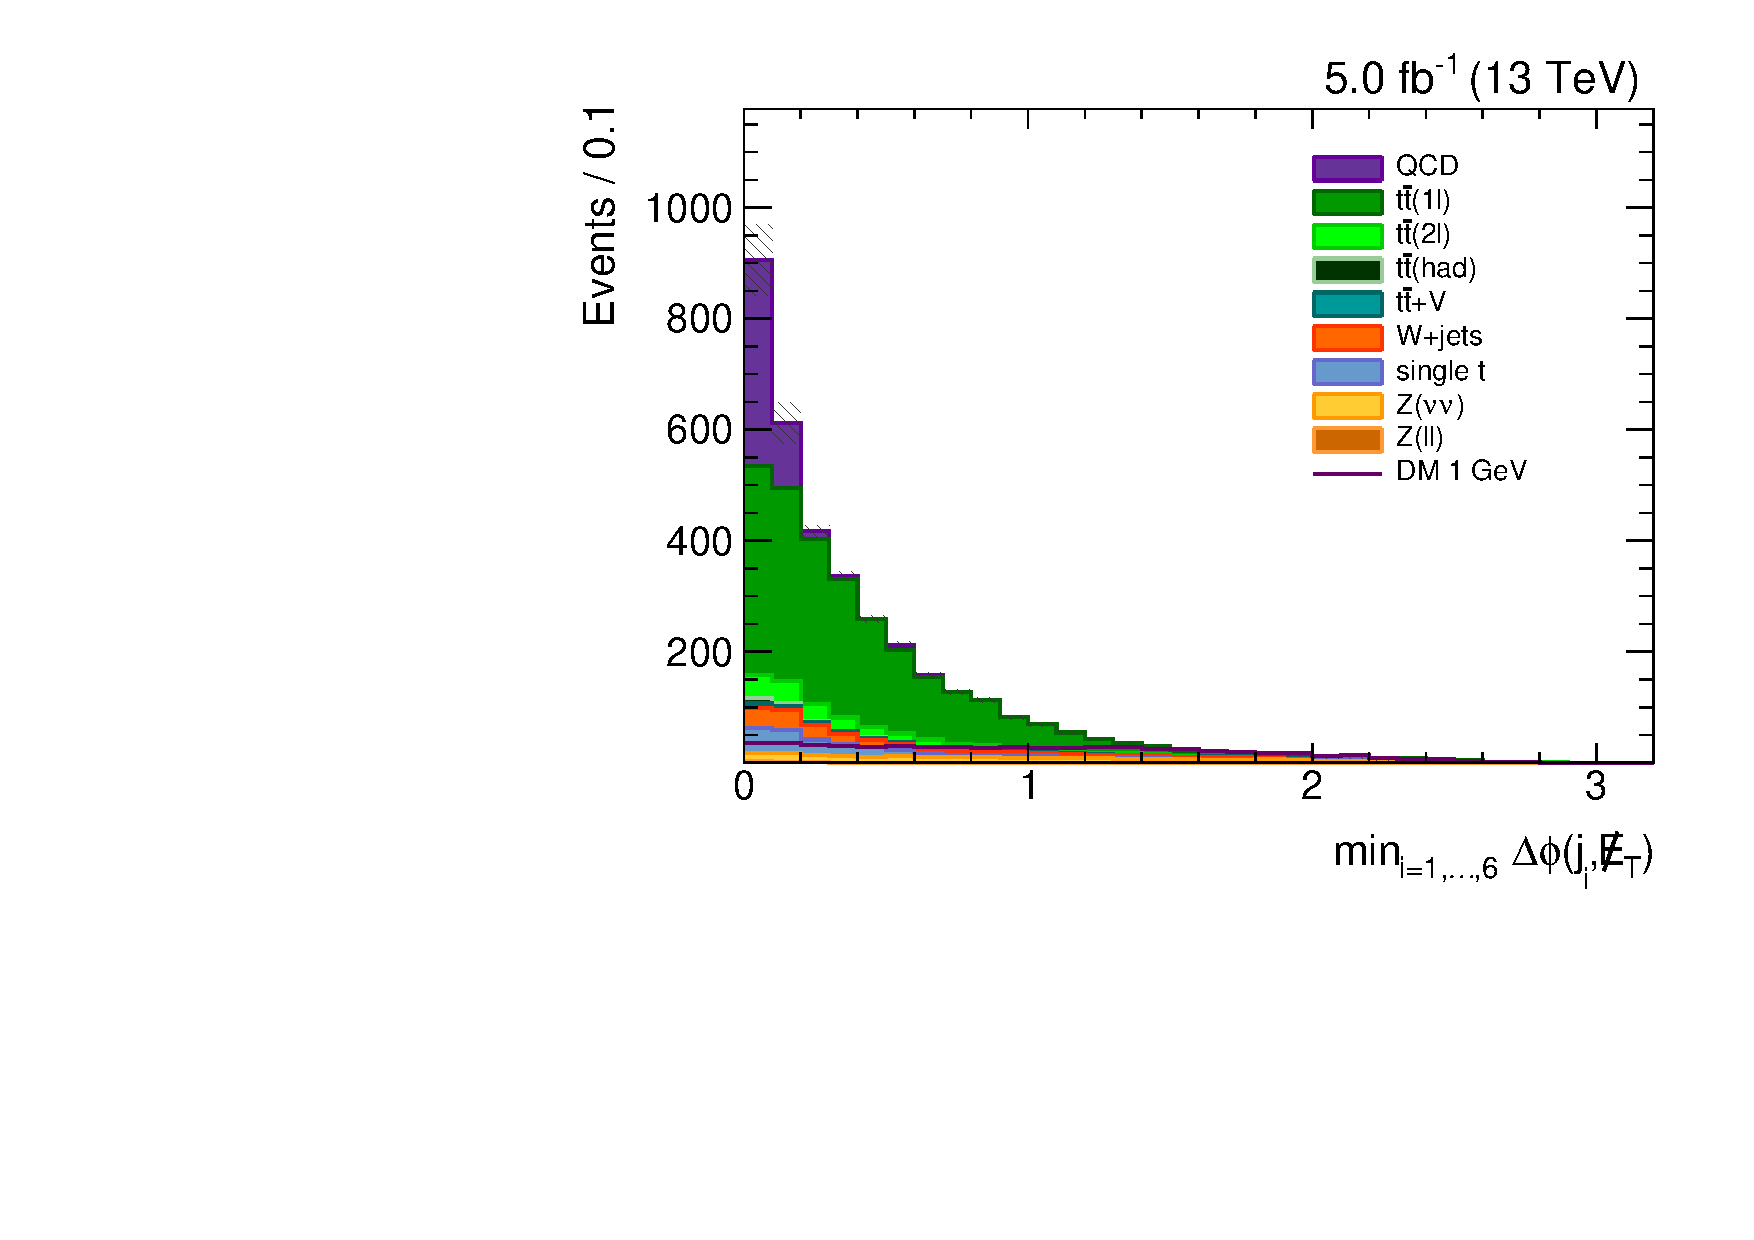
\includegraphics[width=0.48\textwidth]{figures/hadronic-incl-dphijetmet6.pdf}
  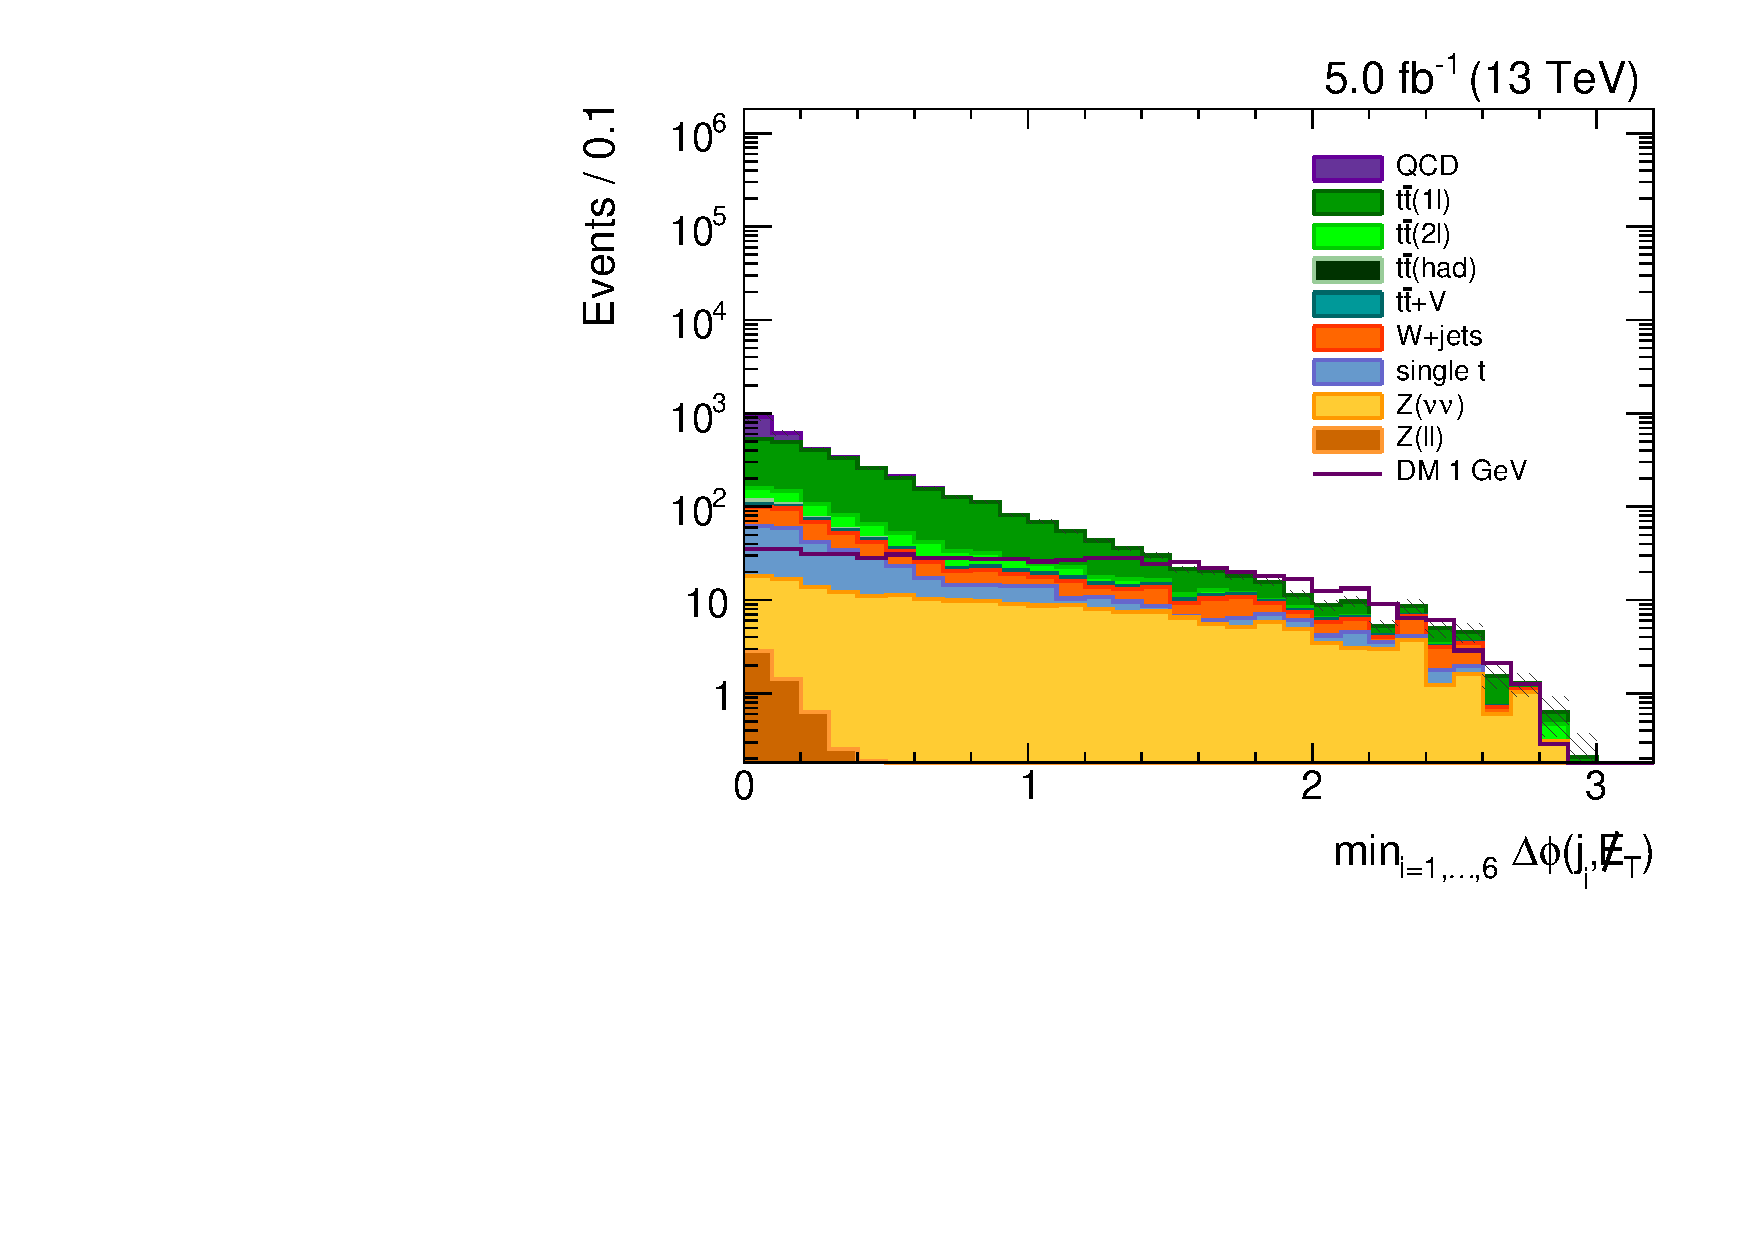
\includegraphics[width=0.48\textwidth]{figures/hadronic-incl-dphijetmet6log.pdf}
  \caption{The $\min_{i=1,\ldots,6}\Delta\phi\left(j_i,\met\right)$ distribution in linear scale (left) and log scale (right).}
  \label{fig:dphijetmet6}
\end{figure}

The $\met$ distributions before and after cutting on $\min_{i=1,\ldots,6}\Delta\phi\left(j_i,\met\right)$ are shown in Fig.~\ref{fig:incl_hadronic_met}. The expected yields for $5\:\ifb$ after selection are shown in Table~\ref{tab:incl_hadronic_yields}.

\begin{figure}[htbp]
  \centering
  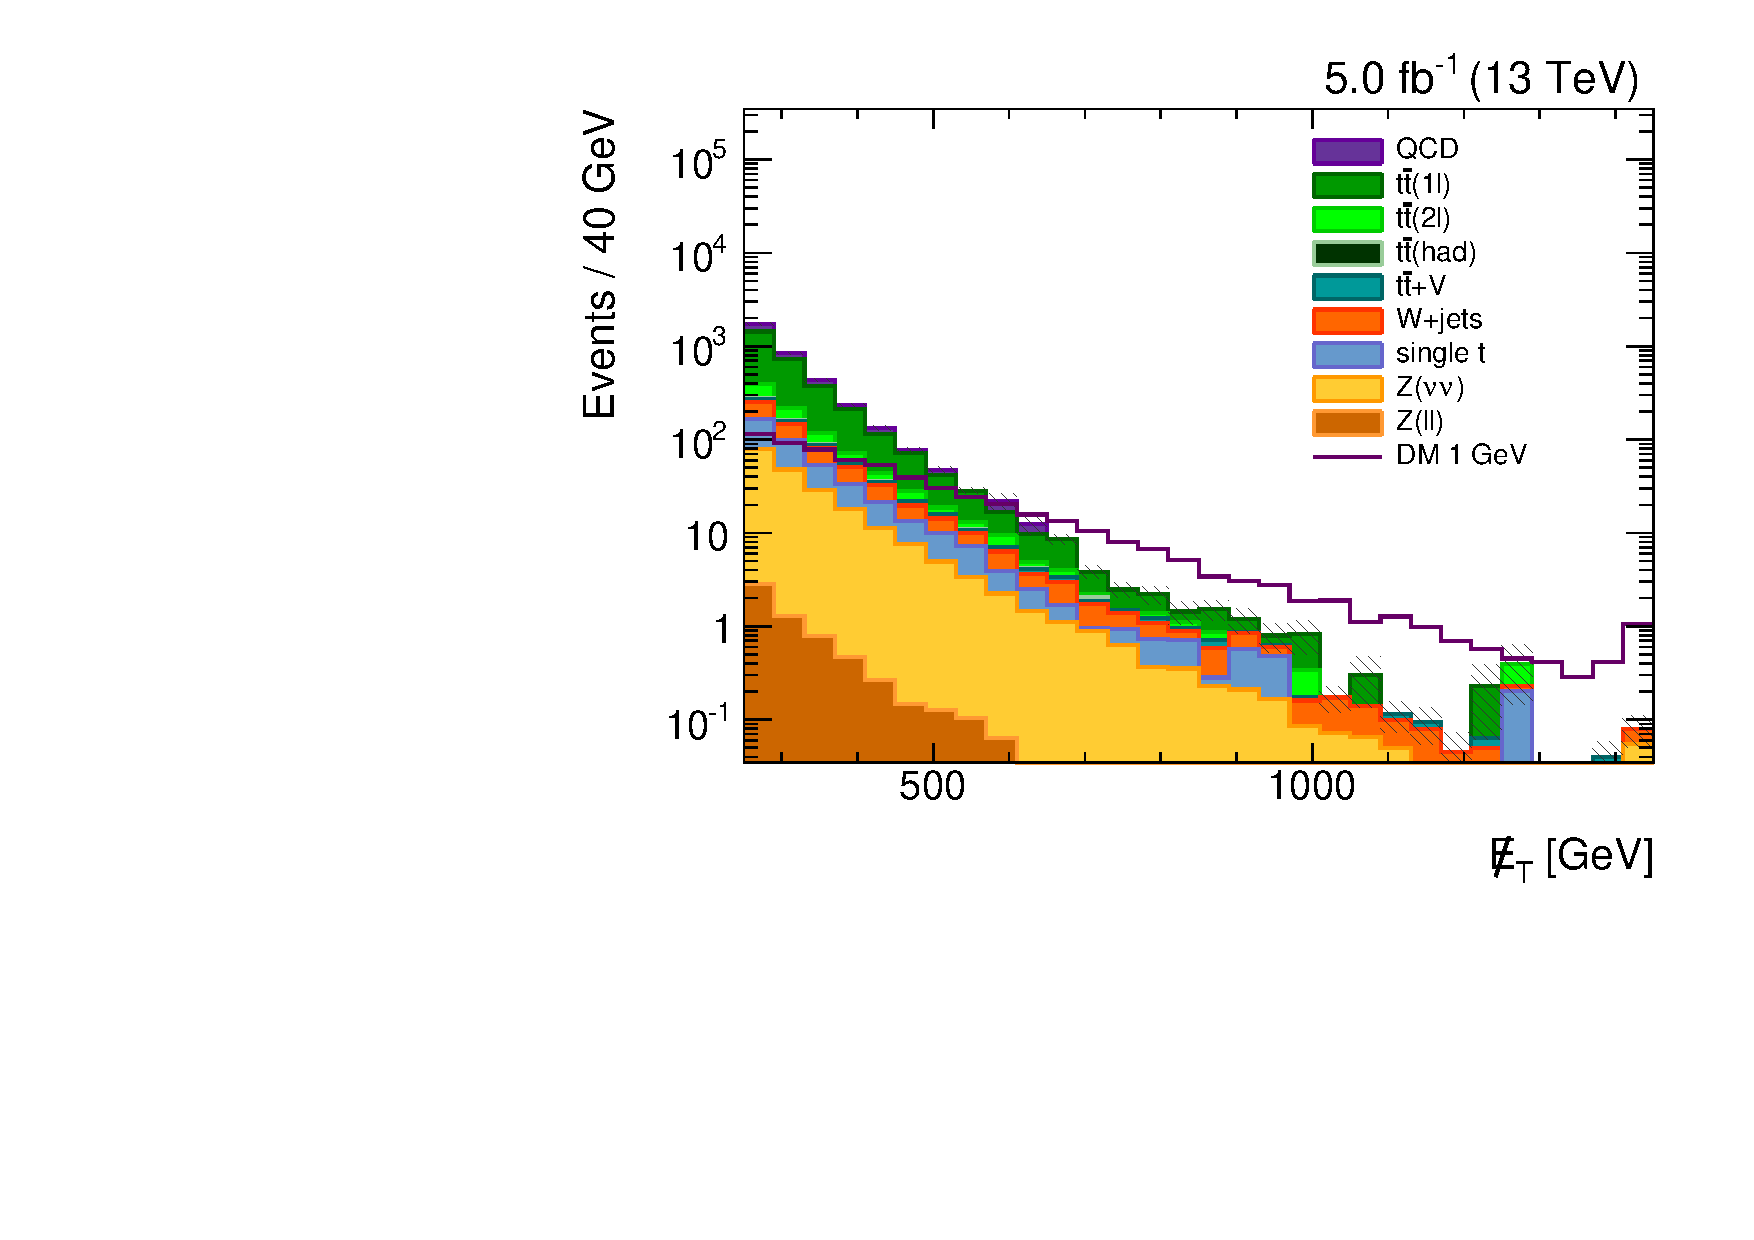
\includegraphics[width=0.48\textwidth]{figures/hadronic-incl-metlog_nodphi.pdf}
  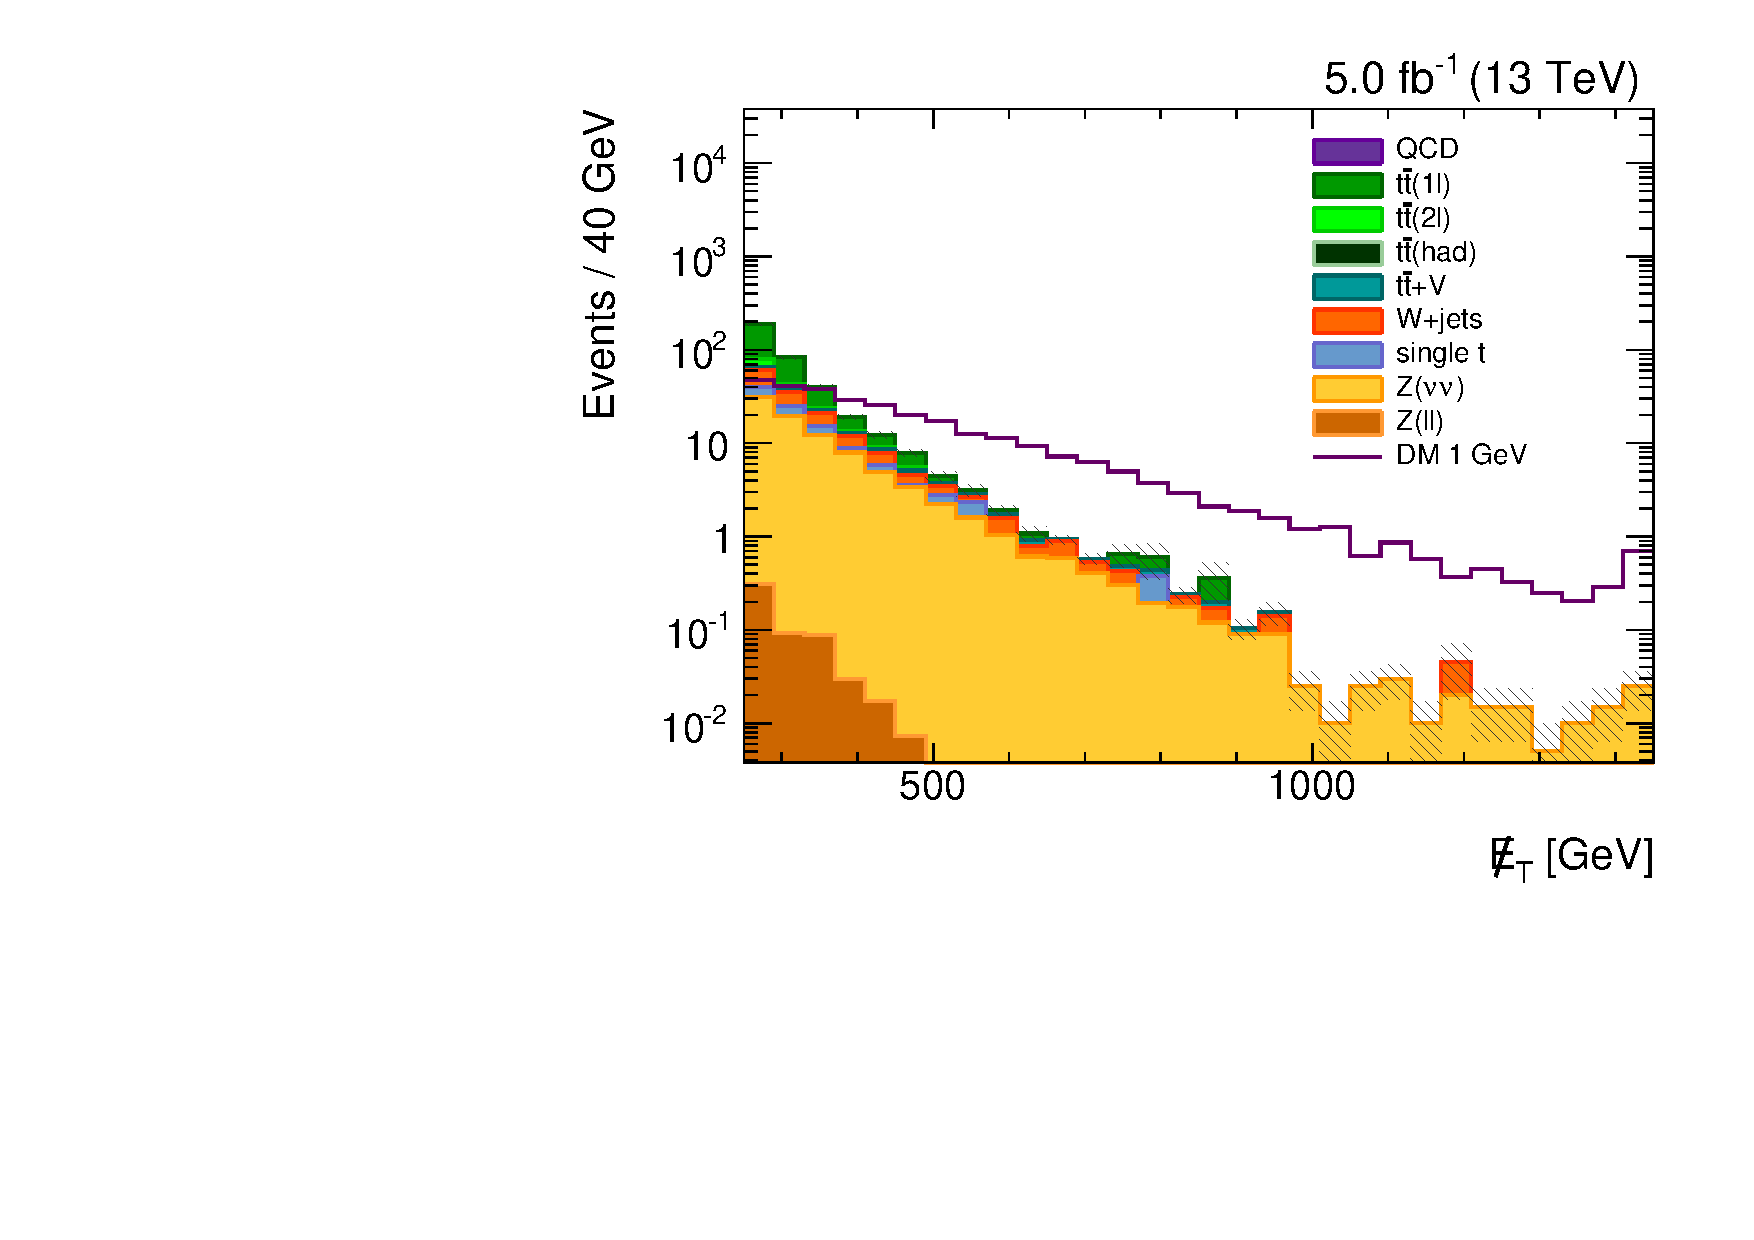
\includegraphics[width=0.48\textwidth]{figures/hadronic-incl-metlog.pdf}
  \caption{The $\met$ distribution before (left) and after (right) the cut on $\min_{i=1,\ldots,6}\Delta\phi\left(j_i,\met\right)$. Note that the right-most bin includes overflow.}
  \label{fig:incl_hadronic_met}
\end{figure}

\begin{table}[!ht]
\centering
\begin{tabular}{|c|r|}
\hline
  Process               & \multicolumn{1}{|c|}{Yields} \\
\hline
  \Z\To\Lep\Lep         & $  0.54 \pm 0.12$ \\
  \Z\To\Nu\Nu           & $ 86.09 \pm 1.82$ \\
  Single \Top           & $ 21.36 \pm 1.89$ \\
  \Wjets                & $ 45.42 \pm 3.11$ \\
  QCD                   & $  0.00 \pm 0.00$ \\
  $\ttbar+V$            & $ 11.19 \pm 0.40$ \\
  $\ttbar(\mbox{had})$  & $  0.00 \pm 0.00$ \\
  $\ttbar(1\Lep)$       & $179.61 \pm 5.42$ \\
  $\ttbar(2\Lep)$       & $ 21.74 \pm 1.88$ \\
\hline
  SM expected           & $365.94 \pm 7.04$ \\
\hline
  $M_\chi=1\:\GeV$      & $289.61 \pm 3.45$ \\
\hline
\end{tabular}
\caption{Expected yields for $5\:\ifb$ after the inclusive selection for the hadronic channel.}
\label{tab:incl_hadronic_yields}
\end{table}

\subsection{Inclusive Selection: Semileptonic channel}
\label{subsec:sel_incl_semilept}

Events for the semileptonic channel are obtained with HLT\_Ele27\_eta2p1\_WP75\_Gsf in MC and HLT\_Ele27\_eta2p1\_WPLoose\_Gsf in data, a single electron trigger, and HLT\_IsoMu27, a single muon trigger. Kinematic thresholds on the trigger objects constrain the offline requirements on the electron or muon to $\pt>30\:\GeV$ and $|\eta|<2.1$ in order to avoid the sharp efficiency turn-on. Trigger efficiencies measured with the tag-and-probe method are shown in Fig.~\ref{fig:seleff} and Fig.~\ref{fig:smueff} for the single electron HLT\_Ele27\_eta2p1\_WP75\_Gsf trigger measured in MC and HLT\_Ele27\_eta2p1\_WPLoose\_Gsf in data and HLT\_IsoMu27 in data and MC, respectively.

The data-to-MC trigger efficiency scale factors for the single electron HLT\_Ele27\_eta2p1\_WP75\_Gsf trigger and the single muon HLT\_IsoMu27 trigger have been computed in $\pt$-$|\eta|$ bins using standard tag-and-probe procedures and are shown in Table~\ref{tab:sf_ele} and Table~\ref{tab:sf_mu} respectively. 

\begin{table}[!ht]
\centering
\begin{tabular}{|c|c|c|c|c|}
\hline
&                                &                                &                                &                                                                 \\   
& $0.0 < |\eta| < 0.4$ & $0.4 < |\eta| < 1.4$ & $1.4 < |\eta| < 1.6$ & $1.6 < |\eta| < 2.1$    \\
&                                &                                &                                &                                                                \\   
\hline
$30 < \pt <  32$ &  $0.936 \pm  0.006$  &  $0.947 \pm  0.006$  &  $0.794 \pm  0.026$  &  $0.893 \pm  0.008$ \\
\hline
$32 < \pt <  35$ &  $0.958 \pm  0.003$  &  $0.980 \pm  0.003$  &  $0.914 \pm  0.013$  &  $0.954 \pm  0.005$ \\
\hline
$35 <\pt  <  40$ &  $0.970 \pm  0.002$  &  $0.998 \pm  0.001$  &  $0.999 \pm  0.006$  &  $0.958 \pm  0.003$ \\
\hline
$40 < \pt <  50$ &  $0.980 \pm  0.001$  &  $1.005 \pm  0.001$  &  $0.998 \pm  0.004$  &  $0.958 \pm  0.002$ \\
\hline
$50 < \pt < 200$ & $0.998 \pm  0.001$  &  $1.012 \pm  0.001$  &  $1.004 \pm  0.005$  &  $0.944 \pm  0.003$ \\
\hline
      $\pt > 200$   & $1.011 \pm  0.031$  &  $1.012 \pm  0.019$  &  $0.947 \pm  0.115$  &  $0.950 \pm  0.077 $\\	
\hline	
	
\end{tabular}
\caption{Data-to-MC efficiency scale factors for single electron trigger by $\pt$-$|\eta|$ bins}
\label{tab:sf_ele}
\end{table}


\begin{table}[!ht]
\centering
\begin{tabular}{|c|c|c|c|c|c|c|}
\hline
  &                                &                                &                                &                                 &                                &                             \\   
  & $0.0 < |\eta| < 0.4$ & $0.4 < |\eta| < 0.8$ & $0.8 < |\eta| < 1.2$ & $1.2 < |\eta| < 1.6$ & $1.6 < |\eta| < 2.1$ & $2.1 < |\eta| < 2.4$ \\
  &                                &                                &                                &                                 &                                &                             \\   

\hline
	$30 < \pt <   32$ &  $0.963 \pm  0.004$  & $ 1.004 \pm  0.003 $ &  $0.982 \pm  0.005 $ &  $0.972 \pm  0.004$  &  $0.937 \pm  0.005 $ &  $0.910 \pm  0.010$ \\
\hline	
  	$32 < \pt <   34$ &  $0.972 \pm  0.003$  & $ 1.008 \pm  0.003$  &  $0.995 \pm  0.004 $ &  $0.987 \pm  0.004 $ & $ 0.948 \pm  0.005$  & $ 0.917 \pm  0.009$ \\
\hline  	
	$34 < \pt <   36 $&  $0.979 \pm  0.003$  &  $1.003 \pm  0.002$  &  $0.988 \pm  0.004 $ &  $0.990 \pm  0.003$  &  $0.945 \pm  0.004 $ & $ 0.921 \pm  0.008 $\\
\hline  	
	$36 < \pt <   38$ &  $0.977 \pm  0.002$  &  $1.001 \pm  0.002$  &  $0.980 \pm  0.003 $ &  $0.989 \pm  0.003$  & $ 0.951 \pm  0.004 $ & $ 0.923 \pm  0.007$ \\
\hline  	
	$38 < \pt <   40$ &  $0.977 \pm  0.002$  &  $0.999 \pm  0.002$  &  $0.984 \pm  0.003$  &  $0.988 \pm  0.002$  & $ 0.955 \pm  0.003$  & $ 0.928 \pm  0.007$ \\
\hline  	
	$40 < \pt <   45$ &  $0.977 \pm  0.001$  &  $0.996 \pm  0.001$  &  $0.978 \pm  0.002$  &  $0.990 \pm  0.001$  &  $0.955 \pm  0.002 $ &  $0.934 \pm  0.004 $\\
\hline  	
	$45 < \pt <   50$ &  $0.978 \pm  0.001$  & $ 0.996 \pm  0.001$  &  $0.979 \pm  0.002$  &  $0.993 \pm  0.001$  &  $0.956 \pm  0.002 $ & $ 0.939 \pm  0.004$ \\
\hline  	

	$50 < \pt <  200$ &  $0.977 \pm  0.002$  &  $0.994 \pm  0.001$  &  $0.976 \pm  0.002$  &  $0.994 \pm  0.001$  &  $0.958 \pm  0.002$  &  $0.955 \pm  0.004$ \\

\hline      	
	 $\pt >  200$ &  $0.993 \pm  0.031$  &  $0.998 \pm  0.027$  &  $1.005 \pm  0.047$  &  $0.982 \pm  0.038$  &  $0.959 \pm  0.062 $ &  $0.822 \pm  0.114 $\\
\hline
\end{tabular}
\caption{Data-to-MC efficiency scale factors for single muon HLT\_IsoMu27 by $\pt$-$|\eta|$ bins}
\label{tab:sf_mu}
\end{table}


\begin{figure}[htbp]
  \centering
  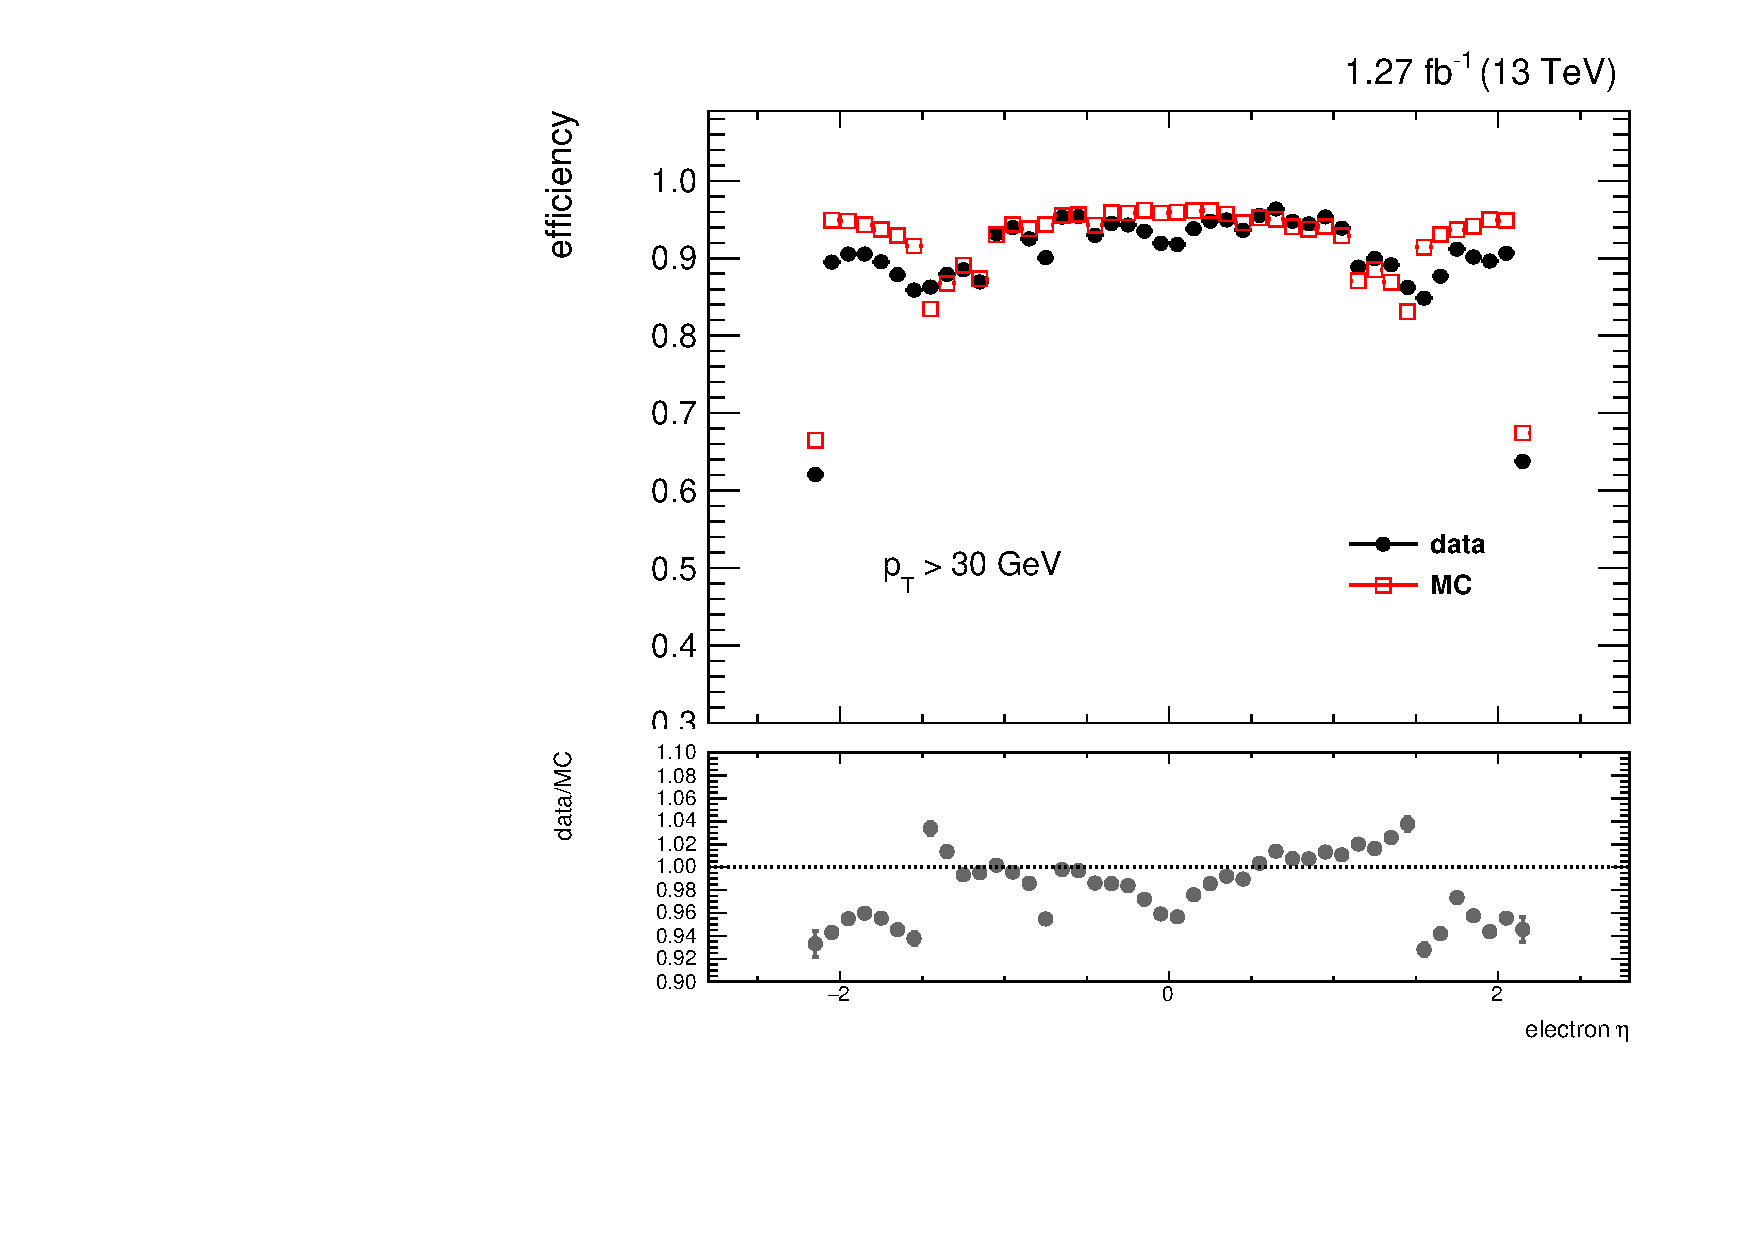
\includegraphics[width=0.48\textwidth]{figures/sel_effeta_dataMC.pdf}
  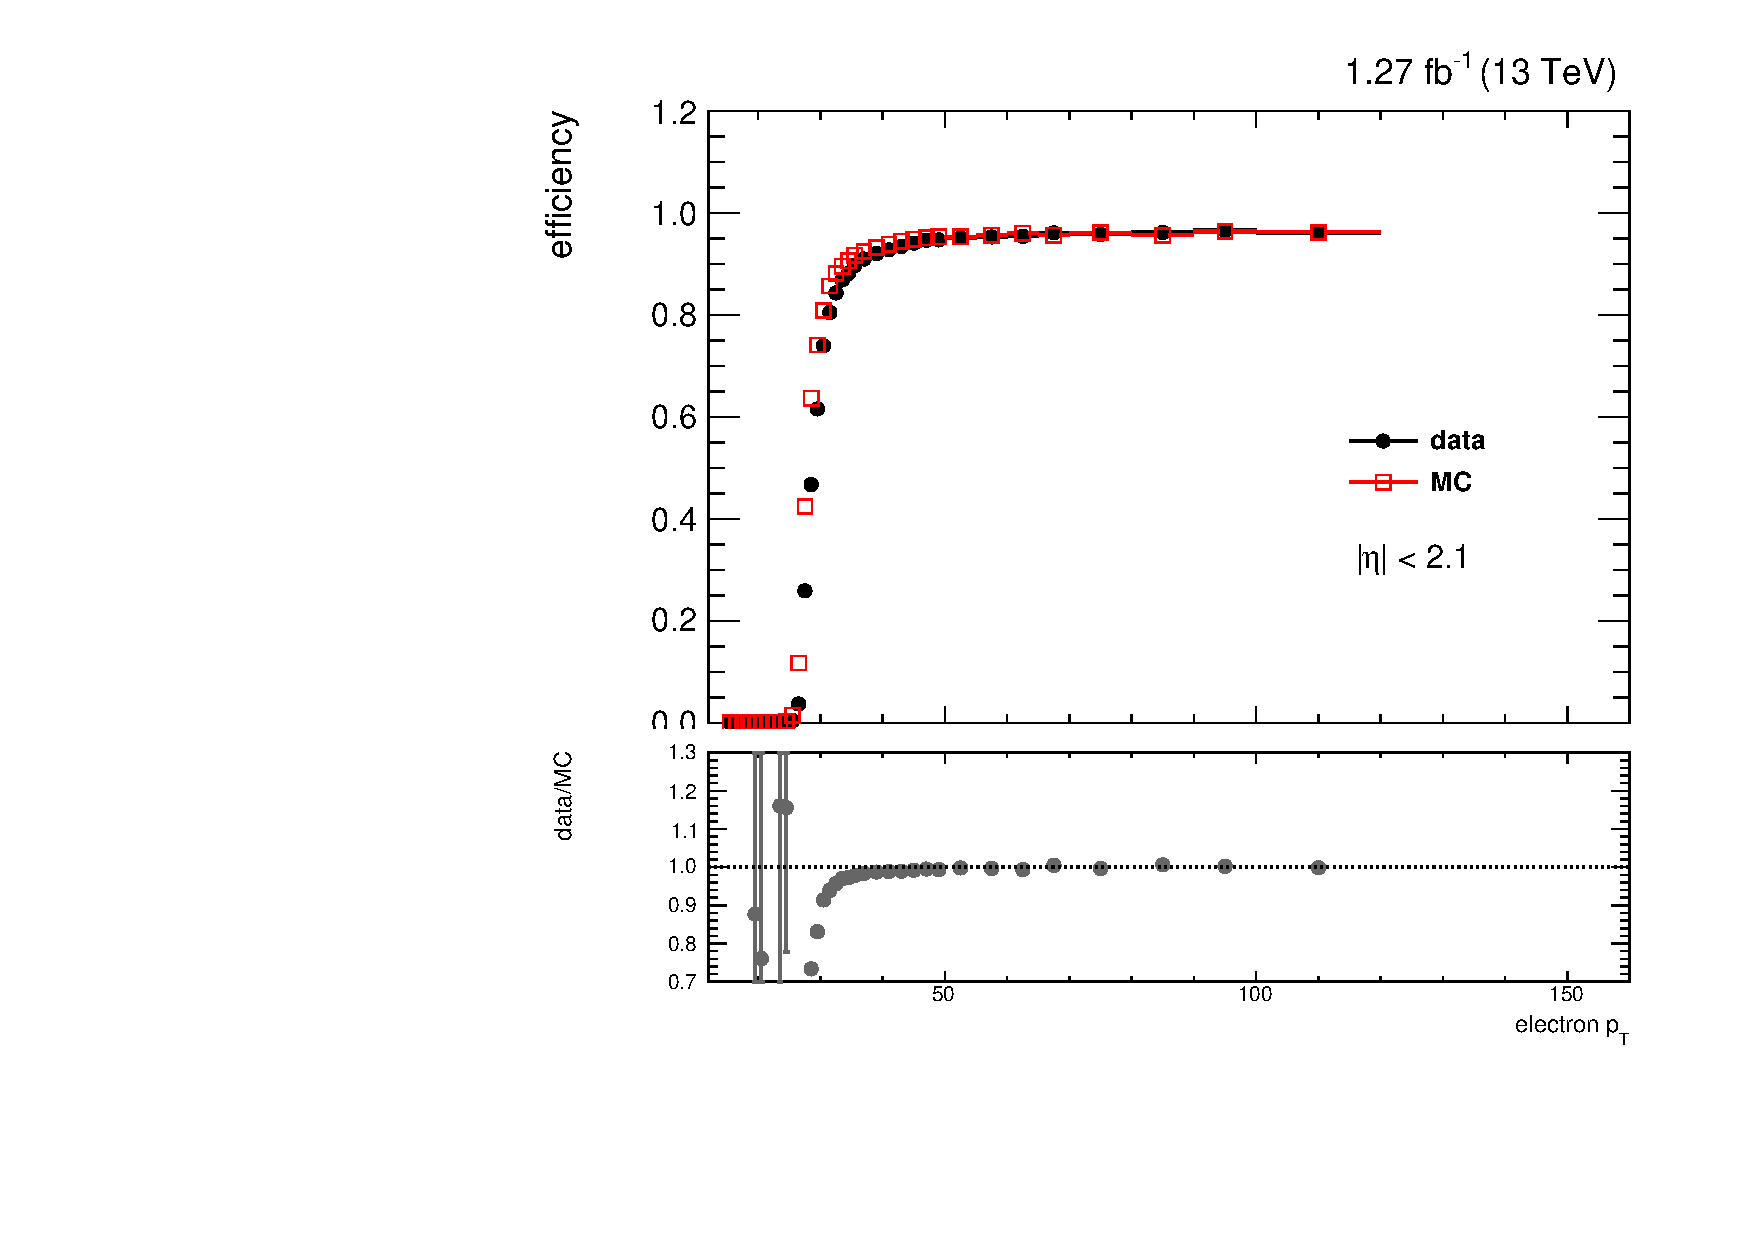
\includegraphics[width=0.48\textwidth]{figures/sel_effpt_dataMC.pdf}
  \caption{Efficiency of HLT\_Ele27\_eta2p1\_WP75\_Gsf in MC and HLT\_Ele27\_eta2p1\_WPLoose\_Gsf in data with respect to $\eta$ (left) and $\pt$ for $|\eta|<2.1$ (right).}
  \label{fig:seleff}
\end{figure}

\begin{figure}[htbp]
  \centering
  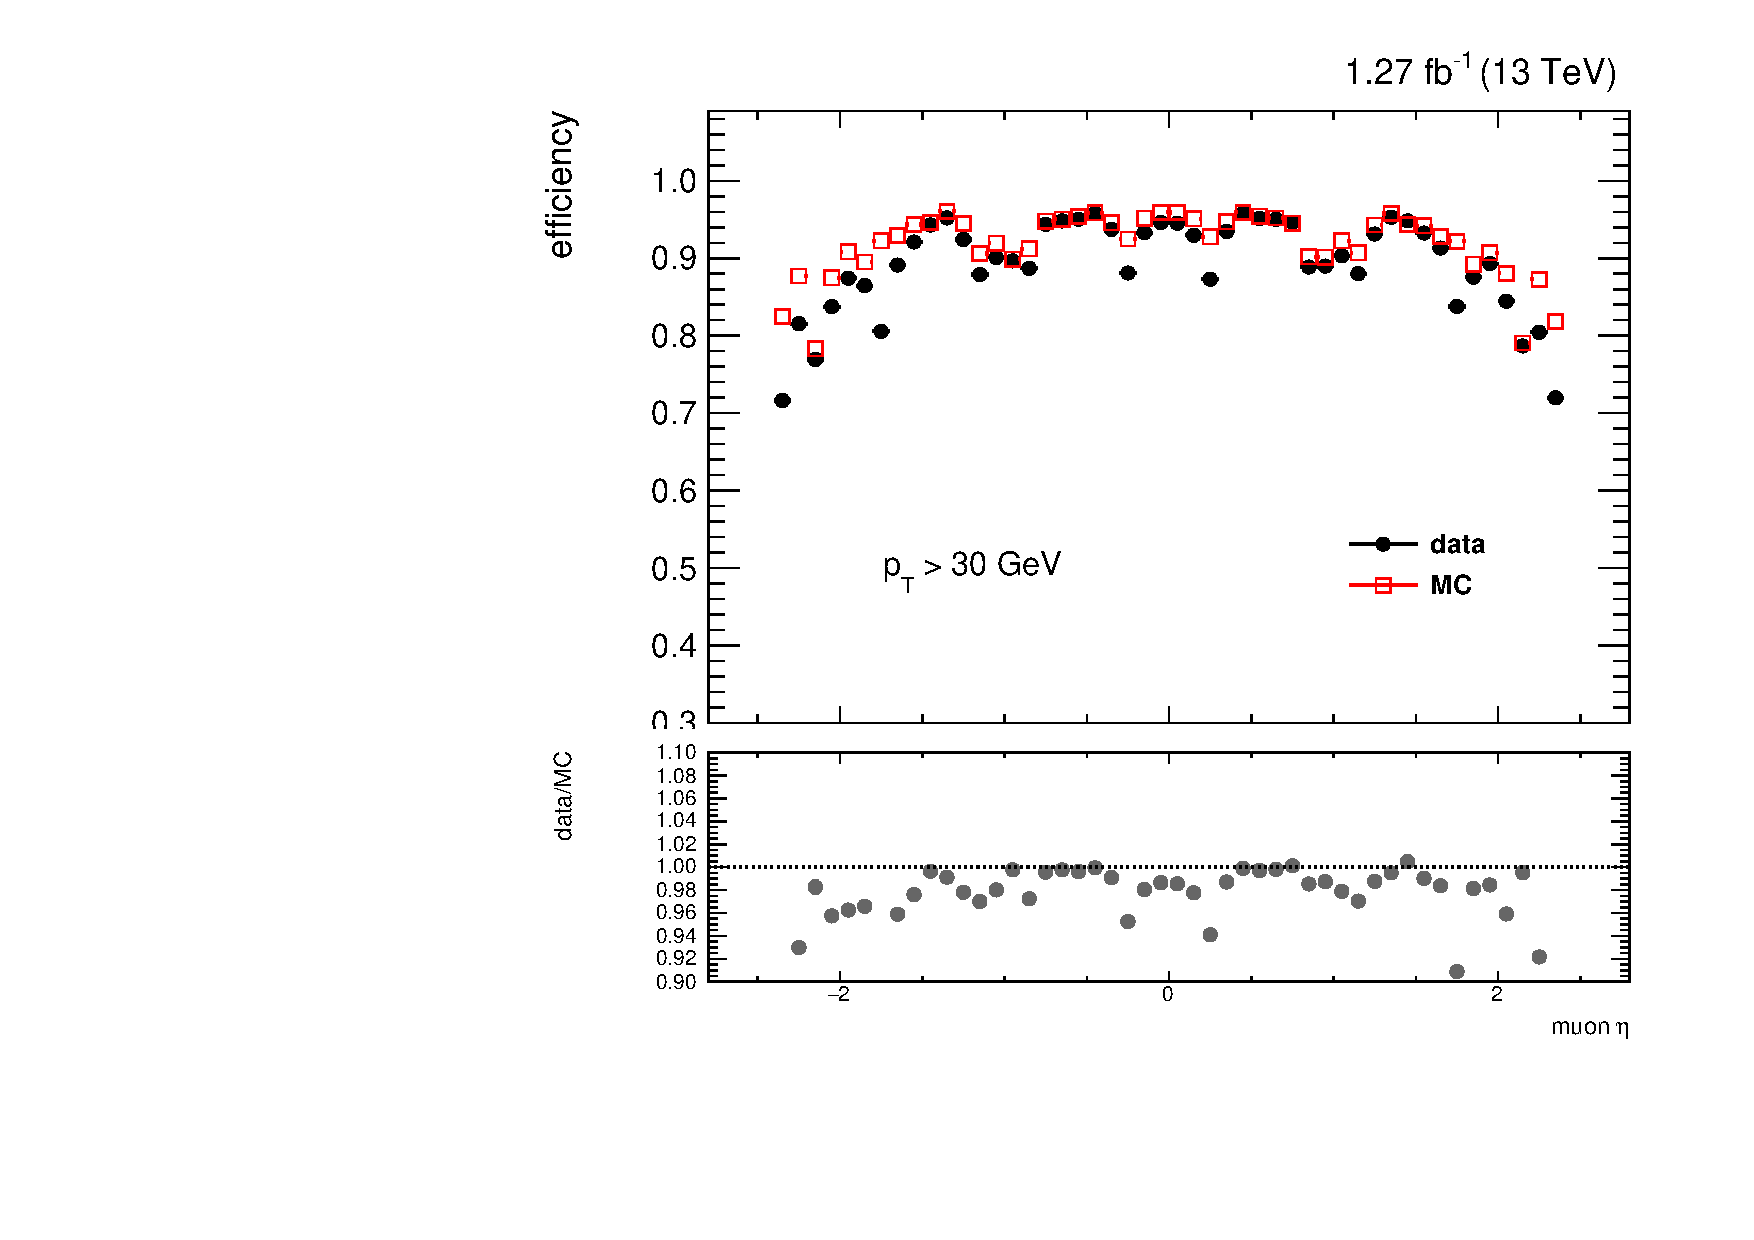
\includegraphics[width=0.48\textwidth]{figures/smu_effeta_dataMC.pdf}
  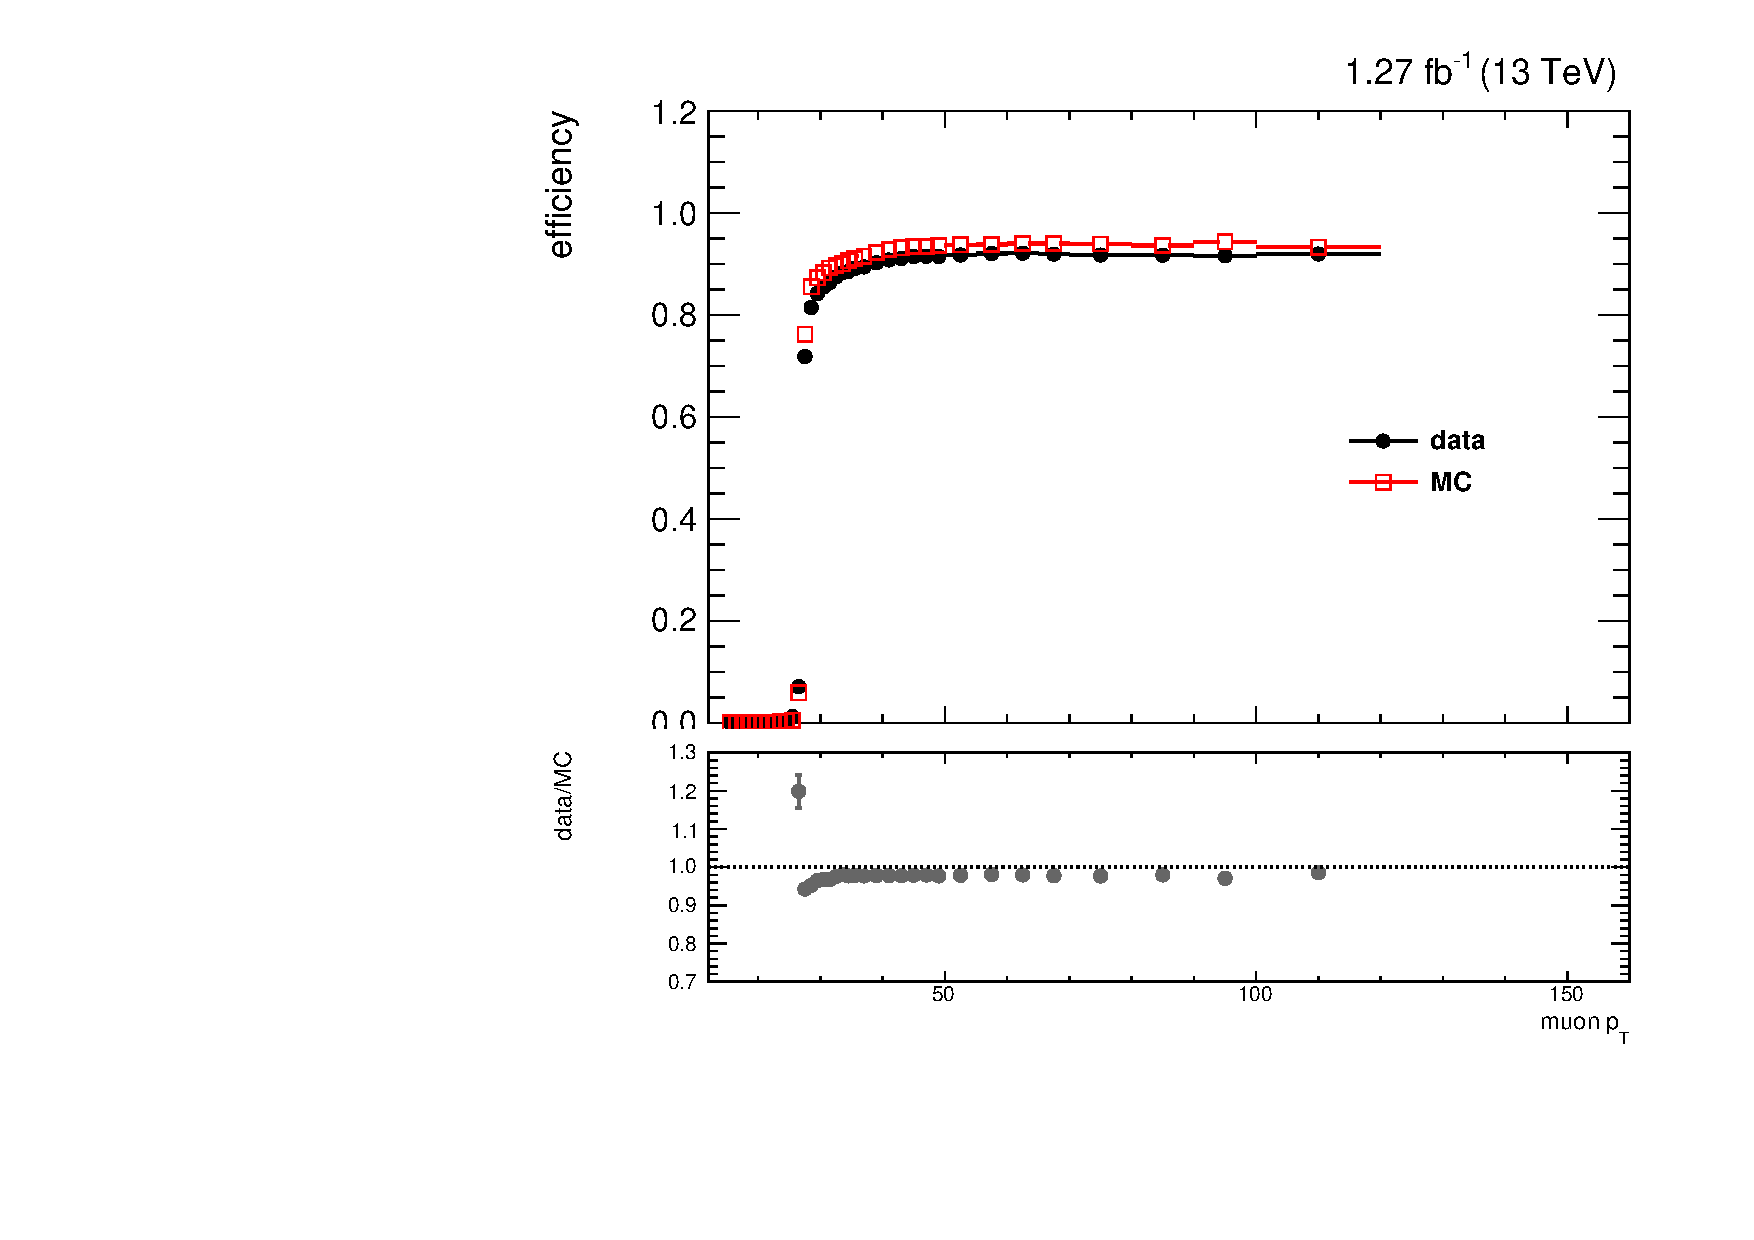
\includegraphics[width=0.48\textwidth]{figures/smu_effpt_dataMC.pdf}
  \caption{Efficiency of HLT\_IsoMu27 in data and MC with respect to $\eta$ (left) and $\pt$ for $|\eta|<2.4$ (right).}
  \label{fig:smueff}
\end{figure}

\clearpage

In order to greatly reduce semileptonic $\ttbar$ and $\Wjets$ background, events are required to have high transverse mass, $M_T$, defined as,
\begin{equation}
M_T = \sqrt{2\,\pt^{\Lep}\,\met \left(1-\cos\Delta\phi_{\Lep,\met}\right)}.
\end{equation}

The remaining $\ttbar$ background is predominantly from the dilepton channel. Two variables that help reject this background are $M_{T2}^W$ and $\min_{i=1,2}\Delta\phi\left(j_i,\met\right)$, the minimum $\Delta\phi$ between jet and $\met$ among the two leading jets. The offline event selection is,
\begin{itemize}
\item $\met > 160\:\GeV$,
\item exactly one electron or muon passing ``Tight'' selection with $\pt>30\:\GeV$ and $|\eta|<2.1$ and matched to the trigger object,
\item at least $3$ AK4CHS jets with $\pt>30\:\GeV$ and $|\eta|<4$,
  \begin{itemize}
  \item at least one of which has $|\eta|<2.4$ and $\Bot$-tagged,
  \end{itemize}
\item no additional muons passing ``Loose'' selection with $\pt>10\:\GeV$ and $|\eta|<2.4$,
\item no additional electrons passing ``Veto'' selection with $\pt>10\:\GeV$ and $|\eta|<2.5$,
\item $M_T > 160\:\GeV$,
\item $M_{T2}^W > 200\:\GeV$,
\item $\min_{i=1,2}\Delta\phi\left(j_i,\met\right)>1.2$.
\end{itemize}

\begin{figure}[htbp]
  \centering
  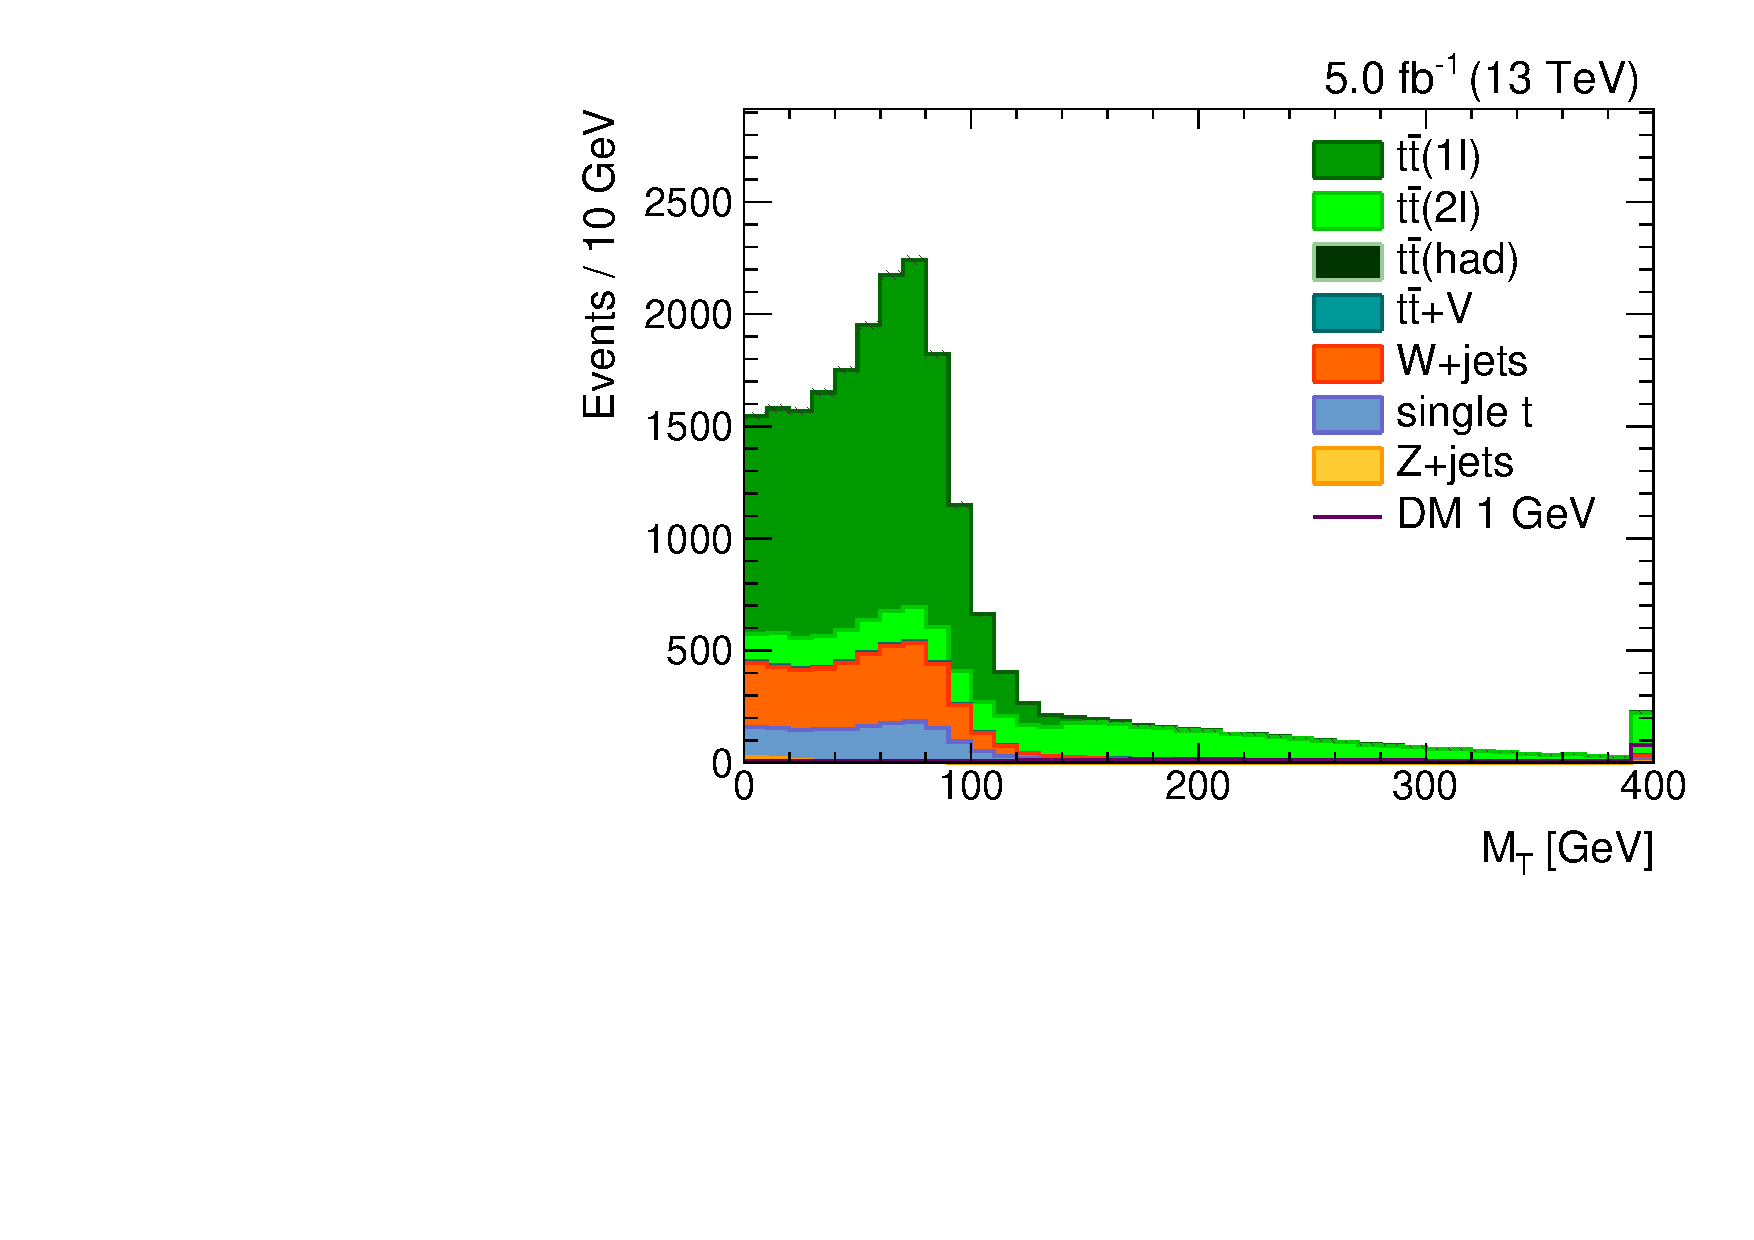
\includegraphics[width=0.48\textwidth]{figures/semilept-incl-mt_l.pdf}
  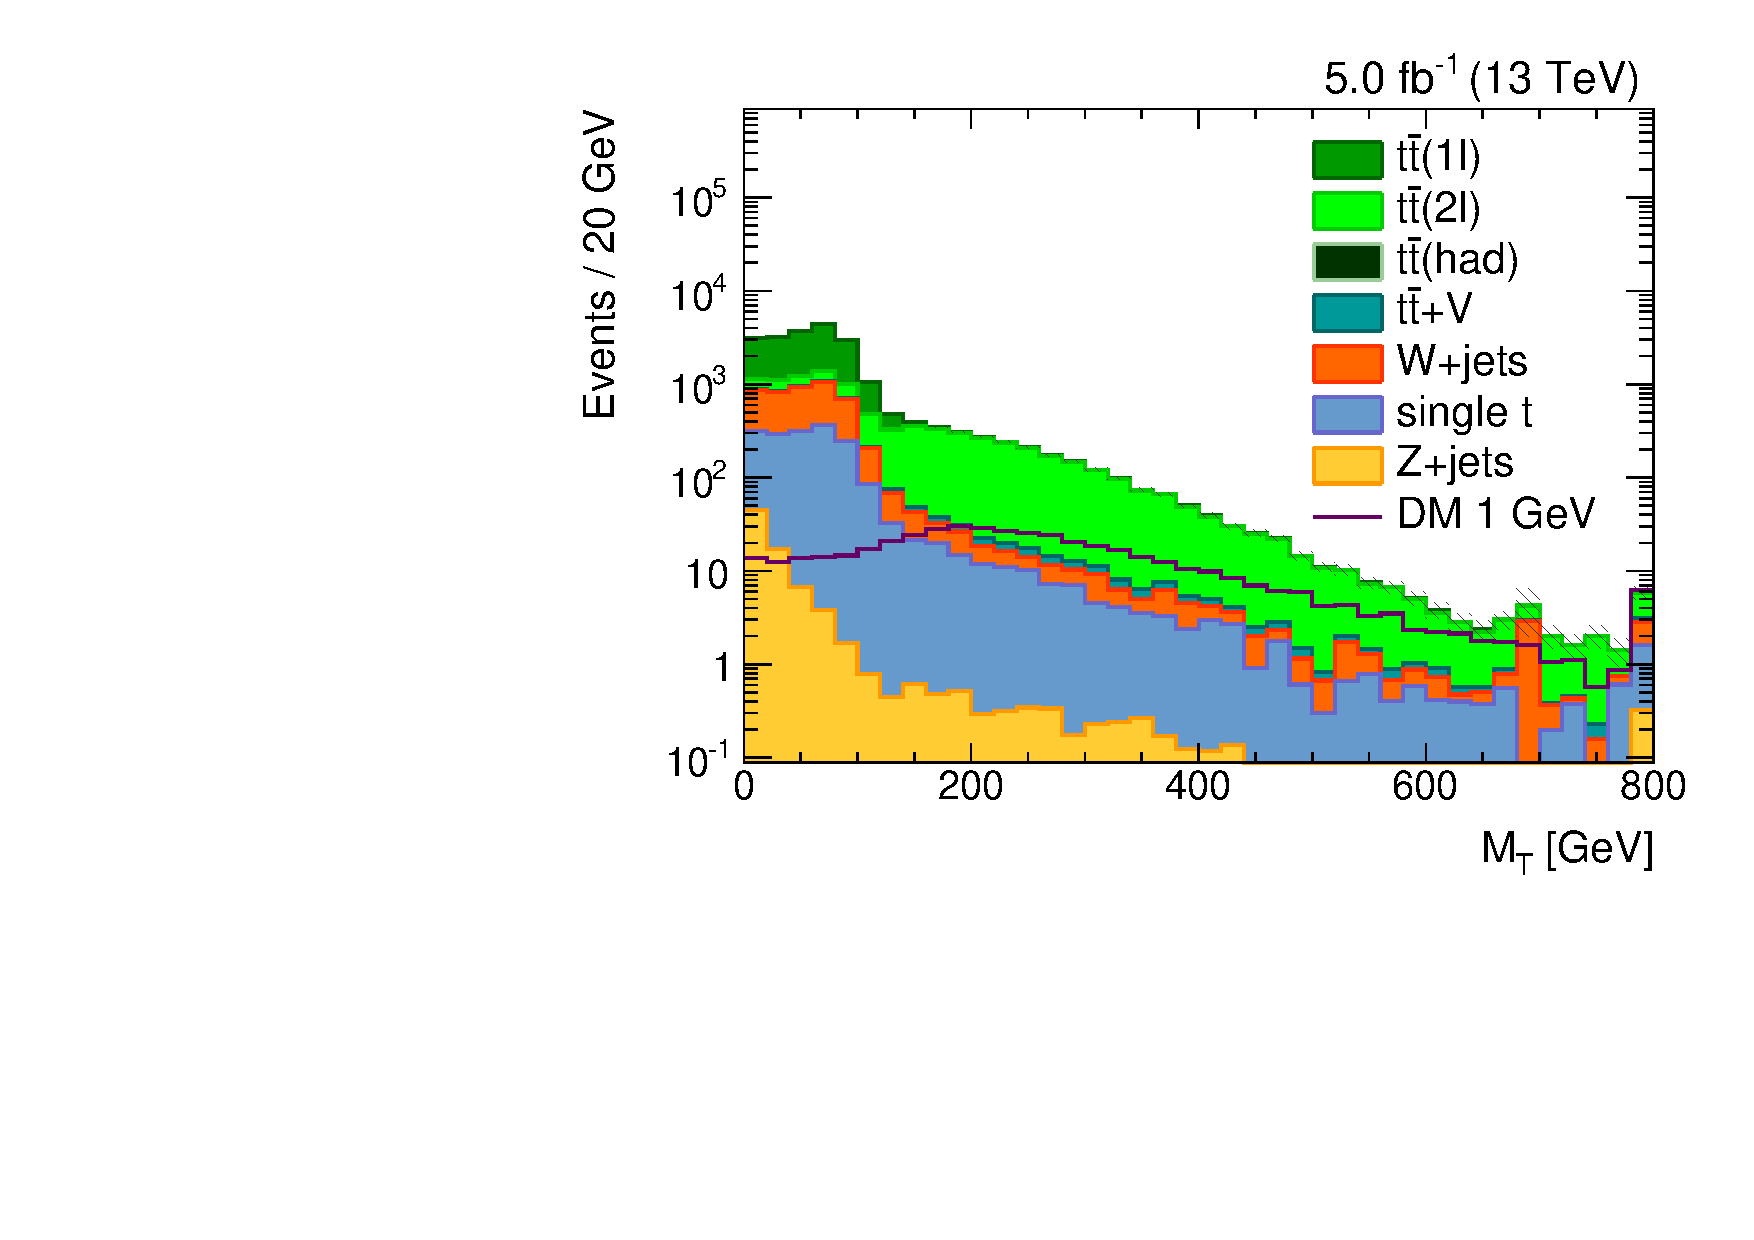
\includegraphics[width=0.48\textwidth]{figures/semilept-incl-mtlog_l.pdf}
  \caption{The $M_T$ distribution in linear (left) and log (right) scales. Note that the right-most bin includes overflow.}
  \label{fig:incl_semilept_mt}
\end{figure}

\begin{figure}[htbp]
  \centering
  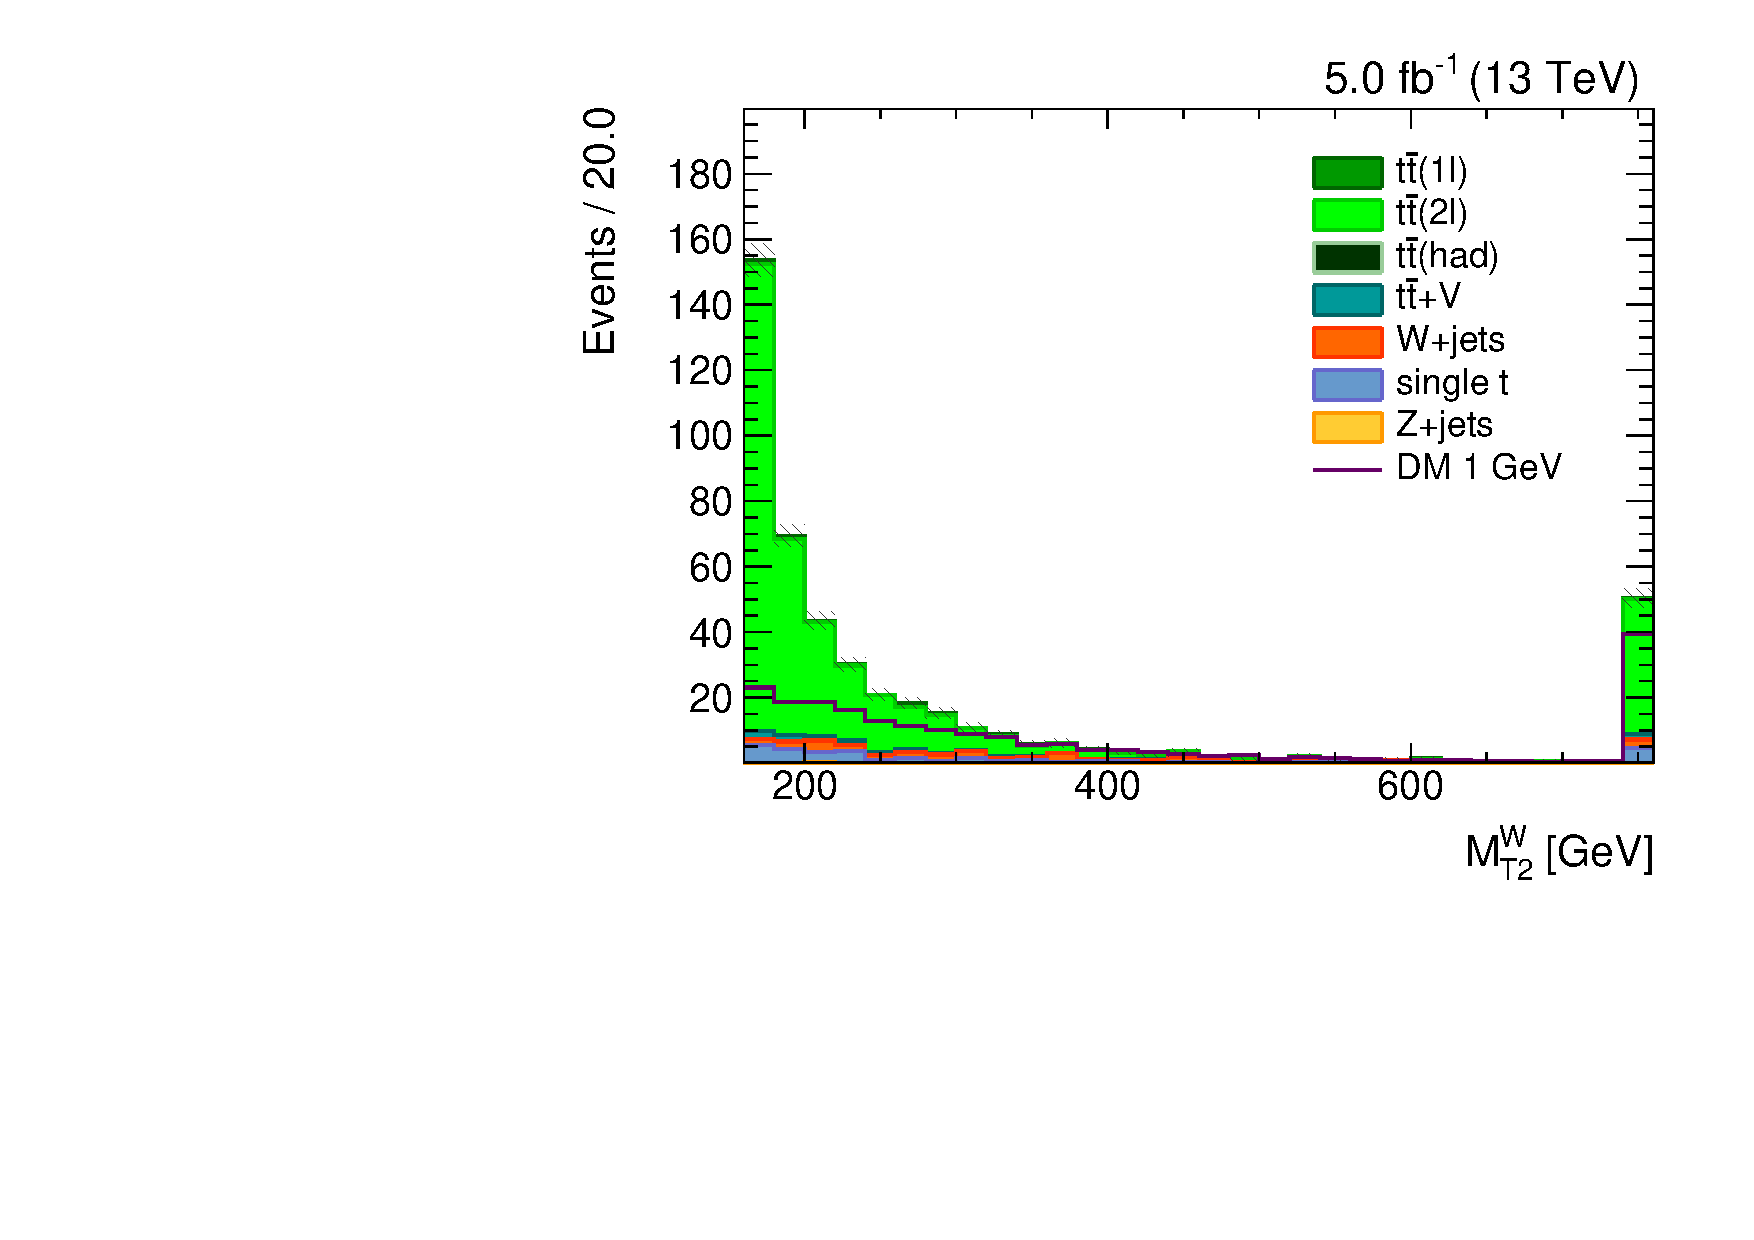
\includegraphics[width=0.48\textwidth]{figures/semilept-incl-mt2w_l.pdf}
  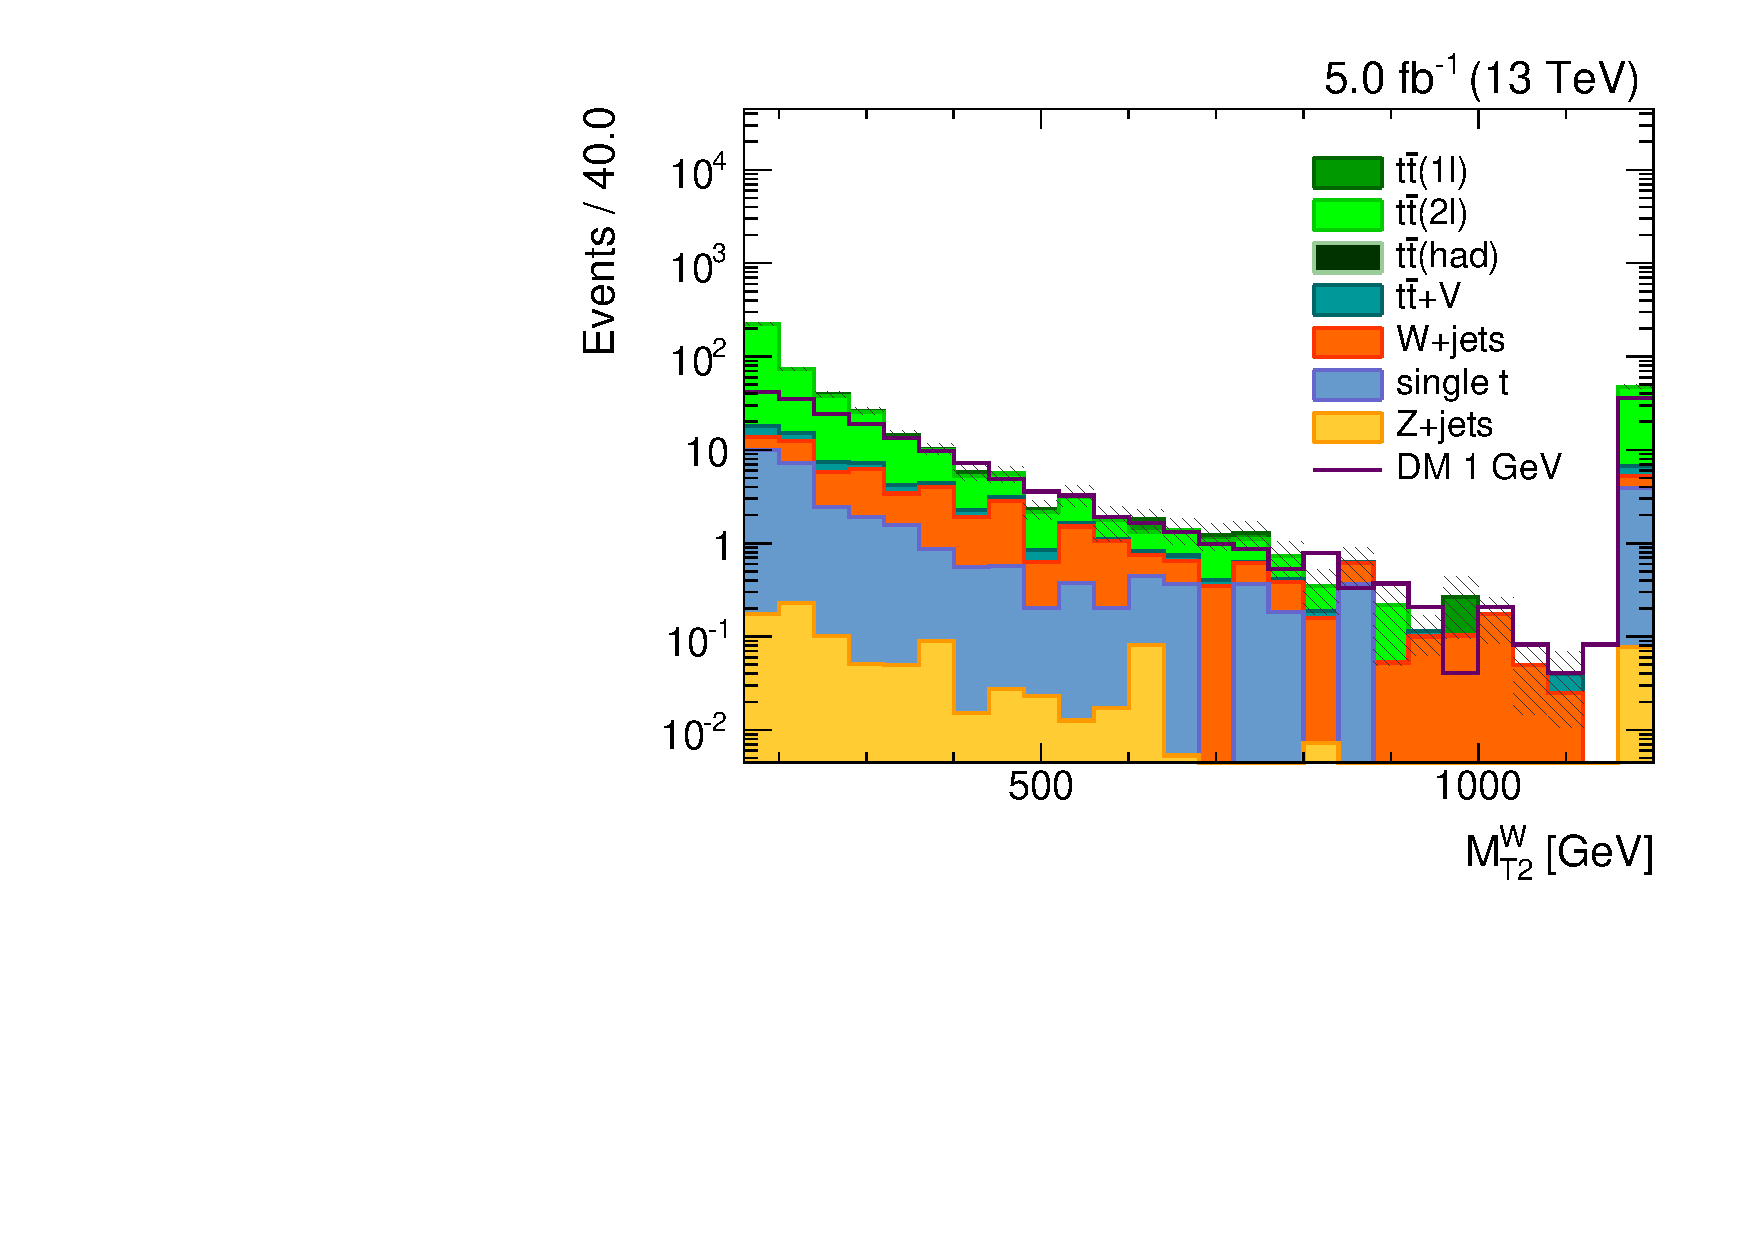
\includegraphics[width=0.48\textwidth]{figures/semilept-incl-mt2wlog_l.pdf}
  \caption{The $M_{T2}^W$ distribution in linear (left) and log (right) scales. Note that the right-most bin includes overflow.}
  \label{fig:incl_semilept_mt2w}
\end{figure}

\begin{figure}[htbp]
  \centering
  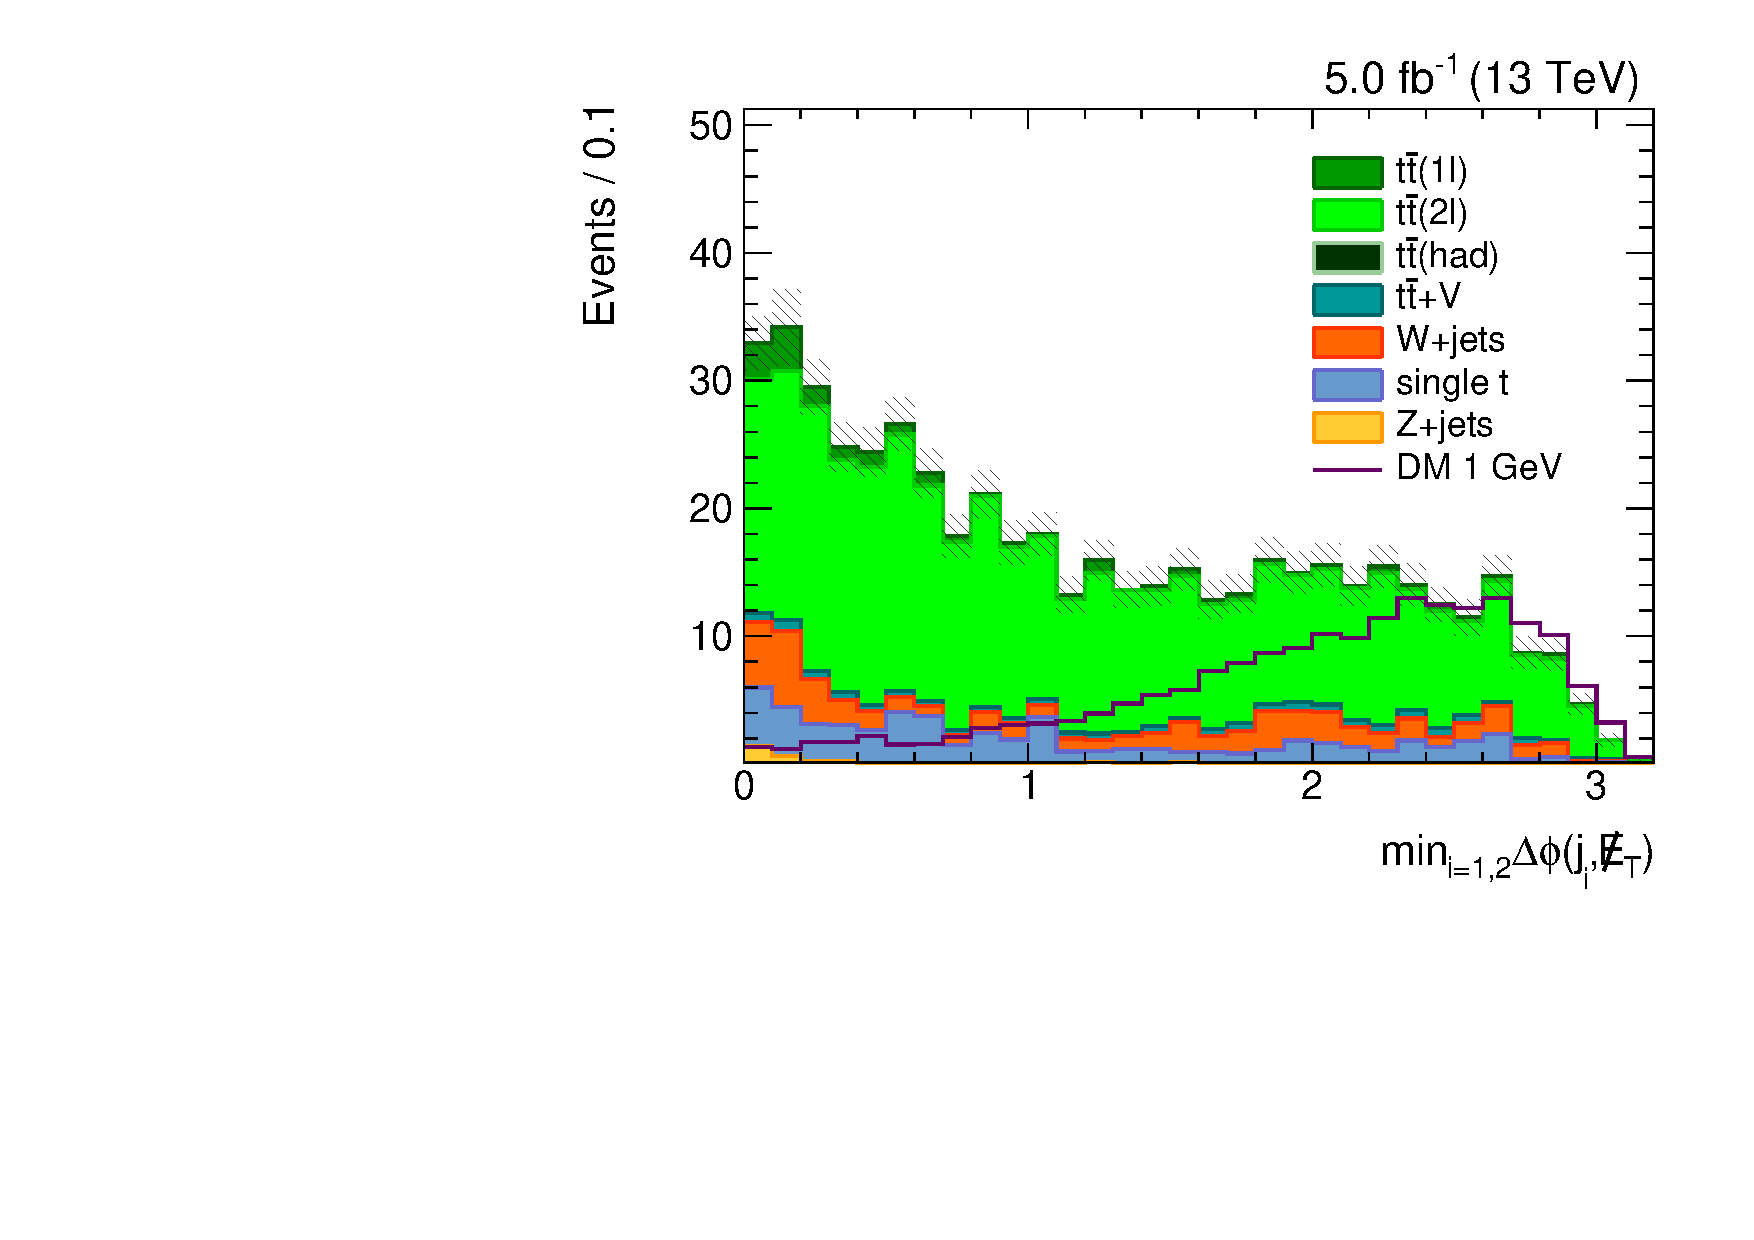
\includegraphics[width=0.48\textwidth]{figures/semilept-incl-dphijetmet2_l.pdf}
  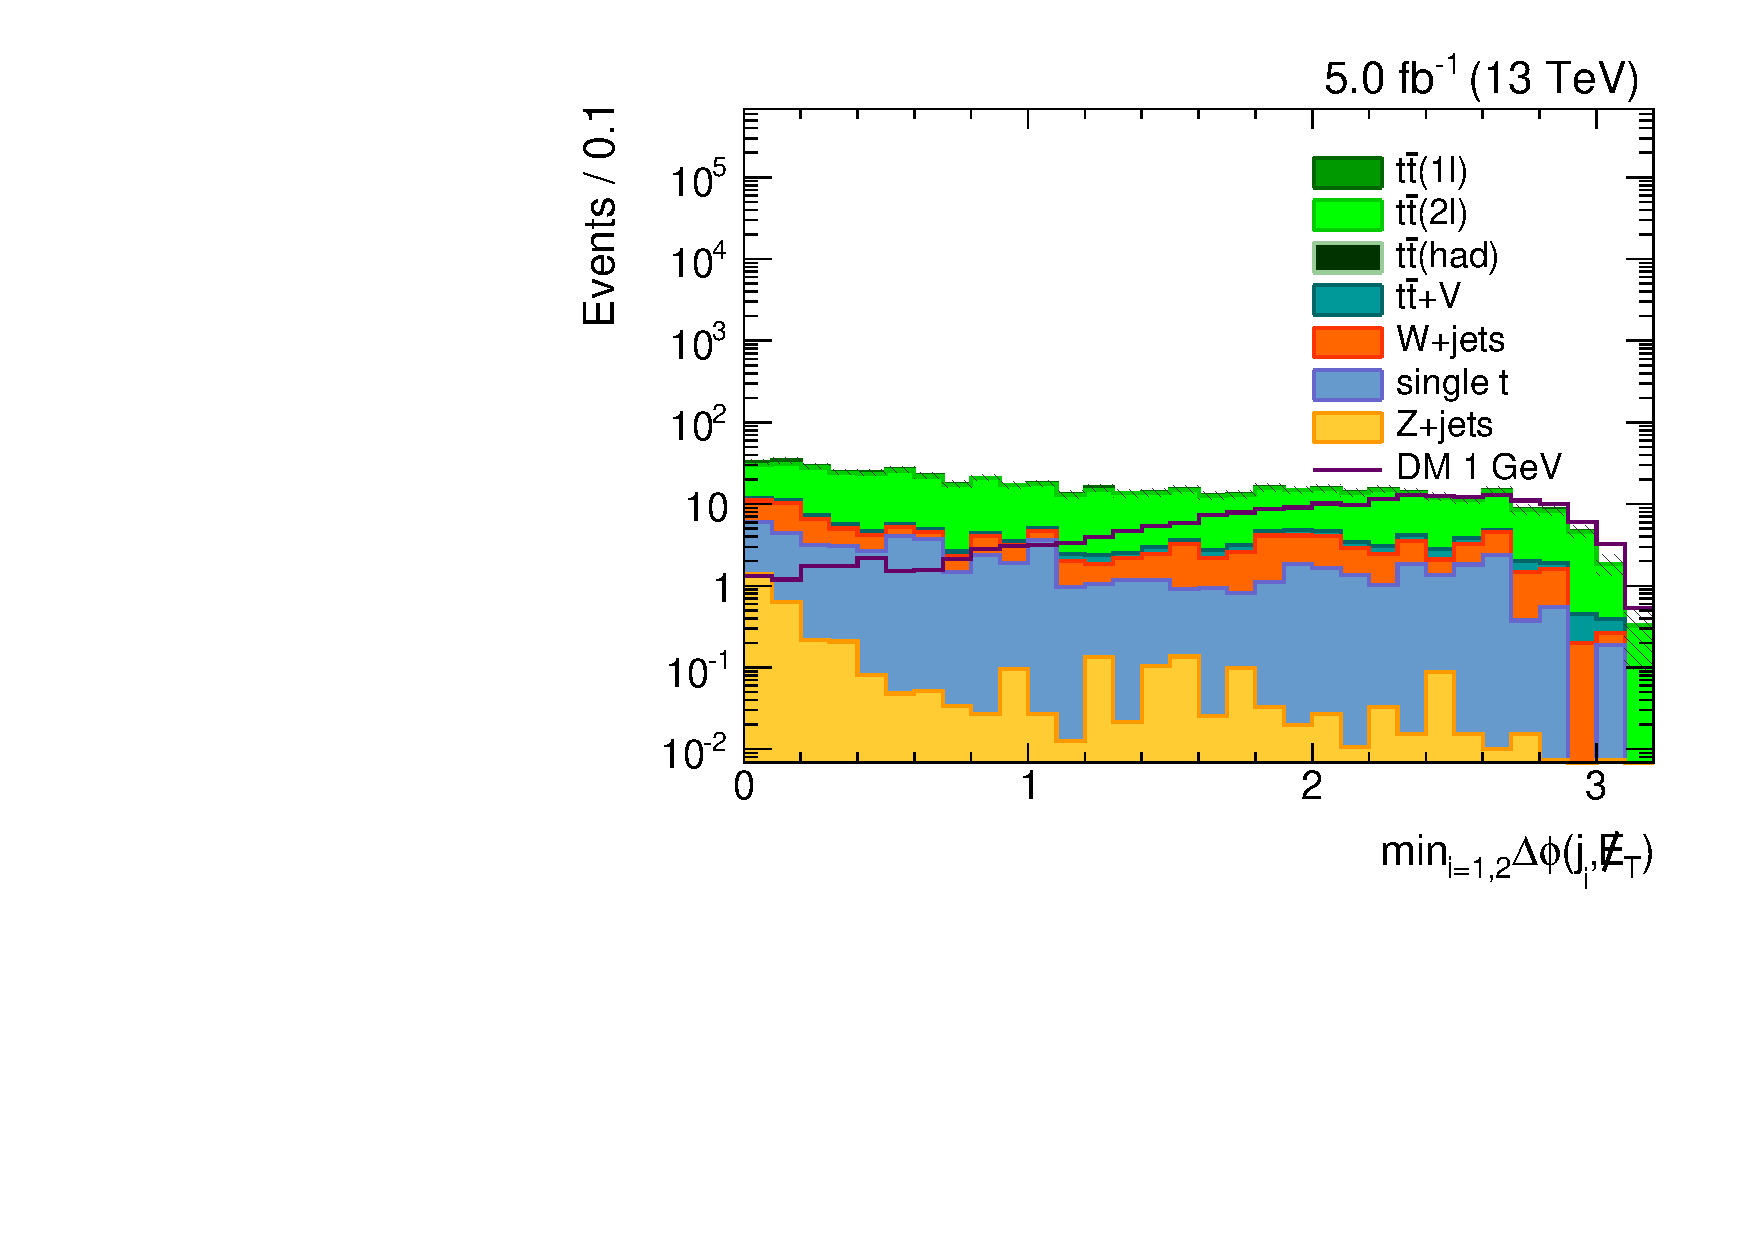
\includegraphics[width=0.48\textwidth]{figures/semilept-incl-dphijetmet2log_l.pdf}
  \caption{The $\min_{i=1,2}\Delta\phi\left(j_i\,\met\right)$ distribution in linear (left) and log (right) scales.}
  \label{fig:incl_semilept_dphijetmet2}
\end{figure}

The $\met$ distribution after selection is shown in Fig.~\ref{fig:incl_semilept_met}.
\begin{figure}[htbp]
  \centering
  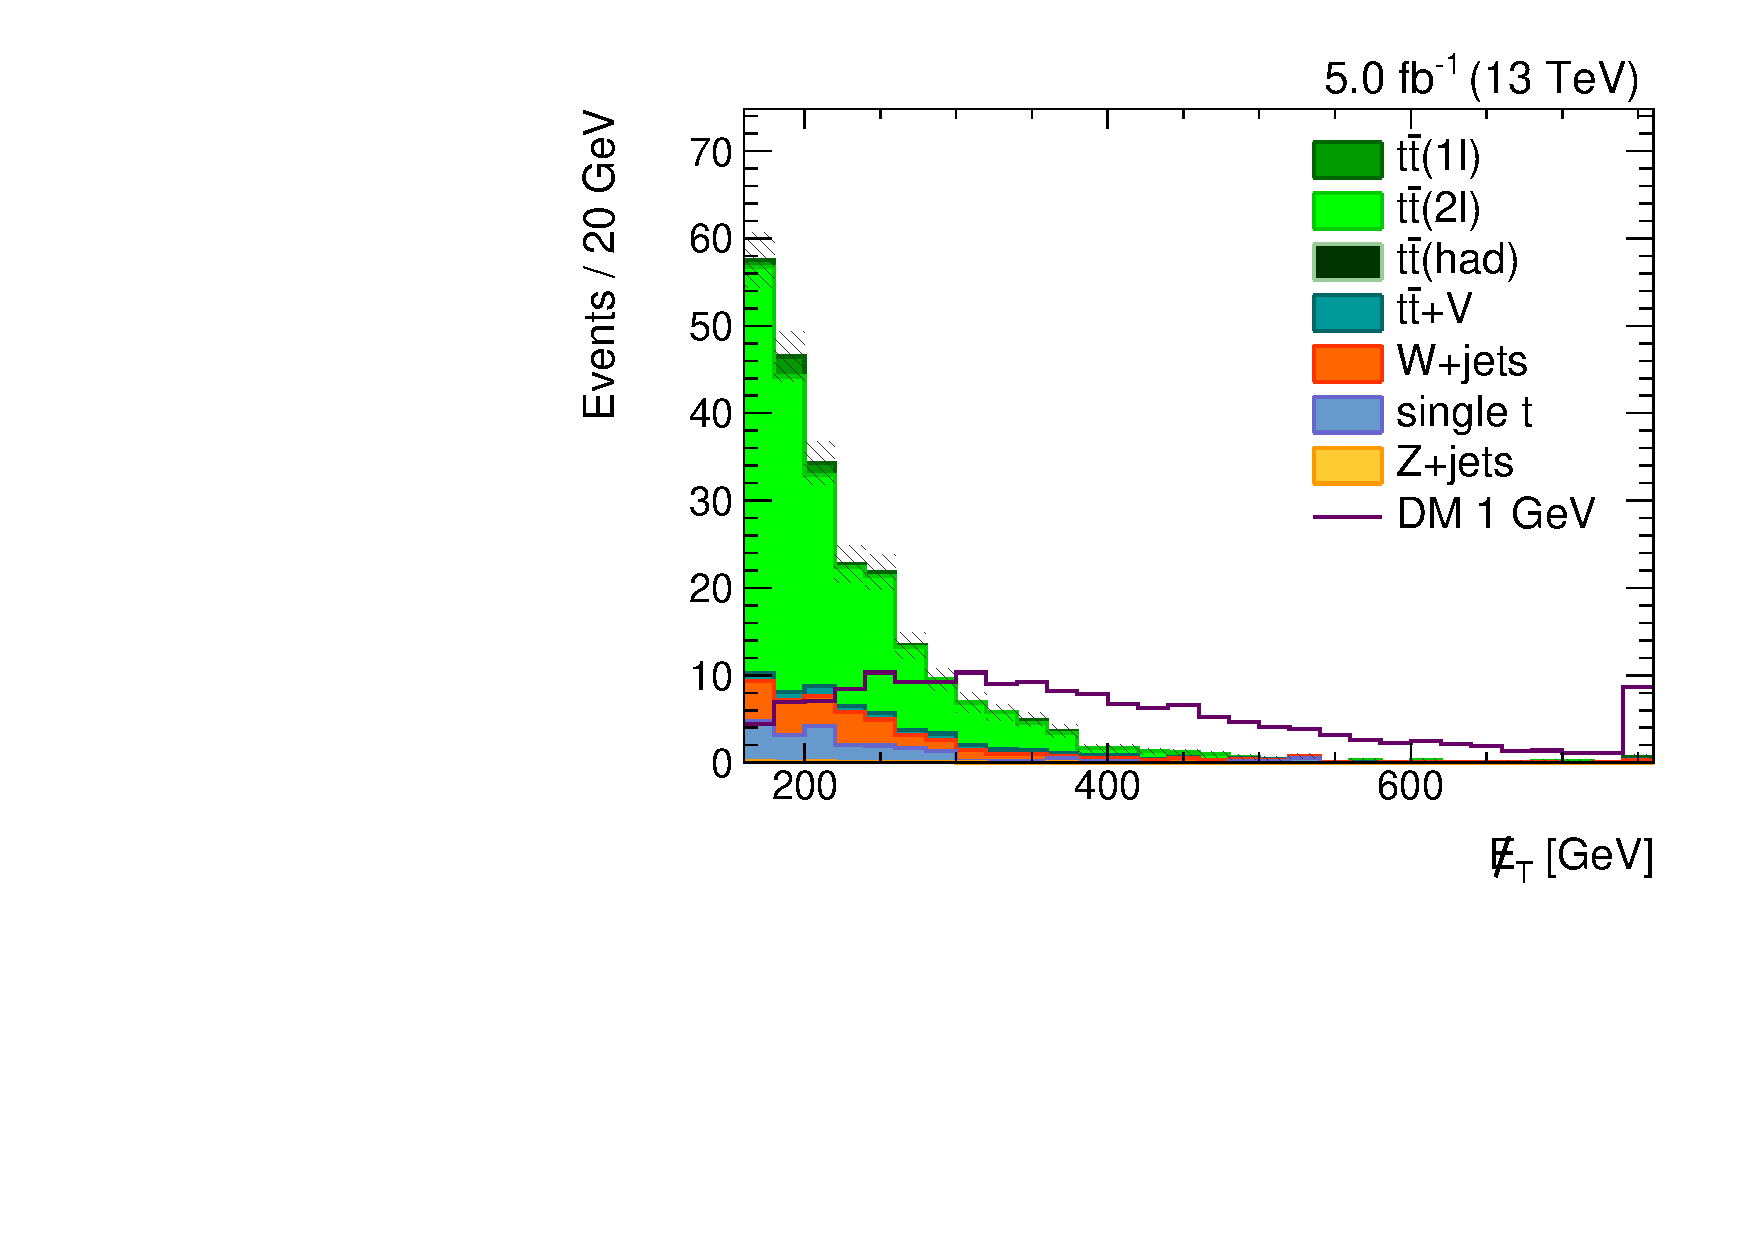
\includegraphics[width=0.48\textwidth]{figures/semilept-incl-met_l.pdf}
  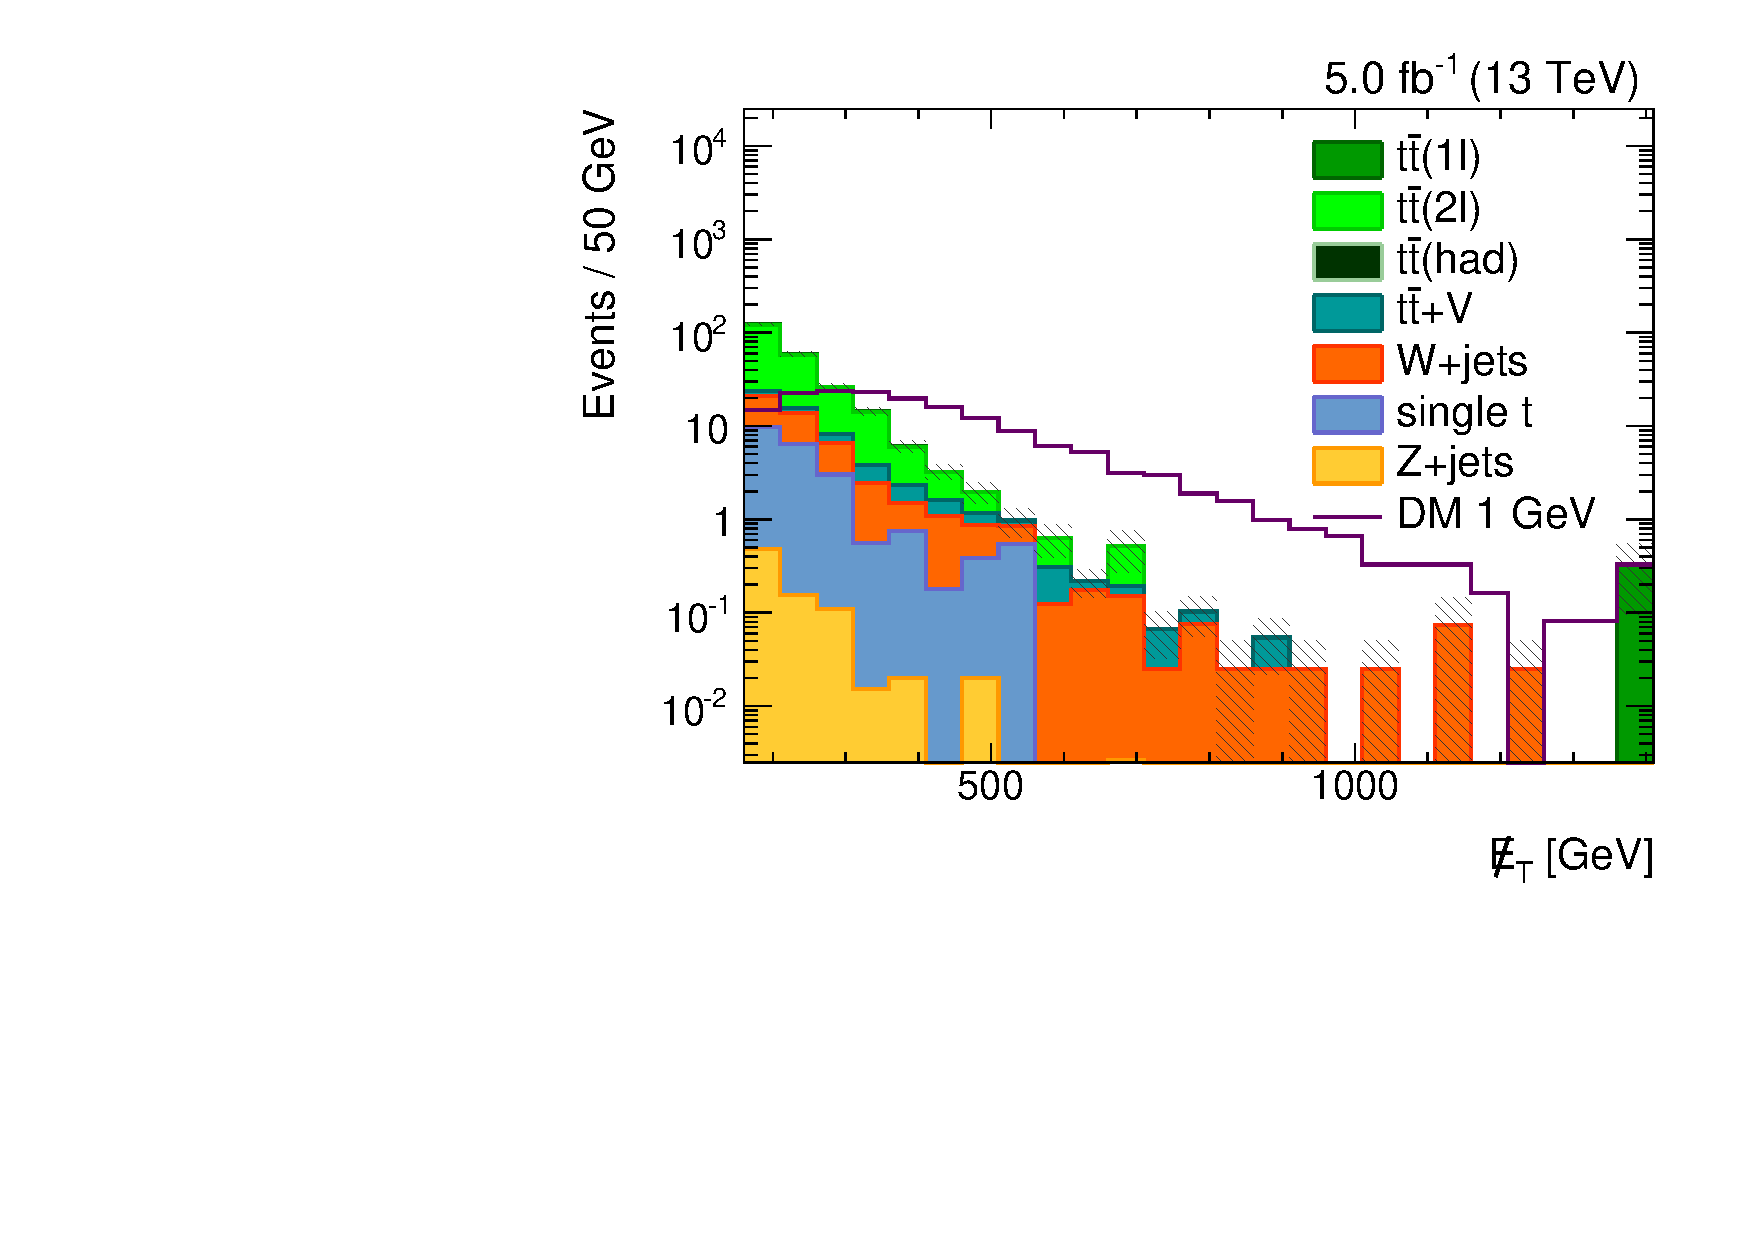
\includegraphics[width=0.48\textwidth]{figures/semilept-incl-metlog_l.pdf}
  \caption{The $\met$ distribution after semileptonic selection in linear (left) and log (right) scales. Note that the right-most bin includes overflow.}
  \label{fig:incl_semilept_met}
\end{figure}

The expected yields for $5\:\ifb$ after selection are shown in Table~\ref{tab:incl_semilept_yields}.

\begin{table}[!ht]
\centering
\begin{tabular}{|c|rr|r|}
\hline
  Process & \multicolumn{1}{|c}{$e$} & \multicolumn{1}{c|}{$\mu$} & \multicolumn{1}{|c|}{$e+\mu$} \\
\hline
  \Z\To\Lep\Lep         & $  0.28 \pm 0.09$ & $  0.52 \pm 0.14$ & $  0.80 \pm 0.17$ \\
  Single \Top           & $  7.75 \pm 1.18$ & $ 13.01 \pm 1.53$ & $ 20.76 \pm 1.93$ \\
  \Wjets                & $ 11.23 \pm 1.57$ & $ 16.31 \pm 2.35$ & $ 27.54 \pm 2.83$ \\
  $\ttbar+V$            & $  4.22 \pm 0.24$ & $  5.27 \pm 0.27$ & $  9.50 \pm 0.37$ \\
  $\ttbar\mbox{(had)}$  & $  0.00 \pm 0.00$ & $  0.00 \pm 0.00$ & $  0.00 \pm 0.00$ \\
  $\ttbar(2\Lep)$       & $ 77.30 \pm 3.55$ & $ 95.61 \pm 3.95$ & $172.91 \pm 5.32$ \\
  $\ttbar(1\Lep)$       & $  3.43 \pm 0.75$ & $  2.78 \pm 0.67$ & $  6.21 \pm 1.01$ \\

\hline
  SM expected           & $365.94 \pm 4.14$ & $133.50 \pm 4.91$ & $237.72 \pm 6.42$ \\
\hline
  $M_\chi=1\:\GeV$      & $289.61 \pm 1.75$ & $ 91.77 \pm 1.94$ & $165.93 \pm 2.61$ \\
\hline
\end{tabular}
\caption{Expected yields for $5\:\ifb$ after the inclusive selection for the semileptonic channel.}
\label{tab:incl_semilept_yields}
\end{table}

%\subsection{Boosted Top Tagging}
\label{subsec:sel_toptag_boosted}

Jet substructure techniques can be used to identify boosted top decays where all the decay products are contained within a single jet. Wider jets are considered so that substructure methods are applicable for tops with moderate boost. In this analysis, jets with $R=1.5$ are considered so that tops with $\pt>250\:\GeV$ are fairly well contained within the jet. Soft drop jet grooming, $N$-subjettiness, and subjet $\Bot$-tagging are applied to tag top decays.

By analyzing the radiation pattern within a jet, it is possible to differentiate between a jet induced by a single parton and a jet induced by the decay of a massive particle. The soft drop algorithm removes soft, wide angled radiation and decomposes a jet into subjets that correspond to the underlying hard partons that induce the jet. The settings used for soft drop are $\beta=0$ and $z_{\mbox{\scriptsize{cut}}}=0.1$. The soft drop mass ($M_{\mbox{\scriptsize{soft drop}}}$) spectrum is shown in Fig.~\ref{fig:softdrop}, for events with a single ``Tight'' muon or electron, $M_T>160\:\GeV$, and at least one AK4CHS $\Bot$-tagged jet.

\begin{figure}[htbp]
  \centering
  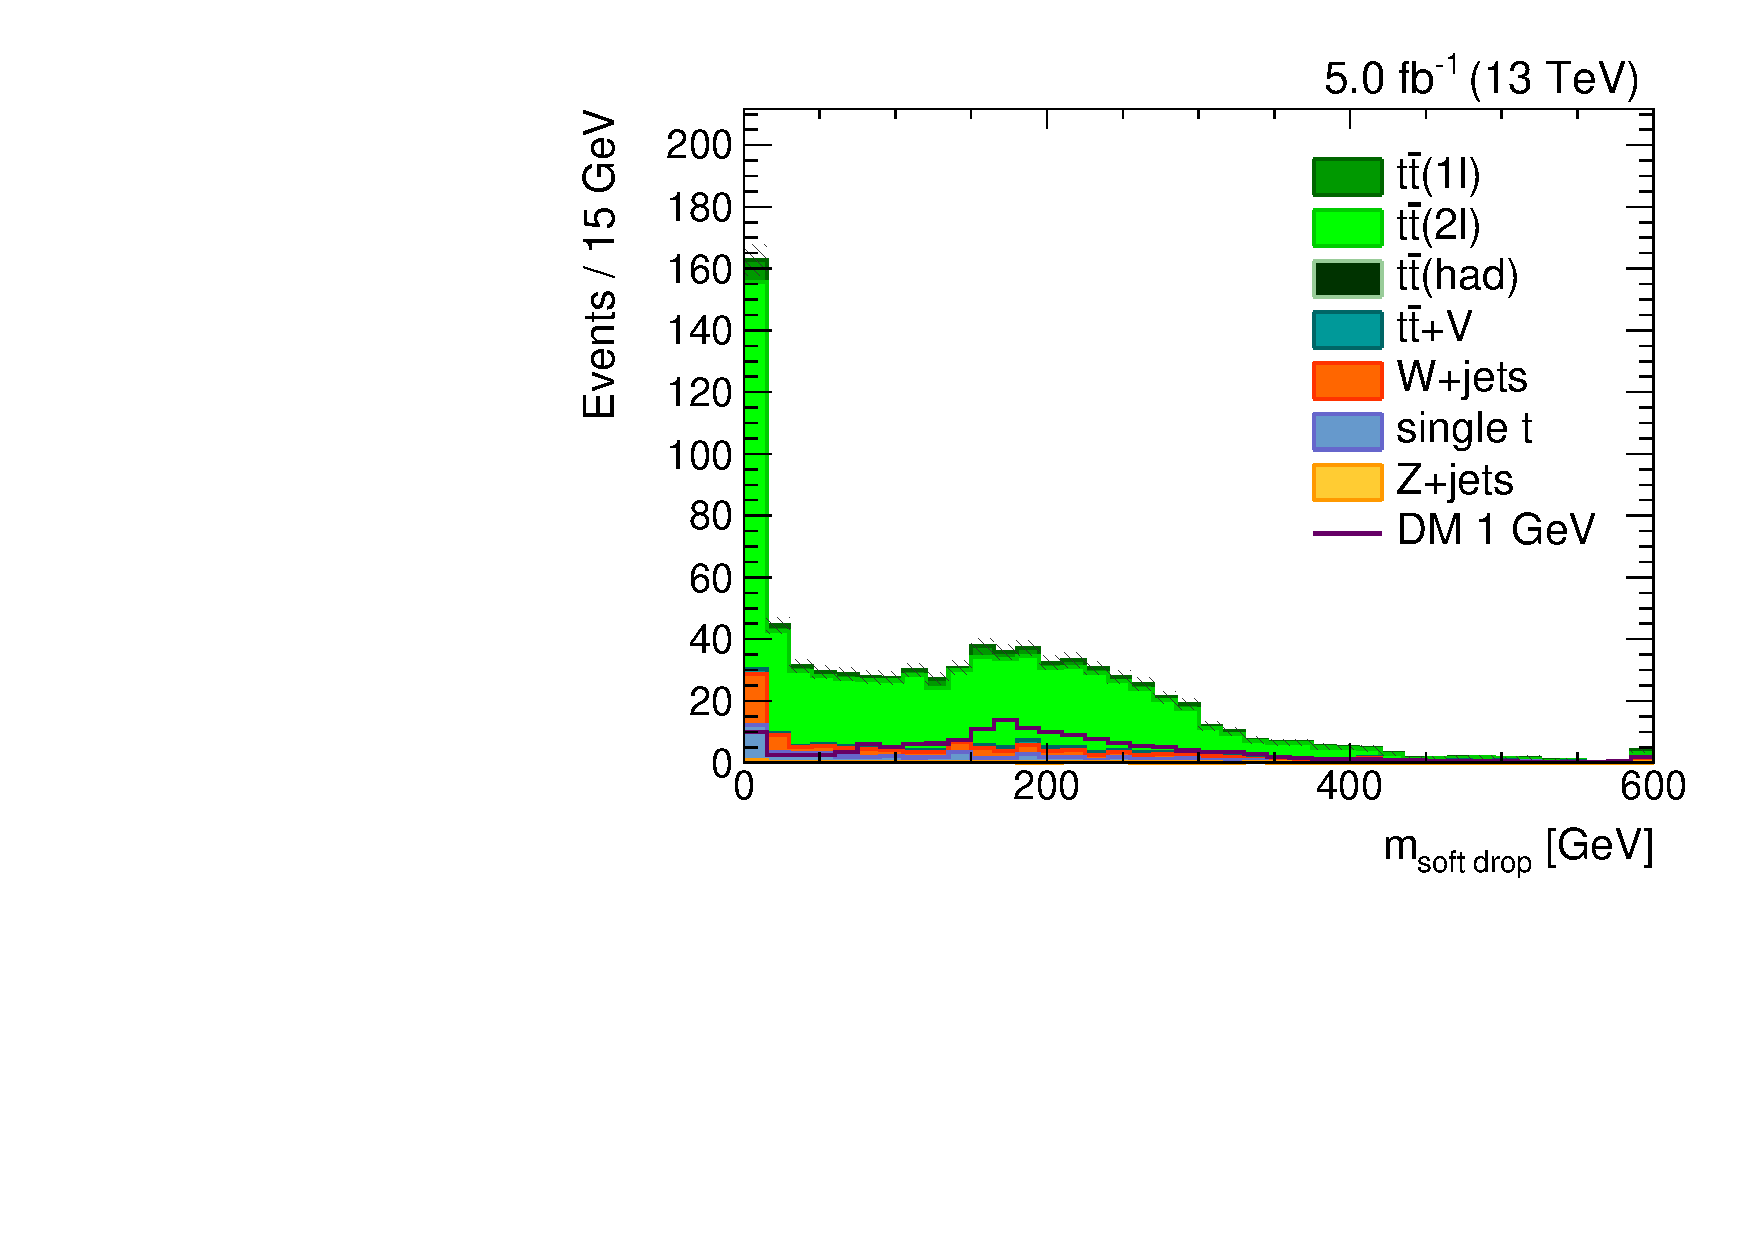
\includegraphics[width=0.48\textwidth]{figures/softdrop.pdf}
  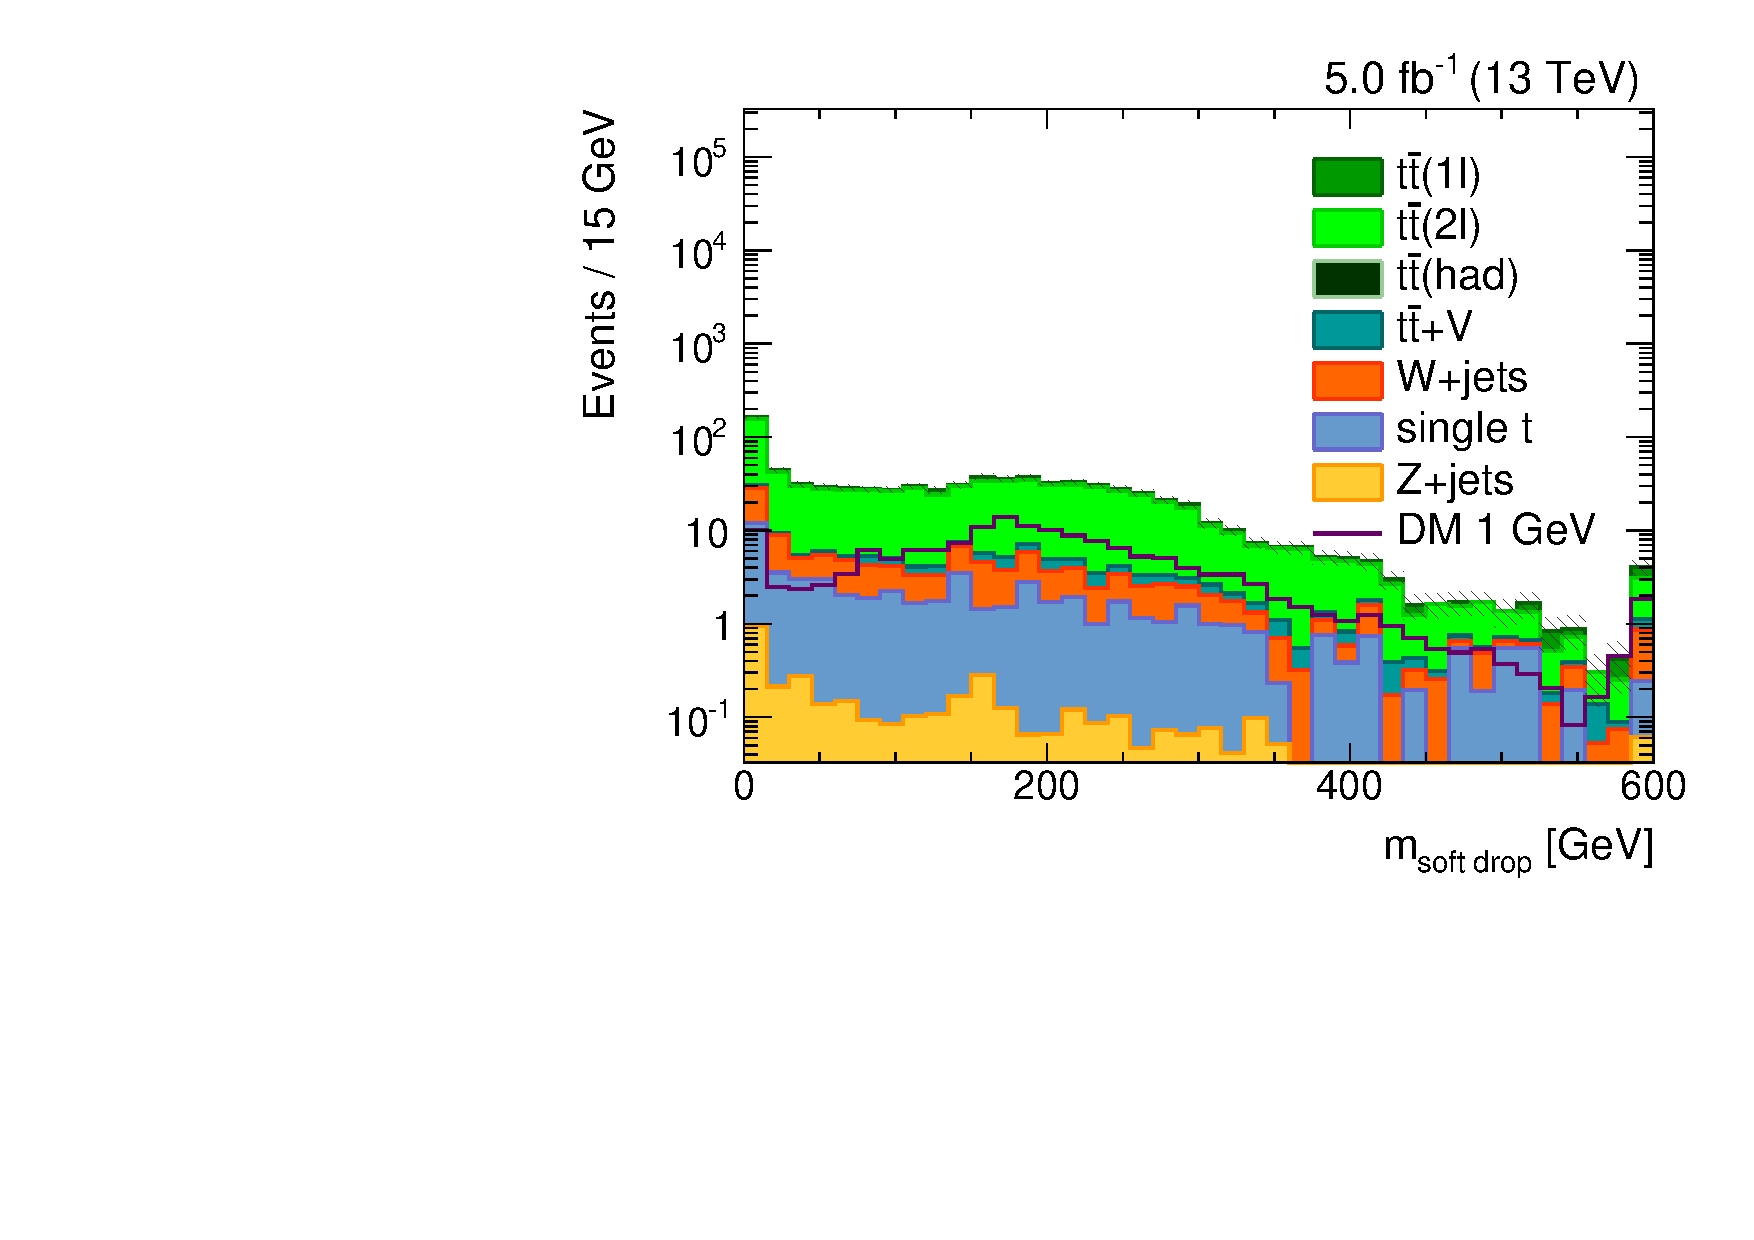
\includegraphics[width=0.48\textwidth]{figures/softdroplog.pdf}
  \caption{Jet mass distribution after grooming with the soft drop ($\beta=0, z_{\mbox{\scriptsize{cut}}}=0.1$) algorithm.}
  \label{fig:softdrop}
\end{figure}

$N$-subjettiness quantifies the likelihood a jet comprises of $N$ or more prongs. The discriminating variable is the ratio of $N$-subjettiness quantities; in particular, the $\tau_n/\tau_{n-1}$ ratio quantifies the likelihood the jet comprises of $n$ prongs. Hence, $\tau_3/\tau_2$ is used to help identify top decays. The $\tau_3/\tau_2$ distribution for events with $M_{\mbox{\scriptsize{soft drop}}}>75\:\GeV$ is shown in Fig.~\ref{fig:tau32}.

\begin{figure}[htbp]
  \centering
  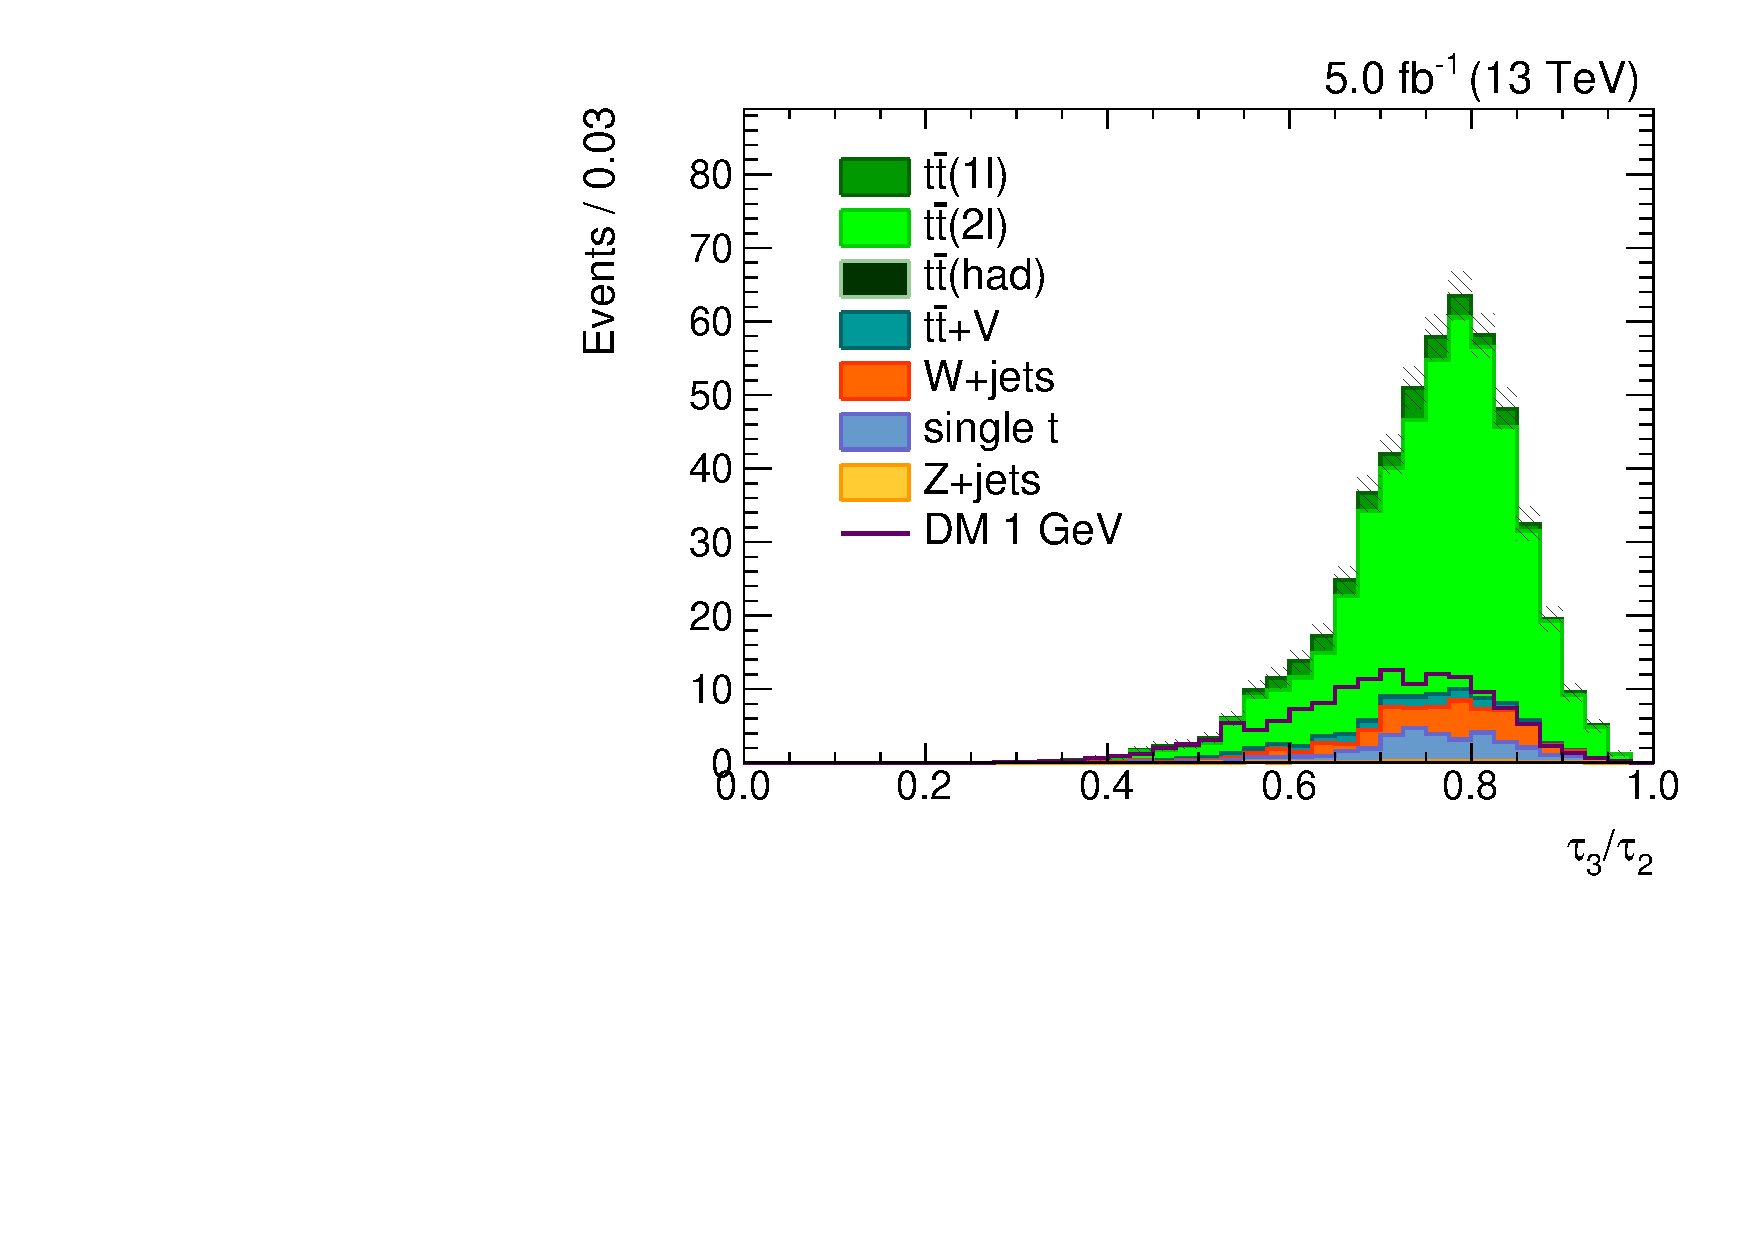
\includegraphics[width=0.48\textwidth]{figures/tau32.pdf}
  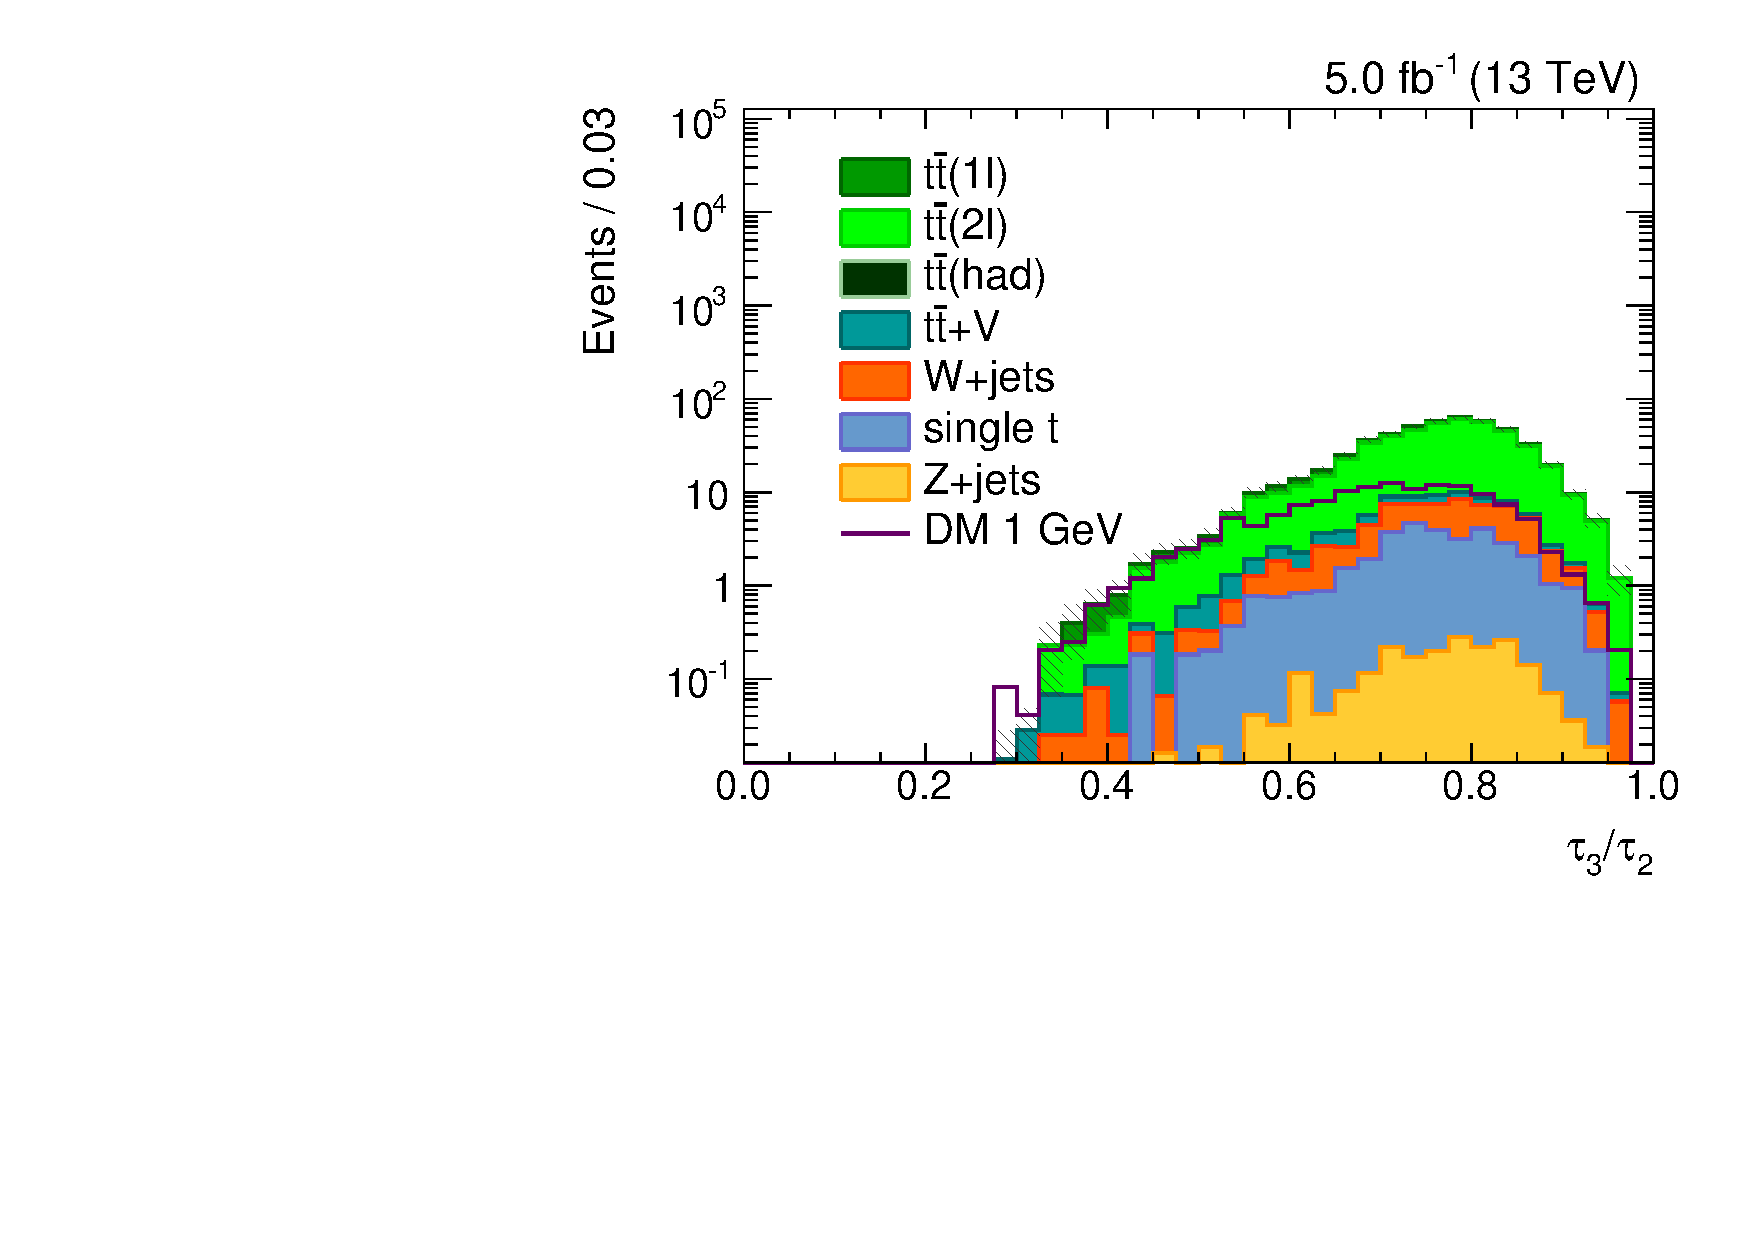
\includegraphics[width=0.48\textwidth]{figures/tau32log.pdf}
  \caption{Distribution of $\tau_3/\tau2$ for jets with $M_{\mbox{\scriptsize{soft drop}}}>75\:\GeV$.}
  \label{fig:tau32}
\end{figure}

The $\Bot$ quark from the top decay is expected to be contained in the wide jet and therefore the corresponding subjet should have properties similar to typical $\Bot$-jets. The CSVv2+IVF $\Bot$-tag algorithm is performed on subjets from the soft drop decomposition to provide further discrimination for top decays. The distribution for the largest $\Bot$-tag value among subjets in a jet, for jets with $M_{\mbox{\scriptsize{soft drop}}}>75\:\GeV$, is shown in Fig.~\ref{fig:subjet_btag}.

\begin{figure}[htbp]
  \centering
  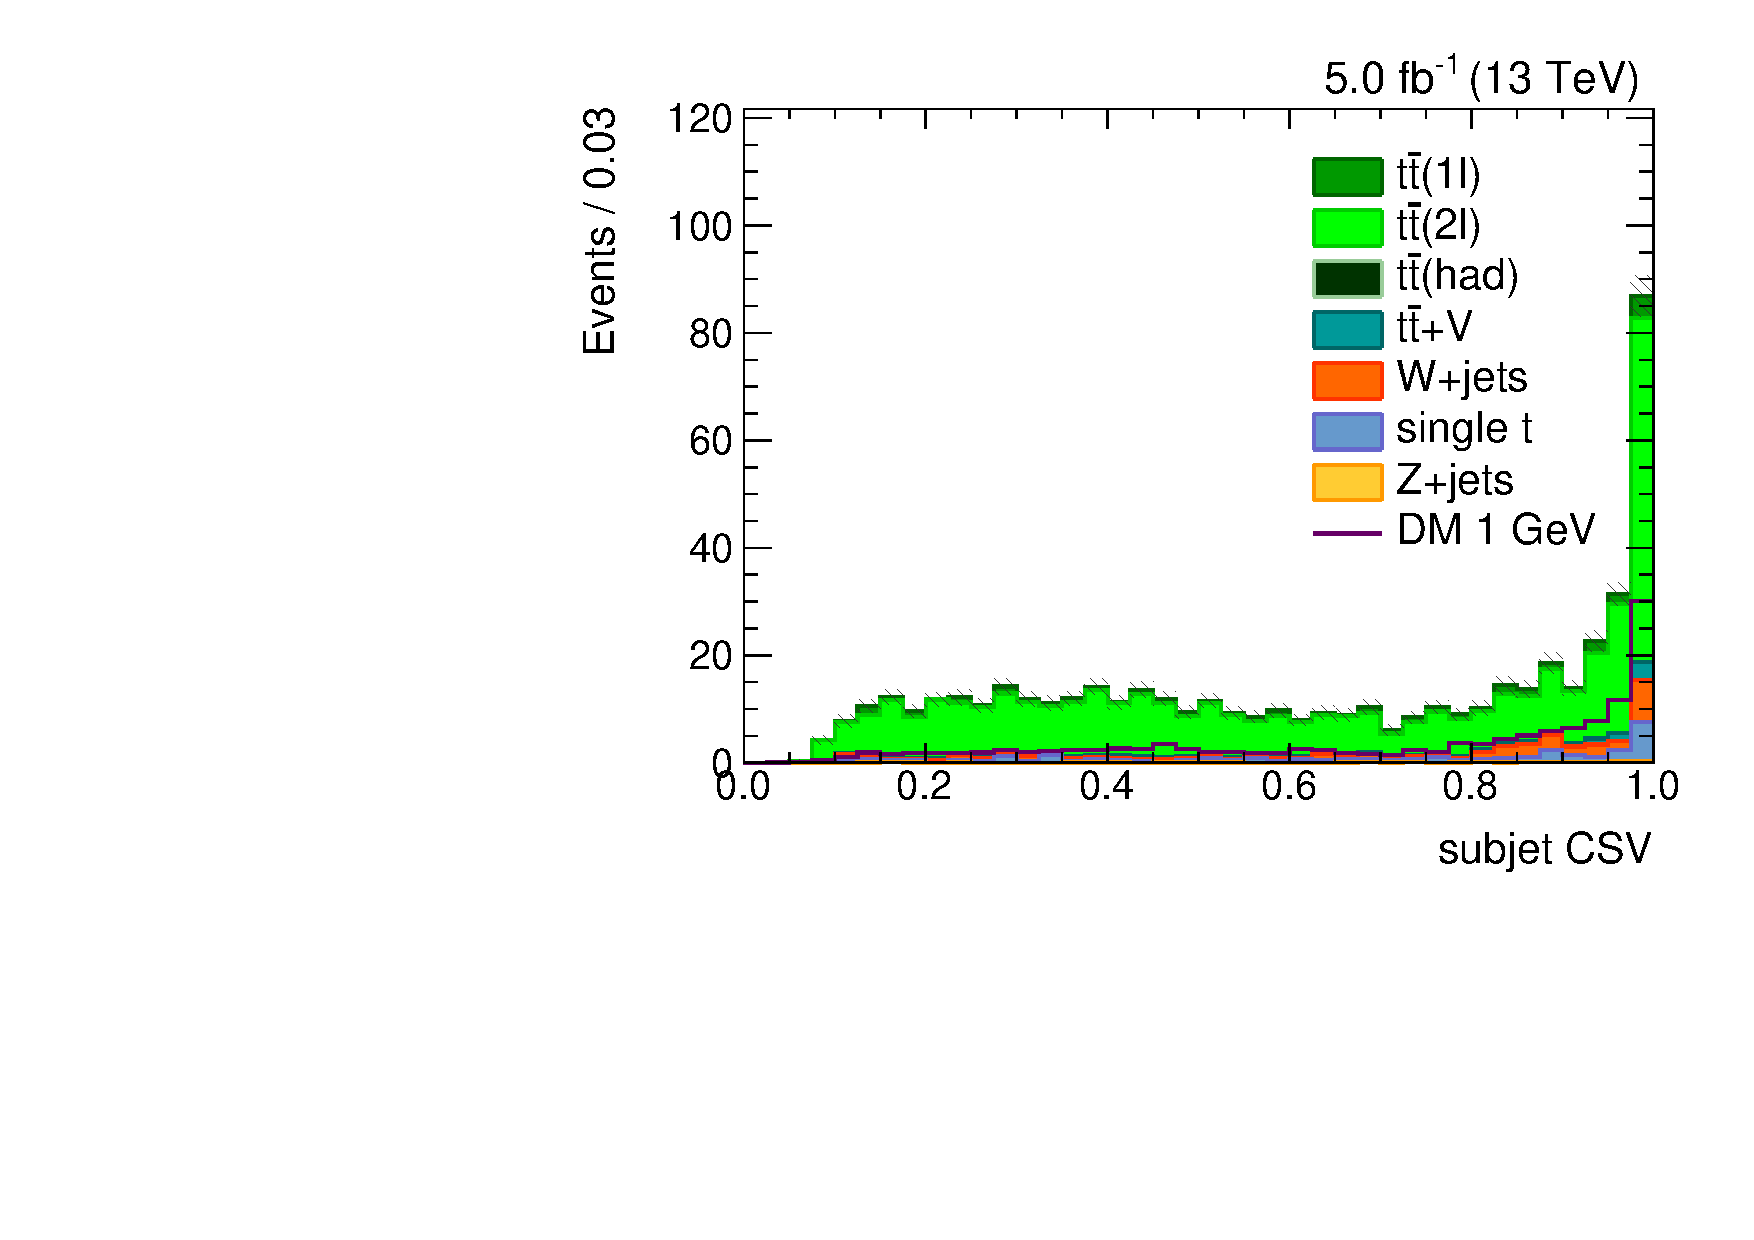
\includegraphics[width=0.48\textwidth]{figures/subjetbtag.pdf}
  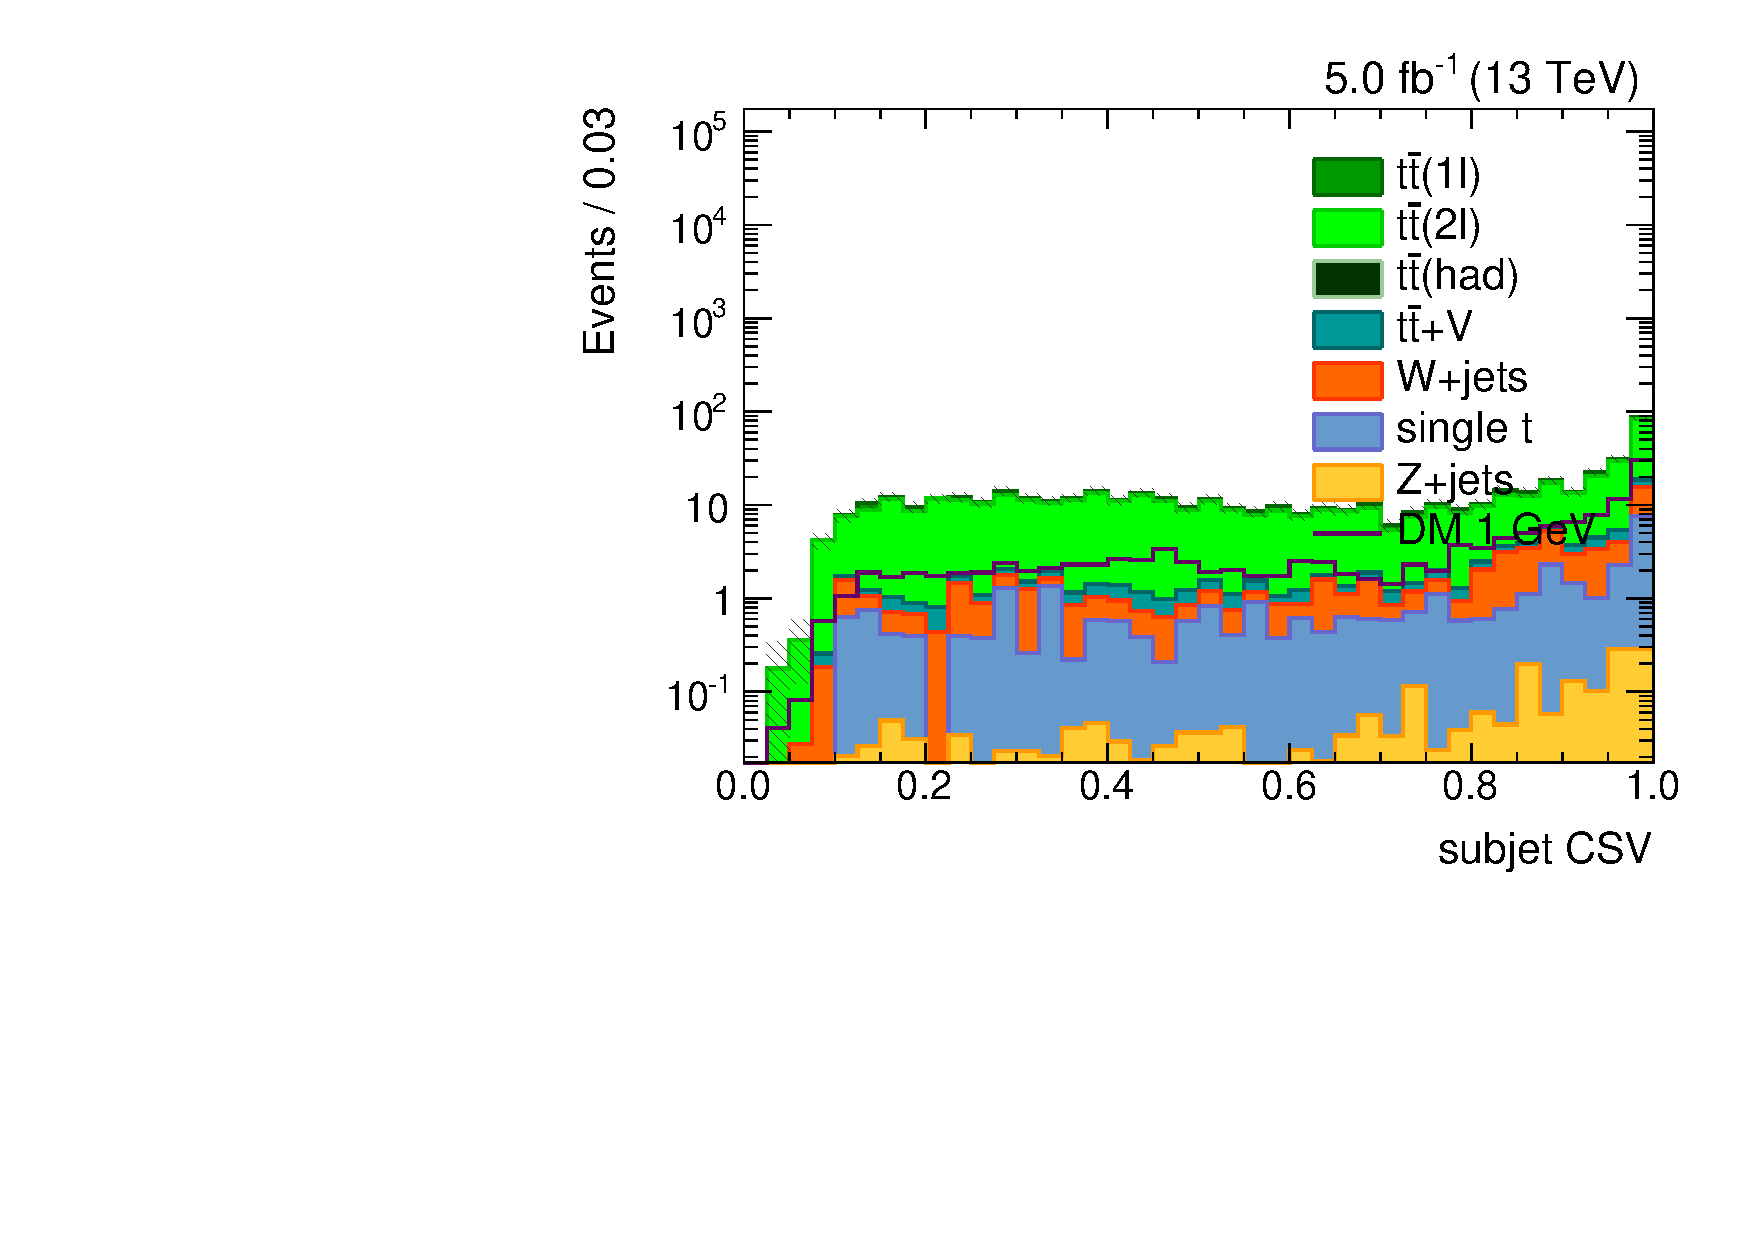
\includegraphics[width=0.48\textwidth]{figures/subjetbtaglog.pdf}
  \caption{Distribution of the largest CSVv2+IVF value among subjets in a wide jet. The wide jet must have $M_{\mbox{\scriptsize{soft drop}}}>75\:\GeV$.}
  \label{fig:subjet_btag}
\end{figure}

A boosted top is identified by the following requirements, 
\begin{itemize}
\item CA15CHS jet with $\pt>250\:\GeV$ and $|\eta|<2.4$,
\item $M_{\mbox{\scriptsize{soft drop}}} > 75\:\GeV$
\item $\tau_3/\tau_2 < 0.75$
\item maximum subjet $\Bot$-tag $> 0.4$
\end{itemize}

\clearpage
\subsection{Resolved Top Tagging}
\label{subsec:sel_toptag_resolved}

This analysis relies on the identification of resolved top decays. The resolved top decays are defined as consisting of three jets, each separately clustered by the anti-$k_{T}$ algorithm with size parameter R = 0.4. These AK4CHS jets employ charged hadron subtraction to reduce pileup contamination. Each jet is required to have a $\pt$ of at least $30\:\GeV$ and be located within the detector volume.

The resolved top tagging tool used in this analysis is a boosted decision tree (BDT) based multivariate discriminator (MVA), trained using the \textit{Toolkit for Multivariate Data Analysis with ROOT} (TMVA version 4.2.0) \cite{tmva}. The events selected for MVA training are from SM $\ttbar$ processes simulated in the Phys14 MC sample TTJets\_MSDecaysCKM\_central\_Tune4C\_13TeV-madgraph-tauola with a total cross-section of 831.76 pb. We use single lepton $\ttbar$ events and focus on the top where the W boson decays hadronically into two quarks which fragment and hadronize into jets. We permute all combinations of three jets from each event. Each jet from the tri-jet com bination is matched to a generator level parton which is within $\Delta R$ = 0.3 of the jet. 

The training of the MVA exploits the properties of the resolved top decay kinematics and jet identification properties. The jet properties used in the MVA training include a b-tagging discriminant value. This is determined via the most recent version of the \textit{Combined Secondary Vertex} algorithm (v2) together with the \textit{Inclusive Vertex Finder} algorithm (CSVv2+IVF). Although no explicit cut is applied on the b-tag discriminant for the selection of training events, we denote the jet with the highest CSVv2+IVF value as the b jet candidate. The remaining two jets are denoted as candidates for the jets emitted by the hadronic decay of the W boson. Other variables used in the training include the \textit{Quark-Gluon Likelihood} value of each jet, a value that corresponds to whether a jet originated from a quark or a gluon. The opening angles between the resolved top decay jets are also used. These include the separation in $R$- and $\phi$-space between each W decay jet candidate and the b jet candidate. 

We also employ a kinematic fit to the selected combination of three jets, and from this extract a fit probability \cite{kinfit}. We consider the invariant mass of the system comprised of the two candidate jets for the hadronic decay of the W boson. We also consider the three-jet system which includes the b jet candidate. The invariant masses of the two- and three-jet systems are constructed and the four-vectors of the jets are allowed to vary within their respective uncertainties in order to satisfy the top quark and W boson mass constraints imposed. A minimized $\chi^{2}$ function is extracted from the convergence of the kinematic fit and translated into a probability of fit. 

The input variables used in the training of the resolved top tagger include:
\begin{itemize}
\item jet CSVv2+IVF
\item jet quark-gluon likelihood (QGL)
\item $\Delta R$ ( hadronic W decay jet$_{\mbox{\scriptsize{1,2}}}$, b jet )
\item $\Delta \phi$ ( hadronic W decay jet$_{\mbox{\scriptsize{1,2}}}$, b jet )
\item fit probability 
\end{itemize}

and the jets selected for training satisfy the following requirements: 
\begin{itemize}
\item 3 AK4CHS jets with $\pt>30\:\GeV$ and $|\eta|<2.4$	
\item $100\:\GeV<M_{\mbox{\scriptsize{jjj}}}<300\: \GeV$
\end{itemize}

The MVA is trained with 100,000 signal events and 200,000 background events using the decision tree method which implements the \textit{GradientBoost} algorithm. A \textit{shrinkage} parameter, the learning rate for the GradientBoost algorithm, of 0.05 is specified. The small shrinkage necessitates the growth of more decision trees, but can significantly improve the accuracy of a prediction in difficult settings.

Input training variable correlations are shown in Fig.~\ref{fig:corr}. As expected, the kinematic angles $\Delta R$ and $\Delta\phi$ between the W decay candidate jets and the b jet candidate are correlated strongly in the signal, and less so in the background. 

\begin{figure}[htbp]
	\centering
	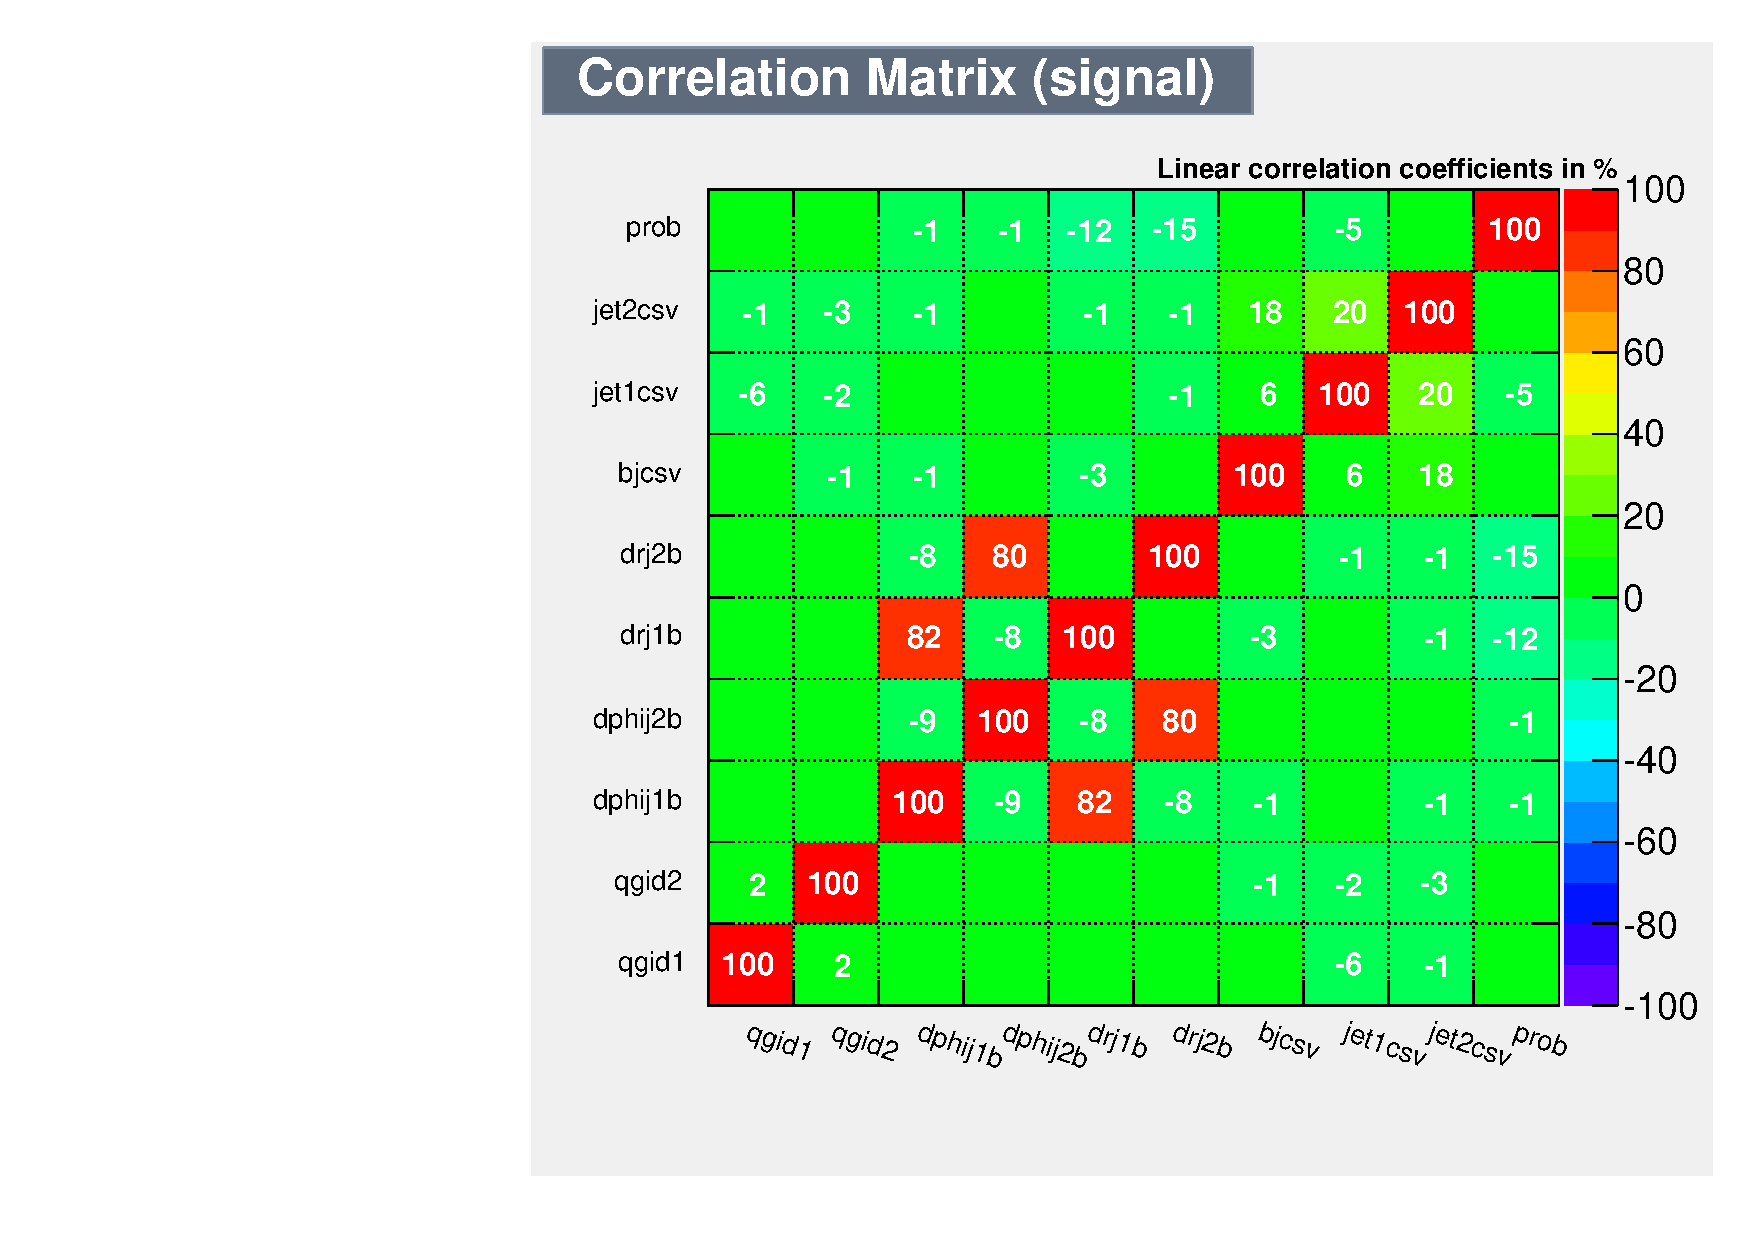
\includegraphics[width=0.48\textwidth]{figures/CorrelationMatrixS.pdf}
	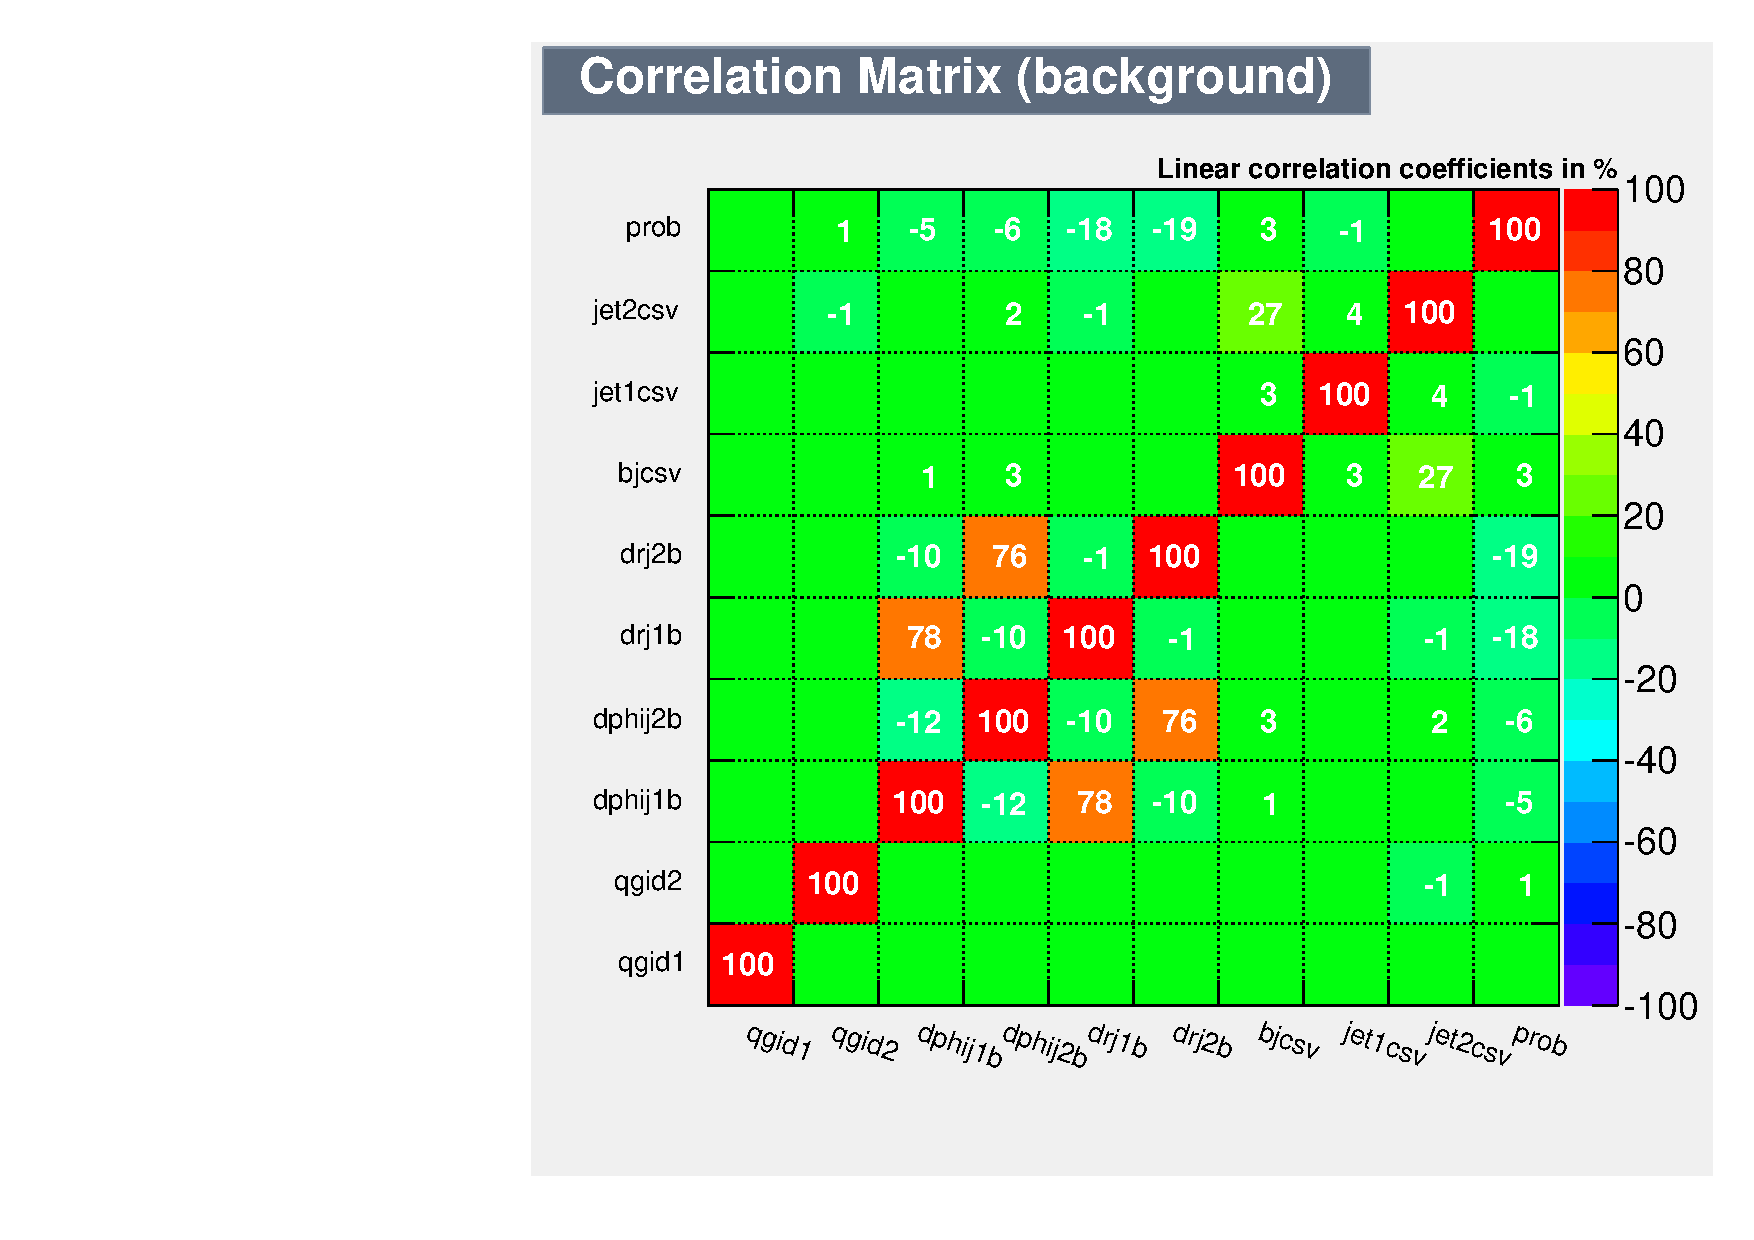
\includegraphics[width=0.48\textwidth]{figures/CorrelationMatrixB.pdf}
	\caption{Correlations between MVA input variables for signal and background}
	\label{fig:corr}
\end{figure}

The performance of the resolved top tagger is evaluated in single lepton $\ttbar$ events and $\Z\To\Nu\Nu$(+jets) events. Unique subsets of the same SM $\ttbar$ MC sample are used to train and test the MVA. A single event can contribute multiple background combinations, thus the tagger is evaluated using the background combination which has the highest output MVA score.

\begin{figure}[htbp]
	\centering
	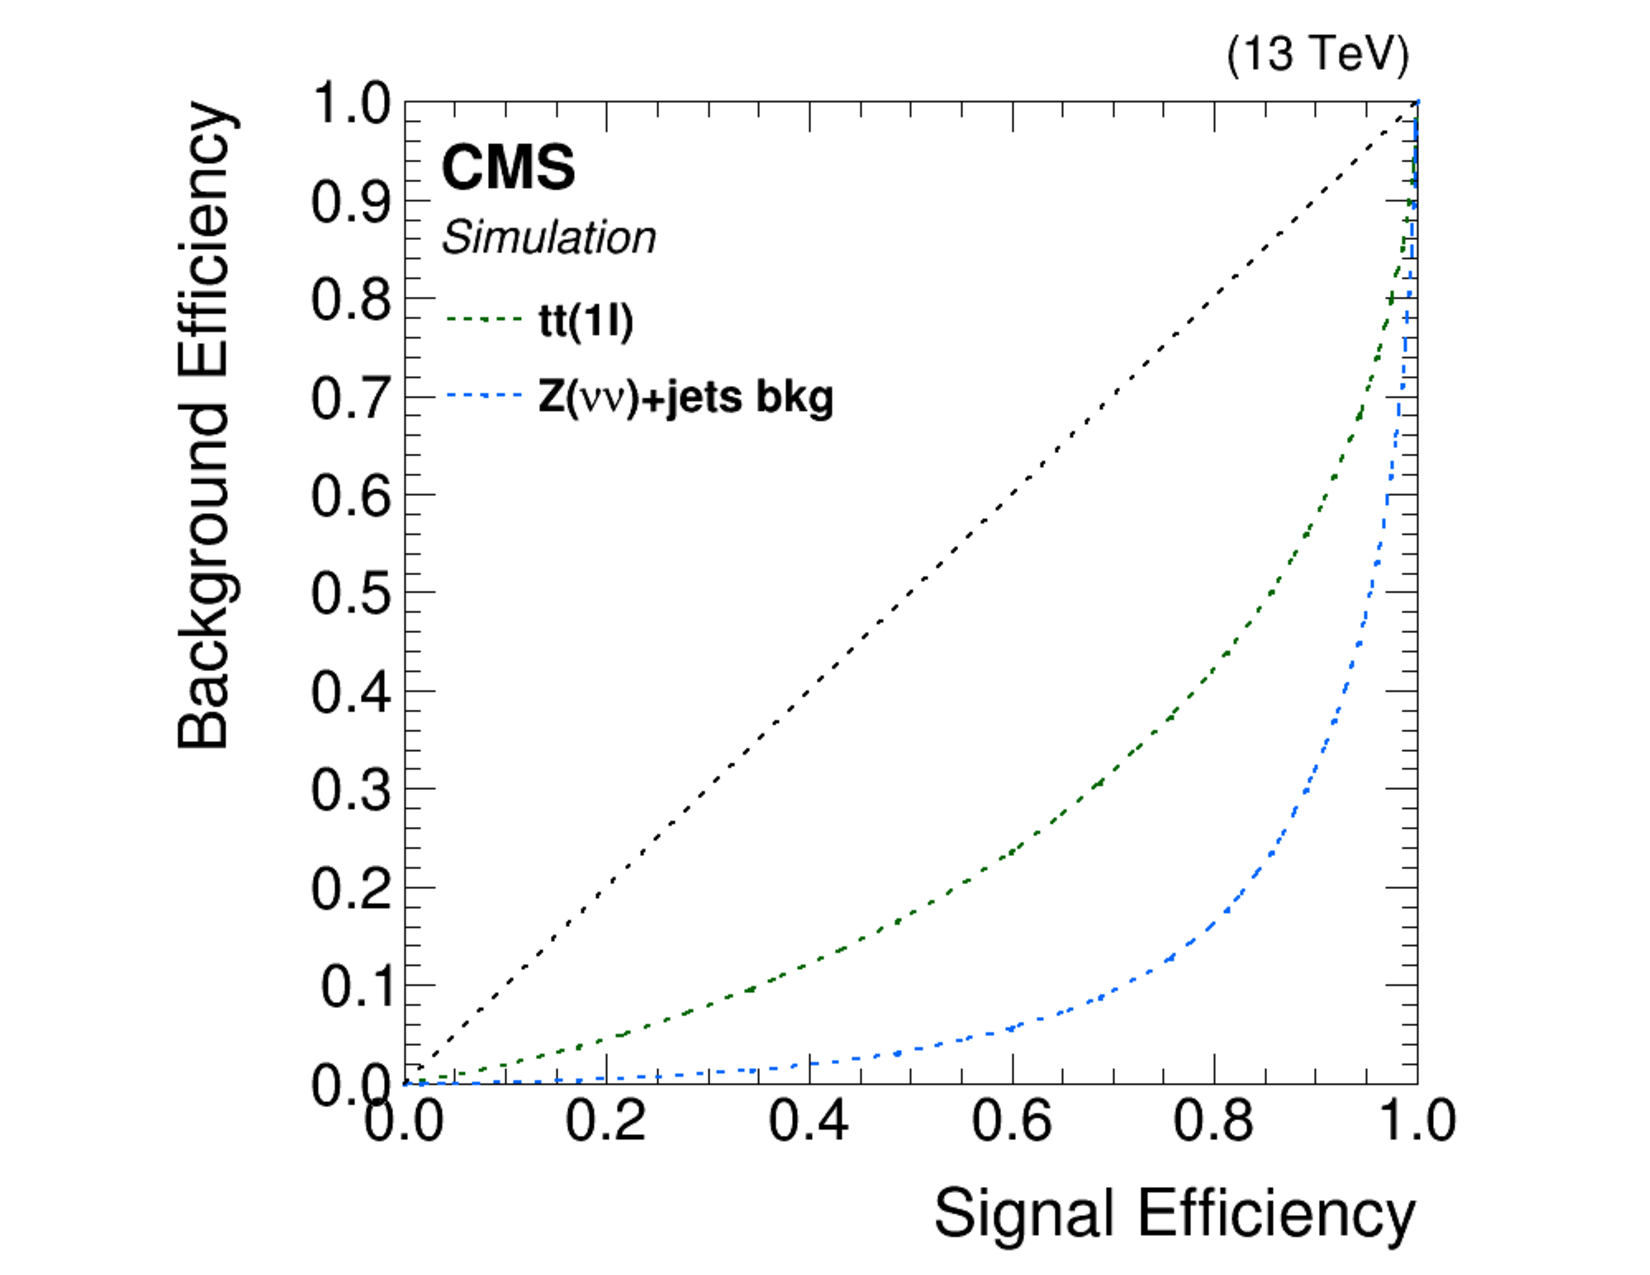
\includegraphics[width=0.48\textwidth]{figures/roctt1lzjets.pdf}
	\caption{Background  vs. signal efficiencies for $\ttbar(1\Lep)$ and $\Z\To\Nu\Nu$(+jets)}
	\label{fig:rocres}
\end{figure}

The efficiency behaviour of the resolved top tagger with respect to increasing top quark \pt\:\ was studied in MC. The efficiency in $\ttbar(1\Lep)$ events, the mistag rate of the $\ttbar(1\Lep)$ combinatoric background, and the mistag rate of $\Z\To\Nu\Nu$ events are shown as a function of the generator level top quark \pt\:\ in Fig.~\ref{fig:eff}. A working point corresponding to an approximate signal efficiency of 60$\%$ in $\ttbar(1\Lep)$ events was chosen as an illustrative benchmark. Limited statistics are available in the high top \pt\:\ regime.

\begin{figure}
	\centering
	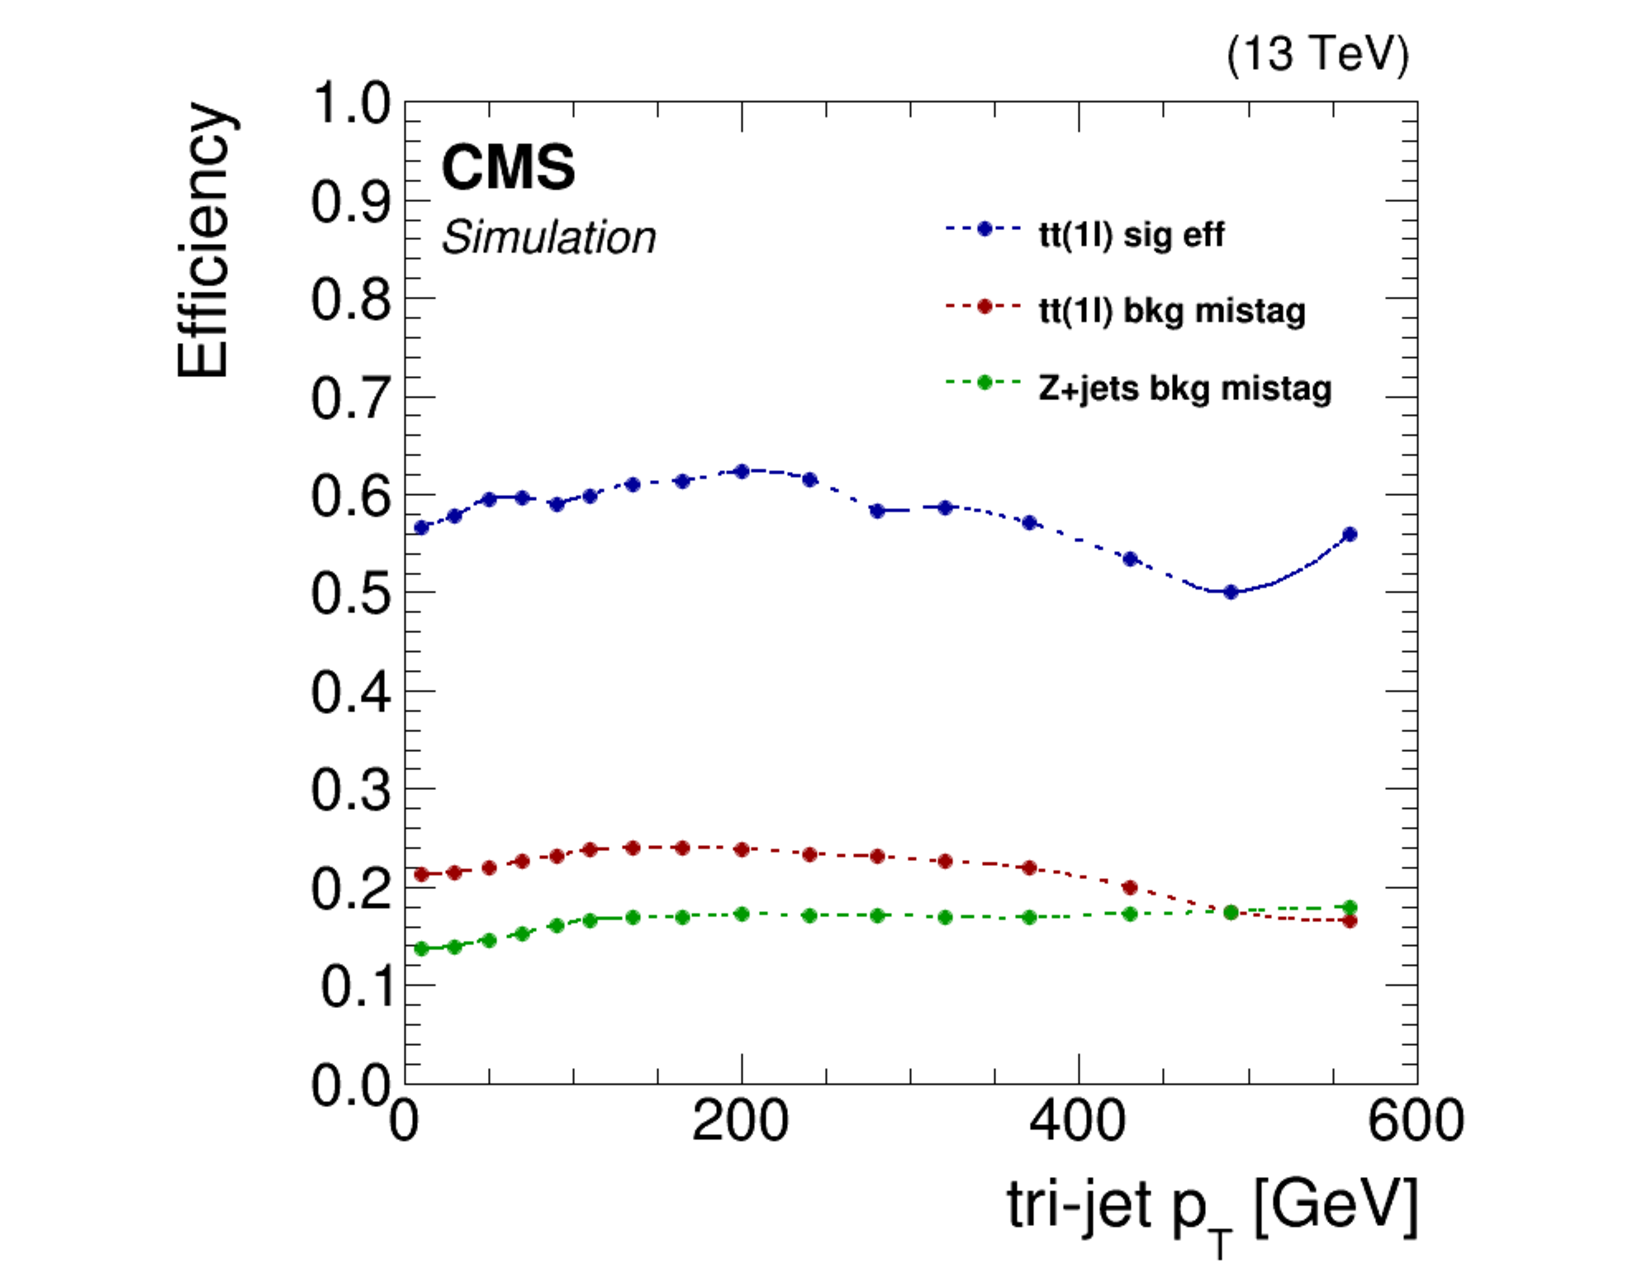
\includegraphics[width=0.48\textwidth]{figures/baseMVA+prob_bkg_effvspt.pdf}
	\caption{Resolved top tagger efficiency and mistag rates in $\ttbar(1\Lep)$ and $\Z\To\Nu\Nu$(+jets) Phys14 MC samples as a function of generator level top quark \pt\:\ and tri-jet \pt\:\ respectively}
	\label{fig:eff}
\end{figure}

The performance of the resolved top tagger was also characterized in 13\:\TeV\: data. Events for the study were selected using the HLT\_IsoMu27 trigger. The events satisfy the following offline selection criteria:

\begin{itemize}
\item exactly one muon passing ``Tight" selection with $\pt>30\:\GeV$ and $|\eta|<2.4$ 
\item $\met>100\: \GeV$
\item $M_T>40\: \GeV$
\item at least three AK4CHS jets with $\pt>30\:\GeV$ and $|\eta|<2.4$ 
\item at least two jets passing the``Medium" CSVv2+IVF WP 
\end{itemize}

The MVA output score distribution for data and MC is shown in Fig.~\ref{fig:score}. 

\begin{figure}[htbp]
	\centering
	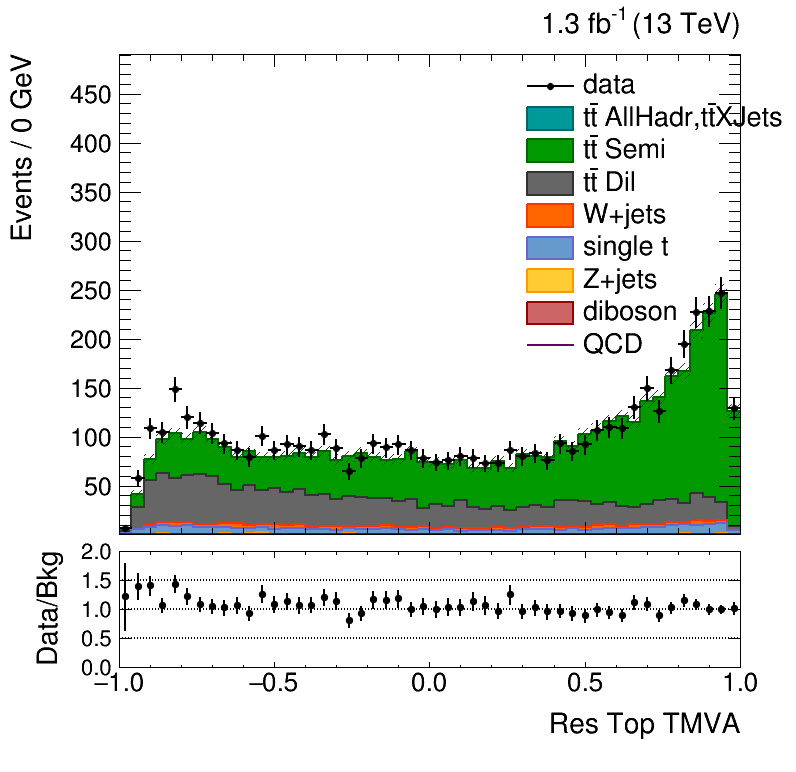
\includegraphics[width=0.48\textwidth]{figures/semilep_1tightmuo_resolved_3ormorejets_2ormorejetWPm_pfmetmore100_pfmtmore40_trigrequestonMC_qgsmearedwith8TeVrecipe_Oct302015/hResTopMVAlinear.png}
	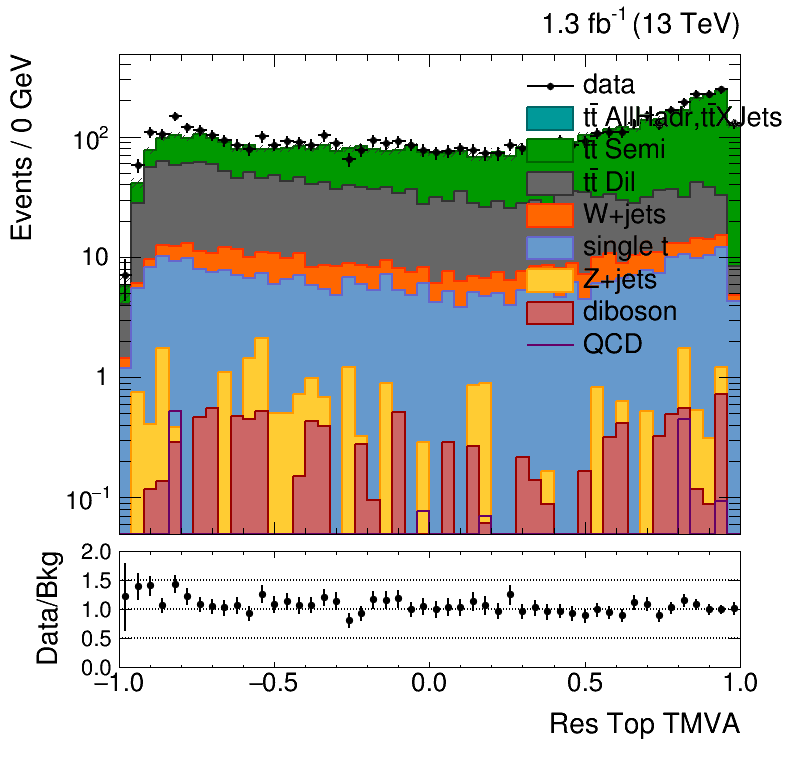
\includegraphics[width=0.48\textwidth]{figures/semilep_1tightmuo_resolved_3ormorejets_2ormorejetWPm_pfmetmore100_pfmtmore40_trigrequestonMC_qgsmearedwith8TeVrecipe_Oct302015/hResTopMVA.png}
	\caption{Resolved top tagger MVA output score distributions in data and MC in linear and log scale}
	\label{fig:score}
\end{figure}

Fair agreement is observed between data and MC, however better agreement is observed in 8\:\TeV\: studies, as described in Appendix ~\ref{app:8TeV}. The likely cause for the discrepancy at low MVA scores is due to the QGL which is currently under inverstigation (see Appendix ~\ref{app:TopTagger13TeVMore}).

In order to measure the efficiency and fake rates in data \footnote{Different efficiency/fake rate definitions used for training/characterization purposes (MC only) and scale factor measurements (data and MC comparison)}, the standard \textit{Tag and Probe} technique is employed \cite{TnP}. The semi-leptonic top candidate in the $\ttbar(1\Lep)$ event is taken to be the ``tag", while the ``probe" is the hadronically decaying top.
 The ``probe" is required to pass the aforementioned jet triplet selection. A passing ``probe" also passes the specified MVA score threshold, whereas a failing ``probe" will have an MVA output score lower than the specified threshold. The efficiency of the resolved top tagger is taken to be the number of passing ``probes" out of the total number of passing and failing ``probes".

In order to determine the yields in these categories, a simultaneous fit is performed in the orthogonal passing and failing ``probe" samples using the \textit{RooFit} framework. A $\ttbar(1\Lep)$ event can contribute either a jet triplet combination wherein each jet is matched to a generator level parton emitted from the hadronic top decay (signal) or a jet triplet combination with jets matched to underlying partons/combinatorial parton mismatch (background). Three  MC mass templates for the passing and failing ``probe" samples are constructed from:

\begin{itemize}
\item $\ttbar(1\Lep)$ signal events
\item $\ttbar(1\Lep)$ combinatorial background events
\item non-$\ttbar(1\Lep)$ background events (W/Z+jets, dibosons, single top, $\ttbar(2\Lep)$, hadronic \ttbar, \ttbar X(jets) )
\end{itemize}		 
	
The fit features six uncostrained nuisance parameters: 
\begin{itemize}
 \item signal rate in the inclusive (pass+fail) sample,
 \item combinatorial-background rate in the inclusive sample,  
 \item non-$\ttbar(1\Lep)$ background rate,
 \item signal efficiency ($\epsilon$), 
 \item combinatorial background fake rate ($FR1$) ,
 \item non-$\ttbar(1\Lep)$ background fake rate ($FR2$). 
 \end{itemize} 
 $\epsilon$, $FR1$, $FR2$ are defined respectively as the relative rates of passing ``probes" in signal, combinatorial-background, and non-$\ttbar(1\Lep)$ background.
 
 Results of the fit versus the chosen MVA score threshold is shown in Fig. \ref{fig:roofitresults13TeV}. Overall, we see good agreement, as in the 8 TeV data in appendix \ref{app:8TeV}.\\ 
  \textcolor{red}{Work on estimating the systematic uncertainties impacting the measurement.}
 
 \begin{figure}[htbp]
	\centering
	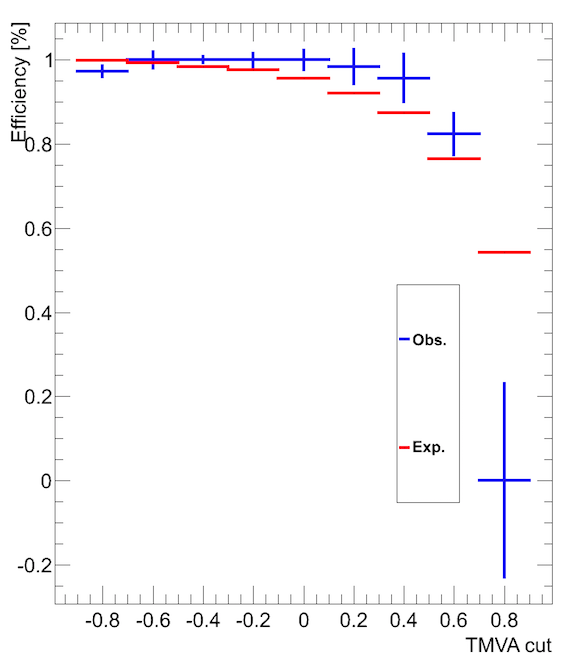
\includegraphics[width=0.48\textwidth]{figures/TOPRESOLVEDTAGGER_13TeV/c_eff.png}\\
	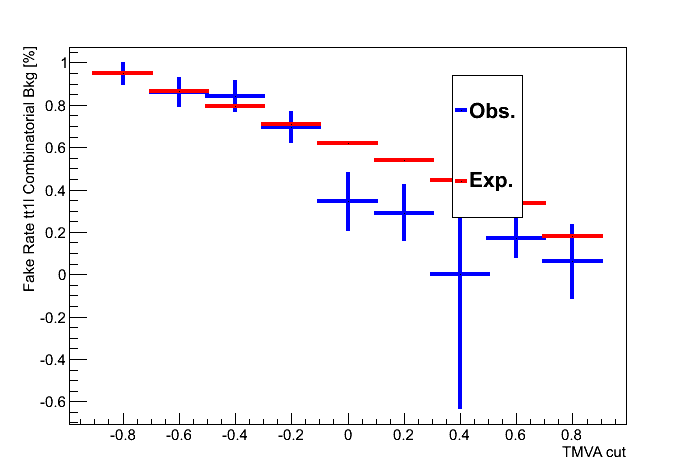
\includegraphics[width=0.48\textwidth]{figures/TOPRESOLVEDTAGGER_13TeV/c_fr1.png}
	\includegraphics[width=0.48\textwidth]{figures/TOPRESOLVEDTAGGER_13TeV/c_fr2.png}
	\caption{Signal efficiency (top),  combinatorial background fake rate (bottom left), and non-$\ttbar(1\Lep)$ background fake rate (bottom right) in data (blue) and MC (red) as function of the MVA threshold. The procedure to estimate those quantities has been described in the text.}
	\label{fig:roofitresults13TeV}
\end{figure}



















\clearpage
\subsection{Top-tagged Selection: Hadronic channel}
\label{subsec:sel_toptag_hadronic}

In the hadronic channel, there can be up to two resolved \iffalse boosted \fi top tags in the event. \iffalse This naturally leads to definitions for three signal region categories: two top tags, one top tags, and zero top tags. \fi Events are required to pass the same trigger as in the inclusive selection (Sec.~\ref{subsec:sel_incl_hadronic}) and have $\met>250\:\GeV$,  $\min_{i=1,\ldots,6}\Delta\phi\left(j_i,\met\right)>0.6$, and two jet triplet combinations with resolved top MVA score $> 0.1$. In order to have two jet triplet combinations, we require at least six AK4CHS jets in order to obtain two hadronic top candidates.

%Then, the selections for the categories are as follows:
%\begin{enumerate}
%\item \emph{Boosted, Boosted}
  %\begin{itemize}
 % \item the two leading CA15CHS jets pass boosted top tagging requirements,
 % \item at least one AK4CHS jet is $\Bot$-tagged,
  %\item $\Delta\Phi_{i=1,\ldots,6}\left(j_i,\,\met\right)>0.6$.
  %\end{itemize}
%\item \emph{Boosted, Resolved}
%  \begin{itemize}
%  \item only one of the two leading CA15CHS jets pass boosted top tagging requirements,
  %\item at least $4$ AK4CHS jets in the event,
    %\begin{itemize}
    %\item at least $1$ of which have $|\eta|<2.4$ and $\Bot$-tagged,
   % \end{itemize}
 % \item $\Delta\Phi_{i=1,\ldots,6}\left(j_i,\,\met\right)>1$.
  %\end{itemize}
%\item \emph{Resolved, Resolved}
  %\begin{itemize}
    %\item Event passes the inclusive selection of Sec.~\ref{subsec:sel_incl_hadronic}.
  %\end{itemize}
%\end{enumerate}
\iffalse To ensure the categories are exclusive, the selections are applied in the order listed above and once the event satisfies the requirments of a particular category, it is no longer considered for subsequent categories.\fi The yields in the categories are shown Table~\ref{tab:toptag_hadronic_yields}.

\begin{table}[!ht]
\centering
\begin{tabular}{|c|r|r|r|}
\hline
  Process &\iffalse \multicolumn{1}{|c|}{Boosted, Boosted} & \multicolumn{1}{|c|}{Boosted, Resolved} &\fi \multicolumn{1}{|c|}{Resolved, Resolved} \\
\hline
  \Z\To\Lep\Lep           & \iffalse $ 0.02 \pm 0.01$ & $  0.35 \pm 0.09$ &\fi $  0.52 \pm 0.12$ \\
  \Z\To\Nu\Nu             &\iffalse  $ 4.82 \pm 0.18$ & $ 58.62 \pm 1.23$ &\fi $ 72.37 \pm 1.73$ \\
  Single \Top             &\iffalse  $ 1.00 \pm 0.41$ & $ 11.42 \pm 1.40$ &\fi $ 15.88 \pm 1.61$ \\
  \Wjets                  & \iffalse $ 3.55 \pm 0.34$ & $ 36.16 \pm 2.42$ &\fi $ 38.25 \pm 3.01$ \\
  QCD                     & \iffalse $ 0.00 \pm 0.00$ & $  0.00 \pm 0.00$ &\fi $  0.00 \pm 0.00$ \\
  $\ttbar+V$              & \iffalse $ 2.61 \pm 0.19$ & $  9.63 \pm 0.37$ &\fi $  5.37 \pm 0.28$ \\
  $\ttbar(\mbox{had})$ &\iffalse $ 0.00 \pm 0.00$ & $  0.00 \pm 0.00$ &\fi $  0.00 \pm 0.00$ \\
  $\ttbar(1\Lep)$         & \iffalse $15.85 \pm 1.61$ & $127.64 \pm 4.57$ &\fi $125.35 \pm 4.53$ \\
  $\ttbar(2\Lep)$         & \iffalse $ 1.14 \pm 1.88$ & $  6.86 \pm 1.06$ & \fi$ 18.47 \pm 1.74$ \\
\hline
  SM expected             & \iffalse $29.00 \pm 1.77$ & $250.69 \pm 5.61$ &\fi $276.21 \pm 6.18$ \\
\hline
  $M_\chi=1\:\GeV$        & \iffalse $61.86 \pm 1.60$ & $247.29 \pm 3.19$ & \fi$137.42 \pm 2.38$ \\
\hline
\end{tabular}
\caption{Expected yields for $5\:\ifb$ \iffalse in each category \fi after the top-tagged selection for the hadronic channel.\textcolor{red}{Plan to pursue boosted category for Moriond}}
\label{tab:toptag_hadronic_yields}
\end{table}

\clearpage
\subsection{Top-tagged Selection: Semileptonic channel}
\label{subsec:sel_toptag_semilept}

In the semileptonic channel, there are two signal region categories: one top tag and zero top tag. The zero top tag event selection is described in Sec.~\ref{subsec:sel_incl_semilept}. For the one top tag category, events are required to pass the same trigger and lepton requirements as in the inclusive selection (Sec.~\ref{subsec:sel_incl_semilept}), as well as have $M_{T}>160\:\GeV$ and $\met>160\:\GeV$. Thus the selection requirements, not including the previously mentioned trigger and lepton requirements are:

\begin{itemize}
\item $M_{T}>160\:\GeV$,
\item$M_{T2}^W > 200\:\GeV$,
\item$\min_{i=1,2}\Delta\phi\left(j_i,\met\right)>0.8$,
\item at least one of a minimum of 3 AK4CHS jets which passes ``loose" b-tag requirements,
\item resolved top MVA score $> 0.2$.
\end{itemize}

 %The selections for the categories are as follows:
%\begin{enumerate}
%\item \emph{Boosted}
%  \begin{itemize}
%  \item the leading CA15CHS jet passes boosted top tagging requirements,
 % \item at least one AK4CHS jet is $\Bot$-tagged,
 % \item $\Delta\Phi_{i=1,\ldots,2}\left(j_i,\,\met\right)>0.6$.
 % \end{itemize}
 %\begin{enumerate}
%\item \emph{Resolved}
%  \begin{itemize}
 %   \item Event passes the inclusive selection of Sec.~\ref{subsec:sel_incl_semilept}.
 % \end{itemize}
%\end{enumerate}
%\iffalse To ensure the categories are exclusive, an event is first considered for the Boosted category and then only considered for the Resolved category if it was not already selected.\fi 

The yields in the categories are shown Table~\ref{tab:toptag_semilept_yields}.

\begin{table}[!ht]
\centering
\begin{tabular}{|c|rr|r|rr|r|}
\hline
  & \multicolumn{3}{|c|}{Boosted} & \multicolumn{3}{|c|}{Resolved} \\
  Process & \multicolumn{1}{|c}{$e$} & \multicolumn{1}{c}{$\mu$} & \multicolumn{1}{|c|}{$e+\mu$} &
            \multicolumn{1}{|c}{$e$} & \multicolumn{1}{c}{$\mu$} & \multicolumn{1}{|c|}{$e+\mu$} \\
\hline
  \Z\To\Lep\Lep          &\iffalse $ 0.02 \pm 0.01$ \fi&\iffalse $ 0.11 \pm 0.06$ \fi& \iffalse $ 0.13 \pm 0.06$   \fi&   $  0.26 \pm 0.09$ & $  0.48 \pm 0.14$ & $  0.74 \pm 0.17$ \\
  Single \Top            &\iffalse $ 1.82 \pm 0.58$\fi & \iffalse$ 2.91 \pm 0.73$ \fi&\iffalse $ 4.73 \pm 0.93$   \fi&   $  6.84 \pm 1.11$ & $ 11.37 \pm 1.43$ & $ 18.22 \pm 1.81$ \\
  \Wjets                 &\iffalse $ 2.92 \pm 0.68$ \fi&\iffalse $ 4.71 \pm 1.22$ \fi& \iffalse$ 7.63 \pm 1.40$   \fi&   $  8.96 \pm 1.43$ & $ 13.93 \pm 2.26$ & $ 22.89 \pm 2.67$ \\
  $\ttbar+V$             & \iffalse$ 2.51 \pm 0.19$ \fi&\iffalse $ 2.90 \pm 0.20$ \fi&\iffalse $ 5.40 \pm 0.28$   \fi&   $  3.07 \pm 0.21$ & $  3.86 \pm 0.23$ & $  6.93 \pm 0.31$ \\
  $\ttbar(\mbox{had})$   &\iffalse $ 0.00 \pm 0.00$\fi & \iffalse$ 0.00 \pm 0.00$ \fi&\iffalse $ 0.00 \pm 0.00$   \fi&   $  0.00 \pm 0.00$ & $  0.00 \pm 0.00$ & $  0.00 \pm 0.00$ \\
  $\ttbar(1\Lep)$        & \iffalse$24.51 \pm 2.00$\fi &\iffalse $24.68 \pm 2.01$ \fi& \iffalse$49.19 \pm 2.84$   \fi&   $ 71.58 \pm 3.42$ & $ 89.72 \pm 3.83$ & $161.31 \pm 5.13$ \\
  $\ttbar(2\Lep)$        & \iffalse$ 2.45 \pm 0.63$\fi & \iffalse$ 2.78 \pm 0.67$ \fi& \iffalse$ 5.23 \pm 0.92$   \fi&   $  1.96 \pm 0.57$ & $  2.12 \pm 0.59$ & $  4.09 \pm 0.82$ \\
\hline
  SM expected            & \iffalse$34.23 \pm 2.29$\fi & \iffalse$38.08 \pm 2.56$ \fi& \iffalse$72.31 \pm 3.43$   \fi&   $ 92.68 \pm 3.92$ & $121.49 \pm 4.72$ & $214.17 \pm 6.13$ \\
\hline
  $M_\chi=1\:\GeV$       & \iffalse$28.88 \pm 1.09$\fi & \iffalse$35.91 \pm 1.22$\fi & \iffalse$64.78 \pm 1.63$   \fi&   $ 54.05 \pm 1.49$ & $ 67.33 \pm 1.66$ & $121.38 \pm 2.23$ \\
\hline
\end{tabular}
\caption{Expected yields for $5\:\ifb$ in each category after the top-tagged selection for the semileptonic channel.}
\label{tab:toptag_semilept_yields}
\end{table}


%\clearpage

\section{Background Estimation}
\label{sec:background}

The general approach for background estimation is to derive data/MC scale factor corrections from background enriched control regions (CR) and apply these to the MC predictions for the signal region (SR). Formally, for a particular background process,
\begin{equation}
  N_{\mbox{\scriptsize{SR}}}^{\mbox{\scriptsize{predict}}} = N_{\mbox{\scriptsize{SR}}}^{\mbox{\scriptsize{MC}}}
\left(\frac{N_{\mbox{\scriptsize{CR}}}^{\mbox{\scriptsize{data}}}}{N_{\mbox{\scriptsize{CR}}}^{\mbox{\scriptsize{MC}}}}\right),
\end{equation}
where $N_{\mbox{\scriptsize{SR}}}^{\mbox{\scriptsize{predict}}}$ is the signal region prediction for the background of interest, $N_{\mbox{\scriptsize{SR}}}^{\mbox{\scriptsize{MC}}}$ is the MC yield in the signal region, and $N_{\mbox{\scriptsize{CR}}}^{\mbox{\scriptsize{data}}}$ and $N_{\mbox{\scriptsize{CR}}}^{\mbox{\scriptsize{MC}}}$ are the yields in the control region for data and MC respectively. For a cut-and-count analysis, the formula states the MC yields in the SR are corrected by the ratio of data-to-MC yields in the CR. For a shape analysis, the formula implies bin-by-bin correction factors in the variable used for signal extraction (i.e. $\met$).

To handle signal contamination in the control regions and as well as backgrounds that contribute substantially to multiple control regions, the signal extraction and scale factor derivation will be performed simultaneously across all signal and control regions. (This is not yet done for this note.)

\subsection{Backgrounds: Hadronic channel}
\label{subsec:bkg_hadronic}

The main backgrounds in this channel are semileptonic $\ttbar$, $\Wjets$, and $\Z(\Nu\Nu)+$jets, and control regions enriched in these backgrounds are defined in the following. Also, a control region for QCD is defined to validate that the background is expected to be small.

\subsubsection{Control region for \texorpdfstring{$\ttbar$}{ttbar}}
\label{subsubsec:bkg_hadronic_ttbar}

A control region enriched in semileptonic $\ttbar$ can be obtained by requiring exactly one ``Tight'' electron or muon with $M_T<160\:\GeV$, while keeping all other selection requirements.\iffalse For the categories with boosted top tags, the subjet $\Bot$-tag requirements are dropped.To obtain a $\met$ template, the four-momentum of the lepton is removed and it is this lepton subtracted $\met$ quantity that must be greater than $250\:\GeV$.\fi From the studies shown in Appendix ~\ref{app:CR}, we determine that removal of the lepton four-momentum from the $\met$ in this control region isn't necessary in order to model the $\met$ distribution in the signal region. The yields are listed in Table~\ref{tab:hadronic_bkg_tt1l_yields}. The \iffalse lepton subtracted \fi $\met$ distributions in the control region for the inclusive selection is shown in Fig.~\ref{fig:incl_hadronic_1l_fmet} for both the electron and muon selection. 

\begin{table}[!ht]
\centering
\begin{tabular}{|c|r|r|}
\hline
  Process & \multicolumn{1}{|c|}{Electron Channel} & \multicolumn{1}{|c|}{Muon Channel} \\
\hline
  Diboson         & $   1.09 \pm  0.33$ & $  0.97 \pm  0.27$ \\
  \Zjets            & $ 0.58 \pm  0.22$ &$4.07 \pm  1.23$ \\
  Single \Top    & $ 52.12 \pm 1.48$ &  $57.99 \pm  1.51$ \\
  \Wjets            & $   34.97 \pm  1.10$ & $  46.53 \pm  1.53$ \\
  $\ttbar$   & $   618.07 \pm  3.17$ & $  710.05 \pm  3.30$ \\
  QCD        & $ 0.00 \pm 0.00$ & $0.00\pm  0.00$ \\
\hline
SM expected     & $706.83 \pm 3.69$ & $819.61 \pm 4.14$ \\
 \hline
  Observed        & $719.00 \pm 0.00$ & $883.00 \pm 0.00$ \\
\hline
  $M_\chi=1\:\GeV\:, M_\phi=10\:\GeV\:$       & $  1.30 \pm  0.12$ &  $2.30  \pm  0.16$ \\
\hline
\end{tabular}
\caption{Expected and observed yields for $1.3\:\ifb$ in the $\ttbar$ control region for the hadronic channel.}
\label{tab:hadronic_bkg_tt1l_yields}
\end{table}

\begin{figure}[htbp]
  \centering
  \includegraphics[width=0.48\textwidth]{figures/hMETlinear_CRttbar_el.png}
  \includegraphics[width=0.48\textwidth]{figures/hMETlinear_CRttbar_mu.png}
    \caption{The $\met$ distribution in the $\ttbar$ control region with electron (left) and muon (right) selection for the hadronic channel.}
  \label{fig:incl_hadronic_1l_fmet}
\end{figure}

\clearpage
\subsubsection{Control region for \texorpdfstring{$V+$jets}{Vjets}}
\label{subsubsec:bkg_hadronic_vjets}

By requiring no $\Bot$-tagged jets in the event and keeping all other cuts the same, a sample enriched in $\Wjets$ and $\Z(\Nu\Nu)+$jets can be obtained. From the studies shown in Appendix ~\ref{app:CR}, we determine that removal of the lepton four-momentum from the $\met$ in the $V+$jets control region isn't necessary in order to model the $\met$ distribution in the signal region. \iffalse For the categories with boosted top tags, the subjet $\Bot$-tag requirements are dropped.\fi  The yields are listed in Table~\ref{tab:hadronic_bkg_vjets_yields}. The $\met$ distributions in the control region for the inclusive selection is shown in Fig.~\ref{fig:incl_hadronic_0b_met}.

\begin{table}[!ht]
\centering
\begin{tabular}{|c|r|}
\hline
  Process & \\
\hline
  Diboson         & $ 33.10 \pm 1.89 $ \\
  \Zjets            & $681.22 \pm 3.91$ \\
  Single \Top    & $21.65 \pm 0.95 $ \\
  \Wjets            & $ 1341.57 \pm 11.81 $ \\
  $\ttbar$   & $    221.19 \pm 1.94$ \\
  QCD        & $ 19.54 \pm 2.96$ \\
\hline
SM expected     & $  2318.28 \pm 13.11$\\
 \hline
  Observed        & $2380.00 \pm 0.00$ \\
\hline
  $M_\chi=1\:\GeV\:, M_\phi=10\:\GeV\:$       & $ 2.76 \pm 0.18$ \\
\hline
\end{tabular}
\caption{Expected yields for $1.3\:\ifb$ in the $V+$jets control region for the hadronic channel.}
\label{tab:hadronic_bkg_vjets_yields}
\end{table}

\begin{figure}[htbp]
  \centering
  \includegraphics[width=0.48\textwidth]{figures/hMETlinear_CRvjets_0b.png}
  \caption{The $\met$ distribution in the $V+$jets control region for the hadronic channel.}
  \label{fig:incl_hadronic_0b_met}
\end{figure}

\subsubsection{Control region for \texorpdfstring{$\Wjets$}{Wjets}}
\label{subsubsec:bkg_hadronic_wjets}

A control region enriched in $\Wjets$ can be obtained by requiring a ``Tight'' electron or muon and no $\Bot$-tagged jets, while keeping all other selection requirements. \iffalse For the categories with boosted top tags, the subjet $\Bot$-tag requirements are dropped. \fi To obtain a $\met$ template, we do not remove the lepton four-momentum and require that this $\met$ quantity that must be greater than $250\:\GeV$. Studies that support retaining the lepton \pt\: are detailed in Appendix~\ref{app:CR}.The expected and observed yields are listed in Table~\ref{tab:hadronic_bkg_vjets_yields}. The \iffalse lepton subtracted \fi $\met$ distributions in the control region for the inclusive selection is shown in Fig.~\ref{fig:incl_hadronic_1l0b_fmet} for both the electron and muon selection.

\begin{table}[!ht]
\centering
\begin{tabular}{|c|r|r|}
\hline
  Process & \multicolumn{1}{|c|}{Electron Channel} & \multicolumn{1}{|c|}{Muon Channel} \\
\hline
  Diboson         & $  000000$ & $17.72 \pm 1.48$ \\
  \Zjets            & $20.61 \pm1.98$ &  $24.65 \pm 2.07$ \\
  Single \Top    & $ 23.65 \pm 0.98$ &  $30.23 \pm 1.13$ \\
  \Wjets            & $ 770.08 \pm 6.72$ & $  886.25 \pm 7.32$ \\
  $\ttbar$   & $   253.06 \pm 2.03$ & $  313.48 \pm 2.30$ \\
  QCD        & $ 3.13 \pm 1.32$ & $0.64 \pm 0.60$ \\
\hline
SM expected     & $1088.29 \pm 7.62$ & $1272.98 \pm 8.19$ \\
 \hline
  Observed        & $939.00 \pm 0.00$ & $1167.00 \pm 0.00$ \\
\hline
  $M_\chi=1\:\GeV\:, M_\phi=10\:\GeV\:$       & $  0.94 \pm  0.10$ &  $1.19  \pm  0.12$ \\
\hline
\end{tabular}
\caption{Expected and observed yields for $1.3\:\ifb$ in the $\Wjets$ control region for the hadronic channel.}
\label{tab:hadronic_bkg_wjets_yields}
\end{table}

\begin{figure}[htbp]
  \centering
  \includegraphics[width=0.48\textwidth]{figures/hMETlinear_CRwjets_el.png}
  \includegraphics[width=0.48\textwidth]{figures/hMETlinear_CRwjets_mu.png}
  \caption{The $\met$ distribution in the $\Wjets$ control region for the hadronic channel for electron (left) and muon (right) selection.}
  \label{fig:incl_hadronic_1l0b_fmet}
\end{figure}


%2j/0b
%  *     Z+jets    954.88 +/-   6.92
%  *   single t    332.13 +/-   6.67
%  *     W+jets  42025.86 +/- 136.36
%  * t#bar{t}+V      0.75 +/-   0.10
%  * t#bar{t}(had)      0.16 +/-   0.16
%  * t#bar{t}(2l)    122.08 +/-   4.47
%  * t#bar{t}(1l)    639.34 +/-  10.22
%  ============
%     total bkg  44075.21 +/- 137.16
%      DM 1 GeV      3.41 +/-   0.37

%2j/2b
%  *     Z+jets      2.46 +/-   0.31
%  *   single t     31.57 +/-   2.11
%  *     W+jets     77.21 +/-   5.23
%  * t#bar{t}+V      0.11 +/-   0.04
%  * t#bar{t}(had)      0.00 +/-   0.00
%  * t#bar{t}(2l)     26.80 +/-   2.09
%  * t#bar{t}(1l)     71.75 +/-   3.42
%  ============
%     total bkg    209.91 +/-   6.93
%      DM 1 GeV      0.90 +/-   0.19


%2j/1b
%  *     Z+jets     78.01 +/-   1.91
%  *   single t    293.13 +/-   6.49
%  *     W+jets   3057.11 +/-  35.02
%  * t#bar{t}+V      1.07 +/-   0.12
%  * t#bar{t}(had)      0.00 +/-   0.00
%  * t#bar{t}(2l)    190.56 +/-   5.58
%  * t#bar{t}(1l)    700.46 +/-  10.70
%  ============
%     total bkg   4320.34 +/-  37.65
%      DM 1 GeV      6.13 +/-   0.50

\clearpage
\subsubsection{Control region for \texorpdfstring{$\Zjets$}{Zjets}}
\label{subsubsec:bkg_hadronic_zjets}

A control region enriched in $\Zjets$ can be obtained by requiring a pair of ``Tight'' electrons or muons, with dilepton mass between $60\:\GeV$ and $120\:\GeV$, and no $\Bot$-tagged jets, while keeping all other selection requirements. The agreement between the $\met$ distribution in the $\Zjets$ control and signal regions shown in Appendix~\ref{app:CR} validate the following extracted $\met$ distribution. \iffalse For the categories with boosted top tags, the subjet $\Bot$-tag requirements are dropped. \fi To obtain a $\met$ template for $\Z\To\Nu\Nu$, the four-momentum of the dilepton system is removed and it is the dilepton subtracted $\met$ that must be greater than $250\:\GeV$. The yields are listed in Table~\ref{tab:hadronic_bkg_zjets_yields}. The lepton subtracted $\met$ distributions in the control region for the inclusive selection is shown in Fig.~\ref{fig:incl_hadronic_2l0b_fmet}.

\begin{table}[!ht]
\centering
\begin{tabular}{|c|r|r|}
\hline
  Process & \multicolumn{1}{|c|}{$ee$} & \multicolumn{1}{|c|}{$\mu\mu$} \\
\hline
  Diboson         & $  3.70 \pm 0.47$ & $4.15 \pm 0.46$ \\
  \Zjets            & $134.70 \pm 4.50$ &  $213.82 \pm 5.85$ \\
  Single \Top    & $ 0.83 \pm 0.18$ &  $0.79 \pm 0.17$ \\
  \Wjets            & $ 0.35 \pm 0.12$ & $  0.21 \pm 0.11$ \\
  $\ttbar$   & $   10.52 \pm 0.41$ & $   16.72 \pm 0.53$ \\
  QCD        & $0.07 \pm 0.07$ & $ 1.63 \pm 1.08$ \\
\hline
SM expected     & $150.17 \pm 4.55$ & $237.33 \pm 5.99$ \\
 \hline
  Observed        & $170.00 \pm 0.00$ & $274.00 \pm 0.00$ \\
\hline
  $M_\chi=1\:\GeV\:, M_\phi=10\:\GeV\:$       & $  0.00 \pm 0.00$ &  $0.02 \pm 0.02$ \\
\hline
\end{tabular}

\caption{Expected yields for $1.3\:\ifb$ in the $\Zjets$ control region with dileptons for the hadronic channel.}
\label{tab:hadronic_bkg_zjets_yields}
\end{table}

\begin{figure}[htbp]
  \centering
  \includegraphics[width=0.48\textwidth]{figures/hMETNoLepLinear_CRzjets_el.png}
  \includegraphics[width=0.48\textwidth]{figures//hMETNoLepLinear_CRzjets_mu.png}
  \caption{The $\met$ distribution in the $\Zjets$ control region with dileptons for the hadronic channel with the double electron (left) and double muon (right) selection.}
  \label{fig:incl_hadronic_2l0b_fmet}
\end{figure}

%2j/0b
%  *     Z+jets   3240.14 +/-  12.37
%  *   single t      3.64 +/-   0.82
%  *     W+jets      0.15 +/-   0.09
%  *   t#bar{t}     14.71 +/-   1.55
%  * t#bar{t}+V      0.04 +/-   0.02
%  ============
%     total bkg   3258.69 +/-  12.49
%      DM 1 GeV      0.16 +/-   0.08

%2j/2b
%  *     Z+jets      8.49 +/-   0.58
%  *   single t      1.63 +/-   0.54
%  *     W+jets      0.00 +/-   0.00
%  *   t#bar{t}      0.82 +/-   0.37
%  * t#bar{t}+V      0.01 +/-   0.01
%  ============
%     total bkg     10.95 +/-   0.88
%      DM 1 GeV      0.04 +/-   0.04

%2j/1b
%  *     Z+jets    264.17 +/-   3.39
%  *   single t      6.72 +/-   1.11
%  *     W+jets      0.00 +/-   0.00
%  *   t#bar{t}     14.55 +/-   1.54
%  * t#bar{t}+V      0.13 +/-   0.04
%  ============
%     total bkg    285.56 +/-   3.88
%      DM 1 GeV      0.29 +/-   0.11

Another way to model the $\met$ distribution for $\Z(\Nu\Nu)+$jets is to use $\gamma+$jets events. The $\gamma+$jets yields are much higher than for $\Z(\Lep\Lep)+$jets, however theoretical corrections must be applied to the photon $\pt$ spectrum to make it more $\Z$-like, and this introduces some systematic uncertainty. The selection for the control region takes events passing the HLT\_Photon155 trigger, requires the leading photon in the event to have $\pt>100\:\GeV$, $|\eta|<2.5$ while excluding the barrel-endcap transition region ($1.4442<|\eta_{\mbox{\scriptsize{SC}}}|>1.556$), and to pass the ``Medium'' WP. All other signal region cuts are applied, including $\Bot$-tagging requirements. To obtain a $\met$ template for $\Z\To\Nu\Nu$, the four-momentum of the photon is removed and it is the photon subtracted $\met$ that must be greater than $200\:\GeV$. The yields are listed in Table~\ref{tab:hadronic_bkg_pho_yields}. The lepton subtracted $\met$ distributions in the control region for the inclusive selection is shown in Fig.~\ref{fig:incl_hadronic_pho_fmet}.

\begin{table}[!ht]
\centering
\begin{tabular}{|c|r|}
\hline
  Process & \\
\hline
  $\gamma+$jets  & $245.11 \pm 6.78$ \\
  QCD                   & $27.20 \pm 2.90$  \\
\hline
SM expected     & $272.30 \pm 7.38$ \\
 \hline
  Observed        & $295.00 $ \\
\hline
  $M_\chi=1\:\GeV\:, M_\phi=10\:\GeV\:$       & $  0.00 \pm 0.00$ \\
\hline
\end{tabular}

\caption{Expected yields for $1.3\:\ifb$ in the $\Zjets$ control region with photons for the hadronic channel.}
\label{tab:hadronic_bkg_pho_yields}
\end{table}
\begin{figure}[htbp]
  \centering
  \includegraphics[width=0.48\textwidth]{figures/hPFMETnopholinear_CRzjets.png}
  \caption{The $\met$ distribution in the $\Zjets$ control region with photons for the hadronic channel.}
  \label{fig:incl_hadronic_pho_fmet}
\end{figure}

\subsubsection{Control region for QCD}
\label{subsubsec:bkg_hadronic_qcd}

To obtain a control region enriched in QCD, consider events with no $\Bot$-tagged jets and $\min_{i=1,\ldots,6}\Delta\phi\left(j_i,\,\met\right)<1$. Typically, MC samples for QCD are very statistically limited so the purpose of the control region is to verify that QCD is negligible by looking at the level of data/MC agreement as $\min_{i=1,\ldots,6}\Delta\phi\left(j_i,\,\met\right)$ approaches $1$. If the agreement is good, then it can be concluded that the QCD contribution is negligible. The $\Delta\phi$ distribution in this region is shown in Fig.~\ref{fig:incl_hadronic_qcd_dphijetmet}.

\begin{figure}[htbp]
  \centering
  \includegraphics[width=0.48\textwidth]{figures/hadronic-incl-qcd-dphijetmet.pdf}
  \includegraphics[width=0.48\textwidth]{figures/hadronic-incl-qcd-dphijetmetlog.pdf}
  \caption{The $\min_{i=1,\ldots,6}\Delta\phi\left(j_i,\,\met\right)$ distribution in the QCD control region for the hadronic channel.}
  \label{fig:incl_hadronic_qcd_dphijetmet}
\end{figure}

\subsection{Backgrounds: Semileptonic channel}
\label{subsec:bkg_semilept}

Control regions for the two major backgrounds, dileptonic $\ttbar$ and $\Wjets$, are described in the following.

\subsubsection{Control region for \texorpdfstring{$\ttbar$}{ttbar}}
\label{subsubsec:bkg_semilept_ttbar}

A control region enriched in dileptonic $\ttbar$ can be obtained by requiring a $ee$, $e\mu$, and $\mu\mu$ dilepton pairs where each lepton passes ``Tight'' selection. The four-momentum of the trailing lepton is subtracted from the event to construct the $\met$ template, and is used to compute all $\met$-related variables: $M_T, M_{T2}^W, \min_{i=1,2}\Delta\phi\left(j_i,\,\met\right)$. All other selection cuts for the semileptonic channel are applied accordingly. The yields are listed in Table~\ref{tab:semilept_bkg_tt2l_yields}. The lepton subtracted $\met$ distributions in the control region for the inclusive selection is shown in Fig.~\ref{fig:incl_semilept_2l_fmet}.

\begin{table}[!ht]
\centering
\begin{tabular}{|c|rr|rr|rr|}
\hline
  Process & \multicolumn{2}{|c|}{Inclusive} & \iffalse \multicolumn{2}{|c|}{Boosted} &\fi \multicolumn{2}{|c|}{Resolved} \\
          & $e$ & $\mu$                     & \iffalse$e$ & $\mu$                   &\fi $e$ & $\mu$ \\
\hline
  \Z\To\Lep\Lep          & $  0.50 \pm 0.13$ & $  0.62 \pm 0.12$  &\iffalse $ 0.19 \pm 0.09$ & $ 0.12 \pm 0.02$  &\fi $  0.38 \pm 0.11$ & $  0.52 \pm 0.11$ \\
  Single \Top            & $ 11.80 \pm 1.46$ & $ 13.35 \pm 1.56$  &\iffalse $ 1.09 \pm 0.45$ & $ 1.64 \pm 0.55$  & \fi$ 11.25 \pm 1.43$ & $ 12.26 \pm 1.49$ \\
  \Wjets                 & $  0.03 \pm 0.03$ & $  0.03 \pm 0.03$  & \iffalse$ 0.03 \pm 0.03$ & $ 0.00 \pm 0.00$  & \fi$  0.03 \pm 0.03$ & $  0.03 \pm 0.03$ \\
  $\ttbar+V$             & $  1.86 \pm 0.16$ & $  1.86 \pm 0.03$  & \iffalse$ 0.62 \pm 0.09$ & $ 0.55 \pm 0.09$  & \fi$  1.52 \pm 0.15$ & $  1.51 \pm 0.15$ \\
  $\ttbar(\mbox{had})$   & $  0.00 \pm 0.00$ & $  0.00 \pm 0.00$  &\iffalse $ 0.00 \pm 0.00$ & $ 0.00 \pm 0.00$  & \fi$  0.00 \pm 0.00$ & $  0.00 \pm 0.00$ \\
  $\ttbar(1\Lep)$        & $  0.16 \pm 0.16$ & $  0.00 \pm 0.00$  &\iffalse $ 0.00 \pm 0.00$ & $ 0.00 \pm 0.00$  & \fi$  0.16 \pm 0.16$ & $  0.00 \pm 0.00$ \\
  $\ttbar(2\Lep)$        & $107.05 \pm 4.18$ & $112.77 \pm 4.29$  &\iffalse $13.73 \pm 1.50$ & $14.71 \pm 1.55$  &\fi $102.80 \pm 4.10$ & $108.35 \pm 4.21$ \\
\hline
  SM expected            & $121.39 \pm 4.44$ & $128.63 \pm 4.57$  &\iffalse $15.65 \pm 1.57$ & $17.01 \pm 1.65$  & \fi$116.13 \pm 4.35$ & $122.68 \pm 4.47$ \\
\hline
  $M_\chi=1\:\GeV$       & $  4.94 \pm 0.45$ & $  6.38 \pm 0.51$  &\iffalse $ 0.16 \pm 0.08$ & $ 0.53 \pm 0.15$  &\fi $  4.81 \pm 0.44$ & $  6.21 \pm 0.51$ \\
\hline
\end{tabular}
\caption{Expected yields for $5\:\ifb$ in the $\ttbar$ control region for the semileptonic channel.}
\label{tab:semilept_bkg_tt2l_yields}
\end{table}

\begin{figure}[htbp]
  \centering
  \includegraphics[width=0.48\textwidth]{figures/semilept-incl-2l-fmet_l.pdf}
  \includegraphics[width=0.48\textwidth]{figures/semilept-incl-2l-fmetlog_l.pdf}
  \caption{The $\met$ distribution in the $\ttbar$ control region for the semileptonic channel.}
  \label{fig:incl_semilept_2l_fmet}
\end{figure}

\subsubsection{Control region for \texorpdfstring{$\Wjets$}{Wjets}}
\label{subsubsec:bkg_semilept_wjets}

By requiring no $\Bot$-tagged jets in the event and keeping all other cuts the same, a sample enriched in $\Wjets$  can be obtained. \iffalse For the categories with boosted top tags, the subjet $\Bot$-tag requirements are dropped. \fi The yields are listed in Table~\ref{tab:semilept_bkg_wjets_yields}. The $\met$ distributions in the control region for the inclusive selection is shown in Fig.~\ref{fig:incl_semilept_0b_met}.

\begin{table}[!ht]
\centering
\begin{tabular}{|c|rr|rr|rr|}
\hline
  Process & \multicolumn{2}{|c|}{Inclusive} &\iffalse \multicolumn{2}{|c|}{Boosted} &\fi \multicolumn{2}{|c|}{Resolved} \\
          & $e$ & $\mu$                     & \iffalse$e$ & $\mu$                   &\fi $e$ & $\mu$ \\
\hline
  \Z\To\Lep\Lep          & $ 0.40 \pm 0.26$ & $ 0.51 \pm 0.11$  &\iffalse $ 0.12 \pm 0.03$ & $ 0.53 \pm 0.14$  & \fi$ 0.38 \pm 0.26$ & $ 0.43 \pm 0.11$ \\
  Single \Top            & $ 1.33 \pm 0.49$ & $ 1.52 \pm 0.52$  & \iffalse$ 0.55 \pm 0.32$ & $ 0.78 \pm 0.37$  &\fi $ 1.15 \pm 0.45$ & $ 1.28 \pm 0.48$ \\
  \Wjets                 & $46.58 \pm 4.47$ & $57.74 \pm 5.59$  & \iffalse$20.18 \pm 2.60$ & $24.80 \pm 2.98$  &\fi $40.75 \pm 4.33$ & $50.33 \pm 5.44$ \\
  $\ttbar+V$             & $ 0.44 \pm 0.08$ & $ 0.64 \pm 0.09$  & \iffalse$ 0.56 \pm 0.09$ & $ 0.67 \pm 0.10$  & \fi$ 0.31 \pm 0.07$ & $ 0.51 \pm 0.08$ \\
  $\ttbar(\mbox{had})$   & $ 0.00 \pm 0.00$ & $ 0.00 \pm 0.00$  & \iffalse$ 0.00 \pm 0.00$ & $ 0.00 \pm 0.00$  & \fi$ 0.00 \pm 0.00$ & $ 0.00 \pm 0.00$ \\
  $\ttbar(1\Lep)$        & $ 0.16 \pm 0.16$ & $ 0.16 \pm 0.16$  & \iffalse$ 0.33 \pm 0.23$ & $ 1.14 \pm 0.43$  & \fi$ 8.83 \pm 1.20$ & $10.79 \pm 1.33$ \\
  $\ttbar(2\Lep)$        & $ 9.97 \pm 1.28$ & $12.09 \pm 1.41$  &\iffalse $ 8.17 \pm 1.16$ & $ 9.15 \pm 1.22$  & \fi$ 0.16 \pm 0.16$ & $ 0.16 \pm 0.16$ \\
\hline
  SM expected            & $58.88 \pm 4.69$ & $72.67 \pm 5.79$  &\iffalse $29.89 \pm 2.87$ & $37.07 \pm 3.27$  & \fi$51.57 \pm 4.53$ & $63.50 \pm 5.63$ \\
\hline
  $M_\chi=1\:\GeV$       & $10.24 \pm 0.65$ & $12.01 \pm 0.70$  & \iffalse$ 6.62 \pm 0.52$ & $ 8.35 \pm 0.59$  &\fi $ 7.69 \pm 0.56$ & $ 8.43 \pm 0.59$ \\
\hline
\end{tabular}
\caption{Expected yields for $5\:\ifb$ in the $\Wjets$ control region for the semileptonic channel.}
\label{tab:semilept_bkg_wjets_yields}
\end{table}

\begin{figure}[htbp]
  \centering
  \includegraphics[width=0.48\textwidth]{figures/semilept-incl-0b-met_l.pdf}
  \includegraphics[width=0.48\textwidth]{figures/semilept-incl-0b-metlog_l.pdf}
  \caption{The $\met$ distribution in the $\Wjets$ control region for the semileptonic channel.}
  \label{fig:incl_semilept_0b_met}
\end{figure}


\clearpage

\section{Systematic Uncertainties}
\label{sec:systematics}

For backgrounds estimated by applying data/MC corrections derived from the control regions, the systematic uncertainty comes from the statistical uncertainty in the control regions as well as any systematic difference in extrapolating from the control region to the signal region (e.g. modeling $\Zjets$ with $\gamma+$jets). For the signal and backgrounds estimated purely with MC, the main sources of systematic uncertainties are:

\begin{itemize}
\item Parton distribution function: evalulated by computing the change in yiels or shape from the error sets provided by the PDF set.
\item Missing higher order terms: evaluated by the usual procedure of varying the QCD factorization and renormalization scale together by a factor of $0.5$ and by a factor of $2$, and compute the change in yields or shape.
\item Efficiencies: uncertainty on the various data/MC efficiency scale factors used to correct the MC:
  \begin{itemize}
  \item trigger
  \item lepton selection
  \item $\Bot$-tagging
  \item top-tagging (category migration effects)
  \end{itemize}
\item $\met$ scale and resolution
\item Jet energy scale and resolution
\item Luminosity
\end{itemize}

\clearpage

\section{Results}
\label{sec:results}

Expected upper limits at $95\%$ confidence level on the cross section ratio with respect to $M_*=100\:\GeV$ are computed with the COMBINE tool. For a given $M_\chi$, the EFT is only charaterized by $M_*$, and therefore a lower limit on the interaction mass scale can also be computed. We are also running over simplified models, however the text below is with respect to EFT models. Systematic uncertainties are not yet considered.

\subsection{Cut and count analysis}
\label{subsec:cutcount}

An uncategorized cut-and-count analysis is performed by applying an additional cut of $\met>320\:\GeV$ to define the signal region. The upper limits on the cross section ratio are shown in Fig.~\ref{fig:rlimits_count}. The hadronic and semileptonic channels both have roughly the same sensitivity. By combining the channels, the limits improve by about $30\%$. The limits on the cross section ratio and $M_*$ are shown in Fig.~\ref{fig:rlimits_count} and Fig.~\ref{fig:mstarlimits_count}, respectively.

\begin{figure}[htbp]
\begin{center}
  \subfigure[Hadronic]{\label{subfig:hadronic_count}\includegraphics[width=0.32\textwidth]{figures/rLimit_hadronic_incl_count.pdf}}
  \subfigure[Semileptonic]{\label{subfig:semilept_count}\includegraphics[width=0.32\textwidth]{figures/rLimit_semilept_incl_count.pdf}}
  \subfigure[Combined]{\label{subfig:combined_count}\includegraphics[width=0.32\textwidth]{figures/rLimit_incl_count.pdf}}
  \caption{Expected upper limits on the cross section ratio relative to $M_*=100\:\GeV$ for the inclusive selections: \subref{subfig:hadronic_count} hadronic channel, \subref{subfig:semilept_count} semileptonic channel, \subref{subfig:combined_count} combination of both channels.}
  \label{fig:rlimits_count}
\end{center}
\end{figure}

\begin{table}[!ht]
\centering
\begin{tabular}{|r|c|c|c|}
\hline
  $M_\chi$ $(\GeV)$ & Median & $\left[-1\sigma\, +1\sigma\right]$ & $\left[-2\sigma\, +2\sigma\right]$ \\
\hline
  $1$               & $0.1030$ & $\left[0.0730\, 0.1461\right]$ & $\left[0.0543\, 0.1990\right]$ \\
  $10$              & $0.1050$ & $\left[0.0744\, 0.1498\right]$ & $\left[0.0554\, 0.2047\right]$ \\
  $50$              & $0.1021$ & $\left[0.0723\, 0.1448\right]$ & $\left[0.0538\, 0.1971\right]$ \\
  $100$             & $0.1167$ & $\left[0.0827\, 0.1665\right]$ & $\left[0.0615\, 0.2261\right]$ \\
  $200$             & $0.1548$ & $\left[0.1097\, 0.2196\right]$ & $\left[0.0813\, 0.3010\right]$ \\
  $600$             & $0.6973$ & $\left[0.4960\, 0.9891\right]$ & $\left[0.3691\, 1.3558\right]$ \\
  $1000$            & $4.0156$ & $\left[2.8468\, 5.6963\right]$ & $\left[2.1098\, 7.8085\right]$ \\
\hline
\end{tabular}
\caption{Expected upper limits on the cross section ratio relative to $M_*=100\:\GeV$ for inclusive selection in the hadronic channel.}
\label{tab:rLimits_hadronic_count}
\end{table}

\begin{table}[!ht]
\centering
\begin{tabular}{|r|c|c|c|}
\hline
  $M_\chi$ $(\GeV)$ & Median & $\left[-1\sigma\, +1\sigma\right]$ & $\left[-2\sigma\, +2\sigma\right]$ \\
\hline
  $1$               & $0.1099$ & $\left[0.0768\, 0.1611\right]$ & $\left[0.0562\, 0.2253\right]$ \\
  $10$              & $0.1094$ & $\left[0.0764\, 0.1595\right]$ & $\left[0.0560\, 0.2237\right]$ \\
  $50$              & $0.1079$ & $\left[0.0754\, 0.1574\right]$ & $\left[0.0552\, 0.2207\right]$ \\
  $100$             & $0.1138$ & $\left[0.0795\, 0.1659\right]$ & $\left[0.0582\, 0.2327\right]$ \\
  $200$             & $0.1577$ & $\left[0.1097\, 0.2288\right]$ & $\left[0.0804\, 0.3218\right]$ \\
  $600$             & $0.6738$ & $\left[0.4703\, 0.9827\right]$ & $\left[0.3461\, 1.3784\right]$ \\
  $1000$            & $3.9531$ & $\left[2.7495\, 5.7652\right]$ & $\left[2.0152\, 8.0867\right]$ \\
\hline
\end{tabular}
\caption{Expected upper limits on the cross section ratio relative to $M_*=100\:\GeV$ for inclusive selection in the semileptonic channel.}
\label{tab:rLimits_semilept_count}
\end{table}

\begin{table}[!ht]
\centering
\begin{tabular}{|r|c|c|c|}
\hline
  $M_\chi$ $(\GeV)$ & Median & $\left[-1\sigma\, +1\sigma\right]$ & $\left[-2\sigma\, +2\sigma\right]$ \\
\hline
  $1$               & $0.0728$ & $\left[0.0521\, 0.1044\right]$ & $\left[0.0384\, 0.1423\right]$ \\
  $10$              & $0.0737$ & $\left[0.0522\, 0.1052\right]$ & $\left[0.0389\, 0.1438\right]$ \\
  $50$              & $0.0718$ & $\left[0.0508\, 0.1024\right]$ & $\left[0.0379\, 0.1400\right]$ \\
  $100$             & $0.0796$ & $\left[0.0564\, 0.1129\right]$ & $\left[0.0420\, 0.1548\right]$ \\
  $200$             & $0.1069$ & $\left[0.0757\, 0.1525\right]$ & $\left[0.0564\, 0.2085\right]$ \\
  $600$             & $0.4707$ & $\left[0.3337\, 0.6715\right]$ & $\left[0.2473\, 0.9238\right]$ \\
  $1000$            & $2.7422$ & $\left[1.9339\, 3.9008\right]$ & $\left[1.4407\, 5.3396\right]$ \\
\hline
\end{tabular}
\caption{Expected upper limits on the cross section ratio relative to $M_*=100\:\GeV$ for combined hadronic and semileptonic channel.}
\label{tab:rLimits_count}
\end{table}

\begin{figure}[htbp]
\begin{center}
  \subfigure[Hadronic]{\label{subfig:hadronic_countm}\includegraphics[width=0.32\textwidth]{figures/mstarLimit_hadronic_incl_count.pdf}}
  \subfigure[Semileptonic]{\label{subfig:semilept_countm}\includegraphics[width=0.32\textwidth]{figures/mstarLimit_semilept_incl_count.pdf}}
  \subfigure[Combined]{\label{subfig:combined_countm}\includegraphics[width=0.32\textwidth]{figures/mstarLimit_incl_count.pdf}}
  \caption{Expected lower limits on $M_*$ for the inclusive selections: \subref{subfig:hadronic_countm} hadronic channel, \subref{subfig:semilept_countm} semileptonic channel, \subref{subfig:combined_countm} combination of both channels.}
  \label{fig:mstarlimits_count}
\end{center}
\end{figure}

\clearpage
\subsection{Shape analysis}
\label{subsec:shape}

A shape analysis is performed in the $\met$ distribution. \textcolor{red}{The plots in this section were made earlier for top tagging which includes the boosted category. We choose not to pursue this category for the December deadline; this section will be updated shortly} Compared with the cut-and-count analysis for the inclusive selections, the shape analysis improves the sensitivity by about $25\%$ in each the hadronic and the semileptonic channel. The limits on the cross section ratio and $M_*$ are shown in Fig.~\ref{fig:rlimits_incl_shape} and Fig.~\ref{fig:mstarlimits_incl_shape}, respectively.

\begin{figure}[htbp]
\begin{center}
  \subfigure[Hadronic]{\label{subfig:hadronic_incl_shape}\includegraphics[width=0.32\textwidth]{figures/rLimit_hadronic_incl_shape.pdf}}
  \subfigure[Semileptonic]{\label{subfig:semilept_incl_shape}\includegraphics[width=0.32\textwidth]{figures/rLimit_semilept_incl_shape.pdf}}
  \subfigure[Combined]{\label{subfig:combined_incl_shape}\includegraphics[width=0.32\textwidth]{figures/rLimit_incl_shape.pdf}}
  \caption{Expected upper limits on the cross section ratio relative to $M_*=100\:\GeV$ for the inclusive selections: \subref{subfig:hadronic_incl_shape} hadronic channel, \subref{subfig:semilept_incl_shape} semileptonic channel, and \subref{subfig:combined_incl_shape} combination of both channels.}
  \label{fig:rlimits_incl_shape}
\end{center}
\end{figure}

\begin{table}[!ht]
\centering
\begin{tabular}{|r|c|c|c|}
\hline
  $M_\chi$ $(\GeV)$ & Median & $\left[-1\sigma\, +1\sigma\right]$ & $\left[-2\sigma\, +2\sigma\right]$ \\
\hline
  $1$               & $0.0747$ & $\left[0.0522\, 0.1090\right]$ & $\left[0.0382\, 0.1528\right]$ \\
  $10$              & $0.0767$ & $\left[0.0536\, 0.1112\right]$ & $\left[0.0392\, 0.1555\right]$ \\
  $50$              & $0.0747$ & $\left[0.0522\, 0.1084\right]$ & $\left[0.0382\, 0.1515\right]$ \\
  $100$             & $0.0835$ & $\left[0.0583\, 0.1224\right]$ & $\left[0.0427\, 0.1712\right]$ \\
  $200$             & $0.1069$ & $\left[0.0742\, 0.1560\right]$ & $\left[0.0539\, 0.2201\right]$ \\
  $600$             & $0.4277$ & $\left[0.2944\, 0.6374\right]$ & $\left[0.2130\, 0.9043\right]$ \\
  $1000$            & $2.2109$ & $\left[1.4913\, 3.3125\right]$ & $\left[1.0666\, 4.7647\right]$ \\
\hline
\end{tabular}
\caption{Expected upper limits on the cross section ratio relative to $M_*=100\:\GeV$ for inclusive selection in the hadronic channel.}
\label{tab:rLimits_hadronic_shape}
\end{table}

\begin{table}[!ht]
\centering
\begin{tabular}{|r|c|c|c|}
\hline
  $M_\chi$ $(\GeV)$ & Median & $\left[-1\sigma\, +1\sigma\right]$ & $\left[-2\sigma\, +2\sigma\right]$ \\
\hline
  $1$               & $0.0845$ & $\left[0.0571\, 0.1266\right]$ & $\left[0.0412\, 0.1810\right]$ \\
  $10$              & $0.0815$ & $\left[0.0551\, 0.1228\right]$ & $\left[0.0398\, 0.1761\right]$ \\
  $50$              & $0.0825$ & $\left[0.0565\, 0.1243\right]$ & $\left[0.0403\, 0.1782\right]$ \\
  $100$             & $0.0864$ & $\left[0.0584\, 0.1309\right]$ & $\left[0.0422\, 0.1881\right]$ \\
  $200$             & $0.1157$ & $\left[0.0777\, 0.1752\right]$ & $\left[0.0556\, 0.2546\right]$ \\
  $600$             & $0.4707$ & $\left[0.3117\, 0.7202\right]$ & $\left[0.2179\, 1.0563\right]$ \\
  $1000$            & $2.5859$ & $\left[1.6942\, 4.0187\right]$ & $\left[1.1768\, 5.9561\right]$ \\
\hline
\end{tabular}
\caption{Expected upper limits on the cross section ratio relative to $M_*=100\:\GeV$ for inclusive selection in the semileptonic channel.}
\label{tab:rLimits_semilept_shape}
\end{table}

\begin{table}[!ht]
\centering
\begin{tabular}{|r|c|c|c|}
\hline
  $M_\chi$ $(\GeV)$ & Median & $\left[-1\sigma\, +1\sigma\right]$ & $\left[-2\sigma\, +2\sigma\right]$ \\
\hline
  $1$               & $0.0532$ & $\left[0.0373\, 0.0774\right]$ & $\left[0.0270\, 0.1081\right]$ \\
  $10$              & $0.0532$ & $\left[0.0364\, 0.0774\right]$ & $\left[0.0270\, 0.1081\right]$ \\
  $50$              & $0.0522$ & $\left[0.0366\, 0.0768\right]$ & $\left[0.0265\, 0.1073\right]$ \\
  $100$             & $0.0571$ & $\left[0.0391\, 0.0831\right]$ & $\left[0.0290\, 0.1167\right]$ \\
  $200$             & $0.0737$ & $\left[0.0506\, 0.1087\right]$ & $\left[0.0372\, 0.1525\right]$ \\
  $600$             & $0.2939$ & $\left[0.2009\, 0.4381\right]$ & $\left[0.1441\, 0.6250\right]$ \\
  $1000$            & $1.5430$ & $\left[1.0407\, 2.3118\right]$ & $\left[0.7444\, 3.3252\right]$ \\
\hline
\end{tabular}
\caption{Expected upper limits on the cross section ratio relative to $M_*=100\:\GeV$ for combined hadronic and semileptonic channel.}
\label{tab:rLimits_shape}
\end{table}

\begin{figure}[htbp]
\begin{center}
  \subfigure[Hadronic]{\label{subfig:hadronic_incl_shapem}\includegraphics[width=0.32\textwidth]{figures/mstarLimit_hadronic_incl_shape.pdf}}
  \subfigure[Semileptonic]{\label{subfig:semilept_incl_shapem}\includegraphics[width=0.32\textwidth]{figures/mstarLimit_semilept_incl_shape.pdf}}
  \subfigure[Combined]{\label{subfig:combined_incl_shapem}\includegraphics[width=0.32\textwidth]{figures/mstarLimit_incl_shape.pdf}}
  \caption{Expected lower limits on $M_*$ for the inclusive selections: \subref{subfig:hadronic_incl_shapem} hadronic channel, \subref{subfig:semilept_incl_shapem} semileptonic channel, and \subref{subfig:combined_incl_shapem} combination of both channels.}
  \label{fig:mstarlimits_incl_shape}
\end{center}
\end{figure}

The limits for the shape analysis is also performed on the top-tagging selections. The limits on the cross section ratio in each of the categories for the hadronic channel and for the semileptonic channel are shown in Fig.~\ref{fig:rlimits_hadronic_toptag_shape} and Fig.~\ref{fig:rlimits_semilept_toptag_shape}, respectively. For the hadronic channel, the most sensitive category is the Boosted-Resolved category.

\begin{figure}[htbp]
\begin{center}
  \subfigure[Boosted, Boosted]{\label{subfig:bst_bst}\includegraphics[width=0.32\textwidth]{figures/rLimit_hadronic_bst_bst_shape.pdf}}
  \subfigure[Boosted, Resolved]{\label{subfig:bst_res}\includegraphics[width=0.32\textwidth]{figures/rLimit_hadronic_bst_res_shape.pdf}}
  \subfigure[Resolved, Resolved]{\label{subfig:res_res}\includegraphics[width=0.32\textwidth]{figures/rLimit_hadronic_res_res_shape.pdf}}
  \caption{Expected upper limits on the cross section ratio relative to $M_*=100\:\GeV$ for each top tagging category in the hadronic channel: \subref{subfig:bst_bst} Boosted-Boosted, \subref{subfig:bst_res} Boosted-Resolved, and \subref{subfig:res_res} Resolved-Resolved.}
  \label{fig:rlimits_hadronic_toptag_shape}
\end{center}
\end{figure}

\begin{figure}[htbp]
\begin{center}
  \subfigure[Boosted]{\label{subfig:boosted}\includegraphics[width=0.32\textwidth]{figures/rLimit_semilept_boosted_shape.pdf}}
  \subfigure[Resolved]{\label{subfig:resolved}\includegraphics[width=0.32\textwidth]{figures/rLimit_semilept_resolved_shape.pdf}}
  \caption{Expected upper limits on the cross section ratio relative to $M_*=100\:\GeV$ for each top tagging category in the semileptonic channel: \subref{subfig:boosted} Boosted, and \subref{subfig:resolved} Resolved.}
  \label{fig:rlimits_semilept_toptag_shape}
\end{center}
\end{figure}

The limits on the cross section ratio and $M_*$ from combining the top-tagged categories are shown in Fig.~\ref{fig:rlimits_combo_shape} and Fig.~\ref{fig:mstarlimits_combo_shape}, respectively. The top-tagging categories bring an improvement to the sensitivity of about $20\%$ for the hadronic channel and about $10\%$ for the semileptonic channel.

\begin{figure}[htbp]
\begin{center}
  \subfigure[Hadronic]{\label{subfig:hadronic_cat_shape}\includegraphics[width=0.32\textwidth]{figures/rLimit_hadronic_combo_shape.pdf}}
  \subfigure[Semileptonic]{\label{subfig:semilept_cat_shape}\includegraphics[width=0.32\textwidth]{figures/rLimit_semilept_combo_shape.pdf}}
  \subfigure[Combined]{\label{subfig:combined_cat_shape}\includegraphics[width=0.32\textwidth]{figures/rLimit_combo_shape.pdf}}
  \caption{Expected upper limits on the cross section ratio relative to $M_*=100\:\GeV$ from combining all top tagging categories: \subref{subfig:hadronic_cat_shape} hadronic channel, \subref{subfig:semilept_cat_shape} semileptonic channel, and \subref{subfig:combined_cat_shape} combination of both channels.}
  \label{fig:rlimits_combo_shape}
\end{center}
\end{figure}

\begin{table}[!ht]
\centering
\begin{tabular}{|r|c|c|c|}
\hline
  $M_\chi$ $(\GeV)$ & Median & $\left[-1\sigma\, +1\sigma\right]$ & $\left[-2\sigma\, +2\sigma\right]$ \\
\hline
  $1$               & $0.0581$ & $\left[0.0407\, 0.0845\right]$ & $\left[0.0295\, 0.1166\right]$ \\
  $10$              & $0.0601$ & $\left[0.0420\, 0.0864\right]$ & $\left[0.0305\, 0.1198\right]$ \\
  $50$              & $0.0571$ & $\left[0.0400\, 0.0831\right]$ & $\left[0.0290\, 0.1153\right]$ \\
  $100$             & $0.0649$ & $\left[0.0446\, 0.0937\right]$ & $\left[0.0332\, 0.1298\right]$ \\
  $200$             & $0.0825$ & $\left[0.0577\, 0.1203\right]$ & $\left[0.0422\, 0.1678\right]$ \\
  $600$             & $0.3350$ & $\left[0.2313\, 0.4912\right]$ & $\left[0.1681\, 0.6910\right]$ \\
  $1000$            & $1.6797$ & $\left[1.1520\, 2.5032\right]$ & $\left[0.8300\, 3.5511\right]$ \\
\hline
\end{tabular}
\caption{Expected upper limits on the cross section ratio relative to $M_*=100\:\GeV$ for inclusive selection in the hadronic channel.}
\label{tab:rLimits_hadronic_comboshape}
\end{table}

\begin{table}[!ht]
\centering
\begin{tabular}{|r|c|c|c|}
\hline
  $M_\chi$ $(\GeV)$ & Median & $\left[-1\sigma\, +1\sigma\right]$ & $\left[-2\sigma\, +2\sigma\right]$ \\
\hline
  $1$               & $0.0786$ & $\left[0.0524\, 0.1184\right]$ & $\left[0.0372\, 0.1707\right]$ \\
  $10$              & $0.0757$ & $\left[0.0504\, 0.1152\right]$ & $\left[0.0358\, 0.1659\right]$ \\
  $50$              & $0.0757$ & $\left[0.0511\, 0.1152\right]$ & $\left[0.0358\, 0.1668\right]$ \\
  $100$             & $0.0806$ & $\left[0.0533\, 0.1220\right]$ & $\left[0.0375\, 0.1772\right]$ \\
  $200$             & $0.1060$ & $\left[0.0701\, 0.1621\right]$ & $\left[0.0493\, 0.2365\right]$ \\
  $600$             & $0.4355$ & $\left[0.2844\, 0.6769\right]$ & $\left[0.1982\, 0.9981\right]$ \\
  $1000$            & $2.3828$ & $\left[1.5442\, 3.7410\right]$ & $\left[1.0658\, 5.5755\right]$ \\
\hline
\end{tabular}
\caption{Expected upper limits on the cross section ratio relative to $M_*=100\:\GeV$ for inclusive selection in the semileptonic channel.}
\label{tab:rLimits_semilept_comboshape}
\end{table}

\begin{table}[!ht]
\centering
\begin{tabular}{|r|c|c|c|}
\hline
  $M_\chi$ $(\GeV)$ & Median & $\left[-1\sigma\, +1\sigma\right]$ & $\left[-2\sigma\, +2\sigma\right]$ \\
\hline
  $1$               & $0.0444$ & $\left[0.0304\, 0.0646\right]$ & $\left[0.0226\, 0.0897\right]$ \\
  $10$              & $0.0444$ & $\left[0.0304\, 0.0646\right]$ & $\left[0.0226\, 0.0902\right]$ \\
  $50$              & $0.0435$ & $\left[0.0300\, 0.0632\right]$ & $\left[0.0214\, 0.0882\right]$ \\
  $100$             & $0.0474$ & $\left[0.0324\, 0.0696\right]$ & $\left[0.0241\, 0.0972\right]$ \\
  $200$             & $0.0610$ & $\left[0.0421\, 0.0897\right]$ & $\left[0.0300\, 0.1261\right]$ \\
  $600$             & $0.2471$ & $\left[0.1679\, 0.3662\right]$ & $\left[0.1211\, 0.5182\right]$ \\
  $1000$            & $1.2695$ & $\left[0.8563\, 1.8920\right]$ & $\left[0.6124\, 2.7147\right]$ \\
\hline
\end{tabular}
\caption{Expected upper limits on the cross section ratio relative to $M_*=100\:\GeV$ for combined hadronic and semileptonic channel.}
\label{tab:rLimits_comboshape}
\end{table}

\begin{figure}[htbp]
\begin{center}
  \subfigure[Hadronic]{\label{subfig:hadronic_cat_shapem}\includegraphics[width=0.32\textwidth]{figures/mstarLimit_hadronic_combo_shape.pdf}}
  \subfigure[Semileptonic]{\label{subfig:semilept_cat_shapem}\includegraphics[width=0.32\textwidth]{figures/mstarLimit_semilept_combo_shape.pdf}}
  \subfigure[Combined]{\label{subfig:combined_cat_shapem}\includegraphics[width=0.32\textwidth]{figures/mstarLimit_combo_shape.pdf}}
  \caption{Expected lower limits on $M_*$ from combining all top tagging categories: \subref{subfig:hadronic_cat_shapem} hadronic channel, \subref{subfig:semilept_cat_shapem} semileptonic channel, and \subref{subfig:combined_cat_shapem} combination of both channels.}
  \label{fig:mstarlimits_combo_shape}
\end{center}
\end{figure}


\clearpage

\section{Conclusion}
\label{sec:conclusion}

A search for dark matter produced in association with dark matter is performed on $13\:\TeV$ simulation using the Phys14 MC samples. A cut-and-count analysis is defined, targetting early data for Run-2. A $\met$ shape analysis and a selection involving top-tagging techniques are also defined and show promising potential to improve sensitivity of the search.

\clearpage

%===================================================================================================
\begin{thebibliography}{99}
\addcontentsline{toc}{section}{Bibliography}


\bibitem{electron} https://twiki.cern.ch/twiki/bin/viewauth/CMS/CutBasedElectronIdentificationRun2 \\
\bibitem{ea} https://indico.cern.ch/event/369239/contribution/4/attachments/1134761/1623262/talk\_effective\_areas\_25ns.pdf\\
\bibitem{recoil} \textit{Measurement of the Inclusive W and Z Production Cross Sections in pp Collisions at $\sqrt{s}=7\:\TeV$}.10.1007/JHEP10(2011)132\\
\bibitem{tmva} \textit{Toolkit for Multivariant Data Analysis with ROOT} http://tmva.sourceforge.net.\\
\bibitem{kinfit} J. D. Hondt et al. \textit{Fitting of event topologies with external kinematic constraints in CMS}. CMS Note 2006/023, 2006.\\
\bibitem{TnP}  \textit{Measurement of the Inclusive W and Z Production Cross Sections in pp Collisions at $\sqrt{s}=7\:\TeV$}.10.1007/JHEP10(2011)132\\

\end{thebibliography}

\clearpage
%===================================================================================================
\appendix
\section{\texorpdfstring{$\Delta\phi$ between jets and $\met$}{dphi-jet-MET}}
\label{app:dphijetmet}

This section presents studies on various definitions for the $\Delta\phi$ between a jet and $\met$. The definitions vary on the number of jets to consider and the minimum $\Delta\phi$ among these jets with $\met$ is taken as the discriminating variable. Generally, considering too few number of jets reduces background rejection power but considering too many jets increases the chance of picking a jet that is randomly close to the $\met$ direction and reduces signal efficiency. 

\subsection{Hadronic channel}
In the hadronic channel, the $\Delta\phi$ variable provides rejection of QCD and semileptonic $\ttbar$ backgrounds. Large $\met$ from QCD typically come from large jet energy mismeasurement and therefore the $\met$ direction tends to align with a jet. For semileptonic $\ttbar$, large $\met$ implies a high momentum neutrino from the decay chain of a boosted $\Top$-quark; consequently, the associate $\Bot$-jet tends to be close to the $\met$ direction.

The minimum $\Delta\phi$ between a jet and $\met$ for up to the second, third, fourth, fifth, sixth leading jet, and all jets, were considered. Jets must have $\pt>30\:\GeV$ and $|\eta|<4$ and pass the ``Loose PF Jet ID'' described in Sec.~\ref{subsec:obj_jets}. All other cuts from the inclusive hadronic selection (Sec.~\ref{subsec:sel_incl_hadronic}) are applied. The distributions for these definitions are shown for all processes in Fig.~\ref{fig:hadronic_dphijetmet} and Fig.~\ref{fig:hadronic_dphijetmetlog}, and the shapes between QCD, $\ttbar$, and signal are compared in Fig.~\ref{fig:hadronic_overlay_dphijetmet}.
x
\begin{figure}[htbp]
  \centering
  \includegraphics[width=0.32\textwidth]{figures/hadronic-incl-dphijetmet2.pdf}
  \includegraphics[width=0.32\textwidth]{figures/hadronic-incl-dphijetmet3.pdf}
  \includegraphics[width=0.32\textwidth]{figures/hadronic-incl-dphijetmet4.pdf} \\
  \includegraphics[width=0.32\textwidth]{figures/hadronic-incl-dphijetmet5.pdf}
  \includegraphics[width=0.32\textwidth]{figures/hadronic-incl-dphijetmet6.pdf}
  \includegraphics[width=0.32\textwidth]{figures/hadronic-incl-dphijetmet.pdf}
  \caption{$\Delta\phi$ distributions for various defintions.}
  \label{fig:hadronic_dphijetmet}
\end{figure}

\begin{figure}[htbp]
  \centering
  \includegraphics[width=0.32\textwidth]{figures/hadronic-incl-dphijetmet2log.pdf}
  \includegraphics[width=0.32\textwidth]{figures/hadronic-incl-dphijetmet3log.pdf}
  \includegraphics[width=0.32\textwidth]{figures/hadronic-incl-dphijetmet4log.pdf} \\
  \includegraphics[width=0.32\textwidth]{figures/hadronic-incl-dphijetmet5log.pdf}
  \includegraphics[width=0.32\textwidth]{figures/hadronic-incl-dphijetmet6log.pdf}
  \includegraphics[width=0.32\textwidth]{figures/hadronic-incl-dphijetmetlog.pdf}
  \caption{$\Delta\phi$ distributions for various definitions in log scale.}
  \label{fig:hadronic_dphijetmetlog}
\end{figure}

\begin{figure}[htbp]
  \centering
  \includegraphics[width=0.32\textwidth]{figures/hadronic-overlay-dphijetmet2.pdf}
  \includegraphics[width=0.32\textwidth]{figures/hadronic-overlay-dphijetmet3.pdf}
  \includegraphics[width=0.32\textwidth]{figures/hadronic-overlay-dphijetmet4.pdf} \\
  \includegraphics[width=0.32\textwidth]{figures/hadronic-overlay-dphijetmet5.pdf}
  \includegraphics[width=0.32\textwidth]{figures/hadronic-overlay-dphijetmet6.pdf}
  \includegraphics[width=0.32\textwidth]{figures/hadronic-overlay-dphijetmet.pdf}
  \caption{$\Delta\phi$ distributions for QCD, $\ttbar$, and $\ttbar+$DM signal ($M_\chi = 1\:\GeV$). Histograms are normalized to unit area.}
  \label{fig:hadronic_overlay_dphijetmet}
\end{figure}

Including more jets in computing $\Delta\phi$ allows to easily reduce QCD to negligible levels. This is desirable given that it is difficult to define a reliable control region for QCD and MC samples tend to be statistically limited. The performance of the different $\Delta\phi$ definitions are summarized in background versus signal efficiency curves for QCD and $\ttbar$ shown in Fig.~\ref{fig:hadronic_dphijetmet_roc}. Computing the minimum $\Delta\phi$ using up to the sixth leading jet shows the best performance. Note that the definition using all jets performs slightly worse. It will be important to revisit these defintions again with data and more realistic MC samples.

\begin{figure}[htbp]
  \centering
  \includegraphics[width=0.32\textwidth]{figures/ttdm1_vs_qcd-hadronic-roc.pdf}
  \includegraphics[width=0.32\textwidth]{figures/ttdm1_vs_ttbar-hadronic-roc.pdf}
  \caption{Background versus signal efficiency curves for various $\Delta\phi$ definitions. The diamond marker indicates the operating point corresponding to the $\min_{i=1,\ldots,6}\Delta\phi\left(j_i,\met\right)$ cut used in the inclusive hadronic selection.}
  \label{fig:hadronic_dphijetmet_roc}
\end{figure}

\subsection{Semileptonic channel}
In the semileptonic channel, the $\Delta\phi$ variable provides a handle to further reduce the dileptonic $\ttbar$ background. Definitions of $\Delta\phi$ using up to the second, third, fourth leading jets, and all jets, were investigated. All other cuts from the inclusive semileptonic selection are applied. The distributions for these definitions are shown for all processes in Fig.~\ref{fig:semilept_dphijetmet} and Fig.~\ref{fig:semilept_dphijetmetlog}, and the shapes between QCD, $\ttbar$, and signal are compared in Fig.~\ref{fig:semilept_overlay_dphijetmet}.

\begin{figure}[htbp]
  \centering
  \includegraphics[width=0.48\textwidth]{figures/semilept-incl-dphijetmet2_l.pdf}
  \includegraphics[width=0.48\textwidth]{figures/semilept-incl-dphijetmet3_l.pdf} \\
  \includegraphics[width=0.48\textwidth]{figures/semilept-incl-dphijetmet4_l.pdf}
  \includegraphics[width=0.48\textwidth]{figures/semilept-incl-dphijetmet_l.pdf}
  \caption{$\Delta\phi$ distributions for various definitions.}
  \label{fig:semilept_dphijetmet}
\end{figure}

\begin{figure}[htbp]
  \centering
  \includegraphics[width=0.48\textwidth]{figures/semilept-incl-dphijetmet2log_l.pdf}
  \includegraphics[width=0.48\textwidth]{figures/semilept-incl-dphijetmet3log_l.pdf} \\
  \includegraphics[width=0.48\textwidth]{figures/semilept-incl-dphijetmet4log_l.pdf}
  \includegraphics[width=0.48\textwidth]{figures/semilept-incl-dphijetmetlog_l.pdf}
  \caption{$\Delta\phi$ distributions for various definitions in log scale.}
  \label{fig:semilept_dphijetmetlog}
\end{figure}

\begin{figure}[htbp]
  \centering
  \includegraphics[width=0.32\textwidth]{figures/semilept-overlay-dphijetmet2.pdf}
  \includegraphics[width=0.32\textwidth]{figures/semilept-overlay-dphijetmet3.pdf} \\
  \includegraphics[width=0.32\textwidth]{figures/semilept-overlay-dphijetmet4.pdf}
  \includegraphics[width=0.32\textwidth]{figures/semilept-overlay-dphijetmet.pdf}
  \caption{$\Delta\phi$ distributions for $\Wjets$, $\ttbar$, and $\ttbar+$DM signal ($M_\chi = 1\:\GeV$). Histograms are normalized to unit area.}
  \label{fig:semilept_overlay_dphijetmet}
\end{figure}

The performance of the different $\Delta\phi$ definitions are summarized in background versus signal efficiency curves for $\Wjets$ and $\ttbar$ shown in Fig.~\ref{fig:semilept_dphijetmet_roc}. The definitions with two and with three jets perform best, depending on the desired signal efficiency or background efficiency. Input from data and more realistic MC, as well as a better understanding of systematic uncertainties, will determine the best definition and working point.

\begin{figure}[htbp]
  \centering
  \includegraphics[width=0.32\textwidth]{figures/ttdm1_vs_wjets-semilept-roc.pdf}
  \includegraphics[width=0.32\textwidth]{figures/ttdm1_vs_ttbar-semilept-roc.pdf}
  \caption{Background versus signal efficiency curves for various $\Delta\phi$ definitions. The diamond marker indicates the operating point corresponding to the $\min_{i=1,2}\Delta\phi\left(j_i,\met\right)$ cut used in the inclusive semileptonic selection.}
  \label{fig:semilept_dphijetmet_roc}
\end{figure}

\clearpage
\section{Acceptance Studies}
\label{app:acceptance}

These studies were done on the samples produced 

\subsection{Hadronic channel}
\label{subsec:app_acc_hadronic}

\begin{figure}[htbp]
  \centering
  \includegraphics[width=0.48\textwidth]{figures/ttDM_S_allhad_2D_acc.png}
  \includegraphics[width=0.48\textwidth]{figures/ttDM_PS_allhad_2D_acc.png}
  \caption{}
  \label{fig:hadronic_acc}
\end{figure}

\begin{figure}[htbp]
  \centering
  \includegraphics[width=0.48\textwidth]{figures/ttDM_S_allhad_2D_R08_bb.pdf}
  \includegraphics[width=0.48\textwidth]{figures/ttDM_PS_allhad_2D_R08_bb.pdf} \\
  \includegraphics[width=0.48\textwidth]{figures/ttDM_S_allhad_2D_R08_br.pdf}
  \includegraphics[width=0.48\textwidth]{figures/ttDM_PS_allhad_2D_R08_br.pdf} \\
  \includegraphics[width=0.48\textwidth]{figures/ttDM_S_allhad_2D_R08_rr.pdf}
  \includegraphics[width=0.48\textwidth]{figures/ttDM_PS_allhad_2D_R08_rr.pdf}
  \caption{}
  \label{fig:hadronic_acc08}
\end{figure}

\begin{figure}[htbp]
  \centering
  \includegraphics[width=0.48\textwidth]{figures/ttDM_S_allhad_2D_R15_bb.pdf}
  \includegraphics[width=0.48\textwidth]{figures/ttDM_PS_allhad_2D_R15_bb.pdf} \\
  \includegraphics[width=0.48\textwidth]{figures/ttDM_S_allhad_2D_R15_br.pdf}
  \includegraphics[width=0.48\textwidth]{figures/ttDM_PS_allhad_2D_R15_br.pdf} \\
  \includegraphics[width=0.48\textwidth]{figures/ttDM_S_allhad_2D_R15_rr.pdf}
  \includegraphics[width=0.48\textwidth]{figures/ttDM_PS_allhad_2D_R15_rr.pdf}
  \caption{}
  \label{fig:hadronic_acc15}
\end{figure}

\subsection{Semileptonic channel}
\label{subsec:app_acc_semilept}

\begin{figure}[htbp]
  \centering
  \includegraphics[width=0.48\textwidth]{figures/ttDM_S_semilep_2D_acc.pdf}
  \includegraphics[width=0.48\textwidth]{figures/ttDM_PS_semilep_2D_acc.pdf}
  \caption{}
  \label{fig:semilept_acc}
\end{figure}

\begin{figure}[htbp]
  \centering
  \includegraphics[width=0.48\textwidth]{figures/ttDM_S_semilep_2D_R08_boosted.pdf}
  \includegraphics[width=0.48\textwidth]{figures/ttDM_PS_semilep_2D_R08_boosted.pdf} \\
  \includegraphics[width=0.48\textwidth]{figures/ttDM_S_semilep_2D_R08_resolved.pdf}
  \includegraphics[width=0.48\textwidth]{figures/ttDM_PS_semilep_2D_R08_resolved.pdf}
  \caption{}
  \label{fig:semilept_acc08}
\end{figure}

\begin{figure}[htbp]
  \centering
  \includegraphics[width=0.48\textwidth]{figures/ttDM_S_semilep_2D_R15_boosted.pdf}
  \includegraphics[width=0.48\textwidth]{figures/ttDM_PS_semilep_2D_R15_boosted.pdf} \\
  \includegraphics[width=0.48\textwidth]{figures/ttDM_S_semilep_2D_R15_resolved.pdf}
  \includegraphics[width=0.48\textwidth]{figures/ttDM_PS_semilep_2D_R15_resolved.pdf}
  \caption{}
  \label{fig:semilept_acc15}
\end{figure}

\clearpage
\input{appendix_8Tev}
\clearpage
\section{More details about the Resolved Top Tagger (13 TeV)}
\label{app:TopTagger13TeVMore}
In this Appendix we compare the inputs of the resolved top tagger in 13 TeV data and simulations. The level of agreement of the jet quark-quark gluon likelihood (Fig. \ref{fig:qgid1213TeV}) is insufficient. We are investigating the reasons behind that. Other than that, we notice an overall fair agreement between data and simulations for all the top tagger input variables.

\begin{figure}[htbp]
	\centering
	\includegraphics[width=0.48\textwidth]{figures/semilep_1tightmuo_resolved_3ormorejets_2ormorejetWPm_pfmetmore100_pfmtmore40_trigrequestonMC_qgsmearedwith8TeVrecipe_Oct302015/res_hJet1qgid.png}
	\includegraphics[width=0.48\textwidth]{figures/semilep_1tightmuo_resolved_3ormorejets_2ormorejetWPm_pfmetmore100_pfmtmore40_trigrequestonMC_qgsmearedwith8TeVrecipe_Oct302015/res_hJet2qgid.png}
	\caption{Quark/gluon discriminant output in data and MC of the two jets in the triplet which maximizes the resolved tagger. The jet with the highest-CSV has not been considered.}
	\label{fig:qgid1213TeV}
\end{figure}

\begin{figure}[htbp]
	\centering
	\includegraphics[width=0.48\textwidth]{figures/semilep_1tightmuo_resolved_3ormorejets_2ormorejetWPm_pfmetmore100_pfmtmore40_trigrequestonMC_qgsmearedwith8TeVrecipe_Oct302015/res_hJet1csv.png}
	\includegraphics[width=0.48\textwidth]{figures/semilep_1tightmuo_resolved_3ormorejets_2ormorejetWPm_pfmetmore100_pfmtmore40_trigrequestonMC_qgsmearedwith8TeVrecipe_Oct302015/res_hJet2csv.png}
	\caption{CSV output in data and MC of the two jets in the triplet which maximizes the resolved tagger. The jet with the highest-CSV has not been considered.}
	\label{fig:jet12csv}
\end{figure}

\begin{figure}[htbp]
	\centering
	\includegraphics[width=0.48\textwidth]{figures/semilep_1tightmuo_resolved_3ormorejets_2ormorejetWPm_pfmetmore100_pfmtmore40_trigrequestonMC_qgsmearedwith8TeVrecipe_Oct302015/hResBDTDRj1b.png}
	\includegraphics[width=0.48\textwidth]{figures/semilep_1tightmuo_resolved_3ormorejets_2ormorejetWPm_pfmetmore100_pfmtmore40_trigrequestonMC_qgsmearedwith8TeVrecipe_Oct302015/hResBDTDRj2b.png}
	\caption{Data and MC comparisons for the $\Delta$ R between the first and the third jet (left), the second and the third jet (right) of the triplet which maximizes the resolved tagger. The jets have been ordered in decreasing CSV output.}
	\label{fig:dRj12b13TeV}
\end{figure}

\begin{figure}[htbp]
	\centering
	\includegraphics[width=0.48\textwidth]{figures/semilep_1tightmuo_resolved_3ormorejets_2ormorejetWPm_pfmetmore100_pfmtmore40_trigrequestonMC_qgsmearedwith8TeVrecipe_Oct302015/hResBDTDPhij1b.png}
	\includegraphics[width=0.48\textwidth]{figures/semilep_1tightmuo_resolved_3ormorejets_2ormorejetWPm_pfmetmore100_pfmtmore40_trigrequestonMC_qgsmearedwith8TeVrecipe_Oct302015/hResBDTDPhij2b.png}
	\caption{Data and MC comparisons for the $\Delta \phi$  between the first and the third jet (left), the second and the third jet (right) of the triplet which maximizes the resolved tagger. The jets have been ordered in decreasing CSV output.}
	\label{fig:dphij12b13TeV}
\end{figure}

\begin{figure}[htbp]
	\centering
	\includegraphics[width=0.48\textwidth]{figures/semilep_1tightmuo_resolved_3ormorejets_2ormorejetWPm_pfmetmore100_pfmtmore40_trigrequestonMC_qgsmearedwith8TeVrecipe_Oct302015/hResProb.png}
	\caption{Fit probability in Data and MC. The fit probability variable has been described in Sec. \ref{subsec:sel_toptag_resolved}.}
	\label{fig:fitprob13TeV}
\end{figure}
\clearpage
\section{Control Region Closure Studies}
\label{app:CR}

In this section, we demonstrate the validity of the extracted $\met$ distributions for the background control regions as defined in Sec.~\ref{subsec:bkg_hadronic} and Sec.~\ref{subsec:bkg_semilept}. By comparing the $\met$ distribution in MC for the various background processes in the defined signal and control regions, we validate the $\met$ shape templates employed in the analysis.

\subsection{Control region for \texorpdfstring{$\ttbar$}{ttbar}}
\label{app:CRttbar}

As demonstrated in Sec.~\ref{subsubsec:bkg_hadronic_ttbar} semileptonic \ttbar\: is the largest background in the hadronic categories. We determine that the mis-identification of the required ``Tight" lepton is due its \pt falling below the $30\:\GeV\:$ threshold, or that it fails ID requirements. We check the lepton $\eta$ for semileptonic $\ttbar$ in the signal region after removing the lepton veto cut and show that the lepton falls within detector acceptance $98\%$ of the time.

\iffalse
\begin{figure}
\centering
\includegraphics[textwidth=0.48\textwidth]{figure: }

\caption{}


\end{figure}
\fi

The closure tests performed in the electron and muon channel in semileptonic \ttbar\: shown in Fig:~\ref{fig:}, demonstrate good agreement between the $\met$ distributions in the signal and control regions in both channels. 

\subsubsection{Control region for \texorpdfstring{$V+$jets}{Vjets}}
\label{app:CRZjets}

As demonstrated in Fig.~\ref{}, the agreement between the $\met$ distribution in the signal region and the $\met$ distribution in the non-lepton subtracted $V+$jets control region demonstrates that we are able to use the $\met$ template without removing the lepton four-momentum in the control region.


\iffalse
\begin{figure}
\centering
\includegraphics[textwidth=0.48\textwidth]{figure: }

\caption{}


\end{figure}
\fi

\clearpage

\end{document}
